\documentclass[11pt,oneside]{article}

\usepackage[a4paper,margin=27mm,headheight=15pt]{geometry}
\usepackage[T1]{fontenc}
\usepackage[utf8]{inputenc}
\IfFileExists{libertinus.sty}{\usepackage{libertinus}}{\usepackage{lmodern}}
\usepackage{microtype}
\usepackage{amsmath,amssymb,amsthm,mathtools,mathrsfs,bm}
\usepackage{booktabs,longtable,array,tabularx,multirow}
\usepackage{graphicx}
\usepackage{pgfplots}
\usepackage{tikz}
\usepackage[most]{tcolorbox}
\usepackage{float}
\usepackage{caption}
\usepackage{subcaption}
\usepackage{xcolor}
\usepackage{enumitem}
\usepackage{fancyhdr}
\usepackage{titlesec}
\usepackage{listings}
\usepackage{xurl}
\usepackage{aliascnt}
\usepackage[hypertexnames=false]{hyperref}
\usepackage[nameinlink,noabbrev]{cleveref}

% Canonical project-wide mathematical notation.
% Canonical mathematical notation for active FabiusFunction LaTeX documents.
%
% This file is intentionally a plain TeX input rather than a LaTeX package.
% Every standalone document loads it by an explicit path relative to that
% document's directory; included fragments inherit the definitions from their
% root document.  Keep this file independent of document layout and metadata.
%
% Contract:
%   * one command has one mathematical meaning throughout the active corpus;
%   * names encode semantic roles rather than a document-local choice of letter;
%   * visually similar but differently normalized objects have different print;
%   * every command below is defined normatively in the notation catalogue.
%
% The active corpus excludes docs/archive/.  Historical sources may retain
% their original notation only inside an explicitly labelled quotation.

\makeatletter
\@ifundefined{mathbb}{%
  \PackageError{fabius-notation}{The amssymb package must be loaded first}%
    {Load amsmath and amssymb before inputting fabius-notation.tex.}%
}{}
\@ifundefined{operatorname}{%
  \PackageError{fabius-notation}{The amsmath package must be loaded first}%
    {Load amsmath before inputting fabius-notation.tex.}%
}{}
\makeatother

% Version stamp used by the catalogue and by static audits.
\newcommand{\FabiusNotationVersion}{2026-08-31}

% Number systems.  NaturalNumbers is explicitly the nonnegative convention.
\newcommand{\NaturalNumbers}{\mathbb{N}_{0}}
\newcommand{\PositiveIntegers}{\mathbb{N}_{>0}}
\newcommand{\IntegerNumbers}{\mathbb{Z}}
\newcommand{\RationalNumbers}{\mathbb{Q}}
\newcommand{\RealNumbers}{\mathbb{R}}
\newcommand{\ComplexNumbers}{\mathbb{C}}
\newcommand{\ExtendedRealNumbers}{\overline{\mathbb{R}}}

% The three principal Fabius--Rvachev functions.  Subscripts are deliberate:
% a bare F and a calligraphic F have several unrelated uses in the corpus.
\newcommand{\FabiusBounded}{F_{\mathrm{bd}}}
\newcommand{\FabiusGlobal}{F_{\mathrm{gl}}}
\newcommand{\FabiusQuantile}{Q_{F}}
\newcommand{\FabiusClampedQuantile}{Q_{F,\mathrm{cl}}}
\newcommand{\RvachevUp}{\operatorname{up}}

% Constants, elementary operators, and delimiters.
\newcommand{\EulerE}{\mathrm{e}}
\newcommand{\ImaginaryUnit}{\mathrm{i}}
\newcommand{\Differential}{\mathop{}\!\mathrm{d}}
\newcommand{\AbsoluteValue}[1]{\left\lvert #1\right\rvert}
\newcommand{\Norm}[1]{\left\lVert #1\right\rVert}
\newcommand{\Floor}[1]{\left\lfloor #1\right\rfloor}
\newcommand{\Ceiling}[1]{\left\lceil #1\right\rceil}
\newcommand{\FractionalPart}[1]{\left\{#1\right\}}
\newcommand{\PositivePart}[1]{\left(#1\right)_{+}}
\newcommand{\IndicatorOf}[1]{\mathbf{1}_{#1}}
\newcommand{\SetOf}[1]{\left\{#1\right\}}
\newcommand{\InnerProduct}[1]{\left\langle #1\right\rangle}
\newcommand{\CardinalityOf}[1]{\left\lvert #1\right\rvert}
\newcommand{\DefinitionEquals}{\mathrel{\coloneqq}}
\newcommand{\Sign}{\operatorname{sgn}}
\newcommand{\IdentityOperator}{\operatorname{id}}
\newcommand{\SpanOperator}{\operatorname{span}}
\newcommand{\TraceOperator}{\operatorname{tr}}
\newcommand{\RankOperator}{\operatorname{rank}}
\newcommand{\DiagonalOperator}{\operatorname{diag}}
\newcommand{\ResidueOperator}{\operatorname*{Res}}
\newcommand{\LeastCommonMultiple}{\operatorname{lcm}}
\newcommand{\OrderOperator}{\operatorname{ord}}
\newcommand{\PrincipalLogarithm}{\operatorname{Log}}
\newcommand{\FallingFactorial}[2]{\left(#1\right)^{\underline{#2}}}
\newcommand{\RisingFactorial}[2]{\left(#1\right)^{\overline{#2}}}

% Support, topology, convolution, and metric notation.
\newcommand{\SupportOperator}{\operatorname{supp}}
\newcommand{\SupportOf}[1]{\SupportOperator\!\left(#1\right)}
\newcommand{\TopologicalSupportOf}[1]{\operatorname{tsupp}\!\left(#1\right)}
\newcommand{\Convolution}{\mathbin{*}}
\newcommand{\MetricDistance}{\operatorname{dist}}
\newcommand{\TotalVariationDistance}{d_{\mathrm{TV}}}

% Probability.  Equality and convergence in law are not metric distance.
\newcommand{\Probability}{\mathbb{P}}
\newcommand{\Expectation}{\mathbb{E}}
\newcommand{\Variance}{\operatorname{Var}}
\newcommand{\Covariance}{\operatorname{Cov}}
\newcommand{\LawOperator}{\operatorname{Law}}
\newcommand{\LawOf}[1]{\LawOperator\!\left(#1\right)}
\newcommand{\EqualInLaw}{\mathrel{\overset{\mathrm{law}}{=}}}
\newcommand{\ConvergesInLaw}{\mathrel{\xrightarrow{\mathrm{law}}}}

% Fourier and integral transforms.  The printed labels expose normalization.
% FourierTwoPi uses exp(-2*pi*i*x*xi); FourierAngular uses exp(-i*x*omega).
\newcommand{\FourierTwoPi}[1]{\widehat{#1}_{\,2\pi}}
\newcommand{\FourierAngular}[1]{\widehat{#1}_{\,\mathrm{ang}}}
\newcommand{\LaplaceTransformSymbol}{\mathcal{L}}
\newcommand{\MellinTransformSymbol}{\mathcal{M}}
\newcommand{\LaplaceTransformOf}[1]{\LaplaceTransformSymbol\!\left[#1\right]}
\newcommand{\MellinTransformOf}[1]{\MellinTransformSymbol\!\left[#1\right]}
\newcommand{\MomentGeneratingFunction}[1]{M_{#1}}
\newcommand{\CharacteristicFunction}[1]{\varphi_{#1}}

% The two standard sinc functions must never share one symbol.
\newcommand{\SincRad}{\operatorname{sinc}_{\mathrm{rad}}}
\newcommand{\SincPi}{\operatorname{sinc}_{\pi}}

% Binary arithmetic and Thue--Morse notation.
\newcommand{\BinaryDigitSum}{\operatorname{wt}_{2}}
\newcommand{\ThueMorseSignSymbol}{\varepsilon}
\newcommand{\ThueMorseSign}[1]{\varepsilon_{#1}}
\newcommand{\PadicValuation}[1]{\nu_{#1}}
\newcommand{\TwoAdicValuation}{\nu_{2}}

% q-series notation.  Every base is an explicit argument.
\newcommand{\QPochhammer}[3]{\left(#1;#2\right)_{#3}}
\newcommand{\GaussianBinomial}[3]{%
  \genfrac{[}{]}{0pt}{}{#1}{#2}_{#3}%
}
\newcommand{\QInteger}[2]{\left[#1\right]_{#2}}

% Named special functions.
\newcommand{\Polylogarithm}{\operatorname{Li}}
\newcommand{\LambertW}{W}
\newcommand{\GammaFunction}{\Gamma}
\newcommand{\RiemannZeta}{\zeta}

% Asymptotics.  BigO and LittleO are operator tokens for existing formula
% grammar; prefer the At forms so that the limiting regime is printed.
\newcommand{\BigO}{\mathcal{O}}
\newcommand{\LittleO}{o}
\newcommand{\BigOAt}[2]{\mathcal{O}_{#2}\!\left(#1\right)}
\newcommand{\LittleOAt}[2]{o_{#2}\!\left(#1\right)}


\definecolor{linkblue}{RGB}{25,75,135}
\definecolor{deepgreen}{RGB}{28,103,76}
\definecolor{shadegray}{RGB}{246,247,249}
\definecolor{rulegray}{RGB}{195,201,208}
\definecolor{DeepBlue}{RGB}{30,58,95}
\definecolor{Teal}{RGB}{33,112,116}
\definecolor{Burgundy}{RGB}{125,49,62}
\definecolor{Gold}{RGB}{168,118,31}
\definecolor{SoftBlue}{RGB}{239,244,249}
\definecolor{SoftTeal}{RGB}{237,248,247}
\definecolor{SoftGold}{RGB}{252,248,235}
\definecolor{SoftRed}{RGB}{252,241,243}
\definecolor{CodeGray}{RGB}{247,248,250}
\definecolor{navy}{HTML}{12355B}
\definecolor{teal}{HTML}{187A80}
\definecolor{gold}{HTML}{B7791F}
\definecolor{darkgreen}{HTML}{216E39}
\definecolor{darkred}{HTML}{9B2C2C}

\pgfplotsset{compat=1.18}
\usetikzlibrary{arrows.meta,positioning,calc,fit}
\hypersetup{
  colorlinks=true,
  linkcolor=linkblue,
  citecolor=deepgreen,
  urlcolor=linkblue,
  pdftitle={Inverse Fabius Theory: Analyticity, Asymptotics, Computability, and Dyadic Sampling},
  pdfauthor={Human-readable research synthesis for Vladimir Reshetnikov's ProveIt repository},
  pdfsubject={Inverse Fabius analyticity and non-elementarity, inverse iterates, dyadic germs, endpoint asymptotics, computability, and Rvachev sampling},
  pdfkeywords={Fabius function, inverse Fabius function, nowhere analytic, non-elementary, Rvachev up-function, Thue-Morse, q-binomial, sinc product, Lambert W, Bell polynomials, Bernoulli polynomials, Lagrange inversion, Richardson extrapolation}
}

\pagestyle{fancy}
\fancyhf{}
\fancyhead[L]{\small Inverse Fabius theory}
\fancyhead[R]{\small\nouppercase{\leftmark}}
\fancyfoot[C]{\thepage}
\renewcommand{\headrulewidth}{0.4pt}
\titleformat{\section}{\Large\bfseries}{\thesection}{0.7em}{}
\titleformat{\subsection}{\large\bfseries}{\thesubsection}{0.7em}{}
\titleformat{\subsubsection}{\normalsize\bfseries}{\thesubsubsection}{0.7em}{}
\setcounter{secnumdepth}{3}
\setcounter{tocdepth}{2}
\setlist[itemize]{leftmargin=2em,itemsep=0.25em,topsep=0.4em}
\setlist[enumerate]{leftmargin=2.3em,itemsep=0.25em,topsep=0.4em}
\setlength{\emergencystretch}{3em}
\allowdisplaybreaks[2]
\numberwithin{equation}{section}

\newcommand{\newsharedtheorem}[2]{%
  \newaliascnt{#1}{theorem}%
  \newtheorem{#1}[#1]{#2}%
  \aliascntresetthe{#1}%
}
\newtheorem{theorem}{Theorem}[section]
\newsharedtheorem{proposition}{Proposition}
\newsharedtheorem{lemma}{Lemma}
\newsharedtheorem{corollary}{Corollary}
\newsharedtheorem{identity}{Identity}
\newsharedtheorem{claim}{Claim}
\newsharedtheorem{conjecture}{Conjecture}
\newsharedtheorem{problem}{Research problem}
\theoremstyle{definition}
\newsharedtheorem{definition}{Definition}
\newsharedtheorem{algorithm}{Algorithm}
\newsharedtheorem{example}{Example}
\newsharedtheorem{experiment}{Computer-assisted experiment}
\newsharedtheorem{obligation}{Formalization obligation}
\theoremstyle{remark}
\newsharedtheorem{remark}{Remark}
\newsharedtheorem{warning}{Warning}

\crefname{theorem}{theorem}{theorems}
\Crefname{theorem}{Theorem}{Theorems}
\crefname{proposition}{proposition}{propositions}
\Crefname{proposition}{Proposition}{Propositions}
\crefname{lemma}{lemma}{lemmas}
\Crefname{lemma}{Lemma}{Lemmas}
\crefname{corollary}{corollary}{corollaries}
\Crefname{corollary}{Corollary}{Corollaries}
\crefname{conjecture}{conjecture}{conjectures}
\Crefname{conjecture}{Conjecture}{Conjectures}
\crefname{problem}{research problem}{research problems}
\Crefname{problem}{Research problem}{Research problems}
\crefname{identity}{identity}{identities}
\Crefname{identity}{Identity}{Identities}
\crefname{algorithm}{algorithm}{algorithms}
\Crefname{algorithm}{Algorithm}{Algorithms}
\crefname{obligation}{formalization obligation}{formalization obligations}
\Crefname{obligation}{Formalization obligation}{Formalization obligations}
\crefname{warning}{warning}{warnings}
\Crefname{warning}{Warning}{Warnings}

% Shared notation retained from the five source reports.
\newcommand{\eps}{\varepsilon}
\newcommand{\FiniteSpline}[1]{F_{#1}^{\mathrm{spl}}}
\newcommand{\FiniteSplineInverse}[1]{G_{#1}^{\mathrm{spl}}}
\newcommand{\Fn}{\FiniteSpline{n}}
\newcommand{\Gn}{\FiniteSplineInverse{n}}
\newcommand{\PhiAng}{\Phi_{\mathrm{ang}}}
\newcommand{\PhiCyc}{\Phi_{2\pi}}
\newcommand{\EndpointKernel}{\mathcal K}
% LOCAL-NON-FOURIER-HAT: \NestedLambertLogApproximation denotes the order-N composition-and-truncation approximation to the nested Lambert logarithmic coordinate T_r.
\newcommand{\NestedLambertLogApproximation}[1]{\widehat{T}_{#1}}
% LOCAL-NON-FOURIER-HAT: \FactorialScaledInverseTransferCoefficient denotes the factorially scaled coefficient m! c_m(y) in the inverse-transfer asymptotic expansion.
\newcommand{\FactorialScaledInverseTransferCoefficient}[1]{\widehat{c}_{#1}}
\newcommand{\repo}{\nolinkurl{Analysis/FabiusFunction}}
\newcommand{\newresult}{\textbf{Human-proved frontier result.}}
\newcommand{\corpusresult}{\textbf{Imported proved result.}}
\newcommand{\checked}{\textbf{Independently checked.}}
\newcommand{\range}{\operatorname{range}}
\newcommand{\statusrepo}{\textsc{Lean}}
\newcommand{\statuslit}{\textsc{Prior}}
\newcommand{\statusnew}{\textsc{Frontier}}
\newcommand{\iu}{\mathrm i}
\newcommand{\Bper}{\widetilde B}
\newcommand{\Acal}{\mathscr A}
\newcommand{\Kcal}{\mathcal K}
\newcommand{\Qcal}{\mathcal Q}
\newcommand{\Mcal}{\mathcal M}
\newcommand{\Pcal}{\mathcal P}
\newcommand{\repoPartl}{\textsc{ProveIt}}
\newcommand{\statusproved}{\textcolor{darkgreen}{\textbf{proved here}}}
\newcommand{\statuscomputer}{\textcolor{gold!75!black}{\textbf{exact computation}}}
\newcommand{\statusconjectural}{\textcolor{darkred}{\textbf{conjectural}}}
\newcommand{\DFT}{\operatorname{DFT}}
% Coefficient function of the Fourier series of the endpoint ripple \Psi.
\newcommand{\Psihat}{c_{\Psi}}
\newcommand{\Csharp}{C_{\sharp}}
\newcommand{\CB}{C_B}
\newcommand{\Gzero}{G_0}
\newcommand{\Hnum}{\mathsf H}
\newcommand{\Elem}{\mathcal E}
\newcommand{\An}{\mathcal A}
\newcommand{\D}{\mathcal D}
\newcommand{\id}{\operatorname{id}}
\newcommand{\comp}{\mathbin{\circ}}
\newcommand{\ThetaF}{\Theta}
\newcommand{\half}{\tfrac12}
\newcommand{\rad}{\operatorname{rad}}
\newcommand{\Inv}{G}
\newcommand{\InvT}{\overline G}
\newcommand{\Clamp}{\operatorname{clamp}}
\newcommand{\arrivalcommit}{\nolinkurl{40fdea4cc0a728189f357389e3f114a2cb00e561}}
\newcommand{\lean}[1]{\ifmmode\text{\nolinkurl{#1}}\else\nolinkurl{#1}\fi}
\newcommand{\leanevaltwo}[1]{%
  \nolinkurl{integral_eval}\texttt{\textsubscript{2}}\nolinkurl{#1}}

\newenvironment{proofidea}
  {\par\smallskip\noindent\textit{Proof architecture.}\ }
  {\hfill$\square$\par\smallskip}
\newenvironment{boxedremark}{%
  \par\smallskip\noindent\begin{center}\begin{minipage}{0.94\textwidth}%
  \color{black}\hrule\vspace{0.6em}\small
}{%
  \vspace{0.6em}\hrule\end{minipage}\end{center}\smallskip
}
\newenvironment{statuspanel}[1]{%
  \par\smallskip\noindent\begin{center}\begin{minipage}{0.94\textwidth}%
  \hrule\vspace{0.5em}\noindent\textbf{#1}\par\smallskip
}{%
  \vspace{0.5em}\hrule\end{minipage}\end{center}\smallskip
}
\newcommand{\statusnote}[1]{%
  \begin{center}
  \fcolorbox{linkblue}{shadegray}{\parbox{0.91\textwidth}{\small #1}}
  \end{center}
}

\newtcolorbox{statusbox}[1][]{
  enhanced,breakable,colback=SoftBlue,colframe=DeepBlue,
  boxrule=0.65pt,arc=2pt,left=7pt,right=7pt,top=6pt,bottom=6pt,
  title={#1},fonttitle=\bfseries
}
\newtcolorbox{resultbox}[1][]{
  enhanced,breakable,colback=SoftTeal,colframe=Teal,
  boxrule=0.65pt,arc=2pt,left=7pt,right=7pt,top=6pt,bottom=6pt,
  title={#1},fonttitle=\bfseries
}
\newtcolorbox{cautionbox}[1][]{
  enhanced,breakable,colback=SoftGold,colframe=Gold,
  boxrule=0.65pt,arc=2pt,left=7pt,right=7pt,top=6pt,bottom=6pt,
  title={#1},fonttitle=\bfseries
}
\newtcolorbox{frontierbox}[1][]{
  enhanced,breakable,colback=SoftRed,colframe=Burgundy,
  boxrule=0.65pt,arc=2pt,left=7pt,right=7pt,top=6pt,bottom=6pt,
  title={#1},fonttitle=\bfseries
}
\newenvironment{conjecturebox}[1][Conjectural frontier]
  {\begin{center}\begin{minipage}{0.94\textwidth}%
   \color{gold!80!black}\hrule height 0.8pt\vspace{0.45em}%
   \color{black}\textbf{#1}\par\smallskip}
  {\vspace{0.35em}\color{gold!80!black}\hrule height 0.5pt%
   \end{minipage}\end{center}}

\lstdefinestyle{pseudo}{
  basicstyle=\ttfamily\small,
  backgroundcolor=\color{shadegray},
  frame=single,
  rulecolor=\color{rulegray},
  columns=fullflexible,
  keepspaces=true,
  showstringspaces=false,
  breaklines=true,
  xleftmargin=0.7em,
  xrightmargin=0.7em,
  aboveskip=0.8em,
  belowskip=0.8em
}
\lstdefinestyle{reportpseudo}{style=pseudo}
\lstdefinestyle{pythonstyle}{style=pseudo,language=Python,basicstyle=\ttfamily\footnotesize}
\lstdefinestyle{frontiercode}{
  style=pseudo,
  language=Python,
  basicstyle=\ttfamily\footnotesize,
  keywordstyle=\color{navy}\bfseries,
  commentstyle=\color{teal},
  stringstyle=\color{gold!85!black}
}

\title{\bfseries Inverse Fabius Theory\\[0.35em]
\large Analyticity, asymptotics, computability, and dyadic sampling}
\author{Human-readable research synthesis for\\
\small Vladimir Reshetnikov's \texttt{ProveIt} repository}
\date{Consolidated repository edition: 31 August 2026}

\begin{document}
\maketitle

\begin{abstract}
This volume replaces five overlapping reports about the inverse Fabius
function and the Rvachev law.  It develops their common analytic and
probabilistic platform once, then treats dense-open analyticity of a precisely
specified totalized elementary-expression grammar, its nonrepresentability
results, positive compositional inverse
iterates, exact inverse-dyadic germs, Bell and Bernoulli inversion,
Barnes--Rvachev deconvolution, all-orders Lambert--W endpoint asymptotics,
dyadic self-sampling and Richardson filters, exact inverse moduli, and
certified computation.

Every nonconjectural retained assertion has a complete human-readable proof.
Exact Lean counterparts are identified by module and declaration; manuscript
results with no exact formal counterpart are described as human-proved
frontier results.  Numerical experiments are used only as reproducible checks.
Open claims occur only as explicitly named conjectures or research problems,
and false, vacuous, or duplicated former conjectures are quarantined rather
than silently recycled.
\end{abstract}

\tableofcontents
\clearpage

% Editorial bootstrap from the immutable source revision.
% This file is canonical and may be edited independently.

\part{Scope, Status, and the Common Fabius--Rvachev Platform}

\section{The shared analytic and probabilistic platform}
\label{sec:common-platform}
\label{is:p1:sec:platform}

The five source reports use the same bounded Fabius function, Rvachev density, random series, Fourier product, and dyadic spline approximants.  They are fixed once in this part; later parts introduce only the notation peculiar to their question.


% Source fragment: Inverse and sampling frontiers; prefix is.
\subsection{Fabius, Rvachev, and the random series}

Let $V_1,V_2,\ldots$ be independent uniform random variables on $[0,1]$, put
$U_k:=2V_k-1$, and define the uncentered and centered laws
\begin{equation}
 X:=\sum_{k=1}^{\infty}2^{-k}V_k,
 \qquad
 Y:=\sum_{k=1}^{\infty}2^{-k}U_k,
 \qquad
 S_n:=\sum_{k=1}^{n}2^{-k}U_k.
 \label{is:p1:eq:Y-prefix}
\end{equation}
Thus $Y=2X-1$.  Throughout the volume, $X$ and $V_k$ refer to the
uncentered $[0,1]$ model, while $Y$ and $U_k$ refer to its centered
$[-1,1]$ model.
The density of $Y$ is Rvachev's even up-function $\RvachevUp$, supported on $[-1,1]$ \cite{is:p1:Rvachev1990,is:p1:Arias1982,is:p1:ProveItPrimary}.
The bounded Fabius function, originating in Fabius's probabilistic construction \cite{is:p1:Fabius1966}, satisfies
\begin{equation}
 F(x)=\RvachevUp(x-1),\qquad 0\le x\le1,
 \label{is:p1:eq:F-up-shift}
\end{equation}
and is a strictly increasing $C^\infty$ bijection from $[0,1]$ to itself.  We write
\begin{equation}
 \FabiusQuantile:=F^{-1}:[0,1]\longrightarrow[0,1].
 \label{is:p1:eq:G-def}
\end{equation}
The reflection laws are
\begin{equation}
 F(1-x)=1-F(x),\qquad \FabiusQuantile(1-y)=1-\FabiusQuantile(y).
 \label{is:p1:eq:reflection}
\end{equation}

Let $p_n$ be the density of $S_n$ and set
\begin{equation}
 \Fn(x):=p_n(x-1),\qquad 0\le x\le1.
 \label{is:p1:eq:Pn-def}
\end{equation}
On every compact subinterval of $(0,1)$, $\Fn$ is strictly increasing for all sufficiently
large $n$.  Its increasing inverse branch will be denoted
\begin{equation}
 \Gn:=(\Fn)^{-1}.
 \label{is:p1:eq:Gn-def}
\end{equation}
The omitted random tail is a scaled copy of $Y$:
\begin{equation}
 Y-S_n\stackrel{d}=2^{-n}Y.
 \label{is:p1:eq:tail-copy}
\end{equation}

\subsection{The finite Thue--Morse spline}

Put $\ThueMorseSignSymbol_j=(-1)^{\BinaryDigitSum(j)}$, the signed Thue--Morse sequence \cite{is:p1:AlloucheShallit}.  The unequal-box inclusion--exclusion formula for the corresponding box spline \cite{is:p1:deBoorSplines} gives
\begin{equation}
 \boxed{
 \Fn(x)=\frac{2^{\binom n2}}{(n-1)!}
 \sum_{j=0}^{2^n-1}\ThueMorseSignSymbol_j
 \PositivePart{x-2^{-n}-j2^{1-n}}^{n-1}.}
 \label{is:p1:eq:finite-TM-Pn}
\end{equation}
Thus every $\Gn(y)$ is the inverse of an explicitly known piecewise polynomial.  Formula
\eqref{is:p1:eq:finite-TM-Pn} alone does not reveal which polynomial piece controls a prescribed
quantile or why its coefficients should simplify.  The local theorem in \cref{is:p1:sec:exact-local}
answers both questions at the inverse-dyadic outputs $y=F(2^{-r})$.

\subsection{Fourier product and reciprocal-sinc coefficients}

With the angular-frequency convention
$\FourierAngular{f}(\xi)=\int f(x)\EulerE^{-\ImaginaryUnit x\xi}\Differential x$,
\begin{equation}
 \begin{aligned}
 \PhiAng(\xi):=\FourierAngular{\RvachevUp}(\xi)
   &=\prod_{k=1}^{\infty}\SincRad(2^{-k}\xi),\\
 \FourierAngular{p_n}(\xi)
   &=\prod_{k=1}^{n}\SincRad(2^{-k}\xi),
 &\SincRad t&:=\frac{\sin t}{t},\qquad \SincRad0:=1.
 \end{aligned}
 \label{is:p1:eq:Phi-products}
\end{equation}
Near the origin define rational coefficients $b_j$ by
\begin{equation}
 \frac1{\PhiAng(\xi)}=\sum_{j=0}^{\infty}b_j\xi^{2j},
 \qquad b_0=1.
 \label{is:p1:eq:b-def}
\end{equation}
Euler's product gives
\begin{equation}
 \log\frac1{\PhiAng(\xi)}=\sum_{k=1}^{\infty}\gamma_k\xi^{2k},
 \qquad
 \gamma_k=\frac{\zeta(2k)}{k\pi^{2k}(4^k-1)}.
 \label{is:p1:eq:gamma-def}
\end{equation}
Equivalently, in Bernoulli form,
\begin{equation}
 \gamma_k=\frac{(-1)^{k+1}2^{2k-1}B_{2k}}
 {k(2k)!(4^k-1)}.
 \label{is:p1:eq:gamma-Bernoulli}
\end{equation}
The coefficient array is generated by complete Bell polynomials \cite{is:p1:Comtet}:
\begin{equation}
 \boxed{
 b_j=\frac1{j!}\,
 \mathcal B_j\bigl(1!\gamma_1,2!\gamma_2,\ldots,j!\gamma_j\bigr),}
 \label{is:p1:eq:b-Bell}
\end{equation}
or by the recurrence
\begin{equation}
 b_j=\frac1j\sum_{k=1}^{j}k\gamma_kb_{j-k}.
 \label{is:p1:eq:b-rec}
\end{equation}
The first values are
\begin{equation}
 b_1=\frac1{18},\qquad
 b_2=\frac{31}{16200},\qquad
 b_3=\frac{2347}{42865200},\qquad
 b_4=\frac{1904369}{1311675120000}.
 \label{is:p1:eq:b-first}
\end{equation}

The merged volume keeps the four polynomial/function families visually
distinct.  The notation used below is summarized here once:
\begin{center}
\begin{tabular}{@{}ll@{}}
\toprule
Object & Reserved notation \\
\midrule
finite-prefix spline and its local inverse
  & $\FiniteSpline{n}$ and $\FiniteSplineInverse{n}$ \\
forward and inverse compositional iterates
  & $G_n=F^{\comp n}$ and $K_n=(F^{-1})^{\comp n}$ \\
uncentered and centered Appell families
  & $P_n$ and $A_n$ \\
angular and $2\pi$ Fourier products
  & $\PhiAng(\xi)$ and $\PhiCyc(z)=\PhiAng(2\pi z)$ \\
endpoint reversion kernel
  & $\EndpointKernel(z,w)$ \\
\bottomrule
\end{tabular}
\end{center}
Thus a superscript ``$\mathrm{spl}$'' always signals a finite convolution
prefix; bare $G_n,K_n$ are reserved for composition iterates; and the two
Fourier coordinates are never silently interchanged.

The corpus proves the uniform derivative expansion
\begin{equation}
 (\Fn)^{(m)}(x)=
 \sum_{j=0}^{J-1}(-1)^jb_j4^{-jn}F^{(m+2j)}(x)
 +\BigO_{m,J}(4^{-Jn})
 \label{is:p1:eq:forward-prefix-expansion}
\end{equation}
uniformly on $[0,1]$ for every fixed $m,J$.  We shall invert this expansion.

\subsection{Terminating jets at inverse powers of two}

Let
\begin{equation}
 x_r:=2^{-r},\qquad y_r:=F(x_r).
 \label{is:p1:eq:xr-yr}
\end{equation}
The global dilation identity implies
\begin{equation}
 F^{(k)}(x_r)=2^{\binom{k+1}{2}}F(2^{k-r}),
 \quad 0\le k\le r,
 \qquad
 F^{(k)}(x_r)=0\quad(k>r).
 \label{is:p1:eq:dyadic-jet}
\end{equation}
Write $d_0=1$ and
\begin{equation}
 d_r=r!\,2^{\binom r2}F(2^{-r}).
 \label{is:p1:eq:d-def}
\end{equation}
Then the nonconstant part of the terminating Taylor jet is
\begin{equation}
 J_r(z):=\sum_{k=1}^{r}\alpha_{r,k}z^k,
 \qquad
 \alpha_{r,k}
 =2^{\binom{k+1}{2}-\binom{r-k}{2}}
 \frac{d_{r-k}}{k!(r-k)!}.
 \label{is:p1:eq:Jr}
\end{equation}
Thus the Taylor series of $F$ at $x_r$ is the polynomial $y_r+J_r(z)$, although
$F(x_r+z)$ is not equal to that polynomial on any neighborhood.  The discrepancy is flat
at $z=0$.

% Source fragment: Inverse iterates; prefix ii.
\section{Fabius, Rvachev, Thue--Morse, and the derivative atlas}
\label{ii:sec:background}

\subsection{The Rvachev bump and the signed global extension}

Let $\RvachevUp$ denote Rvachev's compactly supported $C^\infty$ function, normalized by
\[
 \SupportOperator\RvachevUp=[-1,1],\qquad \RvachevUp(0)=1,
\]
and related to the bounded Fabius function by
\begin{equation}
 \RvachevUp(t)=F(1-\AbsoluteValue t)\qquad(-1\leq t\leq1).
 \label{ii:eq:up-F}
\end{equation}
In particular, $\RvachevUp$ is even, strictly decreasing on $[0,1]$, and
\begin{equation}
 \RvachevUp(\half)=F(\half)=\half.
 \label{ii:eq:up-half}
\end{equation}

For $k\geq0$, put
\begin{equation}
  \eps_k=(-1)^{\BinaryDigitSum(k)},
  \label{ii:eq:tm-sign}
\end{equation}
where $\BinaryDigitSum(k)$ is the sum of the binary digits of $k$.  The signed global extension
$\ThetaF$ can be written blockwise as
\begin{equation}
 \ThetaF(t)=\eps_k\,\RvachevUp\bigl(t-(2k+1)\bigr),
 \qquad 2k\leq t\leq2k+2.
 \label{ii:eq:theta-block}
\end{equation}
It agrees with $F$ on $[0,1]$, satisfies $\ThetaF'(t)=2\ThetaF(2t)$ globally, and obeys
\begin{equation}
 \AbsoluteValue{\ThetaF(t)}\leq1.
 \label{ii:eq:theta-bound}
\end{equation}
The translate signs in \eqref{ii:eq:theta-block} are precisely the Thue--Morse signs.

\subsection{Exact all-order derivatives}

Define the superfactorial dyadic scale
\begin{equation}
  Q_m:=2^{\binom{m+1}{2}}=2^{m(m+1)/2}.
  \label{ii:eq:Qm}
\end{equation}
Repeated differentiation of the dilation equation gives, for every $m\geq1$ and
$x\in(0,1)$,
\begin{equation}
  F^{(m)}(x)=Q_m\ThetaF(2^m x).
  \label{ii:eq:derivative-atlas}
\end{equation}
Consequently
\begin{equation}
  \AbsoluteValue{F^{(m)}(x)}\leq Q_m.
  \label{ii:eq:F-derivative-bound}
\end{equation}
At the matched dyadic grid this becomes the exact Thue--Morse jet law
\begin{equation}
 F^{(m)}\!\left(\frac{a}{2^m}\right)
 =\begin{cases}
 0,&a\text{ even},\\
 Q_m\eps_{\Floor{a/2}},&a\text{ odd}.
 \end{cases}
 \label{ii:eq:dyadic-jet}
\end{equation}
The factor $Q_m$ is the source of nonanalytic growth.  Since
\begin{equation}
  Q_m^{1/m}=2^{(m+1)/2},
  \label{ii:eq:Q-root}
\end{equation}
no fixed ordinary exponential can neutralize it after division by $m!$.
The only serious issue is cancellation among the many chain-rule terms created by
composition.

\subsection{Shape and orbit dynamics}

The repository proves that $F$ is a strictly increasing bijection of $[0,1]$, that
$F'$ is strictly increasing on $[0,\half]$ and strictly decreasing on
$[\half,1]$, and that
\begin{equation}
 F'(0)=0,\qquad F'(\half)=2,\qquad F'(1)=0.
 \label{ii:eq:slope-values}
\end{equation}
Moreover $F$ is strictly convex on $[0,\half]$ and strictly concave on
$[\half,1]$.  Comparing with the chord joining $(0,0)$ and $(\half,\half)$ gives
\begin{equation}
  F(x)<x\quad(0<x<\half),
  \qquad
  F(x)>x\quad(\half<x<1).
  \label{ii:eq:drift}
\end{equation}
Thus every noncentral interior orbit moves monotonically toward an endpoint:
\begin{align}
 0<x<\half&\implies x>F(x)>F^{\comp2}(x)>\cdots>0,
 \label{ii:eq:left-orbit}\\
 \half<x<1&\implies x<F(x)<F^{\comp2}(x)<\cdots<1.
 \label{ii:eq:right-orbit}
\end{align}
This elementary dynamical fact will force strict unimodality of the exponential
weights in the derivative spine sum.

% Editorial bootstrap from the immutable source revision.
% This file is canonical and may be edited independently.

\part{Analyticity and Obstructions to Totalized Elementary Expressions}


% Source fragment: Non-elementarity; prefix ne.
\section{Statement}

\subsection{The two inputs}

Write $\An(f)=\{x\in\RealNumbers : f \text{ is real analytic at } x\}$ for the
\emph{analytic locus} of $f\colon\RealNumbers\to\RealNumbers$.  The proof combines one negative
fact about the Fabius function with one positive fact about the explicitly
defined totalized elementary-expression class introduced below.  Throughout
this chapter, ``elementary'' is shorthand for that class; it is not a claim
about an unspecified larger differential-field convention.

\begin{theorem}[Nowhere analyticity; already formalized]\label{ne:thm:nowhere}
Let $F$ be the Fabius function, extended by $0$ to the left of $0$ and by $1$
to the right of $1$.  Then $\An(F)=\RealNumbers\setminus[0,1]$.  In particular $F$ is
real analytic at no point of $[0,1]$, endpoints included.
\end{theorem}

\begin{proof}
On $(0,1)$ this is the case $n=1$ of the forward-engine theorem
\Cref{ii:thm:main}; its complete derivative-spine proof is given in
\Cref{ii:sec:spines,ii:sec:proof-main}.  It remains only to account for the
totalization and the endpoints.  The function is constant, hence analytic,
on each component of $\RealNumbers\setminus[0,1]$.  If it were analytic at
$0$, its analytic germ would agree with the zero function on a left-hand
interval.  The identity theorem for real power series would then make it zero
on a two-sided neighbourhood of $0$, contrary to strict increase on
$[0,1]$.  At $1$ the same argument, applied to $1-F$, uses the constant
right-hand continuation.  Thus precisely the points outside $[0,1]$ are
analytic points.
\end{proof}

This is the unnumbered corollary to equation~(24) of Arias de Reyna,
\emph{Arithmetic of the Fabius function} (arXiv:1702.06487v3), transferred
from Rvachev's $\RvachevUp$ to $F$ and completed at the right endpoint.  The
same statement is machine checked as
\texttt{Fabius.canonical\_fabius\_analyticAt\_iff} in the module
\texttt{FabiusFunction.NowhereAnalytic}; the proof above records the human
argument and points to the full spine estimate used in its interior step.

\begin{theorem}[Density of the analytic locus]\label{ne:thm:density}
If $f\in\Elem$, then $\An(f)$ is a dense open subset of~$\RealNumbers$.
\end{theorem}

\begin{proof}
By \Cref{ne:lem:open}, the analytic locus of every real function is open, so
only density requires proof.  Induct on the derivation of $f$ in
\Cref{ne:def:elem}.  A constant and the identity are analytic everywhere.

Suppose first that the final constructor is binary.  By the induction
hypothesis, the analytic loci of its two arguments are dense and open; their
intersection is therefore dense.  On that intersection both arguments are
analytic, hence so are their sum and product.  Thus the analytic locus of the
result contains a dense set.  Negation is even more immediate: it preserves
every analytic point.

It remains to treat the unary constructors.  For the reciprocal, logarithm,
and a fixed real power, the outer function is analytic away from the single
value $0$; for the arcsine it is analytic away from $\{-1,1\}$; and for the
exponential, sine, cosine, and arctangent there are no exceptional values.
These assertions are \Cref{ne:lem:generators}.  In every case the exceptional
set is finite, so \Cref{ne:lem:key}, applied to the inner function supplied by
the induction hypothesis, makes the analytic locus of the composite dense.
These are all the constructors in \Cref{ne:def:elem}, and the induction is
complete.
\end{proof}

\begin{corollary}[Main result]\label{ne:cor:main}
Let $U\subseteq[0,1]$ have nonempty interior and let $g\in\Elem$.  Then $g$
and $F$ do not agree on $U$.  In particular no member of the totalized
expression class $\Elem$ agrees with $F$ on $(0,1)$.
\end{corollary}

\begin{proof}
By \Cref{ne:thm:density} the set $\An(g)$ is dense, so it meets the nonempty open
set $\operatorname{int}U$; pick $x\in\operatorname{int}U\cap\An(g)$.  If $g$
and $F$ agreed on $U$ they would have the same germ at $x$, because
$\operatorname{int}U$ is a neighbourhood of $x$ contained in $U$; analyticity
at a point depends only on the germ, so $F$ would be analytic at $x\in[0,1]$,
contradicting \Cref{ne:thm:nowhere}.
\end{proof}

\begin{remark}
Hypothesising nonempty \emph{interior} rather than openness costs nothing in
the proof and buys a little: $U$ may be a closed interval, or an interval with
a nowhere dense closed set removed, or any set that is merely fat somewhere.
(Removing \emph{all} the rationals would not do: the irrationals in an
interval have empty interior, and the hypothesis genuinely fails.)
What cannot be weakened is fatness itself: on a finite set an elementary
function certainly can agree with $F$, since a polynomial interpolates any
finite table of values.
\end{remark}

\begin{boxedremark}
Corollary~\ref{ne:cor:main} is the strengthened form used here of the assertion
``the Fabius function is not elementary'', and it is strictly stronger than the bare
non-elementarity of $F$ as a function on $\RealNumbers$.  The bare statement leaves
open the possibility that some elementary function agrees with $F$ on all of
$(0,1)$ and differs from it outside; Corollary~\ref{ne:cor:main} rules that out, and rules
it out on every subinterval.
\end{boxedremark}

\begin{remark}
Only a very weak consequence of \Cref{ne:thm:density} is actually used: that an
elementary function is analytic at \emph{at least one} point of every nonempty
open set.  Density is nevertheless the statement one must prove, because it is
the statement that survives the induction: ``analytic somewhere'' is not
preserved by intersection, whereas ``dense open'' is.
\end{remark}

\section{The totalized elementary-expression class}\label{ne:sec:elem}

\subsection{Definition}

For the theorem to have an exact scope, we fix a concrete grammar of total
real functions.  It contains the usual real expressions built from constants,
the identity, field operations, fixed powers, exponentials, logarithms, and
the listed trigonometric functions wherever those expressions are classically
defined.  It does not silently include arbitrary algebraic branches or
arbitrary interleaved algebraic--exponential--logarithmic towers; the precise
extensions proved later are stated separately.

\begin{definition}[Totalized elementary-expression class]\label{ne:def:elem}
The class $\Elem$ of \emph{totalized elementary expressions}
$\RealNumbers\to\RealNumbers$ is the smallest
class of functions such that
\begin{enumerate}
\item every constant function $x\mapsto c$ lies in $\Elem$, and the identity
      $x\mapsto x$ lies in $\Elem$;
\item if $f,g\in\Elem$ then $x\mapsto f(x)+g(x)$, $x\mapsto f(x)g(x)$ and
      $x\mapsto -f(x)$ lie in $\Elem$;
\item if $f\in\Elem$ then $x\mapsto f(x)^{-1}$ lies in $\Elem$;
\item if $f\in\Elem$ and $r\in\RealNumbers$ then $x\mapsto f(x)^r$ lies in $\Elem$;
\item if $f\in\Elem$ then each of
      $\exp\circ f$, $\log\circ f$, $\sin\circ f$, $\cos\circ f$,
      $\arcsin\circ f$, $\arctan\circ f$ lies in $\Elem$.
\end{enumerate}
\end{definition}

Two features of Definition~\ref{ne:def:elem} deserve comment.

\paragraph{Composition is a theorem, not an axiom.}
Definition~\ref{ne:def:elem} contains no clause ``$f,g\in\Elem\Rightarrow f\circ
g\in\Elem$''.  It does not need one.

\begin{proposition}\label{ne:prop:comp}
$\Elem$ is closed under composition.
\end{proposition}

\begin{proof}
Induct on the derivation of the outer function $f$.  Every clause of
Definition~\ref{ne:def:elem} commutes with precomposition by a fixed $g$: the constant
$x\mapsto c$ composed with $g$ is again that constant; the identity composed
with $g$ is $g$ itself, which is elementary by hypothesis; and
$(f_1+f_2)\circ g=(f_1\circ g)+(f_2\circ g)$, $(\exp\circ f)\circ
g=\exp\circ(f\circ g)$, and likewise for every remaining clause.
\end{proof}

Consequently $\Elem$ contains every function one expects: differences
$f-g=f+(-g)$, quotients $f/g=f\cdot g^{-1}$, natural powers, all polynomial
and rational functions, $\sqrt{\cdot}$ and the $n$-th roots,
the absolute value $|x|=\sqrt{x^2}$, the tangent $\sin/\cos$, the hyperbolic
functions $\sinh x=(\EulerE^x-\EulerE^{-x})/2$, $\cosh$, $\tanh$, the arccosine
$\pi/2-\arcsin$, and the inverse hyperbolic sine
$\operatorname{arsinh}x=\log\bigl(x+\sqrt{1+x^2}\bigr)$.

\paragraph{Total functions and junk values.}
Every member of $\Elem$ is a \emph{total} function $\RealNumbers\to\RealNumbers$.  This is a
deliberate choice, and it is the choice that makes Corollary~\ref{ne:cor:main} strongest.
The formalization inherits \texttt{Mathlib}'s conventions
\[
  0^{-1}=0,\qquad \log x=\log|x|,\qquad \log 0=0,\qquad
  0^{r}=0\ \ (r\ne 0),\qquad 0^{0}=1,
\]
\[
  x^{r}=|x|^{r}\cos(\pi r)\ \ (x<0),\qquad
  \arcsin x=\pm\tfrac{\pi}{2}\ \ (\pm x\ge 1),
\]
so that clauses (3)--(5) of Definition~\ref{ne:def:elem} never fail to produce a function.

\begin{boxedremark}
One might worry that junk values weaken the theorem, by admitting
``elementary'' functions that are not classically elementary.  They do the
opposite.  Admitting more functions into $\Elem$ makes the assertion ``$g\in
\Elem$ and $g=F$ on $U$'' easier to satisfy, hence its refutation
stronger.  And nothing is lost in the other direction: if a classical
elementary expression is well formed at every point of an open set $U$ --- no
vanishing denominator, no nonpositive logarithm, no real power of a
nonpositive base, no arcsine of a value outside $[-1,1]$ --- then on $U$ it
agrees pointwise with the total function produced by the same derivation,
since on $U$ the junk values are never consulted.  So every such classical
elementary function on $U$ is the restriction to $U$ of a member of $\Elem$,
and Corollary~\ref{ne:cor:main} applies to it.
\end{boxedremark}

\begin{warning}[Odd roots need a different derivation]\label{ne:warn:oddroot}
The condition ``no real power of a nonpositive base'' in the box above cannot
be dropped, and it is the one place where the total-function convention bites.
\texttt{Mathlib}'s $x^{r}$ at a negative base is $|x|^{r}\cos(\pi r)$, so
$(-8)^{1/3}=2\cos(\pi/3)=1$, whereas the classical real cube root of $-8$
is~$-2$.  The clause $x\mapsto f(x)^{r}$ of Definition~\ref{ne:def:elem} therefore supplies
the $n$-th roots only on $[0,\infty)$.

Nothing is lost, because the classical real odd root is in $\Elem$ by a
\emph{different} derivation,
\[
  x\ \longmapsto\ \frac{x}{|x|}\cdot|x|^{1/n},
\]
which uses only division, the absolute value and a real power, and which
evaluates to $0$ at $x=0$ under the same conventions.  This is
\texttt{IsElementary.signedRpow}, and
\texttt{Fabius.signedRoot\_pow} verifies formally that for odd $n$ its $n$-th
power is the identity, so it really is the real $n$-th root and not merely a
plausible substitute.
\end{warning}

\subsection{What is not claimed}\label{ne:sec:notclaimed}

$\Elem$ contains Mathlib's total real-power representatives of the principal
$n$-th roots on $[0,\infty)$ for positive $n$ and, by
Warning~\ref{ne:warn:oddroot}, the classical odd-root functions on all of $\RealNumbers$.
It is not, as defined, closed under passage
to an arbitrary algebraic function: Definition~\ref{ne:def:elem} has no clause
producing a continuous branch of $P(x,y)=0$ for a polynomial $P$ with
elementary coefficients whose Galois group is not solvable, and Liouville's
differential-field definition of ``elementary'' does admit such branches.
Section~\ref{ne:sec:algebraic} closes that gap, not by enlarging $\Elem$ but by
proving the conclusion of Corollary~\ref{ne:cor:main} directly for such branches.
What remains genuinely outside the result is stated there.

Two smaller gaps are worth naming here.

The first is that $\Elem$ is a class of \emph{total} functions, so a classical
elementary expression enters it only through a derivation whose junk values
are never consulted on the region of interest; Warning~\ref{ne:warn:oddroot}
records the one place where the obvious derivation is the wrong one.

The second concerns variable exponents.  Definition~\ref{ne:def:elem}
provides $x\mapsto f(x)^r$ for a \emph{fixed} real $r$, and
\texttt{IsElementary.rpow\_of\_pos} supplies $f^g$ whenever the base $f$ is
positive \emph{at every real} --- which covers $(1+x^2)^{\sin x}$ and any base
that is everywhere positive (no uniform lower bound is needed), but not
$x\mapsto x^x$, whose base is positive only on $(0,\infty)$.  That case is
handled instead by the region statement below.

The sign of an everywhere nonvanishing base is not an obstruction.
\texttt{Mathlib}'s $x^y$ is sign-dependent at a
negative base --- there $x^y=|x|^y\cos(\pi y)$ --- but a single elementary
formula covers both signs at once,
\[
  f^{g}\;=\;\exp(\log f\cdot g)\cdot
           \cos\!\Bigl(g\pi\cdot\tfrac{1-f/|f|}{2}\Bigr),
\]
since $(1-f/|f|)/2$ is the indicator of $f<0$, making the cosine $\cos 0=1$
where $f>0$ and $\cos(g\pi)$ where $f<0$; no absolute value is needed inside
the logarithm because \texttt{Mathlib} already sets $\log x=\log|x|$.  This is
\texttt{IsElementary.rpow\_of\_ne\_zero}, and it needs only that the base never
vanishes.  This is a sufficient uniform closure rule, not a claim that every
power whose base has a zero is non-elementary: fixed natural powers are
already covered by other constructors.  At
$f(x)=0$ the conventions $0^r=0$ for $r\ne0$ and $0^0=1$ are discontinuous in
the exponent, so the nonvanishing formula does not extend uniformly there.
Nothing is lost for Corollary~\ref{ne:cor:main}, and this is
formalized rather than asserted: \texttt{Fabius.eqOn\_rpow\_of\_pos}
states that on any set where the base is positive, $f^{g}$ agrees pointwise
with $\exp(\log f\cdot g)$, which is a member of $\Elem$ whenever $f$ and $g$
are.  Since Corollary~\ref{ne:cor:main} already rules out agreement on \emph{every}
nonempty open subset of $[0,1]$, and the base of a classical
variable-exponent expression is positive wherever the expression is well
formed, such an expression is excluded too.

We also make no claim about elementary functions of a complex variable, and
none about the closely related but distinct question of whether $F$ satisfies
an algebraic differential equation.

\section{Analyticity of the generators}

Each generator of Definition~\ref{ne:def:elem} is real analytic away from a finite set of
arguments.  All of these facts are in \texttt{Mathlib}, most of them in the
form ``$C^n$ for every $n$ in $\NaturalNumbers\cup\{\infty,\omega\}$''; specializing to the
analytic exponent $\omega$ and applying \texttt{ContDiffAt.analyticAt}
converts them to the statements below.

\begin{lemma}\label{ne:lem:generators}
\leavevmode
\begin{enumerate}
\item $\exp$, $\sin$, $\cos$ and $\arctan$ are real analytic at every point
      of $\RealNumbers$.
\item $\log$ is real analytic at every $x\ne 0$ --- at negative arguments as
      well, because $\log$ is even under the convention $\log x=\log|x|$.
\item For each fixed $r\in\RealNumbers$, the function $x\mapsto x^{r}$ is real analytic
      at every $x\ne 0$; at negative $x$ this uses the identity
      $x^{r}=|x|^{r}\cos(\pi r)$.
\item $\arcsin$ is real analytic at every $x\notin\{-1,1\}$; outside
      $[-1,1]$ it is locally constant.
\item $x\mapsto x^{-1}$ is real analytic at every $x\ne 0$.
\end{enumerate}
\end{lemma}

\begin{proof}
The four entire generators in (1) have convergent Taylor series at every real
centre.  On either component of $\RealNumbers\setminus\{0\}$ the totalized
logarithm is $\log|x|$, hence is analytic, proving (2).  For fixed $r$, on
$(0,\infty)$ the power is $\exp(r\log x)$, while on $(-\infty,0)$ it is the
constant multiple $\cos(\pi r)\exp(r\log(-x))$; this proves (3), including
the cases where the constant multiple vanishes.  On $(-1,1)$, $\arcsin$ is
analytic because its derivative $(1-x^2)^{-1/2}$ is analytic and it has the
usual convergent local primitive; on each exterior component the chosen
totalization is constant.  Only $\pm1$ remain exceptional, proving (4).
Finally $x\mapsto x^{-1}$ is represented near every nonzero centre by the
convergent geometric series
\[
 \frac1x=\frac1a\sum_{m\ge0}\left(-\frac{x-a}{a}\right)^m
 \qquad(|x-a|<|a|),
\]
which proves (5).
\end{proof}

\begin{remark}
The bad sets are sets of \emph{values} of the inner function, not sets of
points of the domain --- $\{0\}$ for the reciprocal, the logarithm and a real
power, $\{-1,1\}$ for the arcsine, and $\varnothing$ for the rest.  This is
the shape the induction consumes, and it is why Lemma~\ref{ne:lem:key} below is stated
with a finite set $B\subseteq\RealNumbers$ of forbidden values.
\end{remark}

\section{Density of the analytic locus}\label{ne:sec:density}

\subsection{Openness}

\begin{lemma}\label{ne:lem:open}
For every $f\colon\RealNumbers\to\RealNumbers$ the set $\An(f)$ is open.
\end{lemma}

\begin{proof}
Analyticity at $x$ means that $f$ agrees near $x$ with the sum of a
convergent power series; that series then converges on a whole ball around
$x$ and, after a change of origin, represents $f$ near every point of that
ball.  So $\An(f)$ contains a neighbourhood of each of its points.
\end{proof}

\subsection{The unary step}

The following lemma is where the argument is actually made.  Recall the shape
of the difficulty.  If $f$ is analytic on a dense open set and $g$ is analytic
everywhere except at finitely many values, one would like to say that
$g\circ f$ is analytic wherever $f$ is analytic and $f(x)$ avoids the bad
values.  That set need not be dense: consider $f\equiv 0$ and $g(y)=y^{-1}$.
What saves the statement is that in that degenerate case $g\circ f$ is
constant, hence analytic anyway.  Separating the two cases is exactly the
isolated-zeros theorem.

\begin{lemma}[Key lemma]\label{ne:lem:key}
Let $f,g\colon\RealNumbers\to\RealNumbers$ and let $B\subseteq\RealNumbers$ be finite.  Suppose $\An(f)$ is
dense and $g$ is analytic at every $y\notin B$.  Then $\An(g\circ f)$ is
dense.
\end{lemma}

\begin{proof}
Let $U$ be a nonempty open set; we must produce a point of $U\cap\An(g\circ
f)$.  Since $\An(f)$ is dense there is $x_0\in U\cap\An(f)$, and by
Lemma~\ref{ne:lem:open} the set $V=U\cap\An(f)$ is an open neighbourhood of $x_0$.
Distinguish two cases.

\emph{Case 1: $f$ is constant equal to some $c\in B$ on a neighbourhood of
$x_0$.}  Then $g\circ f$ equals the constant $g(c)$ on that neighbourhood, so
$g\circ f$ is analytic at $x_0$ itself, and $x_0\in U$.

\emph{Case 2: for no $c\in B$ is $f$ eventually equal to $c$ near $x_0$.}  Fix
$c\in B$.  The function $f-c$ is analytic at $x_0$, so by the isolated-zeros
theorem for analytic functions of one real variable, either $f-c$ vanishes
identically near $x_0$ --- excluded in this case --- or $f-c$ is nonvanishing
on some punctured neighbourhood of $x_0$.  Thus for each of the finitely many
$c\in B$ there is a punctured neighbourhood of $x_0$ on which $f\ne c$.
Intersecting these finitely many punctured neighbourhoods with the punctured
neighbourhood $V\setminus\{x_0\}$ leaves a punctured neighbourhood of $x_0$,
which is nonempty because $\RealNumbers$ has no isolated points.  Any point $t$ of it
satisfies $t\in U$, $f$ analytic at $t$, and $f(t)\notin B$; hence $g$ is
analytic at $f(t)$ and $g\circ f$ is analytic at $t$.
\end{proof}

\begin{remark}
The case distinction is not an artefact of the write-up.  Without it the lemma
is false as stated, for the naive reason above.  What makes the two cases
exhaustive is the isolated-zeros theorem, applied to $f-c$: an analytic germ
either vanishes identically or vanishes nowhere on some punctured
neighbourhood.  A merely $C^\infty$ inner function admits neither
alternative --- it can equal $c$ on a sequence accumulating at $x_0$ without
being constant there --- so analyticity of $f$, and not just smoothness, is
what the step consumes.  Within the induction of this section it is the only
place where a theorem of substance about real analytic functions is used;
\Cref{ne:sec:algebraic,ne:sec:inverse} call on the implicit function theorem as
well.
\end{remark}

\subsection{Assembly}

The complete structural induction proving \Cref{ne:thm:density} is placed
beside the theorem.  The present section supplies precisely its two
non-formal ingredients: \Cref{ne:lem:open} makes the invariant open, while
\Cref{ne:lem:key} shows that a unary constructor with finitely many exceptional
input values preserves density.  Together with the exceptional sets computed
in \Cref{ne:lem:generators}, this exhausts the grammar of
\Cref{ne:def:elem}; there is no second proof to add here.

\begin{remark}[Sharpness]
Density cannot be strengthened to ``$\An(f)=\RealNumbers$'': the elementary functions
$x\mapsto x^{-1}$, $x\mapsto|x|$ and $x\mapsto\arcsin x$ have analytic loci
$\RealNumbers\setminus\{0\}$, $\RealNumbers\setminus\{0\}$ and $\RealNumbers\setminus\{-1,1\}$.  Nor can
``dense open'' be strengthened to ``open with finite complement'': the
elementary function $x\mapsto (\sin x)^{-1}$ omits the infinite discrete set
$\pi\IntegerNumbers$.  What density does give for free is that the complement is closed
and nowhere dense, being the complement of a dense open set.  It need not be
\emph{discrete}, and one more reciprocal settles that: $x\mapsto(\sin(1/x))^{-1}$
is elementary --- it is \texttt{IsElementary.id.inv.sin.inv} --- and its
analytic locus omits every $1/(k\pi)$ with $k\in\IntegerNumbers\setminus\{0\}$, together
with $0$, where the function is not even continuous.  Those points accumulate
at $0$.  So ``nowhere dense'' is the correct description of the exceptional
set and cannot be improved to ``discrete''.
\end{remark}

\section[Algebraic branches]{Algebraic functions over the elementary functions}\label{ne:sec:algebraic}

Definition~\ref{ne:def:elem} reaches principal $n$-th roots on nonnegative inputs
for positive $n$, and classical odd roots on all of $\RealNumbers$, but not a general
algebraic function.  This section removes that restriction.  It does so without
enlarging $\Elem$, for a reason worth stating: an algebraic clause inside the
inductive definition would cost Proposition~\ref{ne:prop:comp}.  Composing a
branch $y$ with an elementary $h$ produces a branch over the coefficients
$a_i\circ h$, but it is a \emph{continuous} branch only if $h$ is continuous,
and elementary functions need not be --- $x\mapsto x^{-1}$ is not.  Rather than
weaken the closure theorem, we prove the conclusion directly.

\begin{theorem}[Branches of polynomial equations]\label{ne:thm:algebraic}
Let $U\subseteq\RealNumbers$ be open, let $a_0,\dots,a_n$ be real analytic on $U$ with
$a_n$ nowhere zero on $U$, and let $y$ be continuous on $U$ with
\[
  \sum_{i=0}^{n} a_i(x)\,y(x)^i \;=\; 0 \qquad (x\in U).
\]
Then $y$ is real analytic at some point of every nonempty open subset of $U$.
\end{theorem}

Density is again the right conclusion, and for the same kind of reason as
before: $y=|\cdot|$ is a continuous branch of $y^2-x^2=0$ on all of $\RealNumbers$, with
$a_0=-x^2$, $a_1=0$, $a_2=1$, and it is not analytic at the origin.

\begin{proof}
The implicit function theorem applies only where $\partial P/\partial y\ne 0$,
and the classical way to control the locus where it vanishes is the
discriminant.  \texttt{Mathlib} has no usable discriminant theory ---
\texttt{Polynomial.discr} carries no bridge to separability, and there is no
continuity of roots in the coefficients --- so we induct on the degree
instead, which needs neither.

Write $g$ for $\partial P/\partial y$ evaluated along the branch and split
$U$ into $V=\{x\in U: g(x)\ne0\}$, which is open, and
$W=U\setminus\overline V$, which is also open.  On $V$ the implicit function
theorem applies directly.  On $W$ we have $g\equiv 0$, so $y$ satisfies the
\emph{derivative} equation, of degree $n-1$, whose leading coefficient
$n\,a_n$ is still nowhere zero; the inductive hypothesis applies to it.
Finally $V$ together with a dense subset of $W$ is dense in $U$, because an
open set disjoint from $V$ is disjoint from $\overline V$ and hence contained
in $W$.  The set $W$ absorbs the \emph{interior} of the degenerate locus
$\{g=0\}$; what the argument gives up is the boundary $\partial V\cap U$, and
that is exactly why the conclusion is density rather than analyticity
everywhere.  For $y=|\cdot|$ the degenerate locus is $\{0\}$, so $V=\RealNumbers
\setminus\{0\}$, $\overline V=\RealNumbers$, $W=\varnothing$, and the origin is conceded
to the splitting step --- correctly, since $|\cdot|$ is not analytic there.

The induction terminates because the degree drops.  Its base case $n=0$ is
vacuous rather than positive: the equation reads $a_0(x)=0$ while the leading
coefficient hypothesis says $a_0(x)\ne0$, so the region is empty.

The implicit function step is \texttt{Mathlib}'s
\path{ContDiffAt.implicitFunction}, which is stated for every smoothness
exponent in $\NaturalNumbers\cup\{\infty,\omega\}$; instantiating at $\omega$ and converting
with \path{ContDiffAt.analyticAt} gives an analytic implicit function
theorem.  Its one nontrivial hypothesis, invertibility of the partial
derivative as a continuous linear map, is discharged in one variable by
\path{HasDerivAt.hasFDerivAt_equiv} together with uniqueness of the
Fréchet derivative.
\end{proof}

\begin{corollary}\label{ne:cor:algebraic}
Let $U\subseteq[0,1]$ be nonempty and open, let $a_0,\dots,a_n\in\Elem$,
let $a_n$ vanish nowhere \emph{on $U$}, and let $y$ be continuous \emph{on
$U$} with $\sum_{i\le n}a_i(x)y(x)^i=0$ for every $x\in U$.  Then $y$ does not
agree with the Fabius function on $U$; in particular not on $(0,1)$.
\end{corollary}

\begin{proof}
Each $a_i$ has dense open analytic locus by \Cref{ne:thm:density}.  The
intersection $W$ of the $n+1$ of them is a finite intersection of dense open
sets, hence dense and open, so $U\cap W$ is nonempty and open, and
\Cref{ne:thm:algebraic} applies to it: $y$ is analytic at some $x\in U\cap
W\subseteq U$.  Now argue as in Corollary~\ref{ne:cor:main}.
\end{proof}

\begin{boxedremark}
Every hypothesis on the branch in Corollary~\ref{ne:cor:algebraic} is confined to
$U$, and that is what makes the corollary say what one wants it to say.  A
version with global hypotheses would be much weaker than it looks.  For the
standard Bring equation $y^5-y-x=0$, a global continuous branch would be a
continuous right inverse of $h(w)=w^5-w$.  Such a right inverse is injective;
its image is an interval, and $h(y(x))=x$ forces that image to be unbounded in
both directions, hence all of $\RealNumbers$.  It would therefore force $h$ itself to be
injective, a contradiction.  The localized statement nevertheless reaches
the positive real branch over $(0,1)$, an algebraic function not expressible by
radicals.

The corollary is genuinely stronger than Corollary~\ref{ne:cor:main} in that
direction, and independent of it in the other: it says nothing about $\exp$ or
$\log$ of an algebraic function, because it is a single algebraic step over
elementary coefficients rather than a closure.  A tower that interleaves
algebraic extensions with exponentials and logarithms at several levels is
covered only when it can be presented in one of the two forms.
\end{boxedremark}

\section{The inverse, and why inverting cannot help}\label{ne:sec:inverse}

$F$ is a homeomorphism of $[0,1]$ onto itself, so it has a continuous inverse.
We write $F^{-1}\colon\RealNumbers\to\RealNumbers$ for the formal development's clamped
totalization: the inverse on $[0,1]$, the constant $0$ on $(-\infty,0]$, and
the constant $1$ on $[1,\infty)$.  Everything above concerned $F$; this
section treats that totalization, and then closes the class under the
admissible inverse-branch rule.

In the formalization this function is \texttt{Fabius.fabiusInv}, defined by
\texttt{Set.IccExtend} of the order isomorphism.  The extension is continuous,
so nothing is hidden in the gluing; its constant tails are what the endpoint
half of \Cref{ne:thm:invnowhere} exploits.

\subsection{A right inverse is an implicit branch}

The observation that organizes this section is that no new analysis is
needed.  The equation
\[
  h\bigl(g(x)\bigr)=x
\]
says exactly that $g$ is a continuous branch of $P(x,z)=h(z)-x=0$, an implicit
equation whose partial derivative in $z$ is $h'$.  So the analytic implicit
function theorem quoted in \Cref{ne:sec:algebraic} --- already proved there, for
an unrelated purpose --- delivers the analytic inverse function theorem with
nothing further to check.

\begin{theorem}[Analytic inverse function theorem]\label{ne:thm:ift}
If $h$ is analytic at $g(x_0)$ with $h'(g(x_0))\ne0$, $g$ is continuous at
$x_0$, and $h\circ g$ is the identity near $x_0$, then $g$ is analytic
at~$x_0$.
\end{theorem}

\begin{proof}
Set $H(x,z)=h(z)-x$.  It is analytic near $(x_0,g(x_0))$, satisfies
$H(x_0,g(x_0))=0$, and has
$\partial_zH(x_0,g(x_0))=h'(g(x_0))\ne0$.  The analytic implicit-function
theorem therefore gives an analytic function $\widetilde g$ near $x_0$ with
$h(\widetilde g(x))=x$ and $\widetilde g(x_0)=g(x_0)$.  After shrinking the
neighbourhood, $h$ is one-to-one near $g(x_0)$ by the ordinary inverse-function
theorem; continuity of $g$ keeps $g(x)$ in that same neighbourhood.  The two
right inverses must then agree, $g=\widetilde g$, so $g$ is analytic at $x_0$.
\end{proof}

\subsection{The inverse of the Fabius function}

\begin{theorem}\label{ne:thm:invnowhere}
$F^{-1}$ is real analytic at no point of $[0,1]$; its analytic locus is
exactly $\RealNumbers\setminus[0,1]$.
\end{theorem}

\begin{proof}
In the interior, run \Cref{ne:thm:ift} backwards.  If $F^{-1}$ is analytic at
$y_0\in(0,1)$ then $F$, being its inverse near that point, is analytic at
$F^{-1}(y_0)\in(0,1)$ --- provided $(F^{-1})'(y_0)\ne0$.  It has no critical
point anywhere in the interior.  This is the one place where $F'$ enters at
all --- everywhere else
$F$ is used through its continuity and through its failure to be analytic ---
and what is needed of it is only that $F'>0$ on $(0,1)$.  Given that, the easy
half of the inverse function theorem --- the half that assumes the inverse
already exists --- yields
 \[
   (F^{-1})'(y)=\frac{1}{F'\bigl(F^{-1}(y)\bigr)}\qquad(0<y<1),
 \]
 a nonzero real number.  The core inverse module formalizes this reciprocal
 derivative, its strict positivity, and the stronger fact that $F^{-1}$ is
 $C^\infty$ throughout $(0,1)$.  \Cref{ne:thm:nowhere} then supplies the
 contradiction.

The direction deserves to be stated, because the shorter route is circular.
Differentiating $F^{-1}\circ F=\mathrm{id}$ to obtain
$(F^{-1})'\bigl(F(x)\bigr)\cdot F'(x)=1$ presupposes that $F^{-1}$ is
differentiable, which is exactly what is at issue; strict positivity of $F'$
is what supplies it.

At the endpoints the argument is different, and simpler.  $F^{-1}$ is
identically $0$ to the left of $0$; an analytic germ agreeing with $0$ on a
set with an accumulation point vanishes identically, so $F^{-1}$ would vanish
just to the right of $0$ as well, contradicting strict monotonicity.
Symmetrically at $1$.
\end{proof}

\begin{corollary}\label{ne:cor:invmain}
No member of $\Elem$ agrees with $F^{-1}$ on any subset of $[0,1]$ with
nonempty interior; in particular the restriction of $F^{-1}$ to $(0,1)$ has
no representative in this totalized expression class.
\end{corollary}

\begin{proof}
If a member $g$ of $\Elem$ agreed with $F^{-1}$ on a set $U\subseteq[0,1]$
having nonempty interior, density in \Cref{ne:thm:density} would provide
$y\in\operatorname{int}U$ at which $g$ is analytic.  Equality on the
neighbourhood $\operatorname{int}U$ gives $g$ and $F^{-1}$ the same germ at
$y$, making $F^{-1}$ analytic there and contradicting
\Cref{ne:thm:invnowhere}.
\end{proof}

\begin{boxedremark}
One might have hoped that inverting improves matters.  $F$ is flat to infinite
order at the endpoints, so $F^{-1}$ is steep there, and steepness is not
obviously an obstruction to being elementary --- the signed real cube root
$x\mapsto (x/|x|)|x|^{1/3}$ is steep at the origin and perfectly elementary.
\Cref{ne:thm:invnowhere} says the hope
is misplaced, and the reason is structural rather than quantitative: analytic
functions are closed under inversion wherever the derivative survives, so an
analytic inverse would hand analyticity straight back.
\end{boxedremark}

\subsection{Closing the class under inversion}

Nothing about the argument was special to $F$.  The same reasoning shows that
the invariant of \Cref{ne:thm:density} survives the admissible inverse-branch rule
below.

\begin{theorem}[Dense analytic locus of a right inverse]\label{ne:thm:invbranch}
Let $f$ be analytic on a dense subset of $\RealNumbers$, and let $g$ be
continuous on a nonempty open set $U$ with $f(g(y))=y$ there.  Then
$\An(g)\cap U$ is relatively open and dense in $U$.
\end{theorem}

\begin{proof}
Relative openness follows from \Cref{ne:lem:open}; we prove density.  Let
$I\subseteq U$ be any nonempty open interval.  The right-inverse identity
makes $g$ injective on $I$.  A continuous injective real function on an
interval is strictly monotone, so $J=g(I)$ is a nonempty open interval and
$g:I\to J$ is a homeomorphism.  Moreover $f|_J$ is its inverse and is
therefore injective.

The open set $J$ meets the dense analytic locus of $f$.  Choose a nonempty
open interval $V\subseteq J$ on which $f$ is analytic.  Since $f$ is
injective on $J$, it is not constant on $V$.  Hence the analytic function
$f'$ is not identically zero on $V$; by the isolated-zero theorem, some
$z\in V$ satisfies $f'(z)\ne0$.  Put $y=f(z)\in I$.  Near $y$ we have
$f\circ g=\id$, and $g(y)=z$; \Cref{ne:thm:ift} shows that $g$ is analytic at
$y$.  Thus every nonempty open interval in $U$ meets $\An(g)$, as required.
\end{proof}

Applied to every nonempty open subset at once, this says that a continuous
inverse branch is analytic on a relatively dense subset of its domain, and the
domain need not be open:
\path{Fabius.analyticDenseOn_of_rightInverse}.  For a
domain with empty interior the statement is vacuous, which is the correct
reading --- there is no open set on which to test.

The conclusion is ``analytic somewhere in $U$'', not ``analytic on $U$'', and
that is not slack in the argument: the real cube root is a continuous right
inverse of the entire function $x\mapsto x^3$ on all of $\RealNumbers$ and is not
analytic at the origin.  In the formalization the right inverse has to be
written $t\mapsto(t/|t|)\,|t|^{1/3}$, since \texttt{Real.rpow} makes
$(-8)^{1/3}=1$ (Warning~\ref{ne:warn:oddroot}); that this signed form really does
cube back to $t$ is \texttt{Fabius.signedRoot\_pow}.  Critical points of $f$
do produce singularities of the inverse.  It is the same phenomenon that made
density, rather than analyticity everywhere, the right invariant in
\Cref{ne:thm:density}.

\begin{definition}\label{ne:def:elemplus}
$\Elem^{-1}$ is the smallest class containing $\Elem$, closed under the
operations of Definition~\ref{ne:def:elem}, and closed under the following rule: if
$f\in\Elem^{-1}$, $U$ is open, $g$ is continuous on $U$ with $f(g(y))=y$ for
$y\in U$, and $g$ is analytic on the interior of the complement of $U$, then
$g\in\Elem^{-1}$.
\end{definition}

Two features of the rule are deliberate, and the Lambert $W$ function shows
why each is needed.  It is local in $U$: $W$ satisfies its defining identity
$W(y)\EulerE^{W(y)}=y$ only on $[-1/\EulerE,\infty)$, so a rule demanding a global
identity would not reach it.  And it asks for analyticity on the
\emph{interior} of the complement rather than at every point outside $U$: the
branch point $-1/\EulerE$ sits on the boundary of the natural $U=(-1/\EulerE,\infty)$,
and $W$ is certainly not analytic there.  Dropping that boundary costs
nothing, since the boundary of an open set is nowhere dense, and for $W$ the
constant extension then satisfies the analyticity clause on all of
$(-\infty,-1/\EulerE)$.

The Lean result is a conditional criterion for any supplied total function
satisfying these hypotheses.  Since \texttt{Mathlib} does not define $W$, the
formalization neither constructs a standard real branch nor verifies a
particular totalization of it.

That clause is a condition on the chosen extension of the branch past $U$, not
a fact that comes for free.  Extension by a constant always meets it, and that
is the honest reading of the rule: a branch is admitted together with a
declaration of how it is continued.  Other conventions also meet it without
being constant --- \texttt{Mathlib} sets $\log y=\log|y|$, which is analytic
off the origin.  At the other extreme $U=\emptyset$ reduces the clause to
``$g$ is entire'', so the rule also adjoins every everywhere-analytic
function; harmlessly, since those already have dense analytic locus, which is
all the invariant asks.  Inversion may be applied at any depth: to members of
$\Elem$, to branches of those, and so on without limit.

One asymmetry with $\Elem$ deserves stating, since \Cref{ne:sec:elem} made a
point of it.  Composition is a \emph{theorem} for $\Elem$
(Proposition~\ref{ne:prop:comp}), proved by inducting on the derivation of the
outer function, because every clause of Definition~\ref{ne:def:elem} commutes with
precomposition.  That induction does not replay for $\Elem^{-1}$: the inverse
clause does not commute with precomposition, since $g$ being a branch of
$f(z)=x$ says nothing about $g\circ h$ being a branch of anything.  So
$\Elem^{-1}$ is not claimed to be closed under composition, and
\Cref{ne:thm:plusdense} does not need it --- the induction there is over the
derivation, and every clause of Definition~\ref{ne:def:elemplus} preserves dense
analyticity on its own.

\begin{theorem}\label{ne:thm:plusdense}
Every member of $\Elem^{-1}$ is analytic on a dense set.
\end{theorem}

\begin{proof}
Induction.  The elementary generators are \Cref{ne:thm:density}; the operations
are as in \Cref{ne:sec:density}; and the inverse rule splits on whether the test
set meets $U$.  Given a nonempty open $B$: if $B\cap U\ne\emptyset$ then
\Cref{ne:thm:invbranch} applies to the nonempty open set $B\cap U$ and produces a
point of $B$ at which $g$ is analytic; and if $B\cap U=\emptyset$ then
$B\subseteq U^{\mathsf c}$, so
$B\subseteq\operatorname{int}(U^{\mathsf c})$ because $B$ is open, and every
point of $B$ will do by the rule's analyticity clause.
\end{proof}

\begin{corollary}\label{ne:cor:plusmain}
Neither $F$ nor $F^{-1}$ agrees with any member of $\Elem^{-1}$ on any subset
of $[0,1]$ with nonempty interior.  In particular neither is representable on
$(0,1)$ by elementary functions, elementary operations, and any finite tower
of totalized inverse branches satisfying Definition~\ref{ne:def:elemplus}.
\end{corollary}

\begin{proof}
Let $h\in\Elem^{-1}$ and suppose it agrees with either $F$ or $F^{-1}$ on a
set $U\subseteq[0,1]$ with nonempty interior.  By
\Cref{ne:thm:plusdense}, $\An(h)$ is dense, hence meets
$\operatorname{int}U$.  At such a point the agreement gives equal germs, so
the corresponding Fabius function would be analytic there, contradicting
\Cref{ne:thm:nowhere} or \Cref{ne:thm:invnowhere}.
\end{proof}

\begin{boxedremark}
It is worth being explicit about what Corollary~\ref{ne:cor:plusmain} does and does
not rest on.  The inverse need not be two-sided: a continuous right inverse on
an open set is enough.  On the other hand, the conditional Lambert-$W$
constructor also requires the chosen totalization to be analytic on the
interior of that open set's complement.  The branch-domain boundary is
deliberately excluded from this side condition.  Because \texttt{Mathlib} does
not define $W$, the formalization neither constructs a standard real branch
nor verifies any particular totalization.
\end{boxedremark}

% Editorial bootstrap from the immutable source revision.
% This file is canonical and may be edited independently.

\part{Inverse Iterates and Their Taylor Obstructions}


% Source fragment: Inverse iterates; prefix ii.
\section{Statement of the problem and strengthened results}
\label{ii:sec:statement}

The bounded Fabius function is the unique smooth increasing bijection
$F\colon[0,1]\to[0,1]$ satisfying
\begin{equation}
 F(0)=0,\qquad F(1-x)=1-F(x),\qquad F'(x)=2F(2x)
 \quad(0\leq x\leq\half),
 \label{ii:eq:basic-F}
\end{equation}
with the usual constant continuation outside $[0,1]$ when the bounded totalization is
used.  Put
\begin{equation}
 I:=F^{-1},\qquad G_n:=F^{\comp n},\qquad K_n:=I^{\comp n},
 \qquad G_0=K_0=\id.
 \label{ii:eq:iterates}
\end{equation}
Associativity of composition gives the exact inverse identity
\begin{equation}
 K_n=G_n^{-1},\qquad G_n=K_n^{-1}.
 \label{ii:eq:iterate-inverse-identity}
\end{equation}
The inverse is $C^\infty$ on $(0,1)$, though it has singular endpoint slopes.

\begin{theorem}[Main theorem: inverse iterates are nowhere analytic]
\label{ii:thm:inverse-main}
For every integer $n\geq1$, the $n$-fold inverse iterate
\[
 K_n=I^{\comp n}
\]
is not real analytic at any point of $[0,1]$.
\end{theorem}

\begin{proof}
First let $y\in(0,1)$ and put $x=K_n(y)$.  The derivative formula
\eqref{ii:eq:inverse-iterate-derivative} gives $K_n'(y)>0$.  If $K_n$ were
analytic at $y$, the analytic inverse-function theorem would make its local
inverse $G_n$ analytic at $x$, contradicting \Cref{ii:thm:main}.  At $0$,
the quotient argument \eqref{ii:eq:Kn-no-derivative} shows that $K_n$ has no
finite right derivative, so it cannot be analytic even in the one-sided
endpoint sense.  Reflection, $K_n(1-y)=1-K_n(y)$, gives the same contradiction
at $1$.  Under the bounded totalization convention there is also a shorter
endpoint obstruction: $K_n$ is constant on the exterior side but strictly
increasing on the interior side, which is incompatible with an analytic germ.
\end{proof}

The proof yields a stronger statement about formal Taylor series.  For a smooth
function $h$ near $x$, write
\[
 R_h(x):=\rad\sum_{m\geq0}\frac{h^{(m)}(x)}{m!}z^m
\]
for the radius of convergence of its formal Taylor series; the series need not
represent $h$ even when this radius is positive.

\begin{theorem}[Co-countable zero-radius set for inverse iterates]
\label{ii:thm:inverse-strong}
For each fixed $n\geq1$ there exists a co-countable dense set
$Y_n\subset(0,1)$ such that
\begin{equation}
 R_{K_n}(y)=0,
 \qquad
 \limsup_{m\to\infty}
 \left(\frac{|K_n^{(m)}(y)|}{m!}\right)^{1/m}=+\infty
 \quad(y\in Y_n).
 \label{ii:eq:inverse-zero-radius}
\end{equation}
More precisely, one may take $Y_n=G_n(E_n)$, where the explicit co-countable dense set
$E_n$ is defined in \eqref{ii:eq:En} from forward orbit arithmetic.
\end{theorem}

\begin{proof}
Take the co-countable dense set $E_n$ of \eqref{ii:eq:En} and put
\begin{equation}
 Y_n:=G_n(E_n).
 \label{ii:eq:Yn}
\end{equation}
The homeomorphism $G_n:(0,1)\to(0,1)$ preserves density and
sends the countable complement of $E_n$ to the countable complement of
$Y_n$.  For $y=G_n(x)$ with $x\in E_n$, \Cref{ii:thm:strong} gives
$R_{G_n}(x)=0$, and the formal-reversion theorem
\Cref{ii:thm:formal-reversion} gives $R_{K_n}(y)=0$.  The displayed limsup is
then exactly the Cauchy--Hadamard formula.  The spine estimate establishing
the premise is proved in \Cref{ii:sec:proof-main}.
\end{proof}

The exceptional points are genuine and instructive.

\begin{theorem}[Affine but nonrepresenting center jet]
\label{ii:thm:center-jet}
For every $n\geq1$,
\begin{equation}
 K_n(\half)=\half,\qquad K_n'(\half)=2^{-n},\qquad
 K_n^{(m)}(\half)=0\quad(m\geq2).
 \label{ii:eq:center-jet}
\end{equation}
Thus the Taylor series of $K_n$ at $1/2$ is an affine polynomial of infinite radius,
but it does not agree with $K_n$ on any neighborhood.
\end{theorem}

\begin{proof}
The exact centre derivatives are
$F(\half)=\half$, $F'(\half)=2$, and $F^{(m)}(\half)=0$ for $m\ge2$.
Writing $\mathsf T_{\half}[G_n]$ for the formal Taylor series at the centre,
formal composition gives
$\mathsf T_{\half}[G_n](h)=\half+2^nh$.  Its unique formal compositional inverse
is $\half+2^{-n}h$, which proves all three derivative identities for $K_n$.
If that affine Taylor series represented $K_n$ on a neighbourhood, then
$K_n$ would be analytic there, contrary to \Cref{ii:thm:inverse-main}.
\end{proof}

The forward theorem needed for the proof is itself stronger than nowhere analyticity.

\begin{theorem}[Forward engine theorem]
\label{ii:thm:main}
For every integer $n\geq1$, $G_n=F^{\comp n}$ is not real analytic at any point of
$[0,1]$.
\end{theorem}

\begin{proof}
For the co-countable dense set $E_n$ in \eqref{ii:eq:En}, the finite spine
expansion \Cref{ii:thm:spine-expansion}, strict ratio unimodality
\Cref{ii:lem:prefix-unimodal}, the binary-transition lemma
\Cref{ii:lem:binary-transition}, and the defect bound
\Cref{ii:prop:defect-decay} give the dominant-spine estimate
\Cref{ii:prop:dominant-lower-bound}.  Hence \Cref{ii:thm:strong} gives zero
Taylor radius at every point of $E_n$.  Were $G_n$ analytic at any point of
$[0,1]$, its power series would represent it throughout a neighbourhood;
that neighbourhood meets the dense set $E_n$, a contradiction.  This also
covers the endpoints because every endpoint neighbourhood meets $(0,1)$.
\end{proof}

\begin{theorem}[Forward co-countable zero-radius set]
\label{ii:thm:strong}
Fix $n\geq1$.  There exists a co-countable dense set $E_n\subset(0,1)$ such that, for
every $x\in E_n$,
\begin{equation}
 \limsup_{m\to\infty}
 \left(\frac{|G_n^{(m)}(x)|}{m!}\right)^{1/m}=+\infty.
 \label{ii:eq:infinite-limsup}
\end{equation}
Consequently $R_{G_n}(x)=0$ for every $x\in E_n$.
\end{theorem}

\begin{proof}
The set $E_n$ in \eqref{ii:eq:En} is co-countable and dense because it removes
only one point, a finite tie set, and finitely many homeomorphic preimages of
the countable dyadic set.  At $x\in E_n$, the dominant-spine lower bound
\Cref{ii:prop:dominant-lower-bound} holds for infinitely many $m$:
\[
 |G_n^{(m)}(x)|\ge c(x,n)Q_mH_n(x)^m,
 \qquad Q_m=2^{m(m+1)/2}.
\]
Since $m!\le m^m$, taking $m$-th roots gives
\begin{equation}
 \left(\frac{|G_n^{(m)}(x)|}{m!}\right)^{1/m}
 \ge c(x,n)^{1/m}H_n(x)\frac{2^{(m+1)/2}}m\longrightarrow\infty
 \label{ii:eq:root-divergence}
\end{equation}
along that subsequence.  Cauchy--Hadamard now gives $R_{G_n}(x)=0$.
\end{proof}

The logical order of the report is deliberate.  We first establish the forward engine
by a derivative-spine argument.  We then transfer both nonanalyticity and zero Taylor
radius through local inversion.  The endpoint and center analyses are treated
separately because the inverse is not a local diffeomorphism at the endpoints and
because the center has a convergent but nonrepresenting Taylor series.

% Source fragment: Inverse iterates; prefix ii.
\section{Why a direct dyadic-jet induction fails}

It is useful to see the obstruction before introducing the cure.  For two smooth
functions $f$ and $h$,
\begin{equation}
 (f\comp h)^{(m)}(x)
 =\sum_{\pi\in\Pi_m}
 f^{(|\pi|)}(h(x))\prod_{B\in\pi}h^{(|B|)}(x),
 \label{ii:eq:faa-set-partitions}
\end{equation}
where $\Pi_m$ is the set of partitions of $\SetOf{1,\ldots,m}$.  Even if
$h^{(r)}(x)=0$ for all large $r$, partitions with many small blocks can survive.
Similarly, even if the high derivatives of $f$ vanish at $h(x)$, the term
$f'(h(x))h^{(m)}(x)$ survives.  There is no pointwise ``eventually zero jet''
induction for $F^{\comp n}$.

At the opposite extreme, a crude absolute-value bound on \eqref{ii:eq:faa-set-partitions}
introduces Bell numbers.  Since the number of partitions is superexponential on an
ordinary exponential scale, such a bound loses the delicate comparison with $Q_m$.
The correct normalization must exploit the quadratic exponent in $Q_m$, not merely
count partitions.  This leads to the defect below.

\section{The dyadic defect of a Fa\`a di Bruno partition}
\label{ii:sec:defect}

Let $\pi\in\Pi_m$ have $k=|\pi|$ blocks of sizes
$r_1,\ldots,r_k$, so $r_1+\cdots+r_k=m$.  Define
\begin{equation}
 D(\pi):=\binom m2-\binom k2-\sum_{i=1}^k\binom{r_i}{2}.
 \label{ii:eq:defect}
\end{equation}
An equivalent and more transparent formula is
\begin{equation}
 D(\pi)=\sum_{1\leq i<j\leq k}(r_ir_j-1).
 \label{ii:eq:defect-pairs}
\end{equation}
Every summand is nonnegative.  Therefore $D(\pi)=0$ only in the two extremal cases:
there is one block, or every block is a singleton.  These are exactly the two
unbranched chain-rule spines.

\paragraph{Lean crosswalk: the finite positive-list defect is complete.}
\begingroup\small\sloppy
The module \path{PartitionDefect.lean} has exactly three public definitions
and thirty-three public theorems; the following inventory is exhaustive.
Its list \(r=[r_1,\ldots,r_k]\) records positive block sizes, but it does not
construct a set partition of \(\{1,\ldots,m\}\).
\begin{itemize}[leftmargin=2em]
 \item The three definitions are \path{pairSum}, \path{blockPairDefect}, and
 \path{partitionDefect}.
 \item The unordered-pair and triangular-number engine consists of
 \path{pairSum_nil}, \path{pairSum_cons}, \path{pairSum_one},
 \path{pairSum_add}, \path{pairSum_congr}, \path{pairSum_map},
 \path{choose_add_two}, and \path{choose_list_sum_two}.
 \item The conventional defect formulas, excess decomposition, and fixed-block
 lower bound are
 \path{blockPairDefect_eq_mul_sub_one},
 \path{partitionDefect_eq_pairSum_mul_sub_one},
 \path{partitionDefect_nonneg},
 \path{choose_sum_two_eq_choose_length_add_sum_add_partitionDefect},
 \path{partitionDefect_eq_choose_sum_sub_choose_length_sub_sum},
 \path{length_le_sum_of_pos}, \path{sum_map_sub_one},
 \path{pairSum_add_eq}, \path{pairSum_map_add_eq},
 \path{partitionDefect_eq_linear_add_pairwise_excess},
 \path{partitionDefect_lower_bound}, and
 \path{partitionDefect_fixed_block_bound}.
 \item The zero and sharp-equality classifiers are
 \path{pairSum_eq_zero_iff_pairwise},
 \path{blockPairDefect_eq_zero_iff},
 \path{partitionDefect_eq_zero_iff},
 \path{sub_one_mul_sub_one_eq_zero_iff},
 \path{partitionDefect_eq_lower_bound_iff}, and
 \path{partitionDefect_fixed_block_eq_iff}.
 \item The first-positive-shell closure is
 \path{add_sub_one_le_mul_of_pos},
 \path{mul_eq_add_sub_one_iff},
 \path{firstShell_le_fixedBlockProduct},
 \path{fixedBlockProduct_eq_firstShell_iff},
 \path{firstShell_le_partitionDefect},
 \path{partitionDefect_eq_firstShell_iff}, and
 \path{partitionDefect_twoBlock_firstShell}.
\end{itemize}
For positive entries the module proves
\[
 D(r)=(k-1)\sum_i(r_i-1)
      +\sum_{i<j}(r_i-1)(r_j-1)
 \ge (k-1)(m-k).
\]
It proves \(D(r)=0\) exactly when \(k\le1\) or every entry is one; equality
in the fixed-\(m\), fixed-\(k\) bound exactly when every pair contains a
singleton (equivalently at most one entry exceeds one); and, under precisely
\(2\le k<m\), the first-shell bound \(D(r)\ge m-2\), with equality exactly at
\(k=2\) or \(k=m-1\) together with that same one-nonsingleton condition.  The
explicit profile \([m-1,1]\) attains the shell for \(m\ge3\).

This closure does \emph{not} formalize the set-partition family \(\Pi_m\),
the quadratic-scale factorization \eqref{ii:eq:Q-factorization}, the weighted
Bell sum \eqref{ii:eq:defect-decay}, its asymptotics, the two-spine reduction,
the finite spine expansion, or either the forward- or inverse-iterate theorem.
Those steps remain paper-only.
\endgroup

Let $u(\pi)$ be the number of singleton blocks and let
\begin{equation}
 s(\pi):=k-u(\pi)
 \label{ii:eq:s-nonsingleton}
\end{equation}
be the number of non-singleton blocks.

\begin{lemma}[Quadratic-scale factorization]
\label{ii:lem:Q-factorization}
For every partition $\pi\in\Pi_m$,
\begin{equation}
 \frac{Q_k\prod_{r_i\geq2}Q_{r_i}}{Q_m}
 =2^{s(\pi)-D(\pi)}.
 \label{ii:eq:Q-factorization}
\end{equation}
\end{lemma}

\begin{proof}
Using $\log_2Q_r=r(r+1)/2$ and omitting singleton blocks from the product,
\begin{align*}
 2\log_2\frac{Q_k\prod_{r_i\ge2}Q_{r_i}}{Q_m}
 &=k(k+1)+\sum_{r_i\ge2}r_i(r_i+1)-m(m+1)\\
 &=k^2+s(\pi)+\sum_{r_i\ge2}r_i^2-m^2.
\end{align*}
On the other hand, expanding \eqref{ii:eq:defect} gives
\[
 2D(\pi)=m^2-k^2+s(\pi)-\sum_{r_i\ge2}r_i^2.
\]
Subtracting proves \eqref{ii:eq:Q-factorization}.
\end{proof}

The next proposition is the combinatorial engine.  Its role is stronger than saying
that each nonextremal partition has positive defect: it shows that the sum over all
of them is still exponentially small.

\begin{proposition}[Weighted defect decay]
\label{ii:prop:defect-decay}
For each fixed $K>0$ there exist constants $C_K>0$ and $\rho_K\in(0,1)$ such that
\begin{equation}
 \sum_{\substack{\pi\in\Pi_m\\1<|\pi|<m}}
   (2K)^{s(\pi)}2^{-D(\pi)}
 \leq C_K\rho_K^m
 \qquad(m\geq2).
 \label{ii:eq:defect-decay}
\end{equation}
\end{proposition}

\begin{proof}
We give the full counting argument because this is the point at which a naive Bell
number estimate fails.

Write $k=|\pi|$, let
\begin{equation}
 e:=m-k
 \label{ii:eq:excess}
\end{equation}
be the total block excess over singletons, and let $r_{\max}=m-t$ be the largest block
size.  Convexity of $r\mapsto\binom r2$ shows that, for fixed $m$ and $k$, the defect
is minimized by one block of size $m-k+1$ and $k-1$ singleton blocks.  Hence
\begin{equation}
 D(\pi)\geq e(k-1)=e(m-e-1).
 \label{ii:eq:defect-e}
\end{equation}
The contribution between a largest block and all other blocks gives the second bound
\begin{equation}
 D(\pi)\geq (m-t)t-(k-1)\geq t(m-t-1).
 \label{ii:eq:defect-t}
\end{equation}

First consider partitions with $1\leq e\leq m/4$.  Their non-singleton blocks contain
at most $2e$ elements, because the number of such blocks is at most $e$.  Choosing
those elements and partitioning them gives at most
\begin{equation}
  (2e+1)m^{2e}(2e)^{2e}
 \label{ii:eq:count-near-singletons}
\end{equation}
possibilities.  Also $s(\pi)\leq e$, while \eqref{ii:eq:defect-e} gives
$D(\pi)\geq e(3m/4-1)$.  Uniformly for $1\leq e\leq m/4$, the base-two logarithm
of the counting and weight factor is at most
\[
 \log_2(2e+1)+4e\log_2m+e\log_2\max(1,2K).
\]
For fixed $K$ this is at most $em/4$ once $m$ is large enough, whereas the
negative defect exponent is at most $-e(3m/4-1)$.  Thus the $e$-th contribution
is at most $2^{-em/3}$ after enlarging the threshold once more, uniformly in
$e$.  The resulting geometric sum is $\BigO(2^{-m/3})$.

Next consider partitions with $1\leq t\leq m/4$.  Choose the $t$ elements outside a
largest block and partition them.  Up to harmless overcounting there are at most
$m^t t^t$ choices, and $s(\pi)\leq t+1$.  By \eqref{ii:eq:defect-t},
$D(\pi)\geq t(3m/4-1)$.  The same explicit estimate as above, now with $t$ in
place of $e$ (and one harmless extra factor $\max(1,2K)$), bounds the $t$-th
contribution by $2^{-tm/3}$ for all sufficiently large $m$, uniformly for
$1\leq t\leq m/4$.  Its sum is again exponentially small.

It remains to treat the middle region $e>m/4$ and $t>m/4$.  If $t\leq3m/4$, then
\eqref{ii:eq:defect-t} gives $D(\pi)\geq c_1m^2$ for all sufficiently large $m$ and an
absolute $c_1>0$.  Suppose instead that $t>3m/4$, so every block has size less than
$m/4$.  If $k>m/4$, then \eqref{ii:eq:defect-e} gives
$D(\pi)\geq c_2m^2$.  If $k\leq m/4$, then
\begin{align*}
 D(\pi)
 &=\sum_{i<j}r_ir_j-\binom k2\\
 &=\frac{m^2-\sum_i r_i^2}{2}-\binom k2
 >\frac{3m^2}{8}-\frac{m^2}{32}
 =\frac{11m^2}{32}.
\end{align*}
In the middle region, the total number of partitions is at most $m^m$ and the weight
$(2K)^{s(\pi)}$ is at most $\max(1,2K)^m$.  Both are overwhelmed by
$2^{-c m^2}$.  Combining the three regions proves \eqref{ii:eq:defect-decay}, after
increasing $C_K$ to cover the finitely many small values of $m$.
\end{proof}

\section{A two-spine composition lemma}
\label{ii:sec:two-spine}

The weighted defect estimate converts Fa\`a di Bruno's formula into an asymptotically
binary chain rule.

\begin{lemma}[Two-spine reduction]
\label{ii:lem:two-spine}
Let $h$ be smooth near $x$, let $f$ be smooth near $y=h(x)$, and put
$B=\AbsoluteValue{h'(x)}$.  Suppose
there are constants $H>0$ and $K\geq1$ such that
\begin{align}
 \AbsoluteValue{f^{(r)}(y)}&\leq Q_r &&(r\geq1),
 \label{ii:eq:f-envelope}\\
 \AbsoluteValue{h^{(r)}(x)}&\leq KQ_rH^r &&(r\geq2).
 \label{ii:eq:h-envelope}
\end{align}
Then, with $L=\max(B,H)$,
\begin{equation}
 (f\comp h)^{(m)}(x)
 =f'(y)h^{(m)}(x)+f^{(m)}(y)h'(x)^m
  +\LittleO(Q_mL^m)
 \quad(m\to\infty).
 \label{ii:eq:two-spine}
\end{equation}
\end{lemma}

\begin{proof}
In \eqref{ii:eq:faa-set-partitions}, remove the one-block partition and the all-singleton
partition.  They give exactly the two displayed terms.  For any remaining partition
$\pi$ with $k$ blocks, $u$ singleton blocks, and $s=k-u$ non-singleton blocks, the
corresponding term has absolute value at most
\[
 Q_k B^u\prod_{r_i\ge2}(KQ_{r_i}H^{r_i})
 \leq Q_mL^m(2K)^s2^{-D(\pi)},
\]
where \cref{ii:lem:Q-factorization} was used in the last step.  Summing and applying
\cref{ii:prop:defect-decay} bounds the entire remainder by
$C_KQ_mL^m\rho_K^m=\LittleO(Q_mL^m)$.
\end{proof}

\begin{remark}[Why this lemma is composition-stable]
The estimate does not require analyticity, Gevrey bounds of factorial type, or a
closed formula for every Bell polynomial.  It uses only the exact quadratic dyadic
scale $Q_r$ and an ordinary exponential envelope $H^r$ for the inner derivatives.
The conclusion has the same form, so it can be iterated a fixed number of times.
\end{remark}

\section[The orbit-spine asymptotic for compositional iterates]{The orbit-spine asymptotic for $F^{\comp n}$}
\label{ii:sec:spines}

Fix $x\in(0,1)$ and $n\geq1$.  Define the finite orbit
\begin{equation}
  x_j:=G_j(x)=F^{\comp j}(x),\qquad 0\leq j\leq n-1,
  \label{ii:eq:orbit}
\end{equation}
and the local slopes
\begin{equation}
  a_j:=F'(x_j)>0.
  \label{ii:eq:slopes}
\end{equation}
The prefix and suffix weights are
\begin{align}
 B_0&:=1,
 &B_j&:=\prod_{r=0}^{j-1}a_r=G_j'(x)\quad(j\geq1),
 \label{ii:eq:prefix}\\
 A_{j,n}&:=\prod_{r=j+1}^{n-1}a_r,
 &&0\leq j<n,
 \label{ii:eq:suffix}
\end{align}
where empty products equal $1$.  Finally set
\begin{equation}
 H_n(x):=\max_{0\leq j<n}B_j.
 \label{ii:eq:Hn}
\end{equation}

\begin{theorem}[Finite spine expansion]
\label{ii:thm:spine-expansion}
For each fixed $n\geq1$ and $x\in(0,1)$,
\begin{equation}
 G_n^{(m)}(x)
 =Q_m\left[
   \sum_{j=0}^{n-1}A_{j,n}B_j^m\ThetaF(2^m x_j)
   +\LittleO\bigl(H_n(x)^m\bigr)
 \right]
 \qquad(m\to\infty).
 \label{ii:eq:spine-expansion}
\end{equation}
\end{theorem}

\begin{proof}
We induct on $n$.  For $n=1$, $x_0=x$, $A_{0,1}=B_0=H_1=1$, and
\eqref{ii:eq:spine-expansion} is exactly \eqref{ii:eq:derivative-atlas}.

Assume the formula for $G_j$.  It immediately supplies a global-in-order envelope at
the fixed point $x$: there is $K\geq1$ such that
\begin{equation}
 \AbsoluteValue{G_j^{(r)}(x)}\leq KQ_rH_j(x)^r\qquad(r\geq2).
 \label{ii:eq:Gj-envelope}
\end{equation}
Indeed the asymptotic gives the estimate for all sufficiently large $r$, and $K$ can
be enlarged to absorb the finitely many remaining orders.

Apply \cref{ii:lem:two-spine} with $f=F$ and $h=G_j$.  Since
$h(x)=x_j$, $h'(x)=B_j$, $f'(x_j)=a_j$, and
$f^{(m)}(x_j)=Q_m\ThetaF(2^m x_j)$, we obtain
\begin{equation}
 G_{j+1}^{(m)}(x)
 =a_jG_j^{(m)}(x)
  +Q_mB_j^m\ThetaF(2^m x_j)
  +\LittleO\bigl(Q_mH_{j+1}(x)^m\bigr),
 \label{ii:eq:spine-induction-step}
\end{equation}
where $H_{j+1}=\max(H_j,B_j)$.  Multiplication by $a_j$ changes every old suffix
factor $A_{i,j}$ into $A_{i,j+1}$, while the new term has suffix factor
$A_{j,j+1}=1$.  This is precisely \eqref{ii:eq:spine-expansion} for $j+1$.
\end{proof}

\begin{remark}[Combinatorial interpretation]
Each summand in \eqref{ii:eq:spine-expansion} corresponds to a chain-rule tree with one
high-valence vertex, located at orbit level $j$, and unary vertices everywhere else.
All trees with two or more genuinely branching vertices are swallowed by the
$\LittleO(H_n^m)$ remainder.  This is why ``spine'' is an apt name.
\end{remark}

\section{Strict unimodality of the spine weights}
\label{ii:sec:unimodality}

The finite sum in \eqref{ii:eq:spine-expansion} could still cancel if several $B_j$ have
the same maximal exponential size.  The orbit dynamics show that this is exceptional.

\begin{lemma}[Decreasing slope sequence]
\label{ii:lem:decreasing-slopes}
Let $x\in(0,1)\setminus\SetOf{\half}$.  Then the sequence
\begin{equation}
 a_0,a_1,a_2,\ldots
 \label{ii:eq:a-decreasing}
\end{equation}
is strictly decreasing.
\end{lemma}

\begin{proof}
If $x<\half$, then \eqref{ii:eq:left-orbit} says $x_{j+1}<x_j<\half$.  Since $F'$ is
strictly increasing on the left half, $a_{j+1}=F'(x_{j+1})<F'(x_j)=a_j$.
If $x>\half$, then $x_{j+1}>x_j>\half$ and $F'$ is strictly decreasing on the right
half, giving the same conclusion.
\end{proof}

\begin{lemma}[Unique or adjacent double maximum]
\label{ii:lem:prefix-unimodal}
For $x\in(0,1)\setminus\SetOf{\half}$, the finite positive sequence
$B_0,\ldots,B_{n-1}$ is strictly log-concave in the ratio sense:
\begin{equation}
 \frac{B_{j+1}}{B_j}=a_j
 \quad\text{is strictly decreasing in }j.
 \label{ii:eq:ratio-decreasing}
\end{equation}
Hence its maximum is unique unless $a_k=1$ for some $0\leq k<n-1$; in that case the
only maximizers are the adjacent pair $B_k=B_{k+1}$.
\end{lemma}

\begin{proof}
Equation \eqref{ii:eq:ratio-decreasing} follows from \eqref{ii:eq:prefix} and
\cref{ii:lem:decreasing-slopes}.  A positive finite sequence whose successive ratios
strictly decrease first rises while the ratio exceeds $1$, possibly has one flat step
when the ratio equals $1$, and then falls.  The conclusion follows.
\end{proof}

Because $F'$ rises strictly from $0$ to $2$ on $[0,\half]$, there is a unique
$u\in(0,\half)$ with $F'(u)=1$.  Symmetry gives the only other solution $1-u$.
For a fixed $n$, the tie set is therefore
\begin{equation}
 T_n:=\bigcup_{\substack{k\geq0\\k+1<n}}
 G_k^{-1}\!\left(\SetOf{u,1-u}\right).
 \label{ii:eq:tie-set}
\end{equation}
Thus $T_1=\varnothing$.  Each $G_k$ is a homeomorphism of $[0,1]$, so in
general $T_n$ is finite, with at most $2(n-1)$ points.

\section{Binary transitions force recurrent large amplitudes}
\label{ii:sec:binary}

Let $\D_2$ denote the dyadic rationals in $(0,1)$.

\begin{lemma}[Binary-transition lemma]
\label{ii:lem:binary-transition}
If $y\in(0,1)\setminus\D_2$, then there are infinitely many $m\geq1$ such that
\begin{equation}
 \AbsoluteValue{\ThetaF(2^m y)}\geq\half.
 \label{ii:eq:theta-recurrence}
\end{equation}
\end{lemma}

\begin{proof}
Choose the nonterminating binary expansion
\[
 y=0.b_1b_2b_3\cdots\quad(b_j\in\SetOf{0,1}).
\]
Since $y$ is not dyadic, its digits are not eventually constant: eventual zeros give
a terminating expansion, while eventual ones give the alternative expansion of a
dyadic rational.  Hence there are infinitely many transitions
$b_m\neq b_{m+1}$.

Modulo $2$, the number $2^m y$ is
\[
 b_m+0.b_{m+1}b_{m+2}\cdots.
\]
At a transition this lies in $[\half,\tfrac32]$.  By the block formula
\eqref{ii:eq:theta-block}, the centered argument of $\RvachevUp$ then lies in
$[-\half,\half]$.  Since $\RvachevUp$ is even and decreasing on $[0,1]$,
\eqref{ii:eq:up-half} gives
\[
 \AbsoluteValue{\ThetaF(2^m y)}
 =\RvachevUp(\text{centered argument})\geq\RvachevUp(\half)=\half.
\]
There are infinitely many such $m$.
\end{proof}

\begin{remark}
The lemma uses only adjacent binary digit changes, not equidistribution or normality.
It therefore applies to every non-dyadic point, including highly non-generic automatic,
Sturmian, or sparse-digit numbers.
\end{remark}

\section{Proof of the zero-radius theorem}
\label{ii:sec:proof-main}

For fixed $n$, define
\begin{equation}
 E_n:=(0,1)\setminus\left(
 \SetOf{\half}\cup T_n\cup
 \bigcup_{j=0}^{n-1}G_j^{-1}(\D_2)
 \right).
 \label{ii:eq:En}
\end{equation}
Every $G_j$ is a homeomorphism, so each preimage $G_j^{-1}(\D_2)$ is countable.
The tie set $T_n$ is finite.  Thus $E_n$ is co-countable and dense in $(0,1)$.

\begin{proposition}[Dominant-spine lower bound]
\label{ii:prop:dominant-lower-bound}
Let $x\in E_n$, and let $j_*$ be the unique index for which
$B_{j_*}=H_n(x)$.  There are infinitely many $m$ such that
\begin{equation}
 \AbsoluteValue{G_n^{(m)}(x)}
 \geq c(x,n)Q_mH_n(x)^m
 \label{ii:eq:dominant-lower-bound}
\end{equation}
with a constant $c(x,n)>0$ independent of $m$.
\end{proposition}

\begin{proof}
Because $x\in E_n$, the orbit point $x_{j_*}$ is not dyadic.  By
\cref{ii:lem:binary-transition}, there is an infinite set $M\subset\NaturalNumbers$ such that
\begin{equation}
 \AbsoluteValue{\ThetaF(2^m x_{j_*})}\geq\half
 \qquad(m\in M).
 \label{ii:eq:dominant-theta}
\end{equation}
For every $j\neq j_*$, put $r_j=B_j/H_n(x)<1$.  Divide
\eqref{ii:eq:spine-expansion} by $Q_mH_n(x)^m$.  Along $M$, the dominant summand has
absolute value at least $A_{j_*,n}/2$, while the sum of all other spines is bounded by
\[
 \sum_{j\neq j_*}A_{j,n}r_j^m\longrightarrow0.
\]
The normalized remainder also tends to zero.  Therefore, for all sufficiently large
$m\in M$, the normalized absolute value is at least $A_{j_*,n}/4$.  We may take
$c(x,n)=A_{j_*,n}/4>0$.
\end{proof}

This proposition is the last engine needed by the unique proofs of
\cref{ii:thm:strong,ii:thm:main} given with their statements.  Namely, taking
$m$th roots yields \eqref{ii:eq:root-divergence}; Cauchy--Hadamard gives zero
Taylor radius on the dense set $E_n$, and an analytic neighbourhood cannot
meet such a point.

\section{The inverse-iterate theorem}
\label{ii:sec:inverse-transfer}

\subsection{Interior diffeomorphism structure}

Let $I=F^{-1}$.  Since $F'(x)>0$ for $0<x<1$, every $G_n$ is a strictly increasing
$C^\infty$ diffeomorphism of $(0,1)$ onto itself, and its inverse is $K_n$.  For
$y\in(0,1)$ and $x=K_n(y)$,
\begin{equation}
 K_n'(y)=\frac{1}{G_n'(x)}
 =\prod_{j=0}^{n-1}\frac{1}{F'(F^{\comp j}(x))}>0.
 \label{ii:eq:inverse-iterate-derivative}
\end{equation}
Equivalently, writing $y_j=I^{\comp j}(y)$,
\begin{equation}
 K_n'(y)=\prod_{j=0}^{n-1} I'(y_j).
 \label{ii:eq:inverse-product-slope}
\end{equation}

The nonzero derivative in \eqref{ii:eq:inverse-iterate-derivative} is the
interior mechanism used in the unique proof of \cref{ii:thm:inverse-main}:
an analytic germ for $K_n$ would have an analytic local inverse, contrary to
\cref{ii:thm:main}.  That argument proves local nonrepresentability, but it
does not say whether the formal Taylor series of $K_n$ converges to some
unrelated analytic germ.  Formal reversion settles that stronger question.

\subsection{Formal-radius invariance under local inversion}

\begin{theorem}[Positive convergence radius is invariant under formal reversion]
\label{ii:thm:formal-reversion}
Let $g$ and $k$ be $C^\infty$ local inverses near $x_0$ and $y_0=g(x_0)$, with
$g'(x_0)\ne0$.  Then
\begin{equation}
 R_g(x_0)>0\quad\Longleftrightarrow\quad R_k(y_0)>0.
 \label{ii:eq:radius-invariance}
\end{equation}
Consequently $R_g(x_0)=0$ if and only if $R_k(y_0)=0$.
\end{theorem}

\begin{proof}
Translate the centers and write the formal Taylor series as
\[
 \mathsf T_g(z)=a_1z+a_2z^2+\cdots,
 \qquad
 \mathsf T_k(w)=b_1w+b_2w^2+\cdots,
 \qquad a_1b_1=1.
\]
Differentiating the smooth identities $g\comp k=\id$ and $k\comp g=\id$ to every
finite order gives the formal composition identities
\begin{equation}
 \mathsf T_g\comp\mathsf T_k=w,
 \qquad
 \mathsf T_k\comp\mathsf T_g=z.
 \label{ii:eq:formal-inverse-identities}
\end{equation}
Thus the two formal Taylor series are the unique formal compositional inverses
of one another.

Assume $R_k(y_0)>0$.  Then $\mathsf T_k$ defines an analytic germ with nonzero linear
coefficient.  By the analytic inverse-function theorem it has a convergent analytic
inverse germ.  The Taylor series of that inverse is the unique formal inverse of
$\mathsf T_k$, hence equals $\mathsf T_g$.  Therefore $R_g(x_0)>0$.  Interchanging $g$
and $k$ proves the converse.
\end{proof}

\begin{corollary}[Transport of the zero-versus-positive Taylor-radius locus]
\label{ii:cor:radius-transport}
For every $n\geq1$ and $x\in(0,1)$,
\begin{equation}
 R_{K_n}(G_n(x))=0\quad\Longleftrightarrow\quad R_{G_n}(x)=0.
 \label{ii:eq:radius-transport}
\end{equation}
The same equivalence holds with ``$=0$'' replaced by ``$>0$''.
\end{corollary}

\begin{proof}
At $x$ and $G_n(x)$, the smooth germs of $G_n$ and $K_n$ are mutually
inverse and $G_n'(x)>0$.  Applying \cref{ii:thm:formal-reversion} gives the
equivalence for positive radius.  A power-series radius is nonnegative, so
negating that equivalence gives the displayed zero-radius equivalence.
\end{proof}

Applied to the set $Y_n$ of \eqref{ii:eq:Yn}, the radius-transport corollary
is precisely the formal-series step in the unique proof of
\cref{ii:thm:inverse-strong}.  That theorem also gives an independent route
to interior nowhere analyticity: an analytic point has
an open analytic neighborhood, but every nonempty open interval meets the dense set
$Y_n$ on which the Taylor radius is zero.

\subsection{Endpoint obstruction and iterated inverse asymptotics}
\label{ii:sec:endpoint-inverse}

There is an elementary endpoint obstruction even before using the sharp asymptotic.
Since $F'(0)=0$,
\begin{equation}
 \frac{F(x)}{x}\longrightarrow0\qquad(x\downarrow0).
 \label{ii:eq:F-over-x-zero}
\end{equation}
Writing $y=F(x)$ gives
\begin{equation}
 \frac{I(y)}{y}=\frac{x}{F(x)}\longrightarrow+\infty.
 \label{ii:eq:I-over-y-infinite}
\end{equation}
Moreover $F(x)<x$ on $(0,1/2)$, so $I(y)>y$ there and therefore
$K_n(y)\geq I(y)$.  Hence
\begin{equation}
 \frac{K_n(y)}{y}\longrightarrow+\infty.
 \label{ii:eq:Kn-no-derivative}
\end{equation}
Thus $K_n$ has no finite right derivative at $0$ and cannot be analytic there.
The symmetry $I(1-y)=1-I(y)$, inherited by every iterate, gives the same conclusion at
$1$.  This is the endpoint ingredient invoked in the unique proof of
\cref{ii:thm:inverse-main}; it works under either the one-sided or totalized
endpoint convention.

The repository's formally backed endpoint theorem yields substantially more.  Put
$L=\log2$.  Its quadratic logarithmic law is
\begin{equation}
 -\log F(x)\sim\frac{(\log(1/x))^2}{2L}
 \qquad(x\downarrow0).
 \label{ii:eq:quadratic-endpoint-law}
\end{equation}

\begin{theorem}[Iterated inverse endpoint scale]
\label{ii:thm:iterated-endpoint}
For each fixed $n\geq1$, as $y\downarrow0$,
\begin{equation}
 -\log K_n(y)
 \sim c_n\bigl(\log(1/y)\bigr)^{2^{-n}},
 \qquad
 c_n=(2\log2)^{1-2^{-n}}.
 \label{ii:eq:iterated-inverse-endpoint}
\end{equation}
Consequently, for every $\alpha>0$,
\begin{equation}
 \frac{K_n(y)}{y^\alpha}\longrightarrow+\infty.
 \label{ii:eq:not-holder}
\end{equation}
Thus $K_n$ is not H\"older continuous of any positive order at either endpoint.
\end{theorem}

\begin{proof}
For $y\downarrow0$, let $T_0=\log(1/y)$ and recursively put
$T_j=\log(1/K_j(y))$.  If $u=I(v)$, then $v=F(u)$, so
\eqref{ii:eq:quadratic-endpoint-law} gives
\begin{equation}
 \log(1/u)\sim\sqrt{2L\log(1/v)}.
 \label{ii:eq:one-inverse-log}
\end{equation}
Hence $T_{j+1}\sim\sqrt{2LT_j}$.  Induction gives
\[
 T_n\sim c_n T_0^{2^{-n}},
 \qquad c_{n+1}=\sqrt{2Lc_n},\quad c_0=1.
\]
Solving the constant recursion yields
$c_n=(2L)^{1/2+1/4+\cdots+1/2^n}=(2L)^{1-2^{-n}}$, proving
\eqref{ii:eq:iterated-inverse-endpoint}.  Since $T_n=o(T_0)$,
\[
 \log\frac{K_n(y)}{y^\alpha}=\alpha T_0-T_n\longrightarrow+\infty,
\]
which proves \eqref{ii:eq:not-holder}.  Reflection gives the endpoint $1$.
\end{proof}

The sharper repository expansion inserts a lower-branch Lambert--$W$ phase and a tiny
period-one ripple.  Iterating that full expansion should produce a hierarchy of nested
Lambert phases; the coarse law above is the exact leading scale and is all that is
needed for the regularity theorem.

\subsection{The fixed center: a convergent Taylor series that fails to represent}

The proof of \Cref{ii:thm:center-jet} was placed with its statement.  Its
conclusion is worth emphasizing: the entire nonlinear remainder is flat at
the centre but nonzero on every punctured neighbourhood.

\subsection{No local elementary representation}

The repository's non-elementarity development proves that every function in its
formal elementary real-variable class has a dense open analytic locus.

\begin{corollary}[Local non-elementarity]
\label{ii:cor:non-elementary}
Fix $n\geq1$.  No elementary function in the repository's class can agree with
$K_n=I^{\comp n}$ on a subset of $(0,1)$ having nonempty interior.  The same statement
holds for $G_n=F^{\comp n}$.
\end{corollary}

\begin{proof}
Agreement on an open interval with a function having a dense analytic locus would make
the corresponding iterate analytic at some point of that interval, contrary to
\cref{ii:thm:inverse-main,ii:thm:main}.
\end{proof}

\subsection{What formal reversion does and does not preserve}

The forward lower bound on $E_n$ has the explicit superfactorial scale
\begin{equation}
 |G_n^{(m)}(x)|\geq cQ_mH_n(x)^m
 \quad\text{for infinitely many }m,
 \qquad Q_m=2^{m(m+1)/2}.
 \label{ii:eq:forward-growth-restated}
\end{equation}
Formal reversion proves zero radius for the inverse Taylor series, but by itself it does
not identify a comparable pointwise leading term for $K_n^{(m)}$.  The inverse Bell
polynomials contain additional cancellation.  A direct inverse-spine asymptotic is
therefore a genuine next problem, not an automatic corollary.  The numerical section
suggests that the inverse Taylor roots grow even faster at the chosen diagnostic point,
but no asymptotic claim is based on those finite-order data.

% Source fragment: Inverse iterates; prefix ii.
\section{Conjectures and research directions}
\label{ii:sec:future}

The main theorem is complete, but it leaves a structured exceptional countable set on
which the formal Taylor series may converge without representing the function.  The
formal-radius transport theorem shows that the inverse classification is exactly the
homeomorphic image of the forward positive-radius locus.  Of the five submitted
conjecture environments, only the direct inverse-spine statement remains a manuscript
conjecture.  Three are retained as explicit warning records: one has a false inverse
clause, one is already proved from exact quarter-point facts, and one duplicates the
corrected forward report's sole live conjecture.  The former nested-Lambert statement
is demoted below to a precise research problem because its proposed coefficient scale,
phase recursion, and uniform remainder had not been specified.  Neither the surviving
conjecture nor that problem has an exact proved Lean counterpart.

\begin{warning}[Former Conjecture 14.1 has a false inverse clause]
\label{ii:warn:trichotomy}
The submitted statement first proposed that the positive-radius locus of $G_n$ is
precisely its eventually-zero-jet locus, then claimed that
\cref{ii:thm:formal-reversion} gives the same eventual-zero classification for $K_n$.
The second clause is false: formal reversion preserves convergence, not polynomiality.
At $x=1/4$ the exact forward Taylor germ is
\[
 \mathsf T_{1/4}[F](z)=\frac5{72}+z+4z^2,
\]
because $F'(1/4)=1$, $F''(1/4)=8$, and all higher derivatives vanish.  At
$y=F(1/4)=5/72$, the inverse Taylor germ therefore solves $w=z+4z^2$ and is
\[
 z=\frac{\sqrt{1+16w}-1}{8},
\]
an infinite convergent series.  Thus $K_1=I$ has positive Taylor radius at $5/72$
without an eventually-zero jet.  The forward-only assertion remains a plausible open
classification problem, especially for $n\geq2$, but no inverse eventual-zero
equivalence is asserted here.
\end{warning}

The center is exceptional in both directions because its forward and inverse formal
series are affine.  At noncentral dyadic points for $n=1$, however, finite nonlinear
forward Taylor polynomials revert to infinite convergent inverse series, exactly as the
quarter-point example shows.

\begin{warning}[Former Conjecture 14.2 is already discharged]
\label{ii:warn:ties}
The submitted tie-cancellation statement is not a live conjecture.  If
$x\in T_n$, the tied adjacent weights satisfy $a_k=1$.  Strict monotonicity of $F'$,
together with $F'(1/4)=F'(3/4)=1$, forces
$x_k\in\{1/4,3/4\}$.  Hence
$x_{k+1}=F(x_k)\in\{5/72,67/72\}$.  The first orbit point is dyadic, so
$\ThetaF(2^m x_k)=0$ for every sufficiently large $m$ by
\eqref{ii:eq:dyadic-jet}; the second is non-dyadic, so
\cref{ii:lem:binary-transition} supplies infinitely many $m$ with
$\AbsoluteValue{\ThetaF(2^m x_{k+1})}\geq1/2$.  Since the fixed suffix coefficient
$A_{k+1,n}$ is positive, along that subsequence the surviving tied spine term has
absolute value at least $(A_{k+1,n}/2)H_n(x)^m$.  Thus persistent cancellation is
already excluded by exact quarter-point facts and the binary-transition lemma; no
additional Thue--Morse correlation conjecture remains.
\end{warning}

\begin{conjecture}[Direct inverse-spine asymptotic]
\label{ii:conj:inverse-spine}
For $y=G_n(x)$ away from an explicit countable exceptional set, the derivatives of
$K_n$ admit an asymptotic expansion on the same universal quadratic scale $Q_m$,
\[
 K_n^{(m)}(y)=Q_m\left[
   \sum_{j=0}^{n-1}\widetilde A_{j,n}(x)
   \widetilde B_j(x)^m\Theta(2^m x_j)
   +o(\widetilde H_n(x)^m)
 \right],
\]
with computable inverse prefix weights $\widetilde B_j$ obtained from the forward
slopes and with a unique dominant term off finite tie surfaces.
\end{conjecture}

The implicit identity $G_n\comp K_n=\id$ and the same partition defect provide a
plausible route, but one must control the recursive inverse Bell polynomials without
assuming the desired envelope.  A proof would upgrade abstract zero-radius transport
to explicit derivative lower bounds for the inverse iterates.  The finite-order replay
does not establish the displayed scale, weights, exceptional set, or remainder.

\begin{warning}[Former Conjecture 14.4 duplicates the forward report]
\label{ii:warn:defect-duplicate}
The submitted statement that, for every fixed $z>0$, the weighted partition sums
\[
 \sum_{\substack{\pi\in\Pi_m\\1<|\pi|<m}}z^{s(\pi)}2^{-D(\pi)}
\]
admit a full asymptotic expansion whose leading term comes from the two first-defect
shells: one block of size $2$ with the rest singleton, and one block of size $m-1$ with
one singleton is exactly Conjecture 14.3 of the corrected forward-iterate report.
It remains open manuscript mathematics there, with no exact Lean counterpart, but it
is not a second independent inverse-iterate conjecture.  A sharp version would give an
explicit two-spine rate and the first correction term for both forward and prospective
inverse spines.
\end{warning}

\begin{problem}[Nested Lambert phase closure]
\label{ii:prob:nested-lambert}
Put $y_0=y$, $y_{r+1}=I(y_r)$ and, for $0\le r<n$,
\[
 T_r:=\log(1/y_r),\qquad
 \rho_r:=\sqrt{2T_r/L},\qquad
 \vartheta_r:=\rho_r+\beta\pmod{1}.
\]
For fixed $n$ set $q_n:=T_0^{-2^{-n}}$ and $\ell:=\log T_0$.
Determine whether, for every truncation order $N$, there are recursively
computable functions $C_{n,j}$, polynomial in $\ell$ and real analytic and
one-periodic in each of $\vartheta_0,\ldots,\vartheta_{n-1}$, such that
\begin{equation}
 T_n=c_nq_n^{-1}
 +\sum_{j=0}^{N-1}
 C_{n,j}(\ell,\vartheta_0,\ldots,\vartheta_{n-1})q_n^j
 +\BigO_{n,N}\!\left((1+\ell)^{D_{n,N}}q_n^N\right),
 \label{ii:eq:nested-lambert-template}
\end{equation}
where $c_n=(2L)^{1-2^{-n}}$, $D_{n,N}$ is finite, and the remainder
constant is uniform in all phase vectors attained as $y\downarrow0$.
Here ``recursively computable'' is to mean the following explicit
composition-and-truncation procedure.  With the one-step coefficients $h_j$
of \cref{ao:thm:all-orders}, form
\[
 \mathcal I_N(T):=L\rho+L\beta-\log\rho
 -\sum_{j=1}^{N}\frac{h_j(\log\rho,\rho+\beta)}{\rho^j},
 \qquad \rho=\sqrt{2T/L}.
\]
Starting from $\widehat T_0=T_0$, expand
$\mathcal I_N(\widehat T_r)$ in $q_n$, retain all powers below $q_n^N$,
and call the result $\widehat T_{r+1}$.  Prove, uniformly in the attained
phases, that
\[
 T_r-\widehat T_r
 =\BigO_{n,N}\!\left((1+\ell)^{D'_{n,N}}q_n^N\right)
 \qquad(0\le r\le n),
\]
including the phase-error estimates needed before each periodic $h_j$ is
composed with $\sqrt{2\widehat T_r/L}+\beta$.  Finally, determine the first
coefficient in which each $\vartheta_r$ occurs and prove that its dependence
is nonconstant; this is the precise ``periodic ripple is transported''
claim.  If the single lattice $q_n^{\IntegerNumbers}$ is not closed under the
recursion, identify and prove minimality of the larger exponent semigroup.
\end{problem}

The one-step theorem \cref{ao:thm:all-orders} supplies the input to this
problem, and \eqref{ii:eq:iterated-inverse-endpoint} supplies its leading
term.  Neither result by itself justifies the multiscale closure, the phase
substitutions, or the uniform remainder in
\eqref{ii:eq:nested-lambert-template}; the interior Taylor-reversion
experiment tests none of them.

\subsection{Promising formalization route}

A Lean formalization can be modular.
\begin{enumerate}[label=\arabic*.]
 \item Define $Q_m$ and formalize the partition defect and the exact factorization
 \eqref{ii:eq:Q-factorization}.
 \item Prove a sufficiently explicit weighted defect bound for finite set partitions.
 \item Use the existing derivative atlas and bounded-derivative API to formalize the
 two-spine reduction and the fixed-$n$ orbit-spine induction.
 \item Reuse strict monotonicity, convexity, and order-isomorphism modules to prove the
 finite tie-set and dense dominant-amplitude statements.
 \item Finish the forward theorem with the existing power-series radius and analytic-at
 infrastructure.
 \item Formalize the purely algebraic uniqueness of the compositional inverse of a
 formal power series with invertible linear coefficient.
 \item Combine the analytic inverse-function theorem with formal-series convergence to
 prove \cref{ii:thm:formal-reversion} and transport $E_n$ to $Y_n$.
 \item Import the formal quadratic endpoint law and prove the elementary induction for
 \cref{ii:thm:iterated-endpoint}.
\end{enumerate}
The formal-reversion layer should be reusable well beyond the Fabius development.

\subsection{Generalization to other atomic functions}

The proof abstracts beyond the classical dyadic case.  Suppose a smooth increasing map
$f$ has derivatives
\begin{equation}
 f^{(m)}(x)=q^{\binom{m+1}{2}}\Psi(q^m x),
 \label{ii:eq:q-atomic-derivatives}
\end{equation}
for some $q>1$, with bounded $\Psi$, recurrent nonvanishing along a dense set of
$q$-adic orbits, and monotone orbit slopes yielding a unique dominant prefix.  The same
partition calculation replaces $2^{-D(\pi)}$ by $q^{-D(\pi)}$.  Once forward iterates
are controlled, \cref{ii:thm:formal-reversion} automatically transfers every zero-radius
statement to inverse iterates.  This suggests a general theorem for invertible
Rvachev-type distribution functions and multiscale refinable maps.

\section{Summary of the proof mechanism}

The complete argument can be compressed into the following chain.
\begin{enumerate}[label=\arabic*.]
 \item Exact differentiation gives
 $F^{(m)}=Q_m\Theta\comp(2^m\cdot)$ with
 $Q_m=2^{m(m+1)/2}$ and $|\Theta|\leq1$.
 \item In Fa\`a di Bruno's set-partition formula, every non-spine partition has a
 positive quadratic defect $D(\pi)$.
 \item The weighted sum of all non-spine partitions is exponentially small despite
 Bell-number multiplicity.
 \item Hence, after division by $Q_m$, the derivative $G_n^{(m)}$ is asymptotic to a
 finite sum of orbit spines:
 \
 \[
   A_{j,n}B_j^m\Theta(2^m x_j),\qquad 0\leq j<n.
 \]
 \item Away from a finite tie set, monotone orbit dynamics makes one $B_j$ uniquely
 maximal; away from countably many dyadic orbit preimages, binary transitions keep its
 amplitude at least $1/2$ infinitely often.
 \item Therefore $R_{G_n}(x)=0$ on a co-countable dense set $E_n$, and $G_n$ is nowhere
 analytic.
 \item Smooth local inverse Taylor series are unique formal compositional inverses.
 Positive convergence radius is invariant under reversion.
 \item Thus $R_{K_n}(y)=0$ on the co-countable dense set $Y_n=G_n(E_n)$, and no interior
 point of $K_n$ can be analytic.
 \item At the endpoints, $K_n(y)/y^\alpha\to\infty$ for every $\alpha>0$; hence endpoint
 analyticity is impossible.  At the center, the Taylor series is affine but does not
 represent the function.
\end{enumerate}
This proves \cref{ii:thm:inverse-main,ii:thm:inverse-strong} and explains why finite
self-composition cannot regularize either the Fabius function or its inverse.

\appendix

\section{Auxiliary details on the partition defect}
\label{ii:app:defect}

This appendix records two identities useful for sharpening
\cref{ii:prop:defect-decay}.

\begin{proposition}[Exact minimum at fixed block count]
\label{ii:prop:fixed-k-minimum}
Let $m\ge1$ and $1\le k\le m$.  Among partitions of $m$ with $k$ blocks,
\begin{equation}
 \min D(\pi)=(k-1)(m-k).
 \label{ii:eq:fixed-k-minimum}
\end{equation}
Equality holds exactly when one block has size $m-k+1$ and every other block is a
singleton.
\end{proposition}

\begin{proof}
For fixed $m,k$, formula \eqref{ii:eq:defect} shows that minimizing $D$ is equivalent to
maximizing $\sum_i\binom{r_i}{2}$.  Strict convexity of $r\mapsto\binom r2$ transfers
one unit from a smaller nonsingleton block to a larger block and increases the sum.
Iteration leaves one large block and $k-1$ singletons.  Direct substitution gives
\eqref{ii:eq:fixed-k-minimum}.
\end{proof}

\begin{proposition}[First defect shell]
\label{ii:prop:first-shell}
For $m\geq3$, the least positive defect is $m-2$.  It occurs for the two
endpoint forms
\begin{equation}
 (2,1,\ldots,1)
 \qquad\text{and}\qquad
 (m-1,1).
 \label{ii:eq:first-shell}
\end{equation}
which coincide in the boundary case $m=3$ and are distinct for $m\ge4$.
\end{proposition}

\begin{proof}
From \eqref{ii:eq:fixed-k-minimum}, the least positive value over $2\leq k\leq m-1$ is
\[
 \min_{2\leq k\leq m-1}(k-1)(m-k)=m-2,
\]
attained only at the endpoint values $k=2$ and $k=m-1$; these are the same
value when $m=3$.  The equality classification in
\cref{ii:prop:fixed-k-minimum} gives the displayed forms and the stated
distinctness.
\end{proof}

This identifies the candidate leading correction to the spine sum.  At the
near-singleton end, choose one pair and leave all other elements singleton; at the
near-giant end, choose the singleton outside a block of size $m-1$.  Both carry the
same dyadic penalty $2^{-(m-2)}$, but their derivative coefficients and orbit factors
are different.  A refined expansion should sum these shells before estimating the
higher-defect remainder.

% Editorial bootstrap from the immutable source revision.
% This file is canonical and may be edited independently.

\part{Inverse-Dyadic Germs and Rvachev--Appell Deconvolution}


% Source fragment: Inverse and sampling frontiers; prefix is.
\section{Bell-polynomial transfer from forward splines to quantiles}
\label{is:p1:sec:inverse-transfer}

\subsection{A general inverse perturbation theorem}

The first new step is abstract.  It is useful well beyond the Fabius function.
Let $q=1/4$ and abbreviate $\varepsilon_n=q^n$.  From \eqref{is:p1:eq:forward-prefix-expansion},
\begin{equation}
 \Fn(x)=F(x)+\sum_{j=1}^{J-1}a_j(x)\varepsilon_n^j+\BigO(\varepsilon_n^J),
 \qquad
 a_j(x)=(-1)^jb_jF^{(2j)}(x).
 \label{is:p1:eq:an-def}
\end{equation}

\begin{theorem}[Uniform inverse-transfer expansion]
\label{is:p1:thm:inverse-transfer}
Fix $0<\eta<1/2$ and an integer $J\ge1$.  There exist smooth functions
$c_1,\ldots,c_{J-1}$ on $[\eta,1-\eta]$ such that
\begin{equation}
 \boxed{
 \Gn(y)=\FabiusQuantile(y)+\sum_{j=1}^{J-1}c_j(y)\varepsilon_n^j
 +\BigO_{\eta,J}(\varepsilon_n^J)}
 \label{is:p1:eq:Gn-expansion}
\end{equation}
uniformly for $y\in[\eta,1-\eta]$.  Put $x=\FabiusQuantile(y)$ and
$\FactorialScaledInverseTransferCoefficient{m}:=m!c_m(y)$.  With $\mathcal B_{m,k}$ denoting the partial exponential Bell
polynomial and $\mathcal B_{0,0}=1$, the coefficients obey
\begin{align}
 c_m(y)=-\frac1{F'(x)}\Bigg[&
 \frac1{m!}\sum_{k=2}^{m}F^{(k)}(x)
 \mathcal B_{m,k}(\FactorialScaledInverseTransferCoefficient{1},\ldots,
 \FactorialScaledInverseTransferCoefficient{m-k+1})
 \notag\\
 &+\sum_{j=1}^{m}\frac1{(m-j)!}
 \sum_{k=0}^{m-j}a_j^{(k)}(x)
 \mathcal B_{m-j,k}(\FactorialScaledInverseTransferCoefficient{1},\ldots,
 \FactorialScaledInverseTransferCoefficient{m-j-k+1})
 \Bigg].
 \label{is:p1:eq:Bell-inverse-recursion}
\end{align}
In the second line, the term with $m=j$ is interpreted as $a_m(x)$.
\end{theorem}

\begin{proof}
On the compact interval $K=\FabiusQuantile([\eta,1-\eta])\Subset(0,1)$, $F'$ has a
positive minimum.  The derivative version of \eqref{is:p1:eq:forward-prefix-expansion}
therefore implies $(\Fn)'>0$ on a fixed neighborhood of $K$ for all large $n$,
so the inverse branch $\Gn$ exists there.

Write $x=\FabiusQuantile(y)$ and use the finite ansatz
\[
 \delta_n^{[J]}(y):=\sum_{m=1}^{J-1}c_m(y)\varepsilon_n^m.
\]
Substitute $x+\delta_n^{[J]}$ into the finite expansion
\eqref{is:p1:eq:an-def}.  The coefficient of $\varepsilon_n^m$ in
$F(x+\delta_n^{[J]})-F(x)$ is
\[
 F'(x)c_m+\frac1{m!}\sum_{k=2}^{m}F^{(k)}(x)
 \mathcal B_{m,k}(1!c_1,2!c_2,\ldots).
\]
The coefficient of $\varepsilon_n^{m-j}$ in $a_j(x+\delta_n)$ is the corresponding
second Bell sum in \eqref{is:p1:eq:Bell-inverse-recursion}.  Solving the resulting
triangular equation for $c_m$ gives the formula.  Taylor's theorem with a
uniform remainder shows that
$\Fn(x+\delta_n^{[J]})=y+\BigO_{\eta,J}(\varepsilon_n^J)$.
The uniform positive lower bound for $(\Fn)'$ then converts this residual in
the function value into
$\Gn(y)=x+\delta_n^{[J]}(y)+\BigO_{\eta,J}(\varepsilon_n^J)$, proving the claimed
finite-order expansion without assuming convergence of an infinite series in
$\varepsilon_n$.
\end{proof}

\subsection{The first two quantile corrections}

The first coefficient already has a simple geometric meaning: it is the logarithmic
derivative of the density scale.

\begin{corollary}[Explicit coefficients through $16^{-n}$]
\label{is:p1:cor:c1-c2}
At $x=\FabiusQuantile(y)$,
\begin{equation}
 \boxed{c_1(y)=\frac1{18}\frac{F''(x)}{F'(x)}}
 \label{is:p1:eq:c1}
\end{equation}
and
\begin{equation}
 \boxed{
 c_2(y)=
 -\frac{31}{16200}\frac{F^{(4)}(x)}{F'(x)}
 +\frac1{324}\frac{F''(x)F'''(x)}{F'(x)^2}
 -\frac1{648}\frac{F''(x)^3}{F'(x)^3}.}
 \label{is:p1:eq:c2}
\end{equation}
\end{corollary}

\begin{proof}
For $m=1$, $c_1=-a_1/F'$ and $a_1=-b_1F''$.  For $m=2$,
\[
 c_2=-\frac{a_2}{F'}+\frac{a_1a_1'}{F'^2}
 -\frac{F''a_1^2}{2F'^3}.
\]
Insert $a_1=-F''/18$ and $a_2=31F^{(4)}/16200$.
\end{proof}

\begin{remark}
The forward expansion is linear in the derivative tower of $F$, but the inverse
coefficients are necessarily nonlinear rational functions of that tower.  The cubic
term in \eqref{is:p1:eq:c2} is not a higher Fourier correction; it is created solely by
series reversion.  This distinction is why simply applying the forward Richardson
formula to a numerically inverted value does not reveal the correct leading constant.
\end{remark}

\subsection{Gaussian \texorpdfstring{$q$}{q}-binomial Richardson filters for quantiles}

For $s\ge1$ and $0\le j\le s-1$, define the Lagrange weight for evaluation at
zero on the geometric nodes $1,q,\ldots,q^{s-1}$ by
\begin{equation}
 \lambda_{s,j}:=
 \prod_{\substack{0\le\ell\le s-1\\\ell\ne j}}
 \frac{-q^\ell}{q^j-q^\ell},
 \qquad q=\frac14.
 \label{is:p1:eq:lambda-def}
\end{equation}
Factoring the products gives
\begin{equation}
 \boxed{
 \lambda_{s,j}=
 \frac{(-1)^{s-1-j}q^{\binom{s-j}{2}}}
 {(q;q)_j(q;q)_{s-1-j}}
 =\frac{(-1)^{s-1-j}q^{\binom{s-j}{2}}}{(q;q)_{s-1}}
 \GaussianBinomial{s-1}{j}{q}.}
 \label{is:p1:eq:lambda-qbinom}
\end{equation}
In addition to the usual cancellations, the complete residual moments have a closed
form.

\begin{corollary}[Quarter-scale geometric moments]
\label{is:p1:lem:filter-moments}
For every integer $k\ge1$,
\begin{equation}
 \boxed{
 \sum_{j=0}^{s-1}\lambda_{s,j}q^{kj}
 =(-1)^{s-1}q^{\binom s2}
 \GaussianBinomial{k-1}{s-1}{q},}
 \label{is:p1:eq:all-filter-moments}
\end{equation}
where the Gaussian binomial is zero when $k<s$.  Also
$\sum_j\lambda_{s,j}=1$.
\end{corollary}

\begin{proof}
Take $p=s-1$ in the general geometric Lagrange theorem
\Cref{is:p2:thm:geometric-lagrange-residual}.  Then
$\lambda_{s,j}=w_{p,j}(q)$, and
\cref{is:p2:eq:w-annihilation,is:p2:eq:w-residual} become exactly
\eqref{is:p1:eq:all-filter-moments}.  The case $k=0$ is the constant
interpolation identity $\sum_j\lambda_{s,j}=1$.
\end{proof}

Define the extrapolated quantile
\begin{equation}
 \mathcal G_{n,s}(y):=\sum_{j=0}^{s-1}\lambda_{s,j}
 \FiniteSplineInverse{n+j}(y).
 \label{is:p1:eq:G-richardson}
\end{equation}

\begin{theorem}[$q$-binomial acceleration of finite-prefix quantiles]
\label{is:p1:thm:quantile-richardson}
Uniformly on every $[\eta,1-\eta]\Subset(0,1)$,
\begin{equation}
 \boxed{
 \mathcal G_{n,s}(y)=\FabiusQuantile(y)
 +(-1)^{s-1}c_s(y)q^{\binom s2}q^{sn}
 +\BigO_{\eta,s}(q^{(s+1)n}).}
 \label{is:p1:eq:quantile-richardson}
\end{equation}
More generally, if the full inverse germ is inserted, the coefficient of $c_k(y)q^{kn}$
for $k\ge s$ is the Gaussian-binomial moment in \eqref{is:p1:eq:all-filter-moments}.
\end{theorem}

\begin{proof}
Insert \eqref{is:p1:eq:Gn-expansion} for each depth $n+j$ and interchange the finite
sums.  Formula \eqref{is:p1:eq:all-filter-moments} cancels every $k<s$ term and gives
the displayed leading coefficient at $k=s$.
\end{proof}

The first filters are
\begin{align}
 \mathcal G_{n,2}&=\frac{4\FiniteSplineInverse{n+1}-\Gn}{3},
 \label{is:p1:eq:R2-filter}\\
 \mathcal G_{n,3}&=\frac{\Gn-20\FiniteSplineInverse{n+1}
 +64\FiniteSplineInverse{n+2}}{45},
 \label{is:p1:eq:R3-filter}\\
 \mathcal G_{n,4}&=
 \frac{-\Gn+84\FiniteSplineInverse{n+1}-1344\FiniteSplineInverse{n+2}
 +4096\FiniteSplineInverse{n+3}}{2835}.
 \label{is:p1:eq:R4-filter}
\end{align}
They have orders $16^{-n}$, $64^{-n}$, and $256^{-n}$ respectively.

\section{Exact inverse-dyadic local polynomials and algebraic quantile germs}
\label{is:p1:sec:exact-local}

\subsection{The plateau mechanism}

Put
\begin{equation}
 \xi_r:=-1+2^{-r}=x_r-1,
 \qquad a:=2^{-n},\qquad Q:=a^2=4^{-n}.
 \label{is:p1:eq:xi-a-Q}
\end{equation}
The corpus proves the exact Thue--Morse derivative plateau
\begin{equation}
 p_n^{(r)}(x)=2^{\binom{r+1}{2}}
 \quad\text{for almost every }x\in[\xi_r-a,\xi_r+a],
 \qquad n\ge r+1.
 \label{is:p1:eq:plateau-imported}
\end{equation}
Therefore $z\mapsto p_n(\xi_r+z)$ is an ordinary polynomial of degree at most
$r$ on $[-a,a]$.  The next theorem identifies that polynomial exactly.

Let $M(t)=\Expectation\EulerE^{tY}$ be the moment generating function of $Y$.  Since
$M(t)=\PhiAng(\ImaginaryUnit t)$, \eqref{is:p1:eq:b-def} gives
\begin{equation}
 \frac1{M(t)}=\sum_{j=0}^{\infty}(-1)^jb_jt^{2j}.
 \label{is:p1:eq:reciprocal-MGF}
\end{equation}

\begin{theorem}[Exact reciprocal-sinc local polynomial]
\label{is:p1:thm:exact-local-polynomial}
For $r\ge1$, $n\ge r+1$, and $|z|\le2^{-n}$,
\begin{equation}
 \boxed{
 \Fn(x_r+z)=y_r+\mathcal A_r(z,Q),}
 \label{is:p1:eq:exact-local-Pn}
\end{equation}
where
\begin{equation}
 \boxed{
 \mathcal A_r(z,Q):=
 J_r(z)+\sum_{j=1}^{\Floor{r/2}}
 (-1)^jb_jQ^jJ_r^{(2j)}(z).}
 \label{is:p1:eq:Ar-def}
\end{equation}
Thus a formally infinite reciprocal-sinc operator becomes an exact finite operator on the
terminating inverse-dyadic jet.
\end{theorem}

\begin{proof}
Set $q_n(z):=p_n(\xi_r+z)$ on $[-a,a]$.  By
\eqref{is:p1:eq:plateau-imported}, $q_n$ is a polynomial of degree at most $r$.
The tail factorization $Y=S_n+aY'$ with $Y'\stackrel d=Y$ gives
\begin{equation}
 \RvachevUp(x)=\Expectation\,p_n(x-aY).
 \label{is:p1:eq:convolution-expectation}
\end{equation}
Differentiating at $x=\xi_r$ shows, for $0\le k\le r$,
\begin{equation}
 \RvachevUp^{(k)}(\xi_r)=\Expectation\,q_n^{(k)}(-aY).
 \label{is:p1:eq:jet-convolution}
\end{equation}
The polynomial $M(-aD)q_n=M(aD)q_n$ has degree at most $r$; its $k$th
derivative at zero is the right side of \eqref{is:p1:eq:jet-convolution}.  Hence, as
polynomials,
\begin{equation}
 M(aD)q_n(z)=
 \sum_{k=0}^{r}\frac{\RvachevUp^{(k)}(\xi_r)}{k!}z^k
 =y_r+J_r(z).
 \label{is:p1:eq:polynomial-smoothing}
\end{equation}
Apply the inverse operator \eqref{is:p1:eq:reciprocal-MGF}.  Derivatives of order greater
than $r$ vanish, so the series truncates exactly:
\[
 q_n(z)=\sum_{j=0}^{\Floor{r/2}}
 (-1)^jb_ja^{2j}D^{2j}(y_r+J_r(z)).
\]
Finally use $\Fn(x_r+z)=p_n(\xi_r+z)$.
\end{proof}

\begin{remark}[Why this is stronger than the global asymptotic]
The uniform expansion \eqref{is:p1:eq:forward-prefix-expansion} has an arbitrarily high but
nonzero remainder.  At the plateau center, the exact polynomial argument bypasses that
remainder completely.  The identity is valid at finite $n$ throughout a shrinking interval
of radius $2^{-n}$, not merely coefficientwise as $n\to\infty$.
\end{remark}

\subsection{The algebraic inverse branch}

\begin{theorem}[Exact algebraic quantile germ]
\label{is:p1:thm:algebraic-germ}
For each fixed $r\ge1$, there is a unique real-analytic function $\Delta_r(Q)$ near
$Q=0$ satisfying
\begin{equation}
 \Delta_r(0)=0,
 \qquad
 \mathcal A_r(\Delta_r(Q),Q)=0.
 \label{is:p1:eq:Delta-implicit}
\end{equation}
For all sufficiently large $n$,
\begin{equation}
 \boxed{
 \Gn(y_r)=x_r+\Delta_r(4^{-n}).}
 \label{is:p1:eq:exact-quantile-germ}
\end{equation}
The function $\Delta_r$ is algebraic over $\RationalNumbers(Q)$, and its Taylor coefficients are
rational.
\end{theorem}

\begin{proof}
At $(z,Q)=(0,0)$, $\mathcal A_r=0$ and
\[
 \partial_z\mathcal A_r(0,0)=J_r'(0)=F'(x_r)>0.
\]
The analytic implicit-function theorem gives a unique analytic germ $\Delta_r$.
Because \eqref{is:p1:eq:Ar-def} is a polynomial with rational coefficients,
$\Delta_r$ is algebraic and its recursive Taylor coefficients are rational.
Moreover $\Delta_r(Q)=\BigO(Q)$, so
$|\Delta_r(4^{-n})|<2^{-n}$ for all sufficiently large $n$.  On that interval
\eqref{is:p1:eq:exact-local-Pn} applies, and its derivative remains positive near zero.
The unique local solution of $\Fn(x)=y_r$ is therefore exactly
$x_r+\Delta_r(4^{-n})$.
\end{proof}

If
\begin{equation}
 \Delta_r(Q)=\sum_{m\ge1}\delta_{r,m}Q^m,
 \label{is:p1:eq:Delta-series}
\end{equation}
then the coefficients can be obtained without radicals:
\begin{equation}
 \boxed{
 \delta_{r,m}=-\frac1{F'(x_r)}[Q^m]\,
 \mathcal A_r\!\left(\sum_{k=1}^{m-1}\delta_{r,k}Q^k,Q\right).}
 \label{is:p1:eq:Delta-recursion}
\end{equation}
This is a finite implicit version of \eqref{is:p1:eq:Bell-inverse-recursion}.  Expanding the
powers of the truncated series recovers partial Bell polynomials.

\subsection{The first four algebraic germs}

The first jet polynomials are
\begin{align}
 J_1(z)&=2z,\label{is:p1:eq:J1}\\
 J_2(z)&=z+4z^2,\label{is:p1:eq:J2}\\
 J_3(z)&=\frac5{36}z+2z^2+\frac{32}{3}z^3,\label{is:p1:eq:J3}\\
 J_4(z)&=\frac1{144}z+\frac5{18}z^2+\frac{16}{3}z^3+\frac{128}{3}z^4.
 \label{is:p1:eq:J4}
\end{align}
Consequently,
\begin{align}
 \mathcal A_1(z,Q)&=2z,\label{is:p1:eq:A1local}\\
 \mathcal A_2(z,Q)&=z+4z^2-\frac49Q,\label{is:p1:eq:A2local}\\
 \mathcal A_3(z,Q)&=\frac5{36}z+2z^2+\frac{32}{3}z^3
 -\frac29Q-\frac{32}{9}Qz,\label{is:p1:eq:A3local}\\
 \mathcal A_4(z,Q)&=\frac1{144}z+\frac5{18}z^2+\frac{16}{3}z^3+\frac{128}{3}z^4
 \notag\\
 &\quad-\frac5{162}Q-\frac{16}{9}Qz-\frac{256}{9}Qz^2
 +\frac{3968}{2025}Q^2.
 \label{is:p1:eq:A4local}
\end{align}
The corresponding outputs are
\begin{equation}
 y_1=\frac12,
 \qquad y_2=\frac5{72},
 \qquad y_3=\frac1{288},
 \qquad y_4=\frac{143}{2073600}.
 \label{is:p1:eq:y-first}
\end{equation}
Thus $\Gn(1/288)$ is, for large $n$, the small real root of the cubic
\eqref{is:p1:eq:A3local}, while $\Gn(143/2073600)$ is governed by the quartic
\eqref{is:p1:eq:A4local}.  Their first coefficients are
\begin{align}
 \Delta_3(Q)&=\frac85Q+\frac{512}{125}Q^2
 -\frac{1245184}{3125}Q^3+\BigO(Q^4),
 \label{is:p1:eq:Delta3}\\
 \Delta_4(Q)&=\frac{40}{9}Q+\frac{132608}{2025}Q^2
 +\frac{126943232}{18225}Q^3+\BigO(Q^4).
 \label{is:p1:eq:Delta4}
\end{align}

\subsection{The quarter anchor: an exact square root}

At $r=2$, \eqref{is:p1:eq:A2local} is quadratic and can be solved without any
asymptotic step.

\begin{theorem}[Exact quarter-quantile formula]
\label{is:p1:thm:quarter-exact}
For every $n\ge3$,
\begin{equation}
 \boxed{
 \Gn\!\left(\frac5{72}\right)
 =\frac14+\frac{\sqrt{1+\frac{64}{9}4^{-n}}-1}{8}.}
 \label{is:p1:eq:quarter-exact}
\end{equation}
\end{theorem}

\begin{proof}
For $r=2$ and $n\ge3$, the positive root
\[
 z_n=\frac{\sqrt{1+(64/9)4^{-n}}-1}{8}
\]
satisfies $0<z_n<2^{-n}$.  The exact local identity
\[
 \Fn(1/4+z)=\frac5{72}+z+4z^2-\frac49 4^{-n}
\]
therefore applies at $z=z_n$, and the right side equals $5/72$.  Positivity of
the derivative $1+8z$ gives uniqueness on the local branch.
\end{proof}

The singularity of the square root is at $Q=-9/64$, so its Taylor series converges
for $|Q|<9/64$.  Let $C_m=\frac1{m+1}\binom{2m}{m}$ be the Catalan number.
Then
\begin{equation}
 \boxed{
 \Delta_2(Q)=\sum_{m=1}^{\infty}
 (-1)^{m-1}C_{m-1}\frac{2^{4m-2}}{9^m}Q^m.}
 \label{is:p1:eq:Catalan-germ}
\end{equation}
The first terms are
\begin{equation}
 \Delta_2(Q)=\frac49Q-\frac{64}{81}Q^2
 +\frac{2048}{729}Q^3-\frac{81920}{6561}Q^4
 +\frac{3670016}{59049}Q^5-\cdots.
 \label{is:p1:eq:Catalan-first}
\end{equation}
This is a direct and previously absent bridge from the inverse Fabius problem to Catalan
numbers.

\subsection{Catalan--Gaussian-binomial Richardson constants}

Apply the $s$-level filter \eqref{is:p1:eq:G-richardson} to the exact quarter-quantile
sequence.  Combining \eqref{is:p1:eq:Catalan-germ} and
\eqref{is:p1:eq:all-filter-moments} gives the full convergent residual series
\begin{equation}
 \boxed{
 \mathcal G_{n,s}\!\left(\frac5{72}\right)-\frac14
 =(-1)^{s-1}q^{\binom s2}
 \sum_{m=s}^{\infty}
 \delta_{2,m}\GaussianBinomial{m-1}{s-1}{q}q^{mn},
 \qquad q=\frac14.}
 \label{is:p1:eq:Catalan-qbinom-full}
\end{equation}
In particular:

\begin{corollary}[Closed leading constant at every Richardson order]
\label{is:p1:cor:Catalan-Richardson}
For every fixed $s\ge1$,
\begin{equation}
 \boxed{
 \mathcal G_{n,s}\!\left(\frac5{72}\right)-\frac14
 =\frac{C_{s-1}2^{-s^2+5s-2}}{9^s}\,4^{-sn}
 +\BigO(4^{-(s+1)n}).}
 \label{is:p1:eq:Catalan-Richardson}
\end{equation}
The leading constant is positive for every $s$.
\end{corollary}

\begin{proof}
Use the $m=s$ term of \eqref{is:p1:eq:Catalan-qbinom-full}, for which the Gaussian
binomial equals one, and insert
$\delta_{2,s}=(-1)^{s-1}C_{s-1}2^{4s-2}/9^s$ and
$q^{\binom s2}=2^{-s(s-1)}$.
\end{proof}

The first three error laws are therefore
\begin{align}
 \Gn(5/72)-\frac14&\sim\frac49\,4^{-n},\label{is:p1:eq:quarter-raw-law}\\
 \mathcal G_{n,2}(5/72)-\frac14&\sim\frac{16}{81}\,16^{-n},\label{is:p1:eq:quarter-R2-law}\\
 \mathcal G_{n,3}(5/72)-\frac14&\sim\frac{32}{729}\,64^{-n}.
 \label{is:p1:eq:quarter-R3-law}
\end{align}

\begin{figure}[ht]
\centering
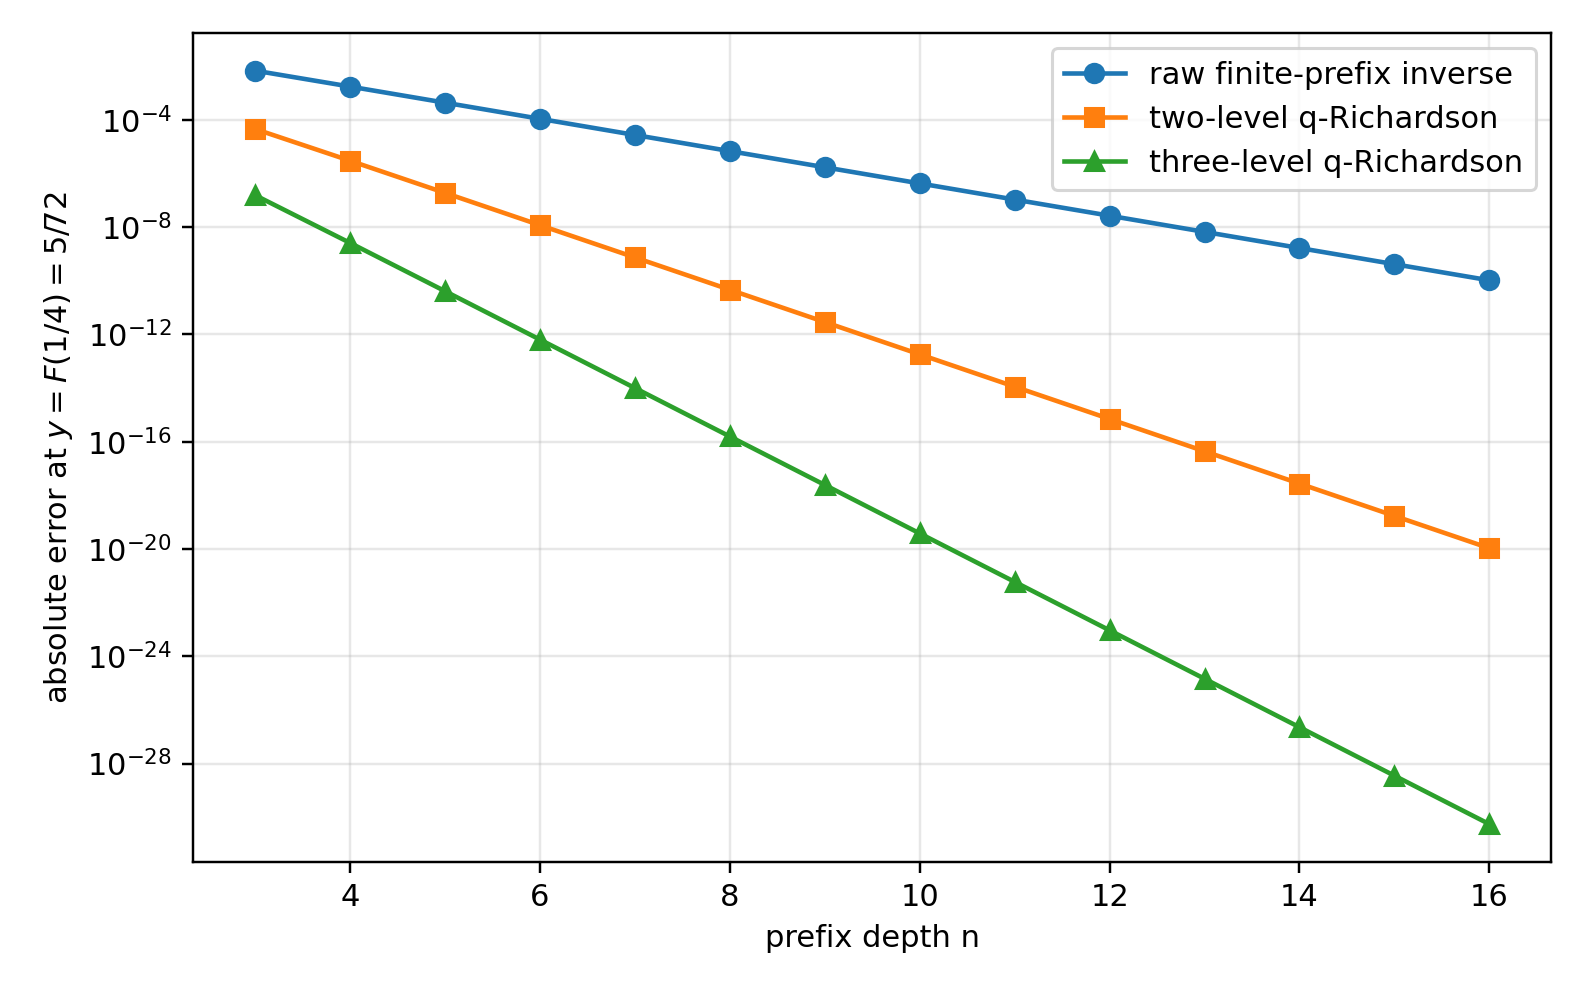
\includegraphics[width=0.92\textwidth]{assets/inverse-germs/figures/quarter_quantile_richardson.png}
\caption{Raw and accelerated errors at the exact output $F(1/4)=5/72$.  The
straight-line separation on the logarithmic scale reflects the exact geometric orders
$4^{-n}$, $16^{-n}$, and $64^{-n}$.}
\label{is:p1:fig:quarter-richardson}
\end{figure}

\subsection{Exact sign and two-sided bounds for every accelerated quarter error}

The preceding asymptotic constants can be strengthened to a finite-$n$ interpolation
statement.  Put
\begin{equation}
 f(Q):=\Delta_2(Q)=\frac{\sqrt{1+(64/9)Q}-1}{8}.
 \label{is:p1:eq:f-quarter-germ}
\end{equation}
For fixed $n$ and $s$, the quantity
$\mathcal G_{n,s}(5/72)-1/4$ is the value at $Q=0$ of the polynomial of degree
at most $s-1$ interpolating $f$ at the nodes
$4^{-n},4^{-(n+1)},\ldots,4^{-(n+s-1)}$.

\begin{theorem}[Positive accelerated errors and sharp finite-depth bounds]
\label{is:p1:thm:quarter-positive-bounds}
Let
\begin{equation}
 K_s:=\frac{C_{s-1}2^{-s^2+5s-2}}{9^s}.
 \label{is:p1:eq:Ks-quarter}
\end{equation}
For every $s\ge1$ and $n\ge3$,
\begin{equation}
 \boxed{
 0< K_s4^{-sn}\left(1+\frac{64}{9}4^{-n}\right)^{\frac12-s}
 <\mathcal G_{n,s}\!\left(\frac5{72}\right)-\frac14
 <K_s4^{-sn}.}
 \label{is:p1:eq:quarter-two-sided}
\end{equation}
In particular, the ratio of the exact error to its leading term is squeezed to one
inside an explicitly shrinking enclosure.
\end{theorem}

\begin{proof}
Let $p_{n,s-1}$ be the Lagrange interpolant just described.  The interpolation
remainder at zero gives a point $\xi_{n,s}\in(0,4^{-n})$ such that
\begin{equation}
 -p_{n,s-1}(0)
 =\frac{f^{(s)}(\xi_{n,s})}{s!}
   \prod_{j=0}^{s-1}(-4^{-(n+j)}).
 \label{is:p1:eq:Lagrange-remainder-quarter}
\end{equation}
Now
\begin{equation}
 f^{(s)}(Q)=\frac1{8}\left(\frac12\right)^{\!\underline{s}}
 \left(\frac{64}{9}\right)^s
 \left(1+\frac{64}{9}Q\right)^{\frac12-s},
 \label{is:p1:eq:f-quarter-derivative}
\end{equation}
where the falling factorial has sign $(-1)^{s-1}$.  The signs in
\eqref{is:p1:eq:Lagrange-remainder-quarter} therefore imply $p_{n,s-1}(0)>0$.
Using
\begin{equation}
 \frac{\left|\left(\frac12\right)^{\!\underline{s}}\right|}{8s!}
 \left(\frac{64}{9}\right)^s4^{-\binom s2}=K_s
 \label{is:p1:eq:Ks-identity}
\end{equation}
produces the middle expression in \eqref{is:p1:eq:quarter-two-sided} with
$\xi_{n,s}$ in place of either endpoint.  Since the exponent $1/2-s$ is
negative, evaluation at $0$ and $4^{-n}$ gives the two strict bounds.
\end{proof}

\begin{remark}
The positivity in \cref{is:p1:thm:quarter-positive-bounds} is not visible term-by-term in
\eqref{is:p1:eq:Catalan-qbinom-full}, whose tail alternates.  It is a consequence of the
complete monotonicity pattern of the derivatives of the square-root germ and the sign
of the Lagrange remainder.  This is one concrete place where exact interpolation gives
more information than formal Richardson cancellation.
\end{remark}

\begin{proposition}[Large-order Catalan coefficients]
\label{is:p1:prop:Catalan-large-order}
The Taylor coefficients of the quarter germ satisfy
\begin{equation}
 \boxed{
 \delta_{2,m}\sim
 (-1)^{m-1}\frac1{16\sqrt\pi}\left(\frac{64}{9}\right)^m m^{-3/2}.}
 \label{is:p1:eq:Catalan-large-order}
\end{equation}
Thus the branch point $Q=-9/64$ controls both the convergence radius and the
$m^{-3/2}$ algebraic prefactor.
\end{proposition}

\begin{proof}
Insert the classical Catalan asymptotic
$C_{m-1}\sim4^{m-1}/(\sqrt\pi\,m^{3/2})$ into
\eqref{is:p1:eq:Catalan-germ}.
\end{proof}

\subsection{A universal first coefficient at every inverse-dyadic anchor}

The leading displacement of the algebraic germ admits a particularly compact expression in
the dyadic moment numbers $d_r$ from \eqref{is:p1:eq:d-def}.

\begin{proposition}[First algebraic-germ coefficient]
\label{is:p1:prop:first-dyadic-germ-coefficient}
For every $r\ge2$,
\begin{equation}
 \boxed{
 \delta_{r,1}
 =\frac1{18}\frac{F''(2^{-r})}{F'(2^{-r})}
 =\frac{2^{r-1}(r-1)d_{r-2}}{9d_{r-1}}>0.}
 \label{is:p1:eq:first-dyadic-germ-coefficient}
\end{equation}
For $r=1$, $\Delta_1\equiv0$ and $\Gn(1/2)=1/2$ exactly.
\end{proposition}

\begin{proof}
The first equality is \eqref{is:p1:eq:c1} evaluated at $x_r$.  Formula
\eqref{is:p1:eq:dyadic-jet} gives
\[
 \frac{F''(x_r)}{F'(x_r)}
 =4\frac{F(2^{2-r})}{F(2^{1-r})}.
\]
Substitute \eqref{is:p1:eq:d-def} at indices $r-2$ and $r-1$ and simplify the powers
of two.  Positivity follows from $d_j>0$.  The case $r=1$ follows from symmetry
of every prefix density.
\end{proof}

The values $4/9$, $8/5$, and $40/9$ in
\eqref{is:p1:eq:Catalan-first}, \eqref{is:p1:eq:Delta3}, and \eqref{is:p1:eq:Delta4} are therefore
not isolated coincidences; they are the first members of a single exact rational
sequence controlled by adjacent dyadic moments.

% Source fragment: Inverse and sampling frontiers; prefix is.
\subsection{The two random series}

Recall the common variables from \cref{is:p1:eq:Y-prefix}: $(V_j)_{j\ge1}$
are independent and uniform on $[0,1]$, while $U_j=2V_j-1$ is uniform on
$[-1,1]$.  Thus
\begin{equation}
 X=\sum_{j\ge1}2^{-j}V_j,
 \qquad
 Y=\sum_{j\ge1}2^{-j}U_j=2X-1.
 \label{is:p2:eq:XY-series}
\end{equation}
Then $F$ is the distribution function of $X$ and $\RvachevUp$ is the density of $Y$.  Their moment
generating functions are entire:
\begin{align}
 L(t)&=\Expectation\EulerE^{tX}
 =\prod_{j\ge1}\frac{\EulerE^{t/2^j}-1}{t/2^j},
 \label{is:p2:eq:L-def}\\
 M(t)&=\Expectation\EulerE^{tY}
 =\prod_{j\ge1}\frac{\sinh(t/2^j)}{t/2^j}
 =\EulerE^{-t}L(2t).
 \label{is:p2:eq:M-def}
\end{align}
Self-similarity gives
\begin{equation}
 L(2t)=\frac{\EulerE^t-1}{t}L(t),
 \qquad
 M(2t)=\frac{\sinh t}{t}M(t).
 \label{is:p2:eq:mgf-refinement}
\end{equation}
On the imaginary axis,
\begin{equation}
 M(2\pi\ImaginaryUnit z)=\prod_{k\ge0}\SincPi(z/2^k)=:\PhiCyc(z),
 \qquad \SincPi u=\frac{\sin(\pi u)}{\pi u}.
 \label{is:p2:eq:M-Phi}
\end{equation}
Thus the moment problem and the infinite sinc product are two restrictions of the same entire
function.

\subsection{Moments and cumulants}

Write $\kappa_n(X)$ and $\kappa_n(Y)$ for cumulants.  The Bernoulli expansion of
$\log((\EulerE^t-1)/t)$ gives
\begin{align}
 \kappa_1(X)&=\frac12,
 &\kappa_{2r}(X)&=\frac{B_{2r}}{2r(4^r-1)},
 &\kappa_{2r+1}(X)&=0\quad(r\ge1),
 \label{is:p2:eq:X-cumulants}\\
 \kappa_1(Y)&=0,
 &\kappa_{2r}(Y)&=\frac{2^{2r-1}B_{2r}}{r(4^r-1)},
 &\kappa_{2r+1}(Y)&=0.
 \label{is:p2:eq:Y-cumulants}
\end{align}
The first centered moments are
\begin{equation}
 m_0=1,
 \quad m_2=\frac19,
 \quad m_4=\frac{19}{675},
 \quad m_6=\frac{583}{59535},
 \quad m_8=\frac{132809}{32531625}.
 \label{is:p2:eq:Y-moments}
\end{equation}
These established rational sequences will become coefficients in the exact finite-prefix expansion.

% Source fragment: Inverse and sampling frontiers; prefix is.
\section{Algebraic Taylor shadows of the inverse Fabius function}
\label{is:p2:sec:inverse-germs}

\subsection{The finite dyadic jet polynomial}

Fix a reduced dyadic point
\begin{equation}
 x_0=\frac{a}{2^N}\in(0,1),
 \qquad a\ \text{odd},
 \qquad y_0=F(x_0).
 \label{is:p2:eq:x0-y0}
\end{equation}
The derivative atlas \eqref{ii:eq:derivative-atlas} gives
\begin{equation}
 f_k:=F^{(k)}(x_0)
 =2^{\binom{k+1}{2}}\ThetaF(2^kx_0),
 \qquad
 Q_{x_0}(h):=\sum_{k=1}^{N}\frac{f_k}{k!}h^k.
 \label{is:p2:eq:Q-dyadic}
\end{equation}
For $k>N$, the argument $2^kx_0$ is an even integer, so the block formula
\eqref{ii:eq:theta-block} gives $F^{(k)}(x_0)=0$.  Hence $y_0+Q_{x_0}$
is the complete Taylor series of $F$ at $x_0$, not merely a finite-order
truncation.  The exact dyadic evaluator in \cref{is:p3:sec:qbinomial} shows
that every $f_k$ is rational.  Moreover $f_1=F'(x_0)>0$.

Define the smooth remainder
\begin{equation}
 \rho_{x_0}(h):=F(x_0+h)-y_0-Q_{x_0}(h).
 \label{is:p2:eq:rho-flat}
\end{equation}
Every derivative of $\rho_{x_0}$ at zero vanishes.  Nevertheless
$\rho_{x_0}$ is not identically zero on any neighborhood: otherwise $F$
would agree locally with a polynomial, contrary to \cref{ne:thm:nowhere}.

\begin{theorem}[Dyadic algebraic inverse germ; \statusnew]
\label{is:p2:thm:algebraic-inverse-germ}
There is a unique real-analytic germ $S_{x_0}$ at zero satisfying
\begin{equation}
 Q_{x_0}(S_{x_0}(z))=z,
 \qquad S_{x_0}(0)=0.
 \label{is:p2:eq:S-inverse}
\end{equation}
It is algebraic over $\RationalNumbers(z)$.  On a neighborhood of zero,
\begin{equation}
 \boxed{
 \FabiusQuantile(y_0+z)
 =x_0+S_{x_0}(z)+R_{x_0}(z),}
 \label{is:p2:eq:G-shadow}
\end{equation}
where $R_{x_0}$ is smooth, flat at zero, and nonzero on every neighborhood
of zero.  Consequently the complete Taylor series of $\FabiusQuantile$ at
$y_0$ has positive radius and an algebraic sum, but that sum does not
represent $\FabiusQuantile$ on any neighborhood.
\end{theorem}

\begin{proof}
Because $Q_{x_0}'(0)=f_1>0$, the real-analytic inverse-function theorem
gives a unique analytic inverse germ $S_{x_0}$.  It satisfies the polynomial
equation $Q_{x_0}(w)-z=0$ over $\RationalNumbers(z)$, so it is algebraic.

Put
\[
 H(z):=\FabiusQuantile(y_0+z)-x_0.
\]
Then $H(0)=0$, $H'(0)=1/f_1>0$, and
\begin{equation}
 z=Q_{x_0}(H(z))+\rho_{x_0}(H(z)).
 \label{is:p2:eq:H-flat-reversion}
\end{equation}
Fa\`a di Bruno's formula shows directly that $\rho_{x_0}\comp H$ is flat:
every term in every derivative at zero contains a derivative of
$\rho_{x_0}$ at $H(0)=0$.  Taking formal Taylor series in
\eqref{is:p2:eq:H-flat-reversion} therefore gives
$Q_{x_0}(\mathsf T_H(z))=z$.  A formal series with zero constant term and
nonzero linear coefficient has a unique compositional inverse; hence
$\mathsf T_H=\mathsf T_{S_{x_0}}$.  Thus
$R_{x_0}:=H-S_{x_0}$ is smooth and flat.

If $R_{x_0}$ vanished throughout some neighborhood, then
$\FabiusQuantile$ would agree there with the analytic germ
$x_0+S_{x_0}$.  Its derivative at $y_0$ is positive, so the analytic
inverse-function theorem would make $F$ analytic at $x_0$, again
contradicting \cref{ne:thm:nowhere}.  Therefore the flat remainder is
nonzero in every neighborhood.  Finally, its vanishing Taylor series shows
that the Taylor series of $\FabiusQuantile$ is precisely the convergent
algebraic series of $S_{x_0}$.
\end{proof}

\begin{resultbox}[Analytic shadow versus the actual inverse]
At each dyadic output $F(a/2^N)$, every derivative of the inverse is encoded
by a finite rational polynomial, yet the actual inverse differs from that
algebraic germ by a nontrivial flat function.  Positive Taylor radius and
local analyticity are therefore sharply different properties here.
\end{resultbox}

\subsection{Lagrange--B\"urmann and Bell formulas}

Factor
\begin{equation}
 Q_{x_0}(u)=u\varphi_{x_0}(u),
 \qquad
 \varphi_{x_0}(0)=f_1>0.
 \label{is:p2:eq:Q-phi}
\end{equation}
The coefficients of the algebraic inverse are completely explicit.

\begin{theorem}[All inverse derivatives at dyadic outputs; \statusnew]
\label{is:p2:thm:inverse-derivatives}
For every $m\ge1$,
\begin{equation}
 \boxed{
 \FabiusQuantile^{(m)}(y_0)
 =(m-1)!\,[u^{m-1}]\,\varphi_{x_0}(u)^{-m}.
 }
 \label{is:p2:eq:Lagrange-inverse-derivative}
\end{equation}
Equivalently, if $g_m=\FabiusQuantile^{(m)}(y_0)$ and $B_{m,k}$ denotes the partial exponential Bell
polynomial, then
\begin{align}
 g_1&=\frac1{f_1},
 \label{is:p2:eq:g1}\\
 g_m&=-\frac1{f_1}
 \sum_{k=2}^{\min(m,N)}f_k
 B_{m,k}(g_1,g_2,\ldots,g_{m-k+1})
 \qquad(m\ge2).
 \label{is:p2:eq:Bell-inverse-recurrence}
\end{align}
In particular, every $\FabiusQuantile^{(m)}(y_0)$ is rational.
\end{theorem}

\begin{proof}
The Lagrange--B\"urmann formula for the inverse of $z=u\varphi_{x_0}(u)$ gives
\[
 [z^m]S_{x_0}(z)=\frac1m[u^{m-1}]\varphi_{x_0}(u)^{-m}.
\]
Multiplication by $m!$ proves \eqref{is:p2:eq:Lagrange-inverse-derivative}.  For the Bell recurrence,
differentiate $F(\FabiusQuantile(y))=y$ $m$ times at $y=y_0$.  Fa\`a di Bruno gives
\[
 \sum_{k=1}^{m} f_k B_{m,k}(g_1,\ldots,g_{m-k+1})=0\qquad(m\ge2).
\]
Since $B_{m,1}=g_m$, solving for the newest derivative gives
\eqref{is:p2:eq:Bell-inverse-recurrence}.  All inputs are rational.
\end{proof}

\begin{remark}
The formulas use two different Bell-polynomial roles in the same theory.  Partial Bell polynomials
invert composition in \eqref{is:p2:eq:Bell-inverse-recurrence}; complete Bell polynomials will invert a
moment generating function in \cref{is:p2:sec:appell}.  The two appearances are not cosmetic variants:
one organizes set partitions by the number of blocks, while the other sums over all block counts.
\end{remark}

\subsection{The midpoint and quarter-point shadows}

At $x_0=y_0=1/2$, reflection gives $F'(1/2)=2$ and makes every higher
derivative vanish.  Thus
\begin{equation}
 Q_{1/2}(h)=2h,
 \qquad
 S_{1/2}(z)=\frac z2,
 \qquad
 \FabiusQuantile(1/2+z)=\frac12+\frac z2+R_{1/2}(z).
 \label{is:p2:eq:midpoint-shadow}
\end{equation}
The reflection law for $\FabiusQuantile$ makes $R_{1/2}$ odd;
\cref{is:p2:thm:algebraic-inverse-germ} makes it flat and nonzero in every
neighborhood.  Hence every derivative beyond the first vanishes even though
the inverse is not affine on any interval.

The first nonlinear shadow has a classical coefficient sequence.

\begin{theorem}[Catalan inverse jet at $F(1/4)$; \statusnew]
\label{is:p2:thm:Catalan-quarter}
One has
\begin{equation}
 F(1/4)=\frac5{72},
 \qquad F'(1/4)=1,
 \qquad F''(1/4)=8,
 \qquad F^{(m)}(1/4)=0\quad(m\ge3).
 \label{is:p2:eq:quarter-jet}
\end{equation}
Consequently
\begin{equation}
 Q_{1/4}(h)=h+4h^2,
 \qquad
 S_{1/4}(z)=\frac{\sqrt{1+16z}-1}{8},
 \label{is:p2:eq:quarter-shadow}
\end{equation}
and, for every $m\ge1$,
\begin{equation}
 \boxed{
 \FabiusQuantile^{(m)}(5/72)
 =m!(-1)^{m-1}4^{m-1}C_{m-1},
 \qquad C_r=\frac1{r+1}\binom{2r}{r}.}
 \label{is:p2:eq:Catalan-derivatives}
\end{equation}
In particular,
\begin{equation}
 \AbsoluteValue{\FabiusQuantile^{(m)}(5/72)}
 \sim\frac{m!\,16^{m-1}}{\sqrt\pi\,(m-1)^{3/2}}.
 \label{is:p2:eq:Catalan-asymptotic}
\end{equation}
\end{theorem}

\begin{proof}
The exact dyadic formula of \cref{is:p3:sec:qbinomial} gives
$F(1/4)=5/72$.  The derivative atlas and the values
$\ThetaF(1/2)=F(1/2)=1/2$ and $\ThetaF(1)=\RvachevUp(0)=1$ give the first
two derivatives in \eqref{is:p2:eq:quarter-jet}.  For $m\ge3$, the argument
$2^m/4$ is an even integer, so \eqref{ii:eq:theta-block} gives zero.
Solving $z=h+4h^2$ for the branch with $h(0)=0$ proves
\eqref{is:p2:eq:quarter-shadow}.  The Catalan generating function, after
the substitution $w=-4z$, is
\[
 \frac{\sqrt{1+16z}-1}{8}
 =\sum_{m\ge1}(-1)^{m-1}4^{m-1}C_{m-1}z^m.
\]
Because the flat remainder has zero derivatives, multiplying the coefficient
of $z^m$ by $m!$ proves \eqref{is:p2:eq:Catalan-derivatives}.  Finally use
$C_r\sim4^r/(\sqrt\pi\,r^{3/2})$.
\end{proof}

For reference, the first values are
\[
 \FabiusQuantile'(5/72)=1,
 \quad \FabiusQuantile''(5/72)=-8,
 \quad \FabiusQuantile^{(3)}(5/72)=192,
 \quad \FabiusQuantile^{(4)}(5/72)=-7680.
\]
These rapidly growing derivatives belong to the algebraic square-root
shadow; they do not assert local analyticity of the actual inverse.

\subsection{The eighth-point cubic and the singularity atlas}

At $x_0=1/8$, exact dyadic evaluation and the derivative atlas give
\begin{equation}
 F(1/8)=\frac1{288},
 \qquad F'(1/8)=\frac5{36},
 \qquad F''(1/8)=4,
 \qquad F^{(3)}(1/8)=64.
 \label{is:p2:eq:eighth-jet}
\end{equation}
Thus the inverse Taylor series at $1/288$ is the origin branch of
\begin{equation}
 z=\frac5{36}h+2h^2+\frac{32}{3}h^3,
 \label{is:p2:eq:eighth-cubic}
\end{equation}
and \cref{is:p2:thm:inverse-derivatives} specializes to
\begin{equation}
 \FabiusQuantile^{(m)}(1/288)
 =(m-1)![u^{m-1}]
 \left(\frac5{36}+2u+\frac{32}{3}u^2\right)^{-m}.
 \label{is:p2:eq:eighth-coeff}
\end{equation}

The finite polynomial $Q_{x_0}$ also turns large-order derivative analysis
into finite algebraic geometry.  Singularities of its inverse branch occur
at critical values $Q_{x_0}(u_c)$ with $Q_{x_0}'(u_c)=0$ (or at infinity).
A nearest simple critical value produces the universal square-root
$m^{-3/2}$ coefficient factor seen above; higher critical multiplicity
produces the corresponding Puiseux exponent.

\begin{problem}[Dyadic inverse singularity atlas]
\label{is:p2:prob:dyadic-singularity-atlas}
For every reduced dyadic $a/2^N$, classify the critical values of
$Q_{a/2^N}$, determine those visible from the origin branch and hence its
exact convergence radius, and describe the Galois and $2$-adic structure of
the associated Puiseux constants.  The cases $N=2$ and $N=3$ are the
quadratic Catalan and cubic examples above.
\end{problem}

% Source fragment: Inverse and sampling frontiers; prefix is.
\section{Kabaya--Iri polynomials and the Rvachev Appell inverse}
\label{is:p2:sec:appell}

\subsection{The external precursor and the normalization used here}

Lee's scaling-polynomial construction associates to a compactly supported probability density
$\phi$ the Appell sequence generated by
$\EulerE^{xt}/\FourierAngular{\phi}(\ImaginaryUnit t)$ and proves its biorthogonality
to the distributional derivatives of $\phi$.  For the up-function, these are the Kabaya--Iri
polynomials.  In the Fabius normalization used in this report, it is convenient to distinguish the
uncentered law $X\in[0,1]$ from the centered law $Y=2X-1\in[-1,1]$.

\begin{definition}[Kabaya--Iri and centered Rvachev--Appell polynomials]
\label{is:p2:def:Appell-polys}
Define $P_n,A_n\in\RationalNumbers[x]$ by
\begin{align}
 \frac{\EulerE^{xt}}{L(t)}
 &=\sum_{n\ge0}P_n(x)\frac{t^n}{n!},
 \label{is:p2:eq:P-generating}\\
 \frac{\EulerE^{xt}}{M(t)}
 &=\sum_{n\ge0}A_n(x)\frac{t^n}{n!}.
 \label{is:p2:eq:A-generating}
\end{align}
\end{definition}

The affine change $M(t)=\EulerE^{-t}L(2t)$ gives
\begin{equation}
 \boxed{
 A_n(x)=2^nP_n\!\left(\frac{x+1}{2}\right),
 \qquad
 P_n(x)=2^{-n}A_n(2x-1).
 }
 \label{is:p2:eq:A-P-affine}
\end{equation}
Thus the sequence $P_n$ is the known Kabaya--Iri sequence, while $A_n$ is its symmetric Rvachev
normalization.  The centering eliminates every odd cumulant and makes the pole analysis in
\cref{is:p2:sec:poles} transparent.

\subsection{Appell, mean-value, and biorthogonality identities}

\begin{proposition}[Classical Appell package; \statuslit]
\label{is:p2:prop:Appell-package}
For $n\ge1$ and, in the biorthogonality identities, every integer $r\ge0$,
\begin{align}
 P_n'(x)&=nP_{n-1}(x),
 &A_n'(x)&=nA_{n-1}(x),
 \label{is:p2:eq:Appell-derivative}\\
 P_n(x+y)&=\sum_{k=0}^n\binom nkP_k(x)y^{n-k},
 &A_n(x+y)&=\sum_{k=0}^n\binom nkA_k(x)y^{n-k}.
 \label{is:p2:eq:Appell-translation}
\end{align}
The polynomial averaging operators are inverted exactly:
\begin{equation}
 \boxed{
 \Expectation\,P_n(x+X)=x^n,
 \qquad
 \Expectation\,A_n(x+Y)=x^n.
 }
 \label{is:p2:eq:mean-value-inversion}
\end{equation}
If $f_X=F'$ is the density of $X$, then in the distributional sense
\begin{equation}
 \left\langle(-1)^r f_X^{(r)},\frac{P_n}{n!}\right\rangle=\delta_{rn}.
 \label{is:p2:eq:P-biorthogonal}
\end{equation}
Equivalently, for the centered density $\RvachevUp$,
\begin{equation}
 \int_{-1}^{1}(-1)^r\RvachevUp^{(r)}(x)\frac{A_n(x)}{n!}\,\Differential x
 =\delta_{rn}.
 \label{is:p2:eq:A-biorthogonal}
\end{equation}
\end{proposition}

\begin{proof}
Differentiate the generating functions with respect to $x$ to obtain
\eqref{is:p2:eq:Appell-derivative}; multiply by $\EulerE^{yt}$ to obtain
\eqref{is:p2:eq:Appell-translation}.  For the mean-value identities,
\[
 \Expectation\sum_{n\ge0}P_n(x+X)\frac{t^n}{n!}
 =\Expectation\frac{\EulerE^{(x+X)t}}{L(t)}=\EulerE^{xt},
\]
and similarly for $A_n$.  Here is the distributional calculation, including
the case in which the order of differentiation exceeds the polynomial degree.
Regard $f_X$ as a compactly supported smooth function on $\RealNumbers$.  By
the definition of a distributional derivative and repeated integration by
parts,
\begin{equation}
 \left\langle(-1)^r f_X^{(r)},\frac{P_n}{n!}\right\rangle
 =\left\langle f_X,
   \left(\frac{P_n}{n!}\right)^{(r)}\right\rangle.
 \label{is:p2:eq:P-biorthogonal-calculation}
\end{equation}
There are no boundary terms in this formulation.  Iterating the Appell rule
shows that the polynomial on the right is
\[
 \left(\frac{P_n}{n!}\right)^{(r)}
 =\begin{cases}
   P_{n-r}/(n-r)!,&0\le r\le n,\\
   0,&r>n.
  \end{cases}
\]
For $r\le n$, the right side of
\eqref{is:p2:eq:P-biorthogonal-calculation} is therefore
\[
 \frac{\Expectation P_{n-r}(X)}{(n-r)!}
 =\delta_{rn},
\]
where the second equality is \eqref{is:p2:eq:mean-value-inversion} at $x=0$
(the expectation is $1$ for $n-r=0$ and $0$ for $n-r>0$); for $r>n$ the
pairing is zero because the test polynomial has vanished.  This proves
\eqref{is:p2:eq:P-biorthogonal} for every $r\ge0$.

For completeness, the centered identity is exactly the affine transport of
this calculation.  Since $Y=2X-1$,
\[
 \RvachevUp(y)=\frac12 f_X\!\left(\frac{y+1}{2}\right),
 \qquad
 \RvachevUp^{(r)}(y)=2^{-r-1}f_X^{(r)}\!\left(\frac{y+1}{2}\right),
\]
while \eqref{is:p2:eq:A-P-affine} gives
$A_n(y)=2^nP_n((y+1)/2)$.  Thus the substitution $y=2u-1$ gives
\begin{align*}
 \int_{-1}^{1}(-1)^r\RvachevUp^{(r)}(y)
       \frac{A_n(y)}{n!}\,\Differential y
 &=2^{n-r}
   \left\langle(-1)^r f_X^{(r)},\frac{P_n}{n!}\right\rangle\\
 &=2^{n-r}\delta_{rn}=\delta_{rn},
\end{align*}
which is \eqref{is:p2:eq:A-biorthogonal}.
\end{proof}

\begin{remark}
Equation \eqref{is:p2:eq:mean-value-inversion} is an exact polynomial deconvolution formula.  The operator
$\mathcal T_Y:p\mapsto\Expectation p(\,\cdot+Y)$ is triangular on $\RationalNumbers[x]$ with ones on its diagonal;
$A_n=\mathcal T_Y^{-1}x^n$.  This is the linear inverse problem paired with
quantile inversion in the common platform of \cref{sec:common-platform}.
\end{remark}

\subsection{Bell reconstruction from Bernoulli cumulants}

Set
\begin{equation}
 \alpha_n=A_n(0),
 \qquad
 \frac1{M(t)}=\sum_{n\ge0}\alpha_n\frac{t^n}{n!}.
 \label{is:p2:eq:alpha-def}
\end{equation}
Symmetry gives $\alpha_{2r+1}=0$.  If $\ExponentialCompleteBellPolynomial{n}$ denotes the complete exponential Bell polynomial,
then \eqref{is:p2:eq:Y-cumulants} yields
\begin{equation}
 \boxed{
 \alpha_n=\ExponentialCompleteBellPolynomial{n}\bigl(-\kappa_1(Y),-\kappa_2(Y),\ldots,-\kappa_n(Y)\bigr).
 }
 \label{is:p2:eq:alpha-Bell}
\end{equation}
Equivalently,
\begin{equation}
 \alpha_0=1,
 \qquad
 \alpha_n=-\sum_{j=1}^n\binom{n-1}{j-1}\kappa_j(Y)\alpha_{n-j}.
 \label{is:p2:eq:alpha-recurrence}
\end{equation}
The first constants are
\begin{equation}
 \alpha_0=1,
 \quad \alpha_2=-\frac19,
 \quad \alpha_4=\frac{31}{675},
 \quad \alpha_6=-\frac{2347}{59535},
 \quad \alpha_8=\frac{1904369}{32531625}.
 \label{is:p2:eq:alpha-first}
\end{equation}
The Appell translation law then gives
\begin{equation}
 A_n(x)=\sum_{k=0}^n\binom nk\alpha_{n-k}x^k.
 \label{is:p2:eq:A-from-alpha}
\end{equation}
For reference,
\begin{equation}
\begin{aligned}
 A_0(x)&=1,\\
 A_1(x)&=x,\\
 A_2(x)&=x^2-\frac19,\\
 A_3(x)&=x^3-\frac13x,\\
 A_4(x)&=x^4-\frac23x^2+\frac{31}{675},\\
 A_5(x)&=x^5-\frac{10}{9}x^3+\frac{31}{135}x,\\
 A_6(x)&=x^6-\frac53x^4+\frac{31}{45}x^2-\frac{2347}{59535}.
\end{aligned}
\label{is:p2:eq:A-first-polys}
\end{equation}
Using \eqref{is:p2:eq:A-P-affine}, the first uncentered polynomials are
\begin{equation}
\begin{aligned}
 P_0(x)&=1,\\
 P_1(x)&=x-\frac12,\\
 P_2(x)&=x^2-x+\frac29,\\
 P_3(x)&=x^3-\frac32x^2+\frac23x-\frac1{12},\\
 P_4(x)&=x^4-2x^3+\frac43x^2-\frac13x+\frac{16}{675},\\
 P_5(x)&=x^5-\frac52x^4+\frac{20}{9}x^3-\frac56x^2+\frac{16}{135}x-\frac1{270}.
\end{aligned}
\label{is:p2:eq:P-first-polys}
\end{equation}
These agree with Lee's displayed Kabaya--Iri list through degree five.

\subsection{Bernoulli refinement recurrences}

The self-similarity identities \eqref{is:p2:eq:mgf-refinement} become polynomial recurrences when the
reciprocal generating functions are compared.

\begin{proposition}[Bernoulli refinement of the Appell sequences]
\label{is:p2:prop:Bernoulli-refinement}
Let $B_k$ be defined by $t/(\EulerE^t-1)=\sum B_kt^k/k!$, and let
$c_{2r}=2(1-2^{2r-1})B_{2r}$ be the exponential coefficients of
$t/\sinh t$.  Then
\begin{align}
 2^nP_n(x)
 &=\sum_{k=0}^n\binom nkB_kP_{n-k}(2x),
 \label{is:p2:eq:P-Bernoulli-refinement}\\
 2^nA_n(x)
 &=\sum_{r=0}^{\Floor{n/2}}
   \binom n{2r}c_{2r}A_{n-2r}(2x).
 \label{is:p2:eq:A-Bernoulli-refinement}
\end{align}
\end{proposition}

\begin{proof}
Substitute \eqref{is:p2:eq:mgf-refinement} into the defining generating functions:
\begin{align*}
 \frac{\EulerE^{2xt}}{L(2t)}
 &=\frac{t}{\EulerE^t-1}\frac{\EulerE^{2xt}}{L(t)},\\
 \frac{\EulerE^{2xt}}{M(2t)}
 &=\frac{t}{\sinh t}\frac{\EulerE^{2xt}}{M(t)}.
\end{align*}
Coefficient comparison gives the two formulas.
\end{proof}

\begin{remark}
The repository's Bernoulli recurrences usually govern moments, reciprocal sine products, or saddle
coefficients.  Here the same Bernoulli numbers govern a polynomial eigenbasis for the adjoint
Rvachev averaging operator.  The recurrence is a direct algebraic shadow of dyadic refinement.
\end{remark}

\subsection{A dyadic logistic dual}

The complete Bell signs in \eqref{is:p2:eq:alpha-first} admit a probabilistic explanation that appears not
to have been recorded for the Rvachev law.

Let $\Lambda$ be a standard logistic random variable with density
\begin{equation}
 \ell(x)=\frac{\EulerE^{-x}}{(1+\EulerE^{-x})^2}.
 \label{is:p2:eq:logistic-density}
\end{equation}
The beta integral gives
\begin{equation}
 \Expectation\EulerE^{\ImaginaryUnit t\Lambda}
 =\Gamma(1+\ImaginaryUnit t)\Gamma(1-\ImaginaryUnit t)
 =\frac{\pi t}{\sinh(\pi t)}.
 \label{is:p2:eq:logistic-cf}
\end{equation}
Let $(\Lambda_j)_{j\ge1}$ be independent copies and define
\begin{equation}
 Z=\sum_{j\ge1}\frac{\Lambda_j}{\pi2^j}.
 \label{is:p2:eq:Z-logistic}
\end{equation}
The series converges in $L^2$ and almost surely.

\begin{theorem}[Logistic dual of the Rvachev law; \statusnew]
\label{is:p2:thm:logistic-dual}
For real $t$,
\begin{equation}
 \boxed{
 \Expectation\EulerE^{\ImaginaryUnit tZ}
 =\prod_{j\ge1}\frac{t/2^j}{\sinh(t/2^j)}
 =\frac1{M(t)}.
 }
 \label{is:p2:eq:Z-cf}
\end{equation}
Consequently, as polynomial identities,
\begin{align}
 A_n(x)&=\Expectation\,(x+\ImaginaryUnit Z)^n,
 \label{is:p2:eq:A-logistic-moment}\\
 P_n(x)&=\Expectation\left(x-\frac12+\frac{\ImaginaryUnit Z}{2}\right)^n.
 \label{is:p2:eq:P-logistic-moment}
\end{align}
In particular,
\begin{equation}
 \boxed{
 \alpha_{2m}=(-1)^m\Expectation Z^{2m},
 \qquad (-1)^m\alpha_{2m}>0.
 }
 \label{is:p2:eq:alpha-sign}
\end{equation}
\end{theorem}

\begin{proof}
We first record the integrability needed to turn the formal coefficient
comparison into an analytic one.  The logistic density satisfies
$\ell(x)\le\EulerE^{-\AbsoluteValue{x}}$, so
$\Expectation\EulerE^{s\AbsoluteValue{\Lambda}}<\infty$ for $0\le s<1$.
Fix $0<a<2\pi$ and put $s_j=a/(\pi2^j)$.  Since
\[
 \log\Expectation\EulerE^{s\AbsoluteValue{\Lambda}}=\BigO(s)
 \qquad(s\downarrow0),
\]
independence and monotone convergence give
\begin{equation}
 \Expectation\exp\!\left(
   a\sum_{j\ge1}\frac{\AbsoluteValue{\Lambda_j}}{\pi2^j}
  \right)
 =\prod_{j\ge1}\Expectation\EulerE^{s_j\AbsoluteValue{\Lambda}}
 <\infty.
 \label{is:p2:eq:Z-exponential-moment}
\end{equation}
In particular, the defining series for $Z$ converges absolutely almost surely
and $\Expectation\EulerE^{a\AbsoluteValue Z}<\infty$ for every
$0<a<2\pi$.

Let $Z_N=\sum_{j=1}^N\Lambda_j/(\pi2^j)$.  Independence and
\eqref{is:p2:eq:logistic-cf} give, for real $t$,
\[
 \Expectation\EulerE^{\ImaginaryUnit tZ_N}
 =\prod_{j=1}^{N}\frac{t/2^j}{\sinh(t/2^j)}.
\]
The almost-sure convergence $Z_N\to Z$ and bounded convergence pass the left
side to $\Expectation\EulerE^{\ImaginaryUnit tZ}$.  On the right,
\[
 \log\!\left(\frac{w}{\sinh w}\right)=\BigO(w^2)
 \qquad(w\to0),
\]
so the product converges locally uniformly for complex $t$ in
$\AbsoluteValue t<2\pi$; its factors are nonzero there, and its product is
the reciprocal of the locally uniformly convergent product defining $M(t)$.
The exponential-moment bound makes
$t\mapsto\Expectation\EulerE^{\ImaginaryUnit tZ}$ holomorphic on every strip
$\AbsoluteValue{\operatorname{Im}t}<a<2\pi$.  Thus the identity theorem
extends the equality from real $t$ throughout the disk
$\AbsoluteValue t<2\pi$, and in particular proves \eqref{is:p2:eq:Z-cf}.

It remains to justify coefficient comparison.  The exponential-moment bound
\eqref{is:p2:eq:Z-exponential-moment} makes
\[
 t\longmapsto \Expectation\EulerE^{t(x+\ImaginaryUnit Z)}
\]
analytic near zero.  Indeed, on any smaller closed disk and for every $n$,
the $n$th derivative of the integrand is dominated by
\[
 (\AbsoluteValue x+\AbsoluteValue Z)^n
 \EulerE^{r(\AbsoluteValue x+\AbsoluteValue Z)},
\]
which is integrable after choosing $r<a<2\pi$.  Differentiation under the
expectation is therefore valid to every order.  Consequently
\[
 \frac{\EulerE^{xt}}{M(t)}
 =\EulerE^{xt}\Expectation\EulerE^{\ImaginaryUnit tZ}
 =\Expectation\EulerE^{t(x+\ImaginaryUnit Z)}
 =\sum_{n\ge0}\Expectation(x+\ImaginaryUnit Z)^n\frac{t^n}{n!}
\]
near zero, and comparison with \eqref{is:p2:eq:A-generating} proves
\eqref{is:p2:eq:A-logistic-moment} for every real $x$, hence as a polynomial
identity.  Substituting $2x-1$ and using
\eqref{is:p2:eq:A-P-affine} gives \eqref{is:p2:eq:P-logistic-moment}.
Finally $Z$ is symmetric and nondegenerate; indeed, independence and
$\Variance(\Lambda)=\pi^2/3$ give
$\Variance(Z)=\sum_{j\ge1}(3\cdot4^j)^{-1}=1/9$.
Therefore setting $x=0$ gives
$\alpha_{2m}=(-1)^m\Expectation Z^{2m}$ and
$\Expectation Z^{2m}>0$ (with the value $1$ when $m=0$), proving
\eqref{is:p2:eq:alpha-sign}.
\end{proof}

\begin{resultbox}[A duality of compact and noncompact laws]
The Rvachev variable $Y$ is compactly supported and has moment generating function $M$.  Its
polynomial deconvolution sequence is represented by imaginary moments of the noncompact variable
$Z$, an infinite dyadic sum of logistic variables, whose characteristic function is $M^{-1}$.
Thus $M(t)^{-1}=\PhiAng(-\ImaginaryUnit t)^{-1}$ is not merely a formal
series: on the real $t$-axis it is the positive-definite characteristic
function of $Z$.  This is the reciprocal \emph{hyperbolic}-sinc product, or
equivalently the analytic continuation of the reciprocal trigonometric-sinc
product to the imaginary Fourier axis.  The function $1/\PhiAng(\xi)$ on the
real Fourier axis has poles and is not a characteristic function.
\end{resultbox}

\subsection{Operator interpretation}

Let $D=\Differential/\Differential x$.  On polynomials,
\begin{equation}
 \mathcal T_Y=\Expectation\EulerE^{YD}=M(D),
 \qquad
 \mathcal T_Y^{-1}=M(D)^{-1}=\Expectation\EulerE^{\ImaginaryUnit ZD}.
 \label{is:p2:eq:operator-deconvolution}
\end{equation}
Therefore
\begin{equation}
 A_n=M(D)^{-1}x^n.
 \label{is:p2:eq:A-operator}
\end{equation}
This identity packages the mean-value theorem, the logistic dual, and the Appell derivative rule in
one line.  It also prepares the finite Barnes and Thue--Morse difference calculus: replacing $M$ by
a finite product replaces the infinite-order differential operator by a finite product of Bernoulli
operators.

\section{Exact distribution laws for all Rvachev derivatives}
\label{rvd:sec:derivative-distribution}

The latest formal development yields a distributional theorem stronger than
any individual derivative norm or moment identity.  It is logically distinct
from Appell biorthogonality: the test function below is applied to the
\emph{value} of a derivative, not multiplied by an Appell polynomial in the
spatial variable.

For $n\ge0$, $0\le k<2^n$, and $-1\le y\le1$, put
\[
 c_{n,k}(y):=-1+\frac{2k+1+y}{2^n},
 \qquad \mathcal D_n:=2^{\binom{n+1}{2}},
\]
and let $\BinaryDigitSum(k)$ be the binary digit sum.

\begin{theorem}[Cell tiling and derivative pushforward laws]
\label{rvd:thm:derivative-distribution}
The $n$th derivative of the Rvachev function $u$ satisfies
\begin{equation}
 u^{(n)}(c_{n,k}(y))=\mathcal D_n(-1)^{\BinaryDigitSum(k)}u(y).
 \label{rvd:eq:cell-tiling}
\end{equation}
Consequently, for every continuous real- or Banach-valued test function $H$,
\begin{equation}
 \int_{-1}^{1}H\!\left(\mathcal D_n^{-1}|u^{(n)}(x)|\right)\Differential x
 =\int_{-1}^{1}H(u(y))\Differential y.
 \label{rvd:eq:absolute-law}
\end{equation}
For $n\ge1$ the signed normalized law is the symmetric half-mixture
\begin{equation}
 \int_{-1}^{1}H\!\left(\mathcal D_n^{-1}u^{(n)}(x)\right)\Differential x
 =\frac12\int_{-1}^{1}\bigl(H(u(y))+H(-u(y))\bigr)\Differential y.
 \label{rvd:eq:signed-law}
\end{equation}
Equivalently, these are equalities of Borel pushforward measures under
Lebesgue measure restricted to $[-1,1]$.  In particular, for $m\in\NaturalNumbers$,
\begin{equation}
 \int_{-1}^{1}(u^{(n)}(x))^m\Differential x
 =2^{-n}(1+(-1)^m)^n\mathcal D_n^m
  \int_{-1}^{1}u(y)^m\Differential y,
 \label{rvd:eq:signed-moments}
\end{equation}
and, for every real $p\ge0$,
\begin{equation}
 \int_{-1}^{1}|u^{(n)}(x)|^p\Differential x
 =\mathcal D_n^p\int_{-1}^{1}u(y)^p\Differential y.
 \label{rvd:eq:absolute-moments}
\end{equation}
\end{theorem}

\begin{proof}
The derivative atlas gives exactly \eqref{rvd:eq:cell-tiling}; the affine map
$c_{n,k}$ carries $[-1,1]$ onto the $k$th of the $2^n$ adjacent level-$n$
cells and has Jacobian $2^{-n}$.  Partitioning $[-1,1]$ into these cells and
substituting $x=c_{n,k}(y)$ therefore gives
\[
 \int_{-1}^{1}H(u^{(n)}(x))\Differential x
 =2^{-n}\sum_{k=0}^{2^n-1}
   \int_{-1}^{1}H\!\left(\mathcal D_n(-1)^{\BinaryDigitSum(k)}u(y)\right)\Differential y.
\]
Taking absolute values erases every sign, and the $2^n$ equal summands cancel
the Jacobian, proving \eqref{rvd:eq:absolute-law}.  For $n\ge1$, toggling the
lowest binary digit pairs the indices with opposite Thue--Morse signs; hence
exactly $2^{n-1}$ signs are positive and $2^{n-1}$ are negative.  This proves
\eqref{rvd:eq:signed-law}.  Continuous test functions determine finite Borel
measures on the compact range, so the integral identities imply the stated
pushforward equalities.  Finally take $H(t)=t^m$ and use the Boolean-cube
identity
\[
 \sum_{k=0}^{2^n-1}\bigl((-1)^m\bigr)^{\BinaryDigitSum(k)}
 =(1+(-1)^m)^n
\]
to obtain \eqref{rvd:eq:signed-moments}; take $H(t)=t^p$ in the nonnegative
absolute law to obtain \eqref{rvd:eq:absolute-moments}.
\end{proof}

The cell identity, Banach-valued test-function formulas, both pushforward
equalities, and all nonnegative real absolute moments are machine checked in
\path{FabiusFunction.RvachevDerivativeDistribution}; the principal
declarations are \path{iteratedDeriv_rvachev_cell},
\path{map_normalized_iteratedDeriv_rvachev_restrict_Icc}, and
\path{map_normalized_abs_iteratedDeriv_rvachev_restrict_Icc}.

\section{Finite dyadic prefixes as Barnes--Bernoulli polynomials}
\label{is:p2:sec:barnes}

\subsection{Finite random sums and finite Appell inverses}

For $N\ge0$, define the convolution prefixes
\begin{equation}
 X_N=\sum_{j=1}^{N}2^{-j}V_j,
 \qquad
 Y_N=\sum_{j=1}^{N}2^{-j}U_j,
 \label{is:p2:eq:finite-XY}
\end{equation}
with the empty-sum convention $X_0=Y_0=0$.  Empty products below are one,
so $L_0=M_0=1$ and $P_n^{[0]}(x)=A_n^{[0]}(x)=x^n$.  This convention makes
depth zero the identity averaging operator and will be used in the exact
interpolation statements.  Their moment generating functions are
\begin{align}
 L_N(t)&=\prod_{j=1}^{N}\frac{\EulerE^{t/2^j}-1}{t/2^j},
 \label{is:p2:eq:LN}\\
 M_N(t)&=\prod_{j=1}^{N}\frac{\sinh(t/2^j)}{t/2^j}.
 \label{is:p2:eq:MN}
\end{align}
Define finite-prefix Appell polynomials by
\begin{align}
 \frac{\EulerE^{xt}}{L_N(t)}
 &=\sum_{n\ge0}P_n^{[N]}(x)\frac{t^n}{n!},
 \label{is:p2:eq:PN-generating}\\
 \frac{\EulerE^{xt}}{M_N(t)}
 &=\sum_{n\ge0}A_n^{[N]}(x)\frac{t^n}{n!}.
 \label{is:p2:eq:AN-generating}
\end{align}
They satisfy the exact finite mean-value identities
\begin{equation}
 \Expectation P_n^{[N]}(x+X_N)=x^n,
 \qquad
 \Expectation A_n^{[N]}(x+Y_N)=x^n.
 \label{is:p2:eq:finite-mean-value}
\end{equation}
Because $X_N$ and $Y_N$ are finite convolutions of boxes, these polynomials are the exact
polynomial duals of the spline approximants developed elsewhere in the repository.

\subsection{Normalized Barnes multiple Bernoulli polynomials}

For nonzero periods $b_1,\ldots,b_N$, define the normalized Barnes multiple Bernoulli polynomials
$\mathfrak B_n^{(N)}$ by
\begin{equation}
 \EulerE^{xt}\prod_{j=1}^{N}\frac{b_jt}{\EulerE^{b_jt}-1}
 =\sum_{n\ge0}
 \mathfrak B_n^{(N)}(x\mid b_1,\ldots,b_N)\frac{t^n}{n!}.
 \label{is:p2:eq:Barnes-def}
\end{equation}
This normalization has leading coefficient one and reduces to the ordinary Bernoulli polynomial
when $N=1$ and $b_1=1$.

\begin{theorem}[Dyadic Barnes identification; \statusnew]
\label{is:p2:thm:Barnes-identification}
For every $N,n\ge0$,
\begin{equation}
 \boxed{
 P_n^{[N]}(x)
 =\mathfrak B_n^{(N)}
 \left(x\mid 2^{-1},2^{-2},\ldots,2^{-N}\right).
 }
 \label{is:p2:eq:P-Barnes}
\end{equation}
Let
\begin{equation}
 s_N=1-2^{-N},
 \qquad
 (a_1,\ldots,a_N)=(1,1/2,\ldots,2^{1-N}).
 \label{is:p2:eq:a-sN}
\end{equation}
Then
\begin{equation}
 \boxed{
 A_n^{[N]}(x)
 =\mathfrak B_n^{(N)}
 \left(x+s_N\mid1,\frac12,\ldots,2^{1-N}\right).
 }
 \label{is:p2:eq:A-Barnes}
\end{equation}
\end{theorem}

\begin{proof}
Equation \eqref{is:p2:eq:P-Barnes} is immediate by comparing
\eqref{is:p2:eq:PN-generating} with \eqref{is:p2:eq:Barnes-def}.  For the centered product, write
\[
 \frac{\sinh(a_jt/2)}{a_jt/2}
 =\EulerE^{-a_jt/2}\frac{\EulerE^{a_jt}-1}{a_jt}.
\]
Since $\frac12\sum_{j=1}^{N}a_j=s_N$, one has
\[
 \frac{\EulerE^{xt}}{M_N(t)}
 =\EulerE^{(x+s_N)t}\prod_{j=1}^{N}\frac{a_jt}{\EulerE^{a_jt}-1},
\]
which is \eqref{is:p2:eq:A-Barnes}.
\end{proof}

\begin{remark}
The period vectors are geometric rather than repeated.  This is a Barnes analogue of the
repository's ubiquitous $q=1/2$ geometry: each new convolution scale appends one period to the
multiple Bernoulli polynomial.  The infinite Kabaya--Iri sequence is therefore a geometric-period
limit of a Barnes tower.
\end{remark}

\subsection{A complete Thue--Morse difference operator}

For a step $h$, write $E_h=\EulerE^{hD}$ for translation: $(E_hp)(x)=p(x+h)$.  The complete binary
signed difference operator is
\begin{equation}
 \Delta_N^{\mathrm{TM}}(b_1,\ldots,b_N)
 :=\prod_{j=1}^{N}(1-E_{b_j}).
 \label{is:p2:eq:TM-operator}
\end{equation}
Expanding the product assigns a sign $(-1)^{|J|}$ to each subset $J$.  With geometric steps, subset
sums are binary integers and the signs are precisely Thue--Morse.

\begin{theorem}[Uncentered Thue--Morse--Barnes collapse; \statusnew]
\label{is:p2:thm:TM-uncentered}
Let $\eps_k=(-1)^{\BinaryDigitSum(k)}$.  For every $N\ge1$ and $n\ge0$,
\begin{equation}
 \boxed{
 \sum_{k=0}^{2^N-1}\eps_k
 P_n^{[N]}\!\left(x+\frac{k}{2^N}\right)
 =(-1)^N2^{-N(N+1)/2}\FallingFactorial{n}{N}\,x^{n-N},
 }
 \label{is:p2:eq:TM-P-collapse}
\end{equation}
where the right side is interpreted as zero when $n<N$.
\end{theorem}

\begin{proof}
Multiply the generating function \eqref{is:p2:eq:PN-generating} by the complete signed exponential sum:
\begin{align*}
 \sum_{k=0}^{2^N-1}\eps_k
 \frac{\EulerE^{(x+k/2^N)t}}{L_N(t)}
 &=\frac{\EulerE^{xt}}{L_N(t)}
   \prod_{j=1}^{N}(1-\EulerE^{t/2^j})\\
 &=(-1)^N\EulerE^{xt}t^N\prod_{j=1}^{N}2^{-j}\\
 &=(-1)^N2^{-N(N+1)/2}t^N\EulerE^{xt}.
\end{align*}
The coefficient of $t^n/n!$ is the stated monomial.
\end{proof}

\begin{corollary}[Prouhet cancellation with a canonical correction]
\label{is:p2:cor:Prouhet-canonical}
For $n<N$, the complete Thue--Morse sum in \eqref{is:p2:eq:TM-P-collapse} vanishes.  For $n=N$, it is the
constant
\begin{equation}
 (-1)^NN!\,2^{-N(N+1)/2}.
 \label{is:p2:eq:TM-first-nonzero}
\end{equation}
For $n>N$, it is exactly the monomial response of an $N$th finite difference.  Thus the finite
Kabaya--Iri polynomial is a canonical polynomial on which the Prouhet cancellation defect is
completely diagonalized.
\end{corollary}

\begin{proof}
Specialize \eqref{is:p2:eq:TM-P-collapse}.  The falling factorial
$\FallingFactorial{n}{N}$ is zero for $n<N$.  At $n=N$ it equals $N!$ and $x^{n-N}=1$,
which gives \eqref{is:p2:eq:TM-first-nonzero}.  When $n>N$, the same formula
is a constant multiple of $x^{n-N}$; this is precisely the response of the
$N$th finite-difference operator to a degree-$n$ Appell polynomial.
\end{proof}

The centered form is sign-cleaner because the support is arranged symmetrically.

\begin{theorem}[Centered Thue--Morse--Rvachev collapse; \statusnew]
\label{is:p2:thm:TM-centered}
With $s_N=1-2^{-N}$, for every $N\ge1$ and $n\ge0$,
\begin{equation}
 \boxed{
 \sum_{k=0}^{2^N-1}\eps_k
 A_n^{[N]}\!\left(x+s_N-\frac{k}{2^{N-1}}\right)
 =2^{-N(N-1)/2}\FallingFactorial{n}{N}\,x^{n-N}.
 }
 \label{is:p2:eq:TM-A-collapse}
\end{equation}
\end{theorem}

\begin{proof}
The binary subset sums of the period vector
$(1,1/2,\ldots,2^{1-N})$ are $k/2^{N-1}$.  Hence
\begin{align*}
 &\sum_{k=0}^{2^N-1}\eps_k
 \frac{\EulerE^{(x+s_N-k/2^{N-1})t}}{M_N(t)}\\
 &\qquad=
 \frac{\EulerE^{(x+s_N)t}}{M_N(t)}
 \prod_{j=1}^{N}(1-\EulerE^{-a_jt}).
\end{align*}
Now
\[
 \prod_{j=1}^{N}(1-\EulerE^{-a_jt})
 =\EulerE^{-2s_Nt}\prod_{j=1}^{N}(\EulerE^{a_jt}-1),
\]
while
\[
 M_N(t)^{-1}=\EulerE^{s_Nt}\prod_{j=1}^{N}\frac{a_jt}{\EulerE^{a_jt}-1}.
\]
All exponentials cancel, leaving
$\EulerE^{xt}t^N\prod_ja_j=2^{-N(N-1)/2}t^N\EulerE^{xt}$.  Coefficient comparison proves the theorem.
\end{proof}

\begin{example}[The first genuinely centered identity]
For $N=2$,
\begin{equation}
 A_4^{[2]}(x)=x^4-\frac58x^2+\frac{53}{1280}.
 \label{is:p2:eq:A4N2}
\end{equation}
The four-point Thue--Morse difference is
\begin{align}
 &A_4^{[2]}(x+3/4)-A_4^{[2]}(x+1/4)
 -A_4^{[2]}(x-1/4)+A_4^{[2]}(x-3/4)
 \notag\\
 &\hspace{5cm}=6x^2.
 \label{is:p2:eq:A4N2-example}
\end{align}
The constants and lower even powers disappear exactly, not asymptotically.
\end{example}

\subsection{A q-binomial form of the difference operator}

The Thue--Morse block polynomial
\begin{equation}
 T_N(z)=\sum_{k=0}^{2^N-1}\eps_kz^k
 =\prod_{r=0}^{N-1}(1-z^{2^r})
 \label{is:p2:eq:TN}
\end{equation}
encodes the same operation as \eqref{is:p2:eq:TM-operator}.  The collapse theorems can therefore be read
in three interchangeable languages:
\begin{equation}
 \text{binary subset signs}
 \longleftrightarrow
 \text{Thue--Morse block polynomial}
 \longleftrightarrow
 \text{product of Barnes difference factors}.
 \label{is:p2:eq:three-languages}
\end{equation}
This is a new bridge between the formula atlas and the finite convolution/Barnes hierarchy.  It also
suggests a higher-rank extension: replace the simple product of differences by the Pascal-weighted
multiplicities of the repository's rank-$r$ Rvachev hierarchy, which should produce multiple
Thue--Morse--Barnes operators with repeated geometric periods.

\section{Exact finite-prefix expansions and \texorpdfstring{$q$}{q}-Richardson recovery}
\label{is:p2:sec:richardson}

\subsection{Tail self-similarity is polynomial in the truncation scale}

Let $X',Y'$ be independent copies of $X,Y$, independent of the first $N$ summands.  Splitting the
random series after level $N$ gives the exact distributional identities
\begin{equation}
 X\overset{d}=X_N+2^{-N}X',
 \qquad
 Y\overset{d}=Y_N+2^{-N}Y'.
 \label{is:p2:eq:tail-self-similarity}
\end{equation}
Hence
\begin{equation}
 L(t)=L_N(t)L(2^{-N}t),
 \qquad
 M(t)=M_N(t)M(2^{-N}t).
 \label{is:p2:eq:finite-infinite-mgf}
\end{equation}
Write $\mu_r=\Expectation X^r$ and $m_{2r}=\Expectation Y^{2r}$.

\begin{theorem}[Exact finite-prefix expansion; \statusnew]
\label{is:p2:thm:finite-prefix-expansion}
For every $N,n\ge0$,
\begin{equation}
 \boxed{
 P_n^{[N]}(x)
 =\sum_{r=0}^{n}\binom nr\mu_r\,2^{-Nr}P_{n-r}(x).
 }
 \label{is:p2:eq:P-prefix-expansion}
\end{equation}
For the centered sequence,
\begin{equation}
 \boxed{
 A_n^{[N]}(x)
 =\sum_{r=0}^{\Floor{n/2}}
 \binom n{2r}m_{2r}\,4^{-Nr}A_{n-2r}(x).
 }
 \label{is:p2:eq:A-prefix-expansion}
\end{equation}
Equivalently, before specializing \(x\), \(P_n^{[N]}\) is exactly a
\(\mathbb Q[x]\)-valued polynomial of degree \(n\) in \(2^{-N}\), while
\(A_n^{[N]}\) is exactly a \(\mathbb Q[x]\)-valued polynomial of degree
\(\Floor{n/2}\) in \(4^{-N}\).  The uncentered degree remains exact after a
fixed-\(x\) specialization, but the centered degree can drop: for odd \(n\),
the leading coefficient contains \(A_1(x)=x\) and vanishes at \(x=0\).
\end{theorem}

\begin{proof}
From \eqref{is:p2:eq:finite-infinite-mgf},
\begin{align*}
 \frac{\EulerE^{xt}}{L_N(t)}
 &=L(2^{-N}t)\frac{\EulerE^{xt}}{L(t)},\\
 \frac{\EulerE^{xt}}{M_N(t)}
 &=M(2^{-N}t)\frac{\EulerE^{xt}}{M(t)}.
\end{align*}
Expand the first extra factor in moments and compare exponential generating coefficients.  In the
centered case all odd moments vanish, so only powers $2^{-2Nr}=4^{-Nr}$ survive.
\end{proof}

\paragraph{Lean correspondence.}
The eleven-definition, seventeen-theorem module
\path{FabiusFunction.FinitePrefixAppellRecovery} proves both displayed
identities for every \(N,n\in\mathbb N\), including \(N=0\), in exact rational
polynomial arithmetic.  The direct declarations are
\path{Fabius.uncenteredDyadicPrefixAppellPolynomialRat_eq_sum} and
\path{Fabius.centeredDyadicPrefixAppellPolynomialRat_eq_sum_even}; their
coefficients identify the manuscript's \(\mu_r\) with \path{halfMoment r} and
\(m_{2r}\) with \path{moment r}.  The free-scale definitions
\path{Fabius.uncenteredDyadicPrefixAppellScalePolynomialRat} and
\path{Fabius.centeredDyadicPrefixAppellScalePolynomialRat}, the bridges
\path{Fabius.uncenteredDyadicPrefixAppellPolynomialRat_eq_eval_scale} and
\path{Fabius.centeredDyadicPrefixAppellPolynomialRat_eq_eval_scale}, and
\path{Fabius.natDegree_uncenteredDyadicPrefixAppellScalePolynomialRat} and
\path{Fabius.natDegree_centeredDyadicPrefixAppellScalePolynomialRat}
formalize exact outer degrees
\(n\) and \(\Floor{n/2}\) over the coefficient ring \(\mathbb Q[x]\).  This is
the symbolic degree statement above, not the false assertion that every
fixed-\(x\) centered specialization retains its leading coefficient.  The
prefix moment sequences are constructed noncircularly by finite binomial
convolution.  The module does not additionally realize them as random
variables or supply a \path{HasLaw} or analytic-MGF theorem; those
probabilistic identities motivate, but are not hypotheses of, the polynomial
conclusion certified here.

\begin{remark}
Earlier extrapolation results in the repository accelerate an infinite sinc product or extract
periodic endpoint coefficients from asymptotic series.  Here there is no asymptotic remainder at
all.  For each fixed polynomial degree, the dependence on the prefix depth is finite and algebraic.
Richardson extrapolation becomes exact interpolation at the missing node $0$.
\end{remark}

\subsection{Geometric Lagrange weights}

Fix $0<q<1$ and an order $p\ge0$.  The Lagrange weights that evaluate a degree-$p$ polynomial at
zero from its values at $1,q,\ldots,q^p$ are
\begin{equation}
 w_{p,j}(q)
 =\prod_{\substack{0\le\ell\le p\\\ell\ne j}}
 \frac{-q^\ell}{q^j-q^\ell}
 \qquad(0\le j\le p).
 \label{is:p2:eq:w-Lagrange}
\end{equation}
They have the Gaussian-binomial form
\begin{equation}
 \boxed{
 w_{p,j}(q)
 =\frac{(-1)^{p-j}q^{\binom{p-j+1}{2}}}
 {(q;q)_j(q;q)_{p-j}}
 =\frac{(-1)^{p-j}q^{\binom{p-j+1}{2}}}{(q;q)_p}
 \GaussianBinomial pj q.
 }
 \label{is:p2:eq:w-qbinomial}
\end{equation}
The interpolation moments are
\begin{equation}
 \sum_{j=0}^{p}w_{p,j}(q)q^{jr}
 =\begin{cases}
 1,&r=0,\\
 0,&1\le r\le p.
 \end{cases}
 \label{is:p2:eq:w-annihilation}
\end{equation}

\paragraph{Lean boundary for the weights.}
The source-level individual quotient is already represented by
\path{geometricLagrangeWeight_eq_gaussianBinomial_div} in
\path{GeometricQBinomialLagrange.lean}, over a field and under injectivity of
\(j\mapsto q^j\) on \(\{0,\ldots,p\}\).  Its numerator deliberately uses
\path{gaussianBinomial q p (p - j)}; the symmetric-index notation in
\eqref{is:p2:eq:w-qbinomial} is the equivalent paper convention, not a newly added
generic symmetry theorem.  This closed-weight API predates the
principal-specialization and generic-residual tranche described below.  In the
present real range \(0<q<1\), its finite-node hypothesis is automatic.

\begin{theorem}[Exact $q$-Richardson recovery; \statusnew]
\label{is:p2:thm:exact-recovery}
For every $n,N\ge0$,
\begin{equation}
 \boxed{
 P_n(x)=\sum_{j=0}^{n}w_{n,j}(1/2)P_n^{[N+j]}(x).
 }
 \label{is:p2:eq:P-exact-recovery}
\end{equation}
Let $d=\Floor{n/2}$.  Then
\begin{equation}
 \boxed{
 A_n(x)=\sum_{j=0}^{d}w_{d,j}(1/4)A_n^{[N+j]}(x).
 }
 \label{is:p2:eq:A-exact-recovery}
\end{equation}
Both identities hold for every starting depth $N$, not merely in a limit.
\end{theorem}

\begin{proof}
In \eqref{is:p2:eq:P-prefix-expansion}, set $z=2^{-N}$.  The right side is a polynomial in $z$ of degree
at most $n$, and its value at $z=0$ is $P_n(x)$.  The values at depths $N+j$ are the values at
$zq^j$ with $q=1/2$.  Lagrange interpolation at zero is scale-invariant, so the weights are
$w_{n,j}(1/2)$.  The centered proof is identical with $z=4^{-N}$, degree $d$, and $q=1/4$.
\end{proof}

\paragraph{Lean correspondence.}
The direct declarations
\path{Fabius.kabayaIriAppellPolynomialRat_eq_sum_prefix} and
\path{Fabius.rvachevAppellPolynomialRat_eq_sum_prefix} prove these identities
for all \(N,n\in\mathbb N\), including the empty starting prefix \(N=0\).
They use exactly \(n+1\) consecutive prefixes at geometric base \(1/2\) in
the uncentered case and \(\Floor{n/2}+1\) consecutive prefixes at base \(1/4\)
in the centered case.  The conclusions are finite polynomial identities, not
limits.  As above, their finite-prefix inputs are the algebraic
binomial-convolution moment model; no random-variable realization is inferred.

\begin{resultbox}[Richardson without an error term]
For fixed degree $n$, the infinite Rvachev-Appell polynomial is a finite linear combination of the
Barnes polynomials associated with any $d+1$ consecutive dyadic convolution prefixes.  The outer
weights are Gaussian $q$-binomial coefficients.  The construction therefore joins four structures
that the repository previously treated in separate contexts:
\[
 \text{finite splines}
 \longleftrightarrow
 \text{Barnes periods}
 \longleftrightarrow
 \text{$q$-Lagrange interpolation}
 \longleftrightarrow
 \text{the infinite Rvachev law}.
\]
\end{resultbox}

\subsection{Residual moments beyond the exact degree}

For later perturbations it is useful to know every nonvanishing geometric
moment of the weights.  The following is the common engine behind all
quarter-scale, half-scale, and scaled Richardson formulas in this volume.

\begin{theorem}[Complete geometric Lagrange residual moments]
\label{is:p2:thm:geometric-lagrange-residual}
Let $h_r$ be the complete homogeneous symmetric polynomial.  For $r\ge p+1$,
\begin{equation}
 \boxed{
 \sum_{j=0}^{p}w_{p,j}(q)q^{jr}
 =(-1)^pq^{\binom{p+1}{2}}
 h_{r-p-1}(1,q,\ldots,q^p)
 =(-1)^pq^{\binom{p+1}{2}}\GaussianBinomial{r-1}{p}{q}.
 }
\label{is:p2:eq:w-residual}
\end{equation}
Together with \eqref{is:p2:eq:w-annihilation}, this determines every
geometric moment of the weights.
\end{theorem}

\begin{proof}
Set $S(z)=\sum_{j=0}^{p}w_{p,j}(q)/(1-q^jz)$ and
$D(z)=\prod_{j=0}^{p}(1-q^jz)$.  The numerator of $S(z)-1$ over the
denominator $D(z)$ has degree at most $p+1$.  By Lagrange exactness, the first
$p+1$ Taylor coefficients of $S(z)-1$ vanish.  Hence that numerator is a
constant multiple of $z^{p+1}$.  Since the numerator of $S$ has degree at
most $p$, comparison with the leading coefficient of $-D$ gives the constant
$(-1)^pq^{\binom{p+1}{2}}$.  Therefore
\begin{align*}
 S(z)
 &=1+(-1)^pq^{\binom{p+1}{2}}
 \frac{z^{p+1}}{\prod_{j=0}^{p}(1-q^jz)}.
\end{align*}
Finally
$D(z)^{-1}=\sum_{s\ge0}h_s(1,q,\ldots,q^p)z^s$, and the finite principal
specialization of the complete homogeneous polynomial is
$h_s(1,q,\ldots,q^p)=\GaussianBinomial{s+p}{p}{q}$.  Coefficient comparison
with $s=r-p-1$ proves \eqref{is:p2:eq:w-residual}.
\end{proof}

This identity is the exact analogue of the transformed-moment formulas used
in classical Richardson error analysis.  Here it also quantifies what happens
when a numerical or symbolic approximation replaces the exact prefix
polynomial.

\paragraph{Post-snapshot Lean status.}
At source checkpoint \path{1e761ed77583e9870ceeaeb2c74ac824094f0f3f},
\path{completeHomogeneousEval_geometric} proves
\[
 h_s(1,q,\ldots,q^p)=\GaussianBinomial{s+p}{p}{q}
\]
over every commutative semiring, without division or a distinct-node
hypothesis.  Its literal right-hand side is the recursive term
\path{gaussianBinomial q (s + p) p}, which agrees with the displayed quotient
in the present field setting.  The Lagrange formula \eqref{is:p2:eq:w-residual} is
the surviving range of \path{sum_geometricLagrangeWeight_mul_pow_of_pos}; its
field hypothesis and finite-node injectivity are exactly those needed to
construct the weights.  The generic theorem
\path{sum_weight_mul_geometric_pow_of_pos} assumes only the low moments
themselves and therefore permits repeated nodes over an arbitrary commutative
ring.

There is also a denominator-free scaled exact-row form.  If weights
\(a_0,\ldots,a_p\) over a commutative ring satisfy
\[
 \sum_{j=0}^{p}a_j(cq^j)^d=0^d\qquad(0\le d\le p),
\]
then \path{sum_weight_mul_scaled_geometric_pow_succ_add} gives, for \(s\ge0\),
\[
 \sum_{j=0}^{p}a_j(cq^j)^{p+1+s}
 =c^{p+1+s}(-1)^p q^{\binom{p+1}{2}}\GaussianBinomial{p+s}{p}{q}.
\]
Exactness is assumed directly after scaling, so \(c\) need not be a unit or
even nonzero.  These residual declarations alone discharge the finite
principal-specialization and residual-moment algebra; they do not imply the
prefix-polynomial identifications or \cref{is:p2:thm:exact-recovery}.  Those
identities are now formalized separately, with their algebraic-model boundary,
in \path{FabiusFunction.FinitePrefixAppellRecovery}.

\subsection{Worked centered recovery in degree six}

For $A_6(0)=\alpha_6$, the exact prefix constants at depths $1,2,3,4$ are
\begin{equation}
 -\frac{31}{1344},
 \qquad
 -\frac{2995}{86016},
 \qquad
 -\frac{210499}{5505024},
 \qquad
 -\frac{13784195}{352321536}.
 \label{is:p2:eq:A6-prefix-values}
\end{equation}
Since $d=3$, the $q=1/4$ weights are
\begin{equation}
 \left(
 -\frac1{2835},\frac4{135},-\frac{64}{135},\frac{4096}{2835}
 \right).
 \label{is:p2:eq:q14-weights3}
\end{equation}
Their exact combination is
\begin{equation}
 \sum_{j=0}^{3}w_{3,j}(1/4)A_6^{[1+j]}(0)
 =-\frac{2347}{59535}=A_6(0).
 \label{is:p2:eq:A6-exact-example}
\end{equation}
No limiting argument or numerical approximation enters.

\subsection{Worked uncentered recovery in degree three}

For $P_3(0)=-1/12$, the finite constants at depths $1,2,3,4$ are
\begin{equation}
 0,
 \qquad -\frac3{128},
 \qquad -\frac{49}{1024},
 \qquad -\frac{525}{8192}.
 \label{is:p2:eq:P3-prefix-values}
\end{equation}
The $q=1/2$ weights
\begin{equation}
 \left(-\frac1{21},\frac23,-\frac83,\frac{64}{21}\right)
 \label{is:p2:eq:q12-weights3}
\end{equation}
recover the limit exactly:
\begin{equation}
 \sum_{j=0}^{3}w_{3,j}(1/2)P_3^{[1+j]}(0)=-\frac1{12}.
 \label{is:p2:eq:P3-exact-example}
\end{equation}

\subsection{A finite algorithm for any fixed degree}

\begin{algorithm}[Exact Appell polynomial recovery]
\label{is:p2:alg:exact-Appell}
To compute $A_n(x)$ exactly:
\begin{enumerate}
\item Set $d=\Floor{n/2}$ and choose any starting depth $N\ge1$.
\item For $j=0,\ldots,d$, form the finite Barnes polynomial
\[
 A_n^{[N+j]}(x)
 =\mathfrak B_n^{(N+j)}
 \left(x+1-2^{-(N+j)}\mid1,\frac12,\ldots,2^{1-N-j}\right).
\]
\item Combine them with $w_{d,j}(1/4)$ from \eqref{is:p2:eq:w-qbinomial}.
\end{enumerate}
The result is exactly $A_n(x)$.  The analogous uncentered algorithm uses $n+1$ levels and
$q=1/2$.
\end{algorithm}

\begin{remark}[Why centering halves the interpolation order]
The raw expansion contains every power $2^{-Nr}$ through $r=n$.  Symmetry removes odd moments,
so the centered expansion contains only $4^{-Nr}$ through $r=\Floor{n/2}$.  Centering thus
halves both the polynomial degree in the tail parameter and the number of prefix levels required for
exact recovery.  This is the exact-polynomial counterpart of the conditioning improvement obtained
by centering logarithmic sinc-product tails in the repository's acceleration reports.
\end{remark}

\section{Reciprocal-sinc poles and the asymptotics of Appell constants}
\label{is:p2:sec:poles}

\subsection{The reciprocal moment generating function}

Put
\begin{equation}
 R(t)=\frac1{M(t)}
 =\sum_{n\ge0}\alpha_n\frac{t^n}{n!}.
 \label{is:p2:eq:R-def}
\end{equation}
The function $M$ is entire, but $R$ is meromorphic.  By \eqref{is:p2:eq:M-Phi}, the zeros of $M$ are the
imaginary lifts of the integer zeros of the Rvachev Fourier product.  For $n\ne0$, set
\begin{equation}
 T_n=2\pi\ImaginaryUnit n,
 \qquad
 \mu(n)=\TwoAdicValuation(n)+1.
 \label{is:p2:eq:T-mu}
\end{equation}
Then $T_n$ is a zero of $M$ and a pole of $R$ of order $\mu(n)$.

\subsection{Exact leading Laurent coefficient}

Write $n=2^vu$ with $u$ odd and define
\begin{equation}
 C_u=M(\pi\ImaginaryUnit u)\ne0.
 \label{is:p2:eq:Cu}
\end{equation}
The number $C_u$ is a real sinc product:
\begin{equation}
 C_u=\prod_{j\ge1}\frac{\sin(\pi u/2^j)}{\pi u/2^j}.
 \label{is:p2:eq:Cu-product}
\end{equation}

\begin{theorem}[Laurent coefficient from the odd core; \statusnew]
\label{is:p2:thm:Laurent-leading}
For every nonzero integer $n=2^vu$ with $u$ odd,
\begin{equation}
 \boxed{
 \lim_{t\to T_n}(t-T_n)^{\mu(n)}R(t)
 =-\frac{T_n^{\mu(n)}}{C_u}.
 }
 \label{is:p2:eq:Laurent-leading}
\end{equation}
Thus the pole order is controlled by the $2$-adic valuation of $n$, while the leading amplitude is
controlled only by the odd core $u$.
\end{theorem}

\begin{proof}
Write $t=2^{v+1}s$ and $s_0=\pi\ImaginaryUnit u$.  Iterating
$M(2s)=(\sinh s/s)M(s)$ gives
\begin{equation}
 M(2^{v+1}s)=M(s)\prod_{r=0}^{v}\frac{\sinh(2^rs)}{2^rs}.
 \label{is:p2:eq:M-iterate-pole}
\end{equation}
At $s=s_0$, the factor $M(s_0)=C_u$ is nonzero.  Every displayed hyperbolic-sine factor has a
simple zero.  Since $u$ is odd,
\begin{equation*}
 \cos(\pi u)=-1,
 \qquad
 \cos(2^r\pi u)=1\quad(r\ge1).
\end{equation*}
Consequently
\[
 M(2^{v+1}s)
 \sim -C_u\left(\frac{s-s_0}{s_0}\right)^{v+1}
 =-C_u\left(\frac{t-T_n}{T_n}\right)^{\mu(n)}.
\]
Taking reciprocals proves \eqref{is:p2:eq:Laurent-leading}.
\end{proof}

\paragraph{Exact Lean status.}
The compiled module \path{FabiusFunction.RvachevLaurentLeading} formalizes
this theorem with the manuscript's normalization.  Its definition
\path{Fabius.rvachevCenteredMGF} is connected to the sinc product by
\path{Fabius.rvachevCenteredMGF_eq_rvachevFourierProduct}; the odd-core value
and its nonvanishing are
\path{Fabius.rvachevCenteredMGF_pi_mul_I_int} and
\path{Fabius.rvachevCenteredMGF_pi_mul_I_int_ne_zero_of_odd}.  The reusable
product-coordinate limit is
\path{Fabius.tendsto_sub_pow_mul_inv_rvachevFourierProduct_int}, the arbitrary
nonzero-integer centered-MGF form is
\path{Fabius.tendsto_rvachevCenteredMGF_laurent_int}, and
\path{Fabius.tendsto_rvachevCenteredMGF_laurent_two_pow_mul_odd} is exactly
\eqref{is:p2:eq:Laurent-leading} for $n=2^v u$, $u$ odd.  These limit
theorems use a punctured neighborhood of the pole.  This is the precise
meaning of the displayed meromorphic limit: Lean's inverse is totalized to
zero at a zero of $M$, so the value at the pole itself must be excluded.
No lower Laurent coefficients or subsequent coefficient asymptotics are
claimed by this formalization.

\begin{remark}
The repository now identifies both the zero multiplicity
$\TwoAdicValuation(n)+1$ and the exact leading Laurent amplitude.  Propagating
the full divisor into coefficient asymptotics for the polynomial
deconvolution sequence remains a separate step.
\end{remark}

\subsection{A \texorpdfstring{$2$}{2}-adic hierarchy of exponentially small corrections}

Let
\begin{equation}
 r_N=[t^N]R(t)=\frac{\alpha_N}{N!}.
 \label{is:p2:eq:rN}
\end{equation}
For a fixed positive integer $n$, the conjugate pair of poles $\pm T_n$ contributes to $r_{2m}$.
The highest Laurent term in \eqref{is:p2:eq:Laurent-leading} gives
\begin{equation}
 \frac{2(-1)^{m+\mu(n)+1}}{C_u}
 \binom{2m+\mu(n)-1}{\mu(n)-1}
 \frac1{(2\pi n)^{2m}},
 \label{is:p2:eq:general-shell-leading}
\end{equation}
while the lower Laurent coefficients contribute the same exponential scale multiplied by
polynomials in $m$ of degree at most $\mu(n)-2$.

\begin{corollary}[Pole multiplicity becomes polynomial degree; \statusnew]
\label{is:p2:cor:pole-degree}
For each fixed $n=2^vu$, the complete contribution of the pair $\pm2\pi\ImaginaryUnit n$ to
$\alpha_{2m}/(2m)!$ has the form
\begin{equation}
 \frac{(-1)^m}{(2\pi n)^{2m}}\Pi_n(m),
 \label{is:p2:eq:Pi-shell}
\end{equation}
where $\Pi_n$ is a real polynomial of degree exactly
$v=\TwoAdicValuation(n)$.  Its leading term is
\begin{equation}
 \Pi_n(m)=\frac{2(-1)^{v}}{C_u\,v!}(2m)^v+\BigO(m^{v-1});
\label{is:p2:eq:Pi-leading}
\end{equation}
equivalently, its coefficient of $m^v$ is
$2^{v+1}(-1)^v/(C_u\,v!)$.
Hence the binary valuation of the Fourier zero is visible as the polynomial degree of the
corresponding exponentially small correction to the Appell constants.
\end{corollary}

\begin{proof}
By ``the contribution of the pole pair'' we mean the coefficient contribution
of the two finite principal parts in the Laurent expansions at $\pm T_n$.
Write the principal part at $T_n$ as
$\sum_{r=1}^{v+1}a_{-r}(t-T_n)^{-r}$.  For fixed $r$,
\[
 [t^{2m}](t-T_n)^{-r}
 =(-T_n)^{-r}T_n^{-2m}\binom{2m+r-1}{r-1},
\]
so, after adding the conjugate pole, it is
$(-1)^m(2\pi n)^{-2m}$ times a real polynomial in $m$ of degree at most
$r-1$.  Summing over $r$ proves \eqref{is:p2:eq:Pi-shell} with degree at most
$v$.  The top Laurent coefficient from
\eqref{is:p2:eq:Laurent-leading} gives exactly
\eqref{is:p2:eq:general-shell-leading}; since
$\binom{2m+v}{v}=(2m)^v/v!+O(m^{v-1})$ and $C_u\ne0$, its leading term is
the nonzero quantity in \eqref{is:p2:eq:Pi-leading}.  Thus the degree is
exactly $v$.
\end{proof}

\subsection{The first three pole shells explicitly}

Define
\begin{align}
 C&=C_1=M(\pi\ImaginaryUnit)
 =0.55377127588881009534421741634454888128\ldots,
 \label{is:p2:eq:C-value}\\
 C_3&=M(3\pi\ImaginaryUnit)
 =-0.04620229913430671299257486221028792308\ldots,
 \label{is:p2:eq:C3-value}\\
 \eta&=\left.\frac{\Differential}{\Differential x}\log M(\ImaginaryUnit x)\right|_{x=\pi}
 =\sum_{j\ge1}\left(2^{-j}\cot\frac{\pi}{2^j}-\frac1\pi\right)
 \notag\\
 &=-0.40861837118802483147907598511740221545\ldots,
 \label{is:p2:eq:eta-value}
\end{align}
so
\begin{align}
 \pi\eta
 &=-1.2837124730461260445945438959726042474\ldots,\notag\\
 \frac{C}{C_3}
 &=-11.985794782182535885188878444711216907\ldots.
 \label{is:p2:eq:eta-ratio-values}
\end{align}

The nearest poles $\pm2\pi\ImaginaryUnit$ are simple.  The poles $\pm4\pi\ImaginaryUnit$ are double.  At
$T=4\pi\ImaginaryUnit$, the principal part is
\begin{equation}
 R(t)=\frac{16\pi^2/C}{(t-T)^2}
 +\frac{4\pi\ImaginaryUnit(\pi\eta-2)/C}{t-T}+\BigO(1).
 \label{is:p2:eq:double-pole-principal}
\end{equation}
The poles $\pm6\pi\ImaginaryUnit$ are simple with odd-core constant $C_3$.

\begin{theorem}[Three-shell asymptotic; \statusnew]
\label{is:p2:thm:three-shell}
As $m\to\infty$,
\begin{equation}
 \boxed{
 \frac{\alpha_{2m}}{(2m)!}
 =\frac{2(-1)^m}{C(2\pi)^{2m}}
 \left[
 1+(1-2m-\pi\eta)4^{-m}
 +\frac{C}{C_3}9^{-m}
 +\BigO\!\left(m^2 16^{-m}\right)
 \right].
 }
 \label{is:p2:eq:alpha-three-shell}
\end{equation}
In particular,
\begin{equation}
 \alpha_{2m}
 \sim \frac{2(-1)^m(2m)!}{C(2\pi)^{2m}}.
 \label{is:p2:eq:alpha-leading-asymptotic}
\end{equation}
\end{theorem}

\begin{proof}
A simple pole at $T$ with residue $a$ contributes $-aT^{-2m-1}$ to $r_{2m}$.  Applying
\eqref{is:p2:eq:Laurent-leading} at $\pm2\pi\ImaginaryUnit$ gives the leading term in
\eqref{is:p2:eq:alpha-three-shell}.

For $T=4\pi\ImaginaryUnit$, use \eqref{is:p2:eq:double-pole-principal}.  The coefficient of $t^{2m}$ in
$D(t-T)^{-2}+E(t-T)^{-1}$ is
\[
 D(2m+1)T^{-2m-2}-ET^{-2m-1}.
\]
Adding the conjugate pole and simplifying gives
\[
 \frac{2(-1)^m}{C(4\pi)^{2m}}(1-2m-\pi\eta),
\]
which is the relative $4^{-m}$ correction.  The simple poles at $\pm6\pi\ImaginaryUnit$ contribute
$2(-1)^m/(C_3(6\pi)^{2m})$, giving the relative term $(C/C_3)9^{-m}$.

For completeness, fix a radius $\rho$ with $8\pi<\rho<10\pi$.  In
$|t|<\rho$, the only unremoved singularities are the triple poles at
$\pm8\pi\ImaginaryUnit$.  Subtract their complete principal parts as well.
Every term $(t-T)^{-j}$ with $1\le j\le3$ has coefficient
$\BigO(m^{j-1}|T|^{-2m})$, so the two triple principal parts contribute
$\BigO(m^2(8\pi)^{-2m})$.  The function remaining after all eight principal
parts have been removed is holomorphic on a neighbourhood of
$\{|t|\le\rho\}$; Cauchy's coefficient estimate bounds its $2m$th
coefficient by $\BigO(\rho^{-2m})$, which is smaller than the preceding
bound.  Thus the absolute remainder is
$\BigO(m^2(8\pi)^{-2m})$.  Division by the leading scale
$(2\pi)^{-2m}$ yields $\BigO(m^2 16^{-m})$.
\end{proof}

\begin{table}[htbp]
\centering
\small
\begin{tabular}{@{}rccc@{}}
\toprule
$m$ & normalized exact value $\mathcal R_m$ & three-shell approximation & difference \\
\midrule
4  & 0.976481902429846 & 0.975843927464026 & $6.38\times10^{-4}$ \\
6  & 0.997609767253799 & 0.997605306103035 & $4.46\times10^{-6}$ \\
8  & 0.999790455959967 & 0.999790427625023 & $2.83\times10^{-8}$ \\
10 & 0.999983101160970 & 0.999983100994111 & $1.67\times10^{-10}$ \\
12 & 0.999998705566884 & 0.999998705565958 & $9.26\times10^{-13}$ \\
20 & 0.999999999965697235338431 & 0.999999999965697235337828 & $6.03\times10^{-22}$ \\
\bottomrule
\end{tabular}
\caption{Verification of \cref{is:p2:thm:three-shell}.  Here
$\mathcal R_m=\dfrac{C(2\pi)^{2m}}{2(-1)^m}\dfrac{\alpha_{2m}}{(2m)!}$.}
\label{is:p2:tab:three-shell}
\end{table}

\subsection{Why the correction polynomial is genuinely dyadic}

The shell $n=2$ is closer than the odd shell $n=3$, but its pole is double.  Its correction is not a
constant multiple of $4^{-m}$; it carries the linear factor $1-2m-\pi\eta$.  The next power-of-two
shell $n=4$ is triple and produces a quadratic polynomial times $16^{-m}$.  In general, the shell
$n=2^v$ produces a degree-$v$ polynomial times $4^{-vm}$.  This is the coefficient-side analogue
of the zero-counting identities in the spectral reports: $2$-adic multiplicity does not disappear
under inversion; it changes from a divisor multiplicity into a hierarchy of polynomially weighted
exponentials.

\subsection{A Mittag--Leffler frontier}

The local theorem suggests a global expansion
\begin{equation}
 R(t)=H(t)+\sum_{n\ne0}\mathcal P_n(t),
 \label{is:p2:eq:mittag-leffler-formal}
\end{equation}
where $\mathcal P_n$ is a suitably regularized principal part at $2\pi\ImaginaryUnit n$ and $H$ is entire.
A convergent, symmetry-preserving Mittag--Leffler decomposition would give exact rapidly convergent
series for all $\alpha_{2m}$, with each summand labeled by the odd core and $2$-adic valuation of
$n$.  It would also expose whether the constants $C_u$ satisfy additional cyclotomic or
Thue--Morse product relations along arithmetic rays.

\section{A Lambert-\texorpdfstring{$W$}{W} threshold for the Appell coefficients}
\label{is:p2:sec:lambert}

\subsection{From pole asymptotics to factorial growth}

By \eqref{is:p2:eq:alpha-leading-asymptotic} and Stirling's formula,
\begin{align}
 \log|\alpha_{2m}|
 &=\log\left(\frac{2(2m)!}{C(2\pi)^{2m}}\right)+\LittleO(1)
 \notag\\
 &=2m\log\frac{m}{\pi\EulerE}
 +\frac12\log(4\pi m)+\log\frac2C+\LittleO(1).
 \label{is:p2:eq:log-alpha-Stirling}
\end{align}
Thus the constants grow faster than any fixed exponential in $m$, but slower than $(2m)!$ by the
geometric factor $(2\pi)^{-2m}$.

For a continuous inversion, let $\mathfrak m(X)$ be the large positive real solution of
\begin{equation}
 \frac{2\Gamma(2\mathfrak m+1)}{C(2\pi)^{2\mathfrak m}}=X.
 \label{is:p2:eq:continuous-threshold}
\end{equation}
Let $H=\log X$ and
\begin{equation}
 w=W\!\left(\frac{H}{2\pi\EulerE}\right),
 \qquad
 m_0=\frac{H}{2w}.
 \label{is:p2:eq:m0-W}
\end{equation}
The identity $we^w=H/(2\pi\EulerE)$ implies
\begin{equation}
 \log\frac{m_0}{\pi\EulerE}=w,
 \qquad
 2m_0\log\frac{m_0}{\pi\EulerE}=H.
 \label{is:p2:eq:m0-main-equation}
\end{equation}

\begin{theorem}[Lambert coefficient threshold; \statusnew]
\label{is:p2:thm:Lambert-threshold}
As $X\to\infty$,
\begin{equation}
 \boxed{
 \mathfrak m(X)
 =m_0-
 \frac{\frac12\log(4\pi m_0)+\log(2/C)}
 {2\log(m_0/\pi)}
 +\LittleO(1),
 \qquad
 m_0=\frac{\log X}{2W(\log X/(2\pi\EulerE))}.
 }
 \label{is:p2:eq:continuous-threshold-expansion}
\end{equation}
If
\begin{equation}
 m_{\min}(X)=\min\{m\in\NaturalNumbers:|\alpha_{2m}|\ge X\},
 \label{is:p2:eq:integer-threshold}
\end{equation}
then
\begin{equation}
 \boxed{
 m_{\min}(X)
 =\frac{\log X}{2W(\log X/(2\pi\EulerE))}+\BigO(1).
 }
 \label{is:p2:eq:integer-threshold-W}
\end{equation}
\end{theorem}

\begin{proof}
The leading equation obtained from \eqref{is:p2:eq:log-alpha-Stirling} is
$2m\log(m/(\pi\EulerE))=H$, whose exact solution is $m_0$ by
\eqref{is:p2:eq:m0-main-equation}.  Write the right side of \eqref{is:p2:eq:log-alpha-Stirling} as
$f(m)+g(m)+\LittleO(1)$, where
\[
 f(m)=2m\log\frac{m}{\pi\EulerE},
 \qquad
 g(m)=\frac12\log(4\pi m)+\log\frac2C.
\]
Since
\begin{equation*}
 f'(m)=2\log\frac m\pi,
\end{equation*}
one Newton correction gives
\[
 \mathfrak m=m_0-\frac{g(m_0)}{f'(m_0)}+\LittleO(1),
\]
which is \eqref{is:p2:eq:continuous-threshold-expansion}.  To justify the
least-index statement, note from the coefficient asymptotic that
\[
 \frac{|\alpha_{2m+2}|}{|\alpha_{2m}|}
 \sim\frac{(2m+2)(2m+1)}{(2\pi)^2}\longrightarrow\infty.
\]
Thus $|\alpha_{2m}|$ is strictly increasing for all sufficiently large $m$.
The exact coefficients differ from their leading envelope by a relative
quantity tending to zero; because the logarithmic envelope has derivative
$2\log(m/\pi)\to\infty$, its threshold crossing and the exact crossing differ
by a bounded number of integer indices.  Rounding the continuous root changes
the answer by at most one more index, proving
\eqref{is:p2:eq:integer-threshold-W}.
\end{proof}

\subsection{A second Lambert geometry in the same theory}

The repository's endpoint asymptotics use the lower branch $W_{-1}$ to invert
$x=\lambda2^{-\lambda}$ as $x\downarrow0$.  The present threshold uses the principal branch $W$
to invert $H=2m\log(m/(\pi e))$ as coefficient size grows.  The two appearances have different
origins:
\begin{equation}
 \begin{array}{ccl}
 \text{endpoint geometry} &:&
 \text{dyadic scale count balanced against a small spatial argument},\\[0.25em]
 \text{coefficient geometry} &:&
 \text{factorial growth balanced against a reciprocal-sinc pole radius}.
 \end{array}
 \label{is:p2:eq:two-Lambert-roles}
\end{equation}
The common feature is an unknown occurring both linearly and inside a logarithm.  The branch is
determined by the direction of inversion: a vanishing endpoint requires $W_{-1}$, while an increasing
factorial threshold uses the principal branch.

\begin{cautionbox}[What the Lambert law does and does not say]
Equation \eqref{is:p2:eq:integer-threshold-W} predicts where the absolute Appell constants first cross a
large threshold.  It is not an endpoint asymptotic for $F$, and it does not approximate $F^{-1}$.
Its input is the nearest reciprocal-sinc pole, not the saddle point of a Laplace inversion.  The
connection is structural rather than an identification of the two asymptotic problems.
\end{cautionbox}

% Editorial bootstrap from the immutable source revision.
% This file is canonical and may be edited independently.

\part{All-Orders Endpoint Asymptotics}


% Source fragment: All-orders endpoint asymptotics; prefix ao.
\section{Imported inputs and the two-scale inverse problem}
\label{ao:sec:inputs}

\subsection{Forward input}

With $X=\sum_{j\ge1}2^{-j}U_j$ ($U_j$ i.i.d.\ uniform on $[0,1]$) and
$F(x)=\Probability(X\le x)$, the Laplace transform and exponent are
\begin{equation}
 M(t)=\Expectation\,\EulerE^{-tX}
 =\prod_{j\ge1}\frac{1-\EulerE^{-t/2^{j}}}{t/2^{j}},
 \qquad
 K(t)=\log M(t),
 \label{ao:eq:K-def}
\end{equation}
and the Bromwich integral
$F(x)=\frac1{2\pi\ImaginaryUnit}\int_{(\sigma)}t^{-1}\exp(xt+K(t))\Differential t$ is the
analytic source of the saddle expansion.  For small $x>0$ the exact
lower-Lambert phase is
$\lambda(x)=-\LambertW_{-1}(-Lx)/L$, i.e.\
$x=\lambda\EulerE^{-L\lambda}$ exactly, and the repository's forward
theorem states: for every fixed $N\ge1$,
\begin{equation}
 \log F(x)=
 -\frac L2\lambda^{2}+L\beta\lambda-\frac12\log\lambda
 +\Csharp+\Psi(\lambda)
 +\sum_{j=1}^{N-1}\frac{A_j(\lambda)}{\lambda^{j}}
 +\BigO_N\bigl(\lambda^{-N}\bigr),
 \label{ao:eq:forward-all-orders}
\end{equation}
uniformly in the phase.  More precisely, after the displayed terms are
subtracted the remainder is bounded in absolute value by
$C_N\lambda^{-N}$, with a constant independent of the real phase.  Every
$A_j$ is a bounded real-analytic one-periodic differential polynomial in the
Gamma--zeta fluctuation
\begin{equation}
 \Psi(u)=\sum_{k\ne0}\Psihat(k)\,\EulerE^{2\pi\ImaginaryUnit ku},
 \qquad
 \Psihat(k)=-\frac{\Gamma(-\chi_k)\,\zeta(1-\chi_k)}{L},
 \qquad
 \chi_k=\frac{2\pi\ImaginaryUnit k}{L},
 \label{ao:eq:Psi-Fourier}
\end{equation}
$\Psihat(0)=0$.  The explicit first correction and the forward
top-jet law are
\begin{equation}
 A_1(u)=\frac1{24}+\frac1{2L}
 -\frac{\Psi''(u)+\Psi'(u)^{2}}{2L^{2}},
 \qquad
 [\Psi^{(2j)}]A_j=\frac{(-1)^{j}}{2^{j}j!\,L^{2j}}.
 \label{ao:eq:A1-and-topjet}
\end{equation}
The second correction, needed for the third inverse order, is
\begin{equation}
 A_2=\frac{P_1}{24L}+\frac{2P_1+1}{4L^{2}}
 -\frac{P_1^{3}+3P_1^{2}+3P_1P_2+3P_2+P_3}{6L^{3}}
 +\frac{4P_1^{2}P_2+4P_1P_3+2P_2^{2}+P_4}{8L^{4}},
 \label{ao:eq:A2}
\end{equation}
with $P_r=\Psi^{(r)}(\theta)$, and
$A_1'=-(P_3+2P_1P_2)/(2L^{2})$.

For reference, with Euler's constant $\gamma$ and the Stieltjes convention
$\zeta(1+s)=s^{-1}+\gamma-\gamma_1s+O(s^2)$, the two constants used below are
\begin{equation}
 \Csharp=\frac{6\gamma^2+12\gamma_1-\pi^2}{12L}
 -\frac{7L}{12}-\frac12\log\pi,
 \qquad
 \CB=\frac L{12}+\frac{\pi^2-6\gamma^2-12\gamma_1}{12L}.
 \label{ao:eq:constants}
\end{equation}
In particular $\Csharp+\CB=-\tfrac12\log(2\pi)$ by direct simplification.

\subsection{Inverse prior art}

The corpus's inverse volume establishes, and this volume imports: the
leading factor and first two phase corrections
\begin{equation}
 d_1=\frac{\beta^{2}}2
 +\frac{\Csharp+\Psi(\theta)-\tfrac12\ell}{L},
 \qquad
 d_2=\frac{\Psi'(\theta)\,d_1+A_1(\theta)-\tfrac12\beta}{L};
 \label{ao:eq:d1-d2}
\end{equation}
the logarithmic corrections
$h_1=\tfrac12\ell+\kappa_0-\Psi(\theta)$ with
$\kappa_0=\beta-\tfrac L2\beta^{2}-\Csharp$, and $h_2$; the
nondegenerate first normalized cluster interval; the two-term
elasticity; and a triangular all-orders recursion.  The consolidated
results below convert that recursion into closed formulas and extend
every structural layer.

Until \cref{ao:sec:wcarrier}, the unadorned symbols $D,d_n,h_n,g_n$
always refer to this $\rho$-carrier.  The Wright--omega carrier introduced
there has a different correction and different coefficients; they will be
written $D_W,d_n^W,h_n^W,g_n^W$.  This superscript is essential: for example
$d_1=\beta^2/2+(\Csharp+\Psi-\ell/2)/L$, whereas $d_1^W=\Psi/L$.

\subsection{The two-scale problem}

For $y\downarrow0$ set
$T,\rho,z,\ell,\theta$ as in the notation table and
\begin{equation}
 \Gzero(y)=\rho\,\EulerE^{-L\rho-L\beta}
 =\frac{\sqrt T}{\EulerE\sqrt L}\,\EulerE^{-\sqrt{2LT}},
 \qquad
 \lambda(G(y))=\rho+\beta+D,
 \qquad
 D=\sum_{n\ge1}d_nz^{n}.
 \label{ao:eq:G0-D}
\end{equation}
Substituting $\lambda=\rho+\beta+D$ into
\eqref{ao:eq:forward-all-orders} and using
$-\tfrac L2\lambda^{2}+L\beta\lambda
=-T-L\rho D+\tfrac L2\beta^{2}-\tfrac L2D^{2}$ (the quadratic
collapses exactly because $T=L\rho^{2}/2$) reduces
$\log F(G(y))=-T$ to the fixed-point equation
\begin{equation}
 \boxed{\;D=z\,\Phi(z,D),\;}
 \qquad
 \Phi(z,w)=-\frac1L\mathcal R(z,w),
 \label{ao:eq:fixed-point}
\end{equation}
with the formal residual
\begin{equation}
 \mathcal R(z,w)=
 -\frac L2\beta^{2}+\frac L2w^{2}+\frac12\ell
 +\frac12\log(1+\beta z+zw)
 -\Csharp-\Psi(\theta+w)
 -\sum_{j\ge1}\frac{A_j(\theta+w)\,z^{j}}{(1+\beta z+zw)^{j}}.
 \label{ao:eq:R-def}
\end{equation}
Coefficients are computed in the two-scale ring
$\mathscr A[\ell][[z]]$, where $\mathscr A$ is the differential
algebra of one-periodic functions generated by $\Psi$ and the $A_j$:
$\ell$ and $\theta$ are treated as independent coefficient variables
and only afterwards evaluated at $\log\rho$ and $\rho+\beta$.  This
convention is forced, not cosmetic: $\theta$ winds around the circle
and $\ell$ is unbounded, so expanding either as a slow series would
destroy terms at their own order --- there is no phase-free complete
expansion (\cref{ao:sec:structure}), and the correct coefficient space
is $\RealNumbers[\ell]\otimes C^\infty(\RealNumbers/\IntegerNumbers)$.

\begin{theorem}[All-orders inverse endpoint expansion]
\label{ao:thm:all-orders}
For every fixed $N\ge1$ there are unique coefficients
$d_n,h_n,g_n\in\mathscr A[\ell]$ ($1\le n\le N$), polynomials in
$\ell$ with real-analytic one-periodic coefficients, such that as
$y\downarrow0$, uniformly in the phase,
\begin{align}
 \lambda(G(y))
 &=\rho+\beta+\sum_{n=1}^{N}\frac{d_n(\ell,\theta)}{\rho^{n}}
 +\BigO_N\Bigl(\frac{(1+\ell)^{N}}{\rho^{N+1}}\Bigr),
 \label{ao:eq:phase-expansion}\\
 \log\frac{G(y)}{\Gzero(y)}
 &=\sum_{n=1}^{N}\frac{h_n(\ell,\theta)}{\rho^{n}}
 +\BigO_N\Bigl(\frac{(1+\ell)^{N}}{\rho^{N+1}}\Bigr),
 \qquad
 \frac{G(y)}{\Gzero(y)}
 =1+\sum_{n=1}^{N}\frac{g_n(\ell,\theta)}{\rho^{n}}
 +\BigO_N\Bigl(\frac{(1+\ell)^{N+1}}{\rho^{N+1}}\Bigr).
 \label{ao:eq:G-expansion}
\end{align}
$d_n$ depends only on $\Psi,A_1,\dots,A_{n-1}$ and finitely many of
their derivatives.  By reflection, $G(1-y)=1-G(y)$ transfers every
formula to the right endpoint.
\end{theorem}

\begin{proof}
Fix $N$ and truncate the forward expansion after $A_{N-1}$.  Denote by
$\mathcal R_N$ the corresponding truncation of \eqref{ao:eq:R-def} and put
\[
 \mathcal H_N(w):=\frac Lz w+\mathcal R_N(z,w).
\]
The exact phase correction $D$ satisfies
$\mathcal H_N(D)=-E_N(D)$, where the value remainder from the forward
theorem gives $|E_N(D)|\le C_Nz^N$ uniformly in the phase.  No derivative of
$E_N$ is used below.

Substituting $D^{[N]}=\sum_{n\le N}d_nz^n$ into the formal equation and
cancelling successive powers determines $d_1,\ldots,d_N$ uniquely: at the
stage that determines $d_n$, the new coefficient occurs only in
$(L/z)D^{[N]}$ and has nonzero multiplier $L$.  Since the only explicit
$\ell$ in $\mathcal R_N$ is affine, induction gives polynomial dependence
on $\ell$; since $\Psi$ and the $A_j$ are finite differential polynomials
with normally convergent Fourier series, their Taylor coefficients are
real analytic and so are the periodic coefficients of every $d_n$.
Formal cancellation gives
\[
 |\mathcal H_N(D^{[N]})|
 \le C_N(1+\ell)^Nz^N.
\]
Both $D$ and $D^{[N]}$ are $O((1+\ell)z)$, and throughout the segment joining
them the explicitly known residual map $\mathcal H_N$ satisfies
\[
 \partial_w\mathcal H_N(w)=\frac Lz+O_N(1),
 \qquad |\partial_w\mathcal H_N(w)|\ge \frac{L}{2z}
\]
for all sufficiently small $z$.  The mean-value theorem, applied only to
$\mathcal H_N$, now yields
\[
 |D-D^{[N]}|
 \le \frac{2z}{L}
 \bigl(|E_N(D)|+|\mathcal H_N(D^{[N]})|\bigr)
 =O_N((1+\ell)^Nz^{N+1}),
\]
which is \eqref{ao:eq:phase-expansion}.  The exact Lambert identity gives
\begin{equation}
 \frac{G}{\Gzero}=(1+\beta z+zD)\,\EulerE^{-LD},
 \qquad
 H:=\log\frac{G}{\Gzero}=\log(1+\beta z+zD)-LD,
 \label{ao:eq:ratio-exact}
\end{equation}
The logarithm and exponential are analytic at the origin.  Taylor's theorem
applied to these two finite compositions therefore gives the expansion for
$H$ with remainder $O_N((1+\ell)^Nz^{N+1})$ and the expansion for
$\exp H$ with remainder $O_N((1+\ell)^{N+1}z^{N+1})$.  These are precisely
\eqref{ao:eq:G-expansion}.  Finally, reflection of the strictly increasing
CDF gives $G(1-y)=1-G(y)$ and transfers the formulas to the right endpoint.
\end{proof}

\section{The diagonal Lagrange--B\"urmann calculus}
\label{ao:sec:diagonal}

The triangular recursion computes order $n$ only after all lower
orders.  A catalytic variable turns the same fixed point into a
closed finite extraction at any single prescribed order --- the
central shared theorem of the two absorbed sources.

\begin{theorem}[Diagonal coefficient formulas]
\label{ao:thm:diagonal}
For every $n\ge1$,
\begin{equation}
 \boxed{\;
 d_n=\sum_{k=1}^{n}\frac1k\,
 [z^{\,n-k}w^{\,k-1}]\;\Phi(z,w)^{k}
 =\sum_{k=1}^{n}\frac{(-1)^{k}}{k\,L^{k}}\,
 [z^{\,n-k}w^{\,k-1}]\;\mathcal R(z,w)^{k},
 \;}
 \label{ao:eq:diagonal-dn}
\end{equation}
a finite formula: only the $z^{\,n-1}$-truncation of $\Phi$, the jets
$\Psi,\dots,\Psi^{(n-1)}$, and $A_1,\dots,A_{n-1}$ enter.  More
generally, for any formal $K(z,w)$,
\begin{equation}
 [z^{n}]\,K(z,D(z))
 =[z^{n}]\,K(z,0)
 +\sum_{k=1}^{n}\frac1k\,
 [z^{\,n-k}w^{\,k-1}]\;
 \partial_wK(z,w)\,\Phi(z,w)^{k},
 \label{ao:eq:diagonal-composition}
\end{equation}
which with $K=\log(1+\beta z+zw)-Lw$ and
$K=(1+\beta z+zw)\EulerE^{-Lw}$ gives closed diagonal formulas for
$h_n$ and $g_n$ directly.
\end{theorem}

\begin{proof}
Let $W(t,z)$ solve $W=t\,\Phi(z,W)$.  For fixed $z$, ordinary
Lagrange--B\"urmann inversion in $t$ gives
$[t^{k}]W=\tfrac1k[w^{k-1}]\Phi(z,w)^{k}$ and the composition form
$K(z,W)=K(z,0)+\sum_k\tfrac{t^{k}}k[w^{k-1}]\partial_wK\cdot\Phi^{k}$.
Since $D(z)=W(z,z)$, set $t=z$ and extract total degree $n$.
Finiteness: a term with Lagrange index $k$ asks for
$z^{\,n-k}w^{\,k-1}$, so no $A_jz^{j}$ with $j>n-k$ and at most $k-1$
phase derivatives occur.
\end{proof}

Expanding $\Phi=\sum\phi_{r,s}z^{r}w^{s}$ gives the fully unrolled
partition form
\[
 d_n=\sum_k\tfrac1k
 \sum_{r_1+\dots+r_k=n-k,\;s_1+\dots+s_k=k-1}
 \prod_j\phi_{r_j,s_j}
\]
--- convenient for proofs, while
\eqref{ao:eq:diagonal-dn} is convenient for implementation.

\begin{theorem}[Direct partial-Bell formula for $g_n$]
\label{ao:thm:direct-gn}
With $x_j=j!\,d_j$ and the partial Bell normalization
$(\sum_jd_jz^{j})^{k}
=\sum_{n\ge k}\frac{k!}{n!}\Bell_{n,k}(x_1,x_2,\dots)z^{n}$,
\begin{equation}
 \boxed{\;
 g_n=\frac1{n!}\sum_{k=1}^{n}(-L)^{k}\Bell_{n,k}
 +\frac{\beta}{(n-1)!}\sum_{k=0}^{n-1}(-L)^{k}\Bell_{n-1,k}
 +\frac1{(n-1)!}\sum_{k=1}^{n-1}k\,(-L)^{k-1}\Bell_{n-1,k},
 \;}
 \label{ao:eq:gn-direct}
\end{equation}
all $\Bell_{m,k}=\Bell_{m,k}(x_1,x_2,\dots)$; combined with
\eqref{ao:eq:diagonal-dn} this is a nonrecursive finite formula for the
arbitrary-order multiplicative coefficient.  The
logarithmic-to-multiplicative conversion is the complete-Bell
identity $g_n=\frac1{n!}\Bell_n(1!h_1,\dots,n!h_n)$, i.e.\
$ng_n=\sum_{j\le n}jh_jg_{n-j}$.
\end{theorem}

\begin{proof}
Expand the exact factorization \eqref{ao:eq:ratio-exact}: the three
lines are $[z^{n}]\EulerE^{-LD}$, $[z^{n-1}]\beta\EulerE^{-LD}$, and
$[z^{n-1}]D\EulerE^{-LD}$, each a standard partial-Bell expansion.
\end{proof}

\begin{algorithm}[Arbitrary-order symbolic generation]
\label{ao:alg:generation}
Fix an output order $N$: obtain $A_1,\dots,A_{N-1}$ (from
\eqref{ao:eq:A1-and-topjet}--\eqref{ao:eq:A2} or the saddle pipeline of
\cref{ao:sec:saddle}); Taylor-expand $\Psi(\theta+w)$, $A_j(\theta+w)$
only as far as the bidegrees require; truncate $\Phi$ at
$z^{N-1}$; evaluate \eqref{ao:eq:diagonal-dn} for each needed $n$
(no lower $d_j$ is mathematically required); and produce $g_n$ by
\eqref{ao:eq:gn-direct} or the $h$-route.  The triangular and diagonal
algorithms are complementary: the former reuses lower-order work, the
latter is an independent certificate --- the absorbed sources'
implementations verify
$d^{\mathrm{diag}}_j\equiv d^{\mathrm{tri}}_j$ symbolically for
$j\le3$ over algebraically independent jet symbols.
\end{algorithm}

\section{The explicit third correction}
\label{ao:sec:third-order}

\begin{theorem}[Closed third-order coefficients]
\label{ao:thm:third-order}
With $P_r=\Psi^{(r)}(\theta)$ and $d_1,d_2$ from
\eqref{ao:eq:d1-d2},
\begin{equation}
 \boxed{\;
 d_3=\frac1L\Bigl(
 P_1d_2+\tfrac12P_2d_1^{2}+A_1'd_1-\beta A_1+A_2
 -\tfrac L2d_1^{2}-\tfrac12d_1+\tfrac{\beta^{2}}4
 \Bigr),
 \;}
 \label{ao:eq:d3}
\end{equation}
and
\begin{equation}
 h_1=\beta-Ld_1,\quad
 h_2=d_1-\tfrac{\beta^{2}}2-Ld_2,\quad
 h_3=d_2-\beta d_1+\tfrac{\beta^{3}}3-Ld_3,
 \label{ao:eq:h123}
\end{equation}
\begin{equation}
 g_1=h_1,\qquad
 g_2=h_2+\tfrac12h_1^{2}
 =d_1-Ld_2-\beta Ld_1+\tfrac{L^{2}}2d_1^{2},
 \qquad
 g_3=h_3+h_1h_2+\tfrac16h_1^{3},
 \label{ao:eq:g123}
\end{equation}
with the direct $d$-form
$g_3=-Ld_3+(1-\beta L)d_2+L^{2}d_1d_2
+(\tfrac{\beta L^{2}}2-L)d_1^{2}-\tfrac{L^{3}}6d_1^{3}$.
\end{theorem}

\begin{proof}
Extract $[z^{2}]$ from \eqref{ao:eq:fixed-point}: the contributions are
$\tfrac L2d_1^{2}$, $\tfrac12d_1-\tfrac{\beta^{2}}4$ (from the
logarithm), $-P_1d_2-\tfrac12P_2d_1^{2}$ (Taylor transport of
$\Psi$), $-A_1'd_1+\beta A_1$ (transport of $A_1$), and $-A_2$; their
sum plus $Ld_3$ vanishes.  The $h$- and $g$-chains are the expansions
of \eqref{ao:eq:ratio-exact}.
\end{proof}

\begin{remark}[Cross-validation of the sources]
The two absorbed reports derived \eqref{ao:eq:d3} independently and
grouped it differently (one as
$-\tfrac1L\{\tfrac L2d_1^{2}+\tfrac12d_1-\tfrac{\beta^{2}}4
-P_1d_2-\tfrac{P_2}2d_1^{2}-A_1'd_1+\beta A_1-A_2\}$); the forms are
algebraically identical, and both were checked symbolically against
the triangular recursion in their independent implementations.  The
compact grouping displays the five mechanisms separately ---
quadratic saddle correction, logarithmic Jacobian, transport of
$\Psi$, transport of $A_1$, and the genuinely new $A_2$ --- and is
the stabler form for evaluation.
\end{remark}

\section{Structure laws}
\label{ao:sec:structure}

The diagonal formula does more than compute: its bidegree geometry
yields laws invisible in a triangular expansion.

\subsection{Logarithmic degrees and top logarithms}

Write $\mathcal R=\tfrac12\ell+\mathcal R_0$ with $\mathcal R_0$
independent of $\ell$, so the $z^{0}$ slice of $\Phi$ is
$\Phi(0,w)=a\ell+\phi(w)$ with
\begin{equation}
 a=-\frac1{2L},
 \qquad
 \phi(w)=\frac{\beta^{2}}2+\frac{\Csharp+\Psi(\theta+w)}L
 -\frac{w^{2}}2.
 \label{ao:eq:a-phi}
\end{equation}

\begin{theorem}[Degree and top-log laws]
\label{ao:thm:top-log}
$\deg_\ell d_1=1$ and $\deg_\ell d_n\le n-1$ for $n\ge2$, with
\begin{equation}
 [\ell^{\,n-1}]\,d_n=a^{\,n-1}\,[w^{\,n-1}]\,\phi(w)
 \qquad(n\ge2);
 \label{ao:eq:d-top-log}
\end{equation}
explicitly $[\ell]d_2=-\Psi'(\theta)/(2L^{2})$,
$[\ell^{2}]d_3=(\Psi''(\theta)-L)/(8L^{3})$, and
\[
 [\ell^{\,n-1}]d_n
 =(-1)^{n-1}\,
 \frac{\Psi^{(n-1)}(\theta)}{2^{\,n-1}L^{n}\,(n-1)!}
 \qquad(n\ge4).
\]
For the logarithmic coefficients,
$\deg_\ell h_1=\deg_\ell h_2=1$, $\deg_\ell h_n\le n-1$
($n\ge3$), with $[\ell]h_1=\tfrac12$,
$[\ell]h_2=(\Psi'(\theta)-1)/(2L)$,
$[\ell^{2}]h_3=(L-\Psi''(\theta))/(8L^{2})$, and
$[\ell^{\,n-1}]h_n
=(-1)^{n}\Psi^{(n-1)}(\theta)/(2^{n-1}L^{n-1}(n-1)!)$ for
$n\ge4$.  Finally $\deg_\ell g_n\le n$ and the multiplicative top
logarithm is \emph{universal}:
\begin{equation}
 \boxed{\;[\ell^{\,n}]\,g_n=\frac1{2^{n}n!},\;}
 \qquad
 g_n=\frac{\ell^{\,n}}{2^{n}n!}
 +\BigO_n\bigl((1+\AbsoluteValue\ell)^{n-1}\bigr)
 \text{ uniformly in }\theta.
 \label{ao:eq:universal-top-log}
\end{equation}
\end{theorem}

\begin{proof}
In \eqref{ao:eq:diagonal-dn} a product $\Phi^{k}$ has $\ell$-degree at
most $k\le n$, and for $k=n$ the coefficient requested is
$[w^{n-1}]\Phi(0,w)^{n}/n$, whose nominal $\ell^{n}$ term carries no
$w$ and dies for $n\ge2$; the $\ell^{n-1}w^{n-1}$ term takes
$a\ell$ from $n-1$ factors and $\phi$ from one, the multiplicity $n$
cancelling $1/n$ --- this is \eqref{ao:eq:d-top-log}, and expanding
$\phi$ gives the special cases.  In $H=\log(1+\beta z+zD)-LD$ the
logarithm at order $z^{n}$ involves only $d_{<n}$ (degree
$\le n-2$ for $n\ge3$), so the top logarithm of $h_n$ is
$-L[\ell^{n-1}]d_n$; orders $1,2$ are read off
\eqref{ao:eq:h123}.  For $g_n$, the only way to reach $\ell$-degree $n$
at $z$-weight $n$ in $\exp(H)$ is $(h_1z)^{n}/n!$ with the term
$\ell/2$ chosen in every factor:
$[\ell^{n}]g_n=(1/2)^{n}/n!$.  (Equivalently, in the direct
$d$-route: only $(-LD)^{n}/n!$ with $d_1=-\ell/(2L)+\BigO(1)$ from
every copy attains degree $n$, giving
$(-L)^{n}(-1/2L)^{n}/n!$ --- the two absorbed proofs of the same
law.)
\end{proof}

\begin{corollary}[First subleading multiplicative logarithm]
\label{ao:cor:subleading}
Write $h_1=\tfrac12\ell+q(\theta)$,
$q=\kappa_0-\Psi(\theta)$, and $\alpha_j(\theta)=[\ell^{\,j-1}]h_j$
($j\ge2$).  Then for $n\ge2$
\begin{equation}
 [\ell^{\,n-1}]\,g_n
 =\frac{q(\theta)}{2^{n-1}(n-1)!}
 +\sum_{j=2}^{n}\frac{\alpha_j(\theta)}{2^{n-j}(n-j)!}:
 \label{ao:eq:subleading}
\end{equation}
the first nonuniversal logarithmic layer is closed-form in the
top-log sequence of the $h_j$.
\end{corollary}

\begin{proof}
Write $H(z)=\sum_{j\ge1}h_jz^j$, so that
$1+\sum_{n\ge1}g_nz^n=\exp H(z)$.  To obtain $z^n\ell^{n-1}$, first
take $n$ copies of $h_1z$ in the exponential.  Exactly one copy must
contribute $q(\theta)$ and the other $n-1$ copies contribute $\ell/2$;
the resulting coefficient is
$q(\theta)/(2^{n-1}(n-1)!)$.

The other possibility is to take one copy of $h_jz^j$, with
$2\le j\le n$, and $n-j$ copies of $h_1z$.  The largest possible
$\ell$-degree is then $(j-1)+(n-j)=n-1$, and choosing the top term
$\alpha_j\ell^{j-1}$ from $h_j$ gives
$\alpha_j/(2^{n-j}(n-j)!)$.  Two or more factors $h_j$ with $j\ge2$
have maximal total $\ell$-degree at most $n-2$, because each such
factor loses one degree relative to its $z$-weight.  The listed cases
are therefore exhaustive, and summing them proves
\eqref{ao:eq:subleading}.
\end{proof}

The universal law explains why elementary Lambert approximations look
deceptively good --- the largest slow logarithms exponentiate as if
the periodic term were absent --- while the phase data, entering one
degree lower, are of the same size as everything else at that degree
and can never be dropped.

\subsection{Transfer of the newest periodic derivative}

\begin{theorem}[Inverse top-jet law]
\label{ao:thm:inverse-topjet}
Viewing each coefficient as a differential polynomial in $\Psi$, for
every $n\ge1$ the monomial linear in the newest jet
$\Psi^{(2n-2)}$ has
\begin{equation}
 [\Psi^{(2n-2)}]\,d_n
 =\frac{(-1)^{n-1}}{2^{n-1}(n-1)!\,L^{2n-1}},
 \qquad
 [\Psi^{(2n-2)}]\,h_n
 =[\Psi^{(2n-2)}]\,g_n
 =\frac{(-1)^{n}}{2^{n-1}(n-1)!\,L^{2n-2}}.
 \label{ao:eq:inverse-topjet}
\end{equation}
\end{theorem}

\begin{proof}
For $n\ge2$ the unique source of jet order $2n-2$ in
\eqref{ao:eq:diagonal-dn} is the $k=1$ term through
$A_{n-1}(\theta)z^{n-1}/L$: a factor $A_j(\theta+w)z^{j}$ in a term
of Lagrange index $k$ has $j\le n-k$ and gains at most $k-1$
derivatives from the $w$-extraction, so its maximal jet order
$2j+k-1\le2n-k-1$ reaches $2n-2$ only at $(k,j)=(1,n-1)$; pure
$\Psi$-factors rank lower.  The forward top-jet law
\eqref{ao:eq:A1-and-topjet} then gives the $d$-statement.  At order $n$
the logarithm in $H$ uses only $d_{<n}$ (jets $\le2n-4$), so
$h_n$ inherits $-L$ times the $d_n$ coefficient, and Bell products of
lower $h_j$ leave $g_n$ with the same newest-jet coefficient.
\end{proof}

At each order a genuinely new derivative $\Psi^{(2n-2)}$ enters
linearly with a nonzero universal coefficient: the periodic hierarchy
never closes at finite jet order, and an omission or sign error in
$A_{n-1}$ is immediately visible in $h_n,g_n$ --- a practical
computer-algebra diagnostic.

\section{Fourier-mode algebra and the analyticity strip}
\label{ao:sec:fourier}

\begin{proposition}[Finite Gamma--zeta convolutions]
\label{ao:prop:convolutions}
For a finite jet monomial
$\mathcal M=\prod_{r}\bigl(\Psi^{(r)}\bigr)^{m_r}$,
\begin{equation}
 \FourierSeriesCoefficient{\mathcal M}{k}
 =\sum_{\substack{k_{r,s}\in\IntegerNumbers\setminus\{0\}\\ \sum k_{r,s}=k}}
 \prod_{r}\prod_{s=1}^{m_r}
 (2\pi\ImaginaryUnit k_{r,s})^{r}\,\Psihat(k_{r,s}),
 \label{ao:eq:convolution}
\end{equation}
and every Fourier coefficient of every $d_n,h_n,g_n$ is a finite
linear combination of such convolutions with coefficients polynomial
in $\ell$ and belonging to the real constant algebra generated by
$L^{-1},\beta,\Csharp$ and the nonoscillatory saddle coefficients.
\end{proposition}

\begin{proof}
Termwise differentiation of \eqref{ao:eq:Psi-Fourier} gives
\[
 \Psi^{(r)}(u)=\sum_{k\ne0}(2\pi\ImaginaryUnit k)^r
 \Psihat(k)\EulerE^{2\pi\ImaginaryUnit ku}.
\]
The Gamma factor gives exponential decay in $|k|$, so this series and
all its differentiated series converge absolutely on the real axis.
The Fourier coefficient of a finite product is consequently its
ordinary Cauchy convolution.  Indexing the $m_r$ copies of
$\Psi^{(r)}$ by $s=1,\ldots,m_r$ gives exactly
\eqref{ao:eq:convolution}; absolute convergence justifies every
rearrangement.

By \cref{ao:thm:diagonal,ao:thm:direct-gn}, each fixed coefficient
$d_n,h_n,g_n$ is a finite polynomial in finitely many derivatives of
$\Psi$ and of the $A_j$.  Each $A_j$ is itself a finite differential
polynomial in $\Psi$.  Expanding these finite polynomials reduces
every nonconstant Fourier coefficient to a finite linear combination
of the displayed convolutions.  The scalar multipliers belong to the
real algebra generated by $L^{-1},\beta,\Csharp$ and the
nonoscillatory saddle constants, and their dependence on $\ell$ is
polynomial.  This is the claimed form.
\end{proof}

\begin{proposition}[Common strip]
\label{ao:prop:strip}
For every $0\le\sigma<\pi/(2L)$, all periodic coefficient functions of
all $d_n,h_n,g_n$ extend holomorphically and boundedly to
$\AbsoluteValue{\Im\theta}\le\sigma$, with normally convergent Fourier series:
Stirling on vertical lines gives
$\AbsoluteValue{\Psihat(k)}\le C_\eps\exp[-(\pi^{2}/L-\eps)\AbsoluteValue k]$, and
finite differentiation, multiplication, and coefficient extraction preserve
the exponential type.  Consequently, truncating all Fourier sums at
$\AbsoluteValue k\le K$ costs at most
$C(1+\ell)^{N}K^{\BigO(1)}
\EulerE^{-(\pi^{2}/L-2\pi\sigma)K}$ at fixed inverse order $N$ --- a few
modes suffice for high-precision real-phase evaluation, since already
$\AbsoluteValue{\Psihat(1)}=1.06271\ldots\times10^{-6}$.
\end{proposition}

\begin{proof}
Put $\tau_k=2\pi k/L$.  Stirling's estimate on vertical lines and a
polynomial vertical-line bound for $\zeta(1-\ImaginaryUnit\tau)$ give, for a
fixed exponent $A$,
\[
 |\Psihat(k)|\le C(1+|k|)^A
 \exp\!\left(-\frac{\pi^2}{L}|k|\right).
\]
Every phase derivative only inserts another power of $k$.  A finite
convolution of sequences bounded by a polynomial times
$e^{-a|k|}$ is again bounded by a (possibly larger) polynomial times
$e^{-a|k|}$: use
$|k_1|+\cdots+|k_r|\ge|k|$ and sum the remaining polynomially weighted
geometric tails.  The convolution formula of
\cref{ao:prop:convolutions} therefore yields, for every periodic
coefficient $c$ occurring through a fixed inverse order $N$,
\[
 |\FourierSeriesCoefficient{c}{k}|\le C_N(1+\ell)^N(1+|k|)^{A_N}
 e^{-\pi^2|k|/L}.
\]

On $|\Im\theta|\le\sigma$, the modulus of
$e^{2\pi\ImaginaryUnit k\theta}$ is at most $e^{2\pi\sigma|k|}$.
Since $\pi^2/L-2\pi\sigma>0$, the Weierstrass test gives normal
convergence and hence a bounded holomorphic extension to the closed
substrip.  Summing the same majorant for $|k|>K$ gives
\[
 C_N(1+\ell)^N K^{A_N'}
 e^{-(\pi^2/L-2\pi\sigma)K},
\]
after increasing the polynomial exponent to absorb the geometric
tail.  This is the stated truncation estimate.
\end{proof}

\section{Phase locking and coefficient tomography}
\label{ao:sec:tomography}

The fast phase can be frozen exactly while the endpoint is
approached, turning the formal coefficient functions into observable
limits.

\begin{theorem}[Phase-locked endpoint sequences]
\label{ao:thm:phase-locked}
Fix $u\in[0,1)$ and set
$\rho_{m,u}=m+u-\beta$,
$y_{m,u}=\exp(-\tfrac L2\rho_{m,u}^{2})$ for large integers $m$.
Then $\theta\equiv u\pmod1$ along the sequence, and
\eqref{ao:eq:G-expansion} holds with
$(\ell,\theta)=(\log\rho_{m,u},u)$, uniformly in $u$.  In
particular, the limit set of the first normalized correction
$\rho\,(G/\Gzero-1)-\tfrac12\ell$ is exactly the interval
$[\kappa_0-\max\Psi,\;\kappa_0-\min\Psi]$, every point being realized
by a phase-locked sequence.
\end{theorem}

\begin{proof}
By definition, the phase in the $\rho$-scale is
$\theta=\rho+\beta$.  Hence at $\rho=\rho_{m,u}$ it equals $m+u$ and
is congruent to $u$ modulo one.  Moreover
$\inf_{u\in[0,1]}\rho_{m,u}\to\infty$, so the uniform remainder in
\cref{ao:thm:all-orders} remains uniform after this substitution.

At first order, $g_1=h_1=\ell/2+\kappa_0-\Psi(\theta)$, and therefore
\[
 \rho\left(\frac G{\Gzero}-1\right)-\frac\ell2
 =\kappa_0-\Psi(\theta)
 +O\!\left(\frac{(1+\ell)^2}{\rho}\right).
\]
Along the phase-locked sequence the error tends to zero uniformly in
$u$, so every value of the continuous function
$u\mapsto\kappa_0-\Psi(u)$ occurs as a subsequential limit.  Conversely,
given any sequence $y_j\downarrow0$, compactness of the phase circle
provides a subsequence on which $\theta_j\bmod1\to u$; the same formula
then forces the normalized correction to converge to
$\kappa_0-\Psi(u)$.  The image of a continuous real-valued function on
the circle is the interval from its minimum to its maximum, namely
$[\kappa_0-\max\Psi,\kappa_0-\min\Psi]$.
\end{proof}

Writing $g_n(\ell,u)=\sum_{r\le n}g_{n,r}(u)\ell^{r}$, the
renormalized statistic
\begin{equation}
 \mathcal T_{N,m}(u)
 =\rho_{m,u}^{N}\Bigl\{
 \frac{G(y_{m,u})}{\Gzero(y_{m,u})}-1
 -\sum_{n<N}\frac{g_n(\log\rho_{m,u},u)}{\rho_{m,u}^{n}}
 \Bigr\}
 =g_N(\log\rho_{m,u},u)
 +\BigO_N\Bigl(\frac{(1+\log\rho_{m,u})^{N+1}}{\rho_{m,u}}\Bigr)
 \label{ao:eq:tomography}
\end{equation}
reconstructs, phase by phase, every periodic layer
$g_{N,r}(u)$ from a polynomial fit in $\log\rho$; the universal
$g_{N,N}=1/(2^{N}N!)$ supplies an exact normalization.  The endpoint
has no single asymptotic constant beyond the elementary factor: it
has a hierarchy of periodic coefficient \emph{profiles}, whose
Fourier spectra \eqref{ao:eq:convolution} are predicted explicitly.

\section{Elasticity and every inverse derivative}
\label{ao:sec:derivatives}

The value remainder in \eqref{ao:eq:forward-all-orders} cannot be
differentiated merely because it is $O(\lambda^{-N})$.  The results in this
section therefore use the following explicit derivative-stability hypothesis
on the forward saddle expansion: for every fixed $N$ and $r\ge0$, its
remainder $R_N(\lambda)$ is $C^r$ for large $\lambda$ and
\begin{equation}
 \frac{\Differential^j}{\Differential\lambda^j}R_N(\lambda)
 =O_{N,r}(\lambda^{-N})
 \qquad(0\le j\le r),
 \label{ao:eq:derivative-stable-remainder}
\end{equation}
uniformly in the real phase.  For any fixed derivative order, the usual
parameter-uniform saddle proof supplies this strengthened input by
differentiating the localized integral and repeating the same Gaussian-tail
majorant.  It is stated here because the value-only theorem used in
\cref{ao:thm:all-orders} is insufficient by itself.

Since $T=L\rho^{2}/2$ and $y=\EulerE^{-T}$, the endpoint Euler operator
acts through the two-scale derivation
\begin{equation}
 y\frac{\Differential}{\Differential y}=-\frac1{L\rho}\,\mathfrak d,
 \qquad
 \mathfrak d=\partial_\theta+z\,\partial_\ell-z^{2}\partial_z,
 \qquad
 \mathfrak d\bigl(fz^{n}\bigr)
 =(\partial_\theta f)z^{n}
 +(\partial_\ell f-nf)z^{n+1}.
 \label{ao:eq:two-scale-D}
\end{equation}

\begin{theorem}[All-orders elasticity]
\label{ao:thm:elasticity}
Assume \eqref{ao:eq:derivative-stable-remainder} to the finite order required
by the requested truncation.
The elasticity
$\mathcal E(y)=yG'(y)/G(y)$ has
$\mathcal E=\sum_{m\ge1}e_mz^{m}$ with $e_1=1$ and, for $m\ge2$
(with $h_0:=0$),
\begin{equation}
 \boxed{\;
 e_m=-\frac{\delta_{m,2}}{L}
 -\frac1L\Bigl(
 \partial_\theta h_{m-1}
 +\partial_\ell h_{m-2}-(m-2)h_{m-2}
 \Bigr);
 \;}
 \qquad
 \mathcal E
 =\frac1\rho+\frac{\Psi'(\theta)-1}{L\rho^{2}}
 +\BigO\Bigl(\frac{1+\ell}{\rho^{3}}\Bigr).
 \label{ao:eq:elasticity}
\end{equation}
\end{theorem}

\begin{proof}
Implicit differentiation of the truncated phase equation, together with
\eqref{ao:eq:derivative-stable-remainder} and the lower bound
$|\partial_w\mathcal H_N|\ge L/(2z)$ from the proof of
\cref{ao:thm:all-orders}, shows inductively that applying any fixed number of
two-scale derivatives to the omitted inverse remainder preserves its stated
symbol order.  Thus the finite expansion may be differentiated to any fixed
order covered by the hypothesis.

Apply $-(L\rho)^{-1}\mathfrak d$ to
$\log G=\ell-L\rho-L\beta+\sum h_n\rho^{-n}$: the elementary part
contributes $z-z^{2}/L$, and \eqref{ao:eq:two-scale-D} termwise gives
the recurrence; $\partial_\theta h_1=-\Psi'$ gives the two-term
form, recovering the corpus's theorem.
\end{proof}

Two complementary routes organize \emph{all} higher derivatives ---
one recursive in the derivative order, one closed via Stirling--Bell
conversion.

\begin{theorem}[Derivative hierarchy and the universal two-term law]
\label{ao:thm:derivative-hierarchy}
Assume \eqref{ao:eq:derivative-stable-remainder} through the fixed derivative
order under consideration.
The ratios $Q_m=y^{m}G^{(m)}/G$ obey the exact recurrence
$Q_{m+1}=y\tfrac{\Differential}{\Differential y}Q_m+(\mathcal E-m)Q_m$ (linear at fixed
$\mathcal E$), whose coefficient form via
\eqref{ao:eq:two-scale-D} computes every fixed $G^{(m)}$ to arbitrary
order.  Its two-term consequence is universal: for each fixed
$m\ge1$,
\begin{equation}
 \boxed{\;
 G^{(m)}(y)=(-1)^{m-1}(m-1)!\,
 \frac{G(y)}{y^{m}\rho}
 \Bigl[1+\frac{(\Psi'(\theta)-1)/L-\Hnum_{m-1}}{\rho}
 +\BigO_m\Bigl(\frac{1+\ell}{\rho^{2}}\Bigr)\Bigr],
 \;}
 \label{ao:eq:two-term-derivative}
\end{equation}
so the quantile is eventually increasing, concave, with alternating
higher derivatives near the endpoint (each fixed $m$ on its own
interval $0<y<y_m$; no uniformity in $m$ is asserted).
Alternatively, with $E=y\,\Differential/\Differential y$, $f=\log G$, and signed
Stirling numbers $s(k,j)$,
\begin{equation}
 H_k:=y^{k}f^{(k)}(y)=\sum_{j=1}^{k}s(k,j)\,E^{j}f,
 \qquad
 \frac{y^{r}G^{(r)}(y)}{G(y)}
 =\Bell_r\bigl(H_1,H_2,\dots,H_r\bigr),
 \label{ao:eq:stirling-bell}
\end{equation}
a closed finite algorithm assembling every ordinary derivative from
repeated applications of \eqref{ao:eq:two-scale-D} to $\log G$.
\end{theorem}

\begin{proof}
The recurrence is the product rule on
$G^{(m+1)}=(G^{(m)})'$.  Writing
$Q_m=a_mz(1+b_mz+\cdots)$, the operator $y\,\Differential/\Differential y$ raises the
displayed order, so $a_{m+1}=-ma_m$ and $b_{m+1}=b_m-1/m$; from
$Q_1=\mathcal E$, $a_m=(-1)^{m-1}(m-1)!$ and
$b_m=e_2-\Hnum_{m-1}$ with $e_2=(\Psi'(\theta)-1)/L$.  The
Stirling--Bell route is the classical Euler-to-ordinary conversion
followed by the complete-Bell exponential formula for
$G=\EulerE^{f}$.
\end{proof}


\section{A log-free resummation: the Wright-omega carrier}
\label{ao:sec:wcarrier}

Every coefficient of the $\rho$-scale expansion carries polynomials in
$\ell=\log\rho$.  Those logarithms are artifacts, not intrinsic
features: they enter because completing the square leaves
$\tfrac12\log\lambda$ (and the constants) outside the carrier.  The
third absorbed source resums them completely.

\subsection{The carrier}

Let $\omega$ denote the Wright omega function,
$\omega(s)+\log\omega(s)=s$ on the real line
(equivalently $\omega(s)=\LambertW_0(\EulerE^{s})$), and set
\begin{equation}
 \mathsf H:=T+\Csharp+\frac{L\beta^{2}}2,
 \qquad
 w:=\sqrt{\frac{\omega\bigl(4\mathsf H+\log(2L)\bigr)}{2L}},
 \qquad
 \vartheta:=w+\beta.
 \label{ao:eq:w-def}
\end{equation}

\begin{proposition}[Carrier equation]
\label{ao:prop:carrier-equation}
$w$ is the unique positive solution of
\begin{equation}
 T=\frac L2w^{2}-\frac{L\beta^{2}}2+\frac12\log w-\Csharp,
 \label{ao:eq:w-carrier}
\end{equation}
i.e.\ $w^{2}=\LambertW_0(2L\,\EulerE^{4\mathsf H})/(2L)$ --- the omega form
being the numerically stable one, since it never forms the
astronomically large argument.  (Newton iteration on
$\Omega+\log\Omega=S$ from the seed $\Omega_0=S-\log S+(\log S)/S$
converges immediately for large $S$.)
\end{proposition}

\begin{proof}
Multiply \eqref{ao:eq:w-carrier} by $4$ and substitute
$\Omega=2Lw^{2}$: the equation becomes
$\Omega+\log\Omega=4\mathsf H+\log(2L)$; strict monotonicity gives
uniqueness.  Note $\LambertW_0$ solves the \emph{positive}
quadratic-logarithmic equation in $T$, while $\LambertW_{-1}$
parametrizes the exact map $x\mapsto\lambda$ --- no contradiction.
\end{proof}

\begin{definition}[W-resummed carrier]
$G_W(y):=\vartheta\,\EulerE^{-L\vartheta}
=(w+\beta)\,2^{-(w+\beta)}$.
\end{definition}

Writing the exact phase as $\lambda=\vartheta+D_W$ with $z=1/w$ and
negating the forward expansion against \eqref{ao:eq:w-carrier} leaves the
residual
\begin{equation}
 0=\frac Lz D_W+\mathcal R_W(z,D_W),
 \qquad
 \mathcal R_W(z,u)=
 \frac L2u^{2}+\frac12\log(1+\beta z+zu)
 -\Psi(\vartheta+u)
 -\sum_{j\ge1}\frac{A_j(\vartheta+u)\,z^{j}}{(1+\beta z+zu)^{j}}:
 \label{ao:eq:RW}
\end{equation}
\emph{every constant and every logarithm has disappeared}.  The
entire diagonal calculus of \cref{ao:sec:diagonal} applies verbatim to
$\Phi_W=-\mathcal R_W/L$, and the ratio identity becomes
$G/G_W=\bigl(1+\tfrac{zD_W}{1+\beta z}\bigr)\EulerE^{-LD_W}$.

\begin{theorem}[Log-free all-orders expansion, with an extra order]
\label{ao:thm:W-all-orders}
With $d_m^W,h_m^W,g_m^W$ the diagonal coefficients of
\eqref{ao:eq:RW} (via \cref{ao:thm:diagonal} and its composition form),
each is a \emph{bounded real-analytic} one-periodic differential polynomial
in $\Psi,A_1,\dots,A_{m-1}$ --- after inserting the closed forward
formulas, a polynomial over $\RationalNumbers(L^{-1})$ in
$\Psi,\Psi',\dots,\Psi^{(2m-2)}$ evaluated at $\vartheta$, with no
occurrence of $\log w$ --- and, uniformly in the phase,
\begin{equation}
 \boxed{\;
 G(y)=G_W(y)\Bigl(1+\sum_{m=1}^{N}\frac{g_m^W(\vartheta)}{w^{m}}
 +\BigO_N\bigl(w^{-N-1}\bigr)\Bigr).
 \;}
 \label{ao:eq:W-expansion}
\end{equation}
Knowledge of the forward phase through $A_{N-1}$ thus determines the
inverse through order $N$ with a \emph{clean} $w^{-N-1}$ remainder
(no logarithmic grading), one power better than the forward input ---
the steep-phase Newton gain of
\cref{ao:app:proof-details} with no $(1+\ell)$ factors left to track.
\end{theorem}

\begin{proof}
Fix $N$, truncate the forward expansion after $A_{N-1}$, and let
$\mathcal R_{W,N}$ be the corresponding truncation of
\eqref{ao:eq:RW}.  The exact correction satisfies
\[
 \mathcal H_{W,N}(D_W):=\frac LzD_W+\mathcal R_{W,N}(z,D_W)
 =-E_{W,N}(D_W),
 \qquad |E_{W,N}(D_W)|\le C_Nz^N.
\]
The constant and logarithmic terms were absorbed by the carrier equation, so
all coefficients of $\mathcal R_{W,N}$ are bounded uniformly in the phase;
there is no $\ell$ variable.  The formal fixed-point equation
$D_W=z\Phi_W(z,D_W)$ therefore has unique coefficients
$D_W^{[N]}=\sum_{m\le N}d_m^Wz^m$, given by the diagonal formula of
\cref{ao:thm:diagonal}.  Each coefficient uses only finitely many Taylor
coefficients of $\Psi,A_1,\ldots,A_{m-1}$, and is consequently a bounded
real-analytic one-periodic differential polynomial with no $\log w$.

Formal cancellation gives
$|\mathcal H_{W,N}(D_W^{[N]})|\le C_Nz^N$.  Both the exact and truncated
corrections are $O(z)$, and on the segment joining them
\[
 |\partial_u\mathcal H_{W,N}(u)|
 =\left|\frac Lz+O_N(1)\right|\ge\frac{L}{2z}
\]
for small $z$.  Applying the mean-value theorem to the explicit truncated
function, not to the uncontrolled value remainder, yields
\[
 D_W-D_W^{[N]}=O_N(z^{N+1}).
\]
Finally the exact identity
\[
 \frac G{G_W}
 =\left(1+\frac{zD_W}{1+\beta z}\right)e^{-LD_W}
\]
is analytic in $(z,D_W)$ at the origin.  Substitution of the phase expansion
and Taylor's theorem give unique coefficients $h_m^W,g_m^W$ and the
$O_N(z^{N+1})$ remainder in \eqref{ao:eq:W-expansion}.  Since
$z=w^{-1}$, this is the asserted result.
\end{proof}

\subsection{First coefficients and the universal $5/24$}

With $P_r=\Psi^{(r)}(\vartheta)$ (and $P=P_0$), the diagonal
extraction gives
\begin{align}
 d_1^W&=\frac PL,
\qquad
 d_2^W=\frac{A_1-\beta/2}{L}+\frac{PP_1}{L^{2}},
\notag\\
 d_3^W&=\frac{A_2-\beta A_1+\beta^{2}/4}{L}
 +\frac{A_1P_1+A_1'P-\tfrac12(P^{2}+P+\beta P_1)}{L^{2}}
 +\frac{P(PP_2+2P_1^{2})}{2L^{3}},
 \label{ao:eq:W-d123}
\end{align}
The algebraic shape matches the $\rho$-scale recursion after its carrier term
is changed, but the coefficients are not identified: $d_m^W$ and $d_m$ belong
to different asymptotic coordinates.  The Wright--omega logarithmic
coefficients are
$h_1^W=-P$,
$h_3^W=\beta A_1-A_2-\tfrac{\beta^{2}}4
+\bigl[-A_1P_1+A_1-A_1'P
+\tfrac12(P^{2}-2\beta P+P+\beta P_1-\beta)\bigr]/L
+P(-PP_2-2P_1^{2}+2P_1)/(2L^{2})$, and, after substituting the
explicit $A_1$, every $L^{-1}$ constant in $h_2^W$ cancels:
\begin{equation}
 \boxed{\;
 h_2^W=\frac5{24}
 +\frac{P(1-P_1)}{L}
 +\frac{P_2+P_1^{2}}{2L^{2}},
 \qquad
 g_1^W=-P,
\qquad
 g_2^W=h_2^W+\frac{P^{2}}2,
 \;}
 \label{ao:eq:524}
\end{equation}
with $g_3^W=h_3^W+h_1^W h_2^W+(h_1^W)^{3}/6$.  The constant $5/24$ is a robust
invariant of the carrier normalization.  Suppressing all periodic
data while keeping the nonoscillatory parts
$A_1^{(0)}=\tfrac1{24}+\tfrac1{2L}$,
$A_2^{(0)}=\tfrac1{4L^{2}}$,
$A_3^{(0)}=-\tfrac7{2880}-\tfrac1{24L}-\tfrac1{4L^{2}}+\tfrac1{6L^{3}}$
gives the regression targets
\begin{gather}
 (h_1^W)^{(0)}=0,\quad
 (h_2^W)^{(0)}=\frac5{24},\quad
 (h_3^W)^{(0)}=-\frac{L+4}{24L},
\notag\\
 (h_4^W)^{(0)}=\frac{37L^{2}+120L+1080}{2880L^{2}},\quad
 (g_4^W)^{(0)}=\frac{199L^{2}+240L+2160}{5760L^{2}}.
 \label{ao:eq:zero-periodic}
\end{gather}

The highest-derivative law is \emph{carrier-invariant}: the W-scale
coefficients obey exactly
the right-hand coefficients in \eqref{ao:eq:inverse-topjet}, with
$(d_m,h_m,g_m)$ replaced by $(d_m^W,h_m^W,g_m^W)$ and evaluated at
$\vartheta$ (the unique source is still
$A_{m-1}$, whose top jet is normalization-independent), so the
first-harmonic contribution of this single linear top-jet monomial has
the precisely defined amplitude
\begin{equation}
 \operatorname{amp}_{\{\pm1\}}\bigl((g_m^W)_{\mathrm{top,lin}}\bigr)=
 2\AbsoluteValue{\Psihat(1)}\,
 \frac{(2\pi^{2}/L^{2})^{m-1}}{(m-1)!}
 \label{ao:eq:amplitude-law}
\end{equation}
The same identity holds for the corresponding top-jet contribution in the
$\rho$-normalization.  It describes one explicitly isolated summand, not the
amplitude or large-order growth of the complete coefficient: other
differential-polynomial terms can reinforce or cancel its first Fourier mode.

\subsection{The inversion is not the source of divergence}

\begin{theorem}[Convergent bare skeleton]
\label{ao:thm:bare-skeleton}
Set $\Psi\equiv0$, $A_j\equiv0$ in \eqref{ao:eq:RW}.  The bare reversion
$D_{\mathrm{bare}}(z)$ of
$0=\tfrac LzD+\tfrac L2D^{2}
+\tfrac12\log(1+\beta z+zD)$ is a \emph{convergent} analytic germ at
$z=0$,
\begin{equation}
 D_{\mathrm{bare}}(z)
 =-\frac{\beta}{2L}z^{2}
 +\frac{\beta^{2}}{4L}z^{3}
 +\Bigl(-\frac{\beta^{3}}{6L}+\frac{\beta}{4L^{2}}\Bigr)z^{4}
 +\BigO(z^{5}).
 \label{ao:eq:bare-series}
\end{equation}
Hence any divergence of the complete inverse series enters through
the large-order saddle data $A_j$ and the differentiated Fourier
modes --- not through formal inversion of the
quadratic--logarithmic carrier.
\end{theorem}

\begin{proof}
The equation forces $D=z^{2}V$; dividing by $z$,
$0=LV+\tfrac L2z^{3}V^{2}
+\tfrac1{2z}\log(1+\beta z+z^{3}V)$, whose logarithmic quotient is
analytic at $z=0$ with unique root $V(0)=-\beta/(2L)$ and
$V$-derivative $L\ne0$; the analytic implicit function theorem gives
the germ, and coefficient comparison the series.
\end{proof}

\begin{theorem}[Conditional Gevrey-one transfer]
\label{ao:thm:gevrey-transfer}
For $0<\sigma'<\sigma$, write
$\|f\|_\sigma=\sup_{|\Im u|\le\sigma}|f(u)|$.  Suppose $\Psi$ and every
$A_j$ extend holomorphically to $|\Im u|<\sigma$, continuously to the
closed strip, and for some $C,K\ge1$ satisfy
\[
 \|\Psi\|_\sigma\le C,
 \qquad \|A_j\|_\sigma\le CK^j j!\quad(j\ge1).
\]
Then there are constants $C',K'$, depending only on
$C,K,L,\beta,\sigma-\sigma'$, such that
\[
 \|d_m^W\|_{\sigma'}+\|h_m^W\|_{\sigma'}+
 \|g_m^W\|_{\sigma'}
 \le C'(K')^m m!\qquad(m\ge1).
\]
Thus W-resummed inversion preserves Gevrey order one; the theorem makes no
claim about a sharp exponential constant or about Borel summability.
\end{theorem}

\begin{proof}
Choose an intermediate strip
$\sigma'<\sigma_1<\sigma$ and put $\delta=\sigma-\sigma_1$.
Cauchy's estimate gives
\[
 \|\Psi^{(r)}\|_{\sigma_1}\le C\,r!\delta^{-r},
 \qquad
 \|A_j^{(r)}\|_{\sigma_1}
 \le CK^j j!\,r!\delta^{-r}.
\]
The Taylor coefficients in the auxiliary variable $u$ of
$\Psi(\vartheta+u)$ and $A_j(\vartheta+u)$ therefore lose the factor
$r!$ and are bounded by geometric powers of $\delta^{-1}$.  The expansions
of $(1+\beta z+zu)^{-j}$ and of the logarithm in
\eqref{ao:eq:RW} also have coefficients bounded by geometric powers, after
enlarging a constant depending on $L$ and $\beta$.  Consequently there are
$C_0,K_0$ such that every coefficient of total weight $r+s$ in
$\Phi_W(z,u)$ is bounded on the $\sigma_1$ strip by
\[
 C_0K_0^{r+s}(r+s)!.
\]

In the diagonal formula for $d_m^W$, a term of Lagrange index $k$ is a
product whose total weight is $m-1$.  For every decomposition
$n_1+\cdots+n_k=m-1$ one has
$n_1!\cdots n_k!\le(m-1)!$, and the number of ordered decompositions and
choices of factors is at most exponential in $m$.  Summing over
$1\le k\le m$ and absorbing these exponential counts into $K_1^m$ gives
\[
 \|d_m^W\|_{\sigma_1}\le C_1K_1^m m!.
\]
Equivalently, one may close the same majorant induction with
$\sum_{j=0}^m j!(m-j)!\le C_2m!$.

The exact logarithmic ratio and multiplicative ratio are analytic
compositions of $z$ and $D_W$ at the origin.  Their coefficient formulas are
finite convolution/Bell sums of total weight $m$; the same factorial-product
bound and exponential count give the asserted estimates for $h_m^W$ and
$g_m^W$.  Restricting from $\sigma_1$ to $\sigma'$ completes the proof.
\end{proof}

\subsection{Derivatives, numerics, and the pre-asymptotic hierarchy}

Under the derivative-stability hypothesis
\eqref{ao:eq:derivative-stable-remainder}, the W-scale remainder inherits the
same fixed-order differentiability by the implicit argument used in
\cref{ao:thm:elasticity}.  Differentiating \eqref{ao:eq:w-carrier} then gives
$\Differential T/\Differential w=Lw+(2w)^{-1}$, so with
$\mathcal H_W(w)=\sum_mh_m^W(w+\beta)w^{-m}$,
\begin{equation}
 \frac{yG'(y)}{G(y)}
 =\frac{L-(w+\beta)^{-1}-\mathcal H_W'(w)}{Lw+(2w)^{-1}}
 =\frac1w+\frac{\Psi'(\vartheta)-1}{Lw^{2}}
 +\frac{\beta+h_1^W-(h_2^W)'-\tfrac12}{Lw^{3}}
 +\BigO(w^{-4}),
 \label{ao:eq:W-elasticity}
\end{equation}
and repeated $y\,\Differential/\Differential y$ derivatives are powers of the single
operator $-\bigl(Lw+(2w)^{-1}\bigr)^{-1}\Differential/\Differential w$ --- no second
inversion, consistent with \cref{ao:sec:derivatives}.

On the exact dyadic quantiles the improvement over the
$\rho$-carrier is dramatic --- the bare W-carrier already beats the
$\rho$-scale's two-correction approximant at small $n$:

\begin{center}
\small
\begin{tabular}{@{}rrrrrr@{}}
\toprule
$n$ & $w$ & carrier only & order 1 & order 2 & order 3 \\
\midrule
5   & 6.066   & $-4.79\times10^{-3}$ & $-4.79\times10^{-3}$ & $8.58\times10^{-4}$ & $-4.13\times10^{-4}$ \\
10  & 11.845  & $-1.35\times10^{-3}$ & $-1.35\times10^{-3}$ & $1.36\times10^{-4}$ & $-3.32\times10^{-5}$ \\
20  & 22.680  & $-3.84\times10^{-4}$ & $-3.84\times10^{-4}$ & $2.11\times10^{-5}$ & $-2.95\times10^{-6}$ \\
40  & 43.566  & $-1.07\times10^{-4}$ & $-1.07\times10^{-4}$ & $3.16\times10^{-6}$ & $-2.30\times10^{-7}$ \\
80  & 84.491  & $-2.87\times10^{-5}$ & $-2.87\times10^{-5}$ & $4.50\times10^{-7}$ & $-1.66\times10^{-8}$ \\
160 & 165.444 & $-7.55\times10^{-6}$ & $-7.55\times10^{-6}$ & $6.11\times10^{-8}$ & $-1.14\times10^{-9}$ \\
\bottomrule
\end{tabular}
\captionof{table}{Relative errors of the W-resummed approximants
$G_W\exp(\sum_{j\le r}h_j^W/w^{j})$ at $y_n=F(2^{-n})$.  Compare
\cref{ao:tab:dyadic-errors}: order for order the W-scale wins throughout
(at $n=160$, third order $-1.14\times10^{-9}$ versus
$4.92\times10^{-8}$; second order $6.1\times10^{-8}$ versus
$-3.6\times10^{-6}$), and the \emph{bare} carrier alone outperforms
the $\rho$-scale's full $h_2$-approximant through
$n\approx40$ ($-1.07\times10^{-4}$ versus $-1.43\times10^{-4}$ at
$n=40$; the comparison reverses beyond $n\approx80$ as the
$\rho$-corrections catch up) by absorbing the logarithmic drift.}
\label{ao:tab:W-errors}
\end{center}

\begin{figure}[htbp]
\centering
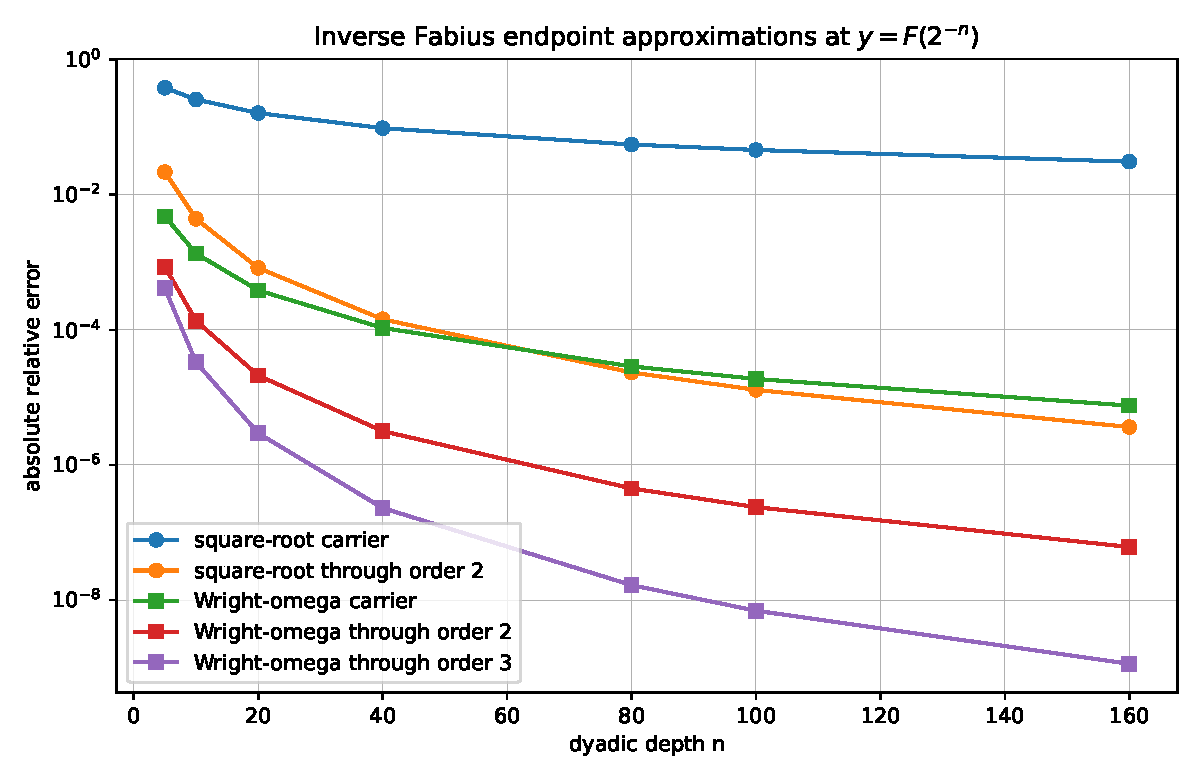
\includegraphics[width=0.78\textwidth]{assets/endpoint/wright-omega/figures/carrier_comparison.pdf}\\[0.3em]
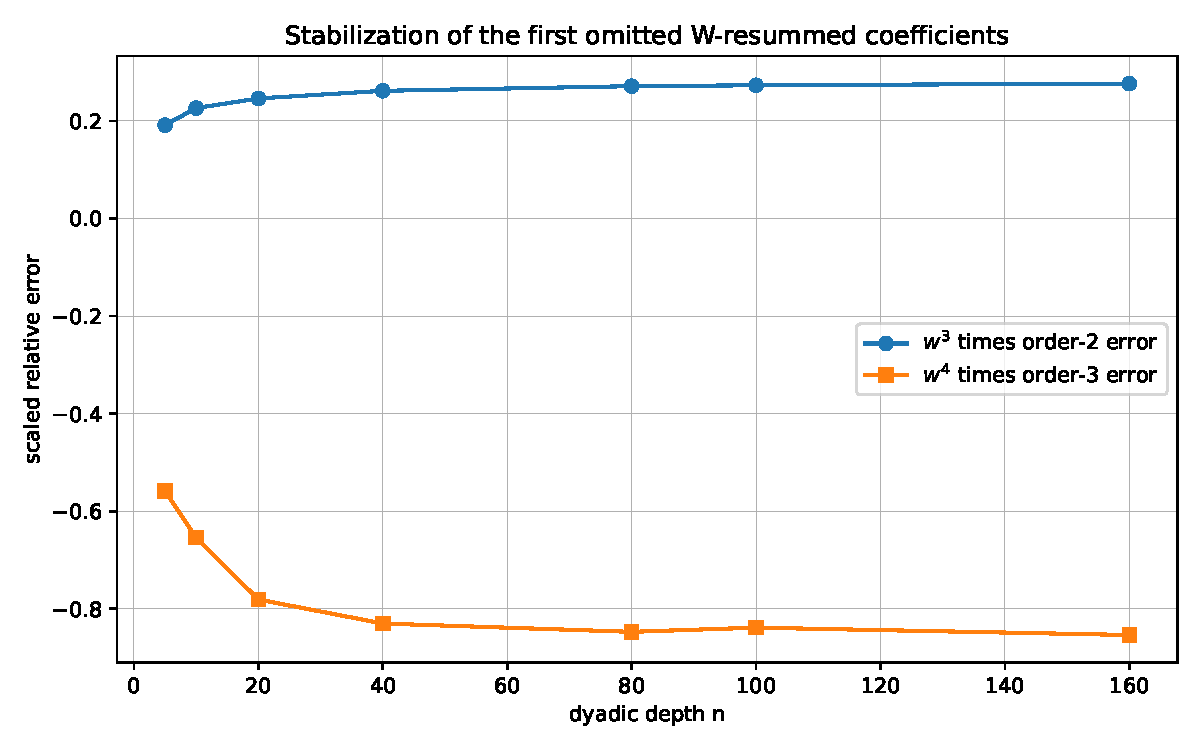
\includegraphics[width=0.78\textwidth]{assets/endpoint/wright-omega/figures/scaled_residuals.pdf}
\caption{Top: absolute relative errors of the $\rho$- and W-carrier
approximants on the exact dyadic quantiles.  Bottom: scaled residuals
after the second and third W-corrections, consistent with the
predicted next powers $w^{-3}$, $w^{-4}$.}
\label{ao:fig:W-figures}
\end{figure}

\begin{remark}[Pre-asymptotic hierarchy]
Since $\Norm{\Psi}_\infty\approx2.13\times10^{-6}$ while
$(h_2^W)^{(0)}=5/24$, the nominally first correction
$h_1^W/w=-\Psi/w$ is numerically \emph{invisible} against
$h_2^W/w^{2}$ until
$w\gtrsim(5/24)/\Norm{\Psi}_\infty\approx10^{5}$, i.e.\
$T\sim3\times10^{9}$.  Practical approximations must therefore
include $h_2^W$ whenever they include $h_1^W$
(cf.\ the table's near-identical first two columns).  This does not
violate asymptotic ordering; one coefficient simply happens to be
extraordinarily small --- the same smallness that makes the phase
oscillation resolvable only at high precision.
\end{remark}

\begin{remark}[Candidate beyond-all-orders scales; heuristic only]
The exact dyadic tail suggests an inverse perturbation on the scale
$w^{-1}e^{-2^{q_\star}}$, where $q_\star$ is the exact saddle coordinate;
replacing it by $\vartheta$ is not uniform, as explained after
\eqref{ao:eq:touchard-jets}.  A second candidate comes from the isolated
linear top-jet contribution \eqref{ao:eq:amplitude-law}.  Combining its
$k$th Fourier factor with
$|\Psihat(k)|$ and optimizing in $k$ places the largest term of that
\emph{single contribution} near
$k_*\sim2(m-1)L/\pi^2$ and suggests the factorial scale
$m!(8/\pi^2)^m$, least term near $m\sim\pi^2w/8$, and exponential size
$e^{-\pi^2w/8}$.

None of these optimizations controls the remaining saddle diagrams.  They may
reinforce or cancel the isolated Fourier mode, and no analytic continuation
of the Borel transform is proved here.  In particular this calculation does
\emph{not} establish an exact limsup, Borel summability, a Borel singularity
at $\pi^2/8$, or a Stokes multiplier.  It records only the candidate constants
used to formulate \cref{ao:conj:gevrey,ao:conj:optimal-truncation,ao:conj:transseries}.
Locating the nearest complex singularity of the bare implicit germ
\eqref{ao:eq:bare-series} is a separate elimination problem and would measure
the carrier's geometric, rather than factorial, coefficient growth.
\end{remark}

\section{The forward saddle engine: constrained partition sums}
\label{ao:sec:saddle}

The inverse formulas consume the periodic forward coefficients
$A_j$.  This chapter closes their construction with a finite
partition formula for the universal Gaussian layer of the saddle
analysis of the Bromwich integral.

Let $s>0$ solve the saddle equation $x=-K'(s)$ and normalize the
saddle jets and their ratios
\begin{equation}
 \varkappa_r=s^{r}K^{(r)}(s),
 \qquad
 \varrho_r=\frac{\varkappa_r}{\varkappa_2}
 \quad(r\ge3).
 \label{ao:eq:saddle-jets}
\end{equation}
Scaling the contour by $t=s(1+\ImaginaryUnit Z/\sqrt{\varkappa_2})$,
$Z\sim N(0,1)$, produces the formal correction factor
\begin{equation}
 \mathcal S=\Expectation\left[
 \Bigl(1+\frac{\ImaginaryUnit Z}{\sqrt{\varkappa_2}}\Bigr)^{-1}
 \exp\Bigl(\sum_{r\ge3}\frac{\varrho_r}{r!}
 \frac{(\ImaginaryUnit Z)^{r}}{\varkappa_2^{(r-2)/2}}\Bigr)
 \right]
 \sim1+\sum_{n\ge1}\frac{C_n}{\varkappa_2^{\,n}},
 \label{ao:eq:S-def}
\end{equation}
the reciprocal factor being the CDF's Bromwich $1/t$ --- deleting it
would produce the \emph{density} coefficients instead.

\begin{theorem}[Constrained-partition formula]
\label{ao:thm:Cn}
For $n\ge1$,
\begin{equation}
 \boxed{\;
 C_n=\sum_{\substack{m_0,m_3,m_4,\dots\ge0\\
 m_0+\sum_{r\ge3}(r-2)m_r=2n}}
 (-1)^{m_0+N/2}\,(N-1)!!\,
 \prod_{r\ge3}\frac{\varrho_r^{\,m_r}}{m_r!\,(r!)^{m_r}},
 \qquad
 N:=m_0+\sum_{r\ge3}rm_r,
 \;}
 \label{ao:eq:Cn-partition}
\end{equation}
a finite sum (the constraint forces $N$ even and $r\le2n+2$).  When
all $\varrho_r$ vanish it reduces to the Gaussian Mills-ratio
coefficients $C_n=(-1)^{n}(2n-1)!!$ --- a sensitive sign and
normalization check, verified symbolically ($-1,3,-15$).  The
logarithmic coefficients
$\log\mathcal S\sim\sum\Lambda_n\varkappa_2^{-n}$ follow
nonrecursively from
\begin{equation}
 \Lambda_n=\sum_{k=1}^{n}\frac{(-1)^{k-1}}k
 \sum_{n_1+\dots+n_k=n,\;n_j\ge1}
 C_{n_1}\cdots C_{n_k},
 \qquad
 \Lambda_1=C_1,\quad
 \Lambda_2=C_2-\tfrac12C_1^{2}.
 \label{ao:eq:Lambda}
\end{equation}
\end{theorem}

\begin{proof}
Expand the reciprocal geometrically ($m_0$ factors of
$-\ImaginaryUnit Z/\sqrt{\varkappa_2}$) and the exponential by multiplicities
$m_r$.  The total inverse half-power of $\varkappa_2$ is
$\tfrac12(m_0+\sum(r-2)m_r)$, giving the constraint; the Gaussian
degree is $N$ with $N-2n=2\sum m_r$ even, so
$\Expectation Z^{N}=(N-1)!!$; the powers of $\ImaginaryUnit$ and the reciprocal's sign
give $(-1)^{m_0+N/2}$; and the exponential series supplies the
multiplicity factorials.  The $\Lambda$ formula is
$\log(1+\cdot)$ composed with the $C$-series.
\end{proof}

The first coefficients are
$C_1=-1-\tfrac12\varrho_3+\tfrac18\varrho_4
-\tfrac5{24}\varrho_3^{2}$ and
\begin{equation}
 C_2=3+\tfrac52\varrho_3-\tfrac58\varrho_4+\tfrac18\varrho_5
 -\tfrac1{48}\varrho_6
 +\tfrac{35}{24}\varrho_3^{2}-\tfrac{35}{48}\varrho_3\varrho_4
 +\tfrac7{48}\varrho_3\varrho_5+\tfrac{35}{384}\varrho_4^{2}
 +\tfrac{35}{48}\varrho_3^{3}
 -\tfrac{35}{64}\varrho_3^{2}\varrho_4
 +\tfrac{385}{1152}\varrho_3^{4}.
 \label{ao:eq:C2}
\end{equation}
With $q=\log_2s$ and $J(q)=K(2^{q})$, the normalized jets are
generated exactly by the operator identity
$\varkappa_r(q)=L^{-r}\prod_{j=0}^{r-1}(D_q-jL)\,J(q)$; inserting
the exact decomposition of $K$ from
\cref{ao:sec:dyadic-completion} and converting from the saddle
coordinate $q$ to the exact Lambert phase completes the pipeline
\begin{equation}
 \Psi
 \;\longrightarrow\;\{\varkappa_r\}
 \;\xrightarrow{\eqref{ao:eq:Cn-partition}}\;\{C_n\}
 \;\xrightarrow{\eqref{ao:eq:Lambda}}\;\{\Lambda_n\}
 \;\longrightarrow\;\{A_j\}
 \;\xrightarrow{\eqref{ao:eq:diagonal-dn}}\;\{d_n\}
 \;\xrightarrow{\eqref{ao:eq:gn-direct}}\;\{g_n\},
 \label{ao:eq:pipeline}
\end{equation}
every arrow a finite differential-polynomial or
coefficient-extraction operation at fixed order.  The raw term count
of \eqref{ao:eq:Cn-partition} grows like an integer-partition function
--- subexponentially --- rather than like all set partitions, which
removes the practical bottleneck to generating $A_3,A_4,\dots$ in
compact Fourier-differential form.

For implementers, the corpus also supplies a second, fully unrolled
closed route to the same $A_j$ (recorded in the third absorbed
source from the archived small-argument study): with the signed
Stirling coefficients $\prod_{r=1}^{n}(z-r)=\sum_mc(n,m)z^{m}$ and
harmonic numbers $\Hnum_n$, the bounded saddle jets are
\begin{equation}
 q_n(u)=(-1)^{n}n!\Bigl(\frac{\Hnum_n}{L}-\frac12\Bigr)
 +\sum_{m=0}^{n}c(n,m)\,\frac{\Psi^{(m+1)}(u)}{L^{m+1}},
 \label{ao:eq:qn-jets}
\end{equation}
the normalized mass coefficients $a_j$ are finite sums over
compositions of $2j$ and subsets weighted by double factorials
$(2j+2\AbsoluteValue S-1)!!$, and
$A_j=\sum_{r\le j}\frac{(-1)^{r-1}}r
\sum_{\mathcal C(j,r)}a_{s_1}\cdots a_{s_r}$ --- an explicit finite
differential polynomial in $\Psi',\dots,\Psi^{(2j)}$ whose top jet
reproduces \eqref{ao:eq:A1-and-topjet}.  The partition engine
\eqref{ao:eq:Cn-partition} and this composition route validate each
other symbolically.

\section{The exact \texorpdfstring{$2$}{2}-adic completion of the
Laplace exponent}
\label{ao:sec:dyadic-completion}

Everything so far is asymptotic in $\rho$.  This chapter is
\emph{exact}: it completes the quadratic--periodic normal form of
$K$ by an explicitly $2$-adic, everywhere-convergent tail, and shows
that the periodic phase and the beyond-all-orders sectors are two
faces of one Mellin kernel.

\subsection{The decomposition and the dyadic Bose tail}

The product \eqref{ao:eq:K-def} gives the dyadic difference equation
$K(2t)-K(t)=\log(1-\EulerE^{-t})-\log t$.  Define the \emph{dyadic Bose
tail}
\begin{equation}
 B(t)=-\sum_{k\ge0}\log\bigl(1-\EulerE^{-2^{k}t}\bigr),
 \qquad
 B(t)=-\log(1-\EulerE^{-t})+B(2t).
 \label{ao:eq:B-def}
\end{equation}

\begin{theorem}[Exact quadratic--periodic--dyadic decomposition]
\label{ao:thm:K-decomposition}
For every $t>0$,
\begin{equation}
 \boxed{\;
 K(t)=-\frac{\log^{2}t}{2L}+\frac12\log t-\CB
 +\Psi(\log_2t)+B(t).
 \;}
 \label{ao:eq:K-decomposition}
\end{equation}
\end{theorem}

\begin{proof}
With $Q(q)=-\tfrac L2q^{2}+\tfrac L2q$ one checks
$Q(q+1)-Q(q)=-Lq$, so
$\Omega(q):=K(2^{q})-Q(q)-B(2^{q})$ is $1$-periodic by the two
difference equations.  The small-$t$ Mellin expansion of $B$
(\cref{ao:thm:mellin-bridge} below) is
$B(t)=\log^{2}(1/t)/(2L)+\tfrac12\log(1/t)+\CB-\Psi(\log_2t)+
\LittleO(1)$, and $K(t)\to0$ as $t\downarrow0$; letting
$q=m+u\to-\infty$ at fixed $u$ identifies
$\Omega(u)=\Psi(u)-\CB$, and periodicity upgrades the identity to
all $q$.
\end{proof}

\begin{theorem}[Exact $2$-adic coefficients]
\label{ao:thm:B-2adic}
For every $t>0$,
\begin{equation}
 \boxed{\;
 B(t)=\sum_{n\ge1}b_n\,\EulerE^{-nt},
 \qquad
 b_n=\frac{2^{\TwoAdicValuation(n)+1}-1}{n},
 \;}
 \qquad
 0<b_n<2,
 \label{ao:eq:B-2adic}
\end{equation}
with the elementary tail enclosure
$0<B(t)-\sum_{n\le N}b_n\EulerE^{-nt}\le2\EulerE^{-(N+1)t}/(1-\EulerE^{-t})$.
\end{theorem}

\begin{proof}
Expand each Bose logarithm and regroup
$B(t)=\sum_{k\ge0}\sum_{m\ge1}m^{-1}\EulerE^{-m2^{k}t}$: the
representations $n=m2^{k}$ are indexed by $0\le k\le\TwoAdicValuation(n)$, with
total weight
$\tfrac1n\sum_{k\le\TwoAdicValuation(n)}2^{k}=(2^{\TwoAdicValuation(n)+1}-1)/n$.
\end{proof}

The first terms,
$B(t)=\EulerE^{-t}+\tfrac32\EulerE^{-2t}+\tfrac13\EulerE^{-3t}
+\tfrac74\EulerE^{-4t}+\tfrac15\EulerE^{-5t}+\tfrac12\EulerE^{-6t}+\cdots$, spike at
powers of two: the exact arithmetic trace of the dyadic scale
hierarchy.  The integer weight $f(n)=nb_n=2^{\TwoAdicValuation(n)+1}-1$
satisfies $f(2n)=2f(n)+1$, $f(2n+1)=1$, and its generating function
obeys the Mahler equation $C(z)=2C(z^{2})+z/(1-z)$, placing the
sectors in the same digital universe as the Thue--Morse and ruler
sequences --- but with geometric accumulation over the full
$2$-adic valuation in place of digit-sum parity.  Note the
crosswalk: $\TwoAdicValuation(n)+1$ is precisely the integer zero order of
$\FourierTwoPi{\RvachevUp}$ that drives the exactness theorems of the companion
volume \emph{Dyadic-Comb Frontiers}; here the same statistic returns
as the arithmetic seed of the beyond-all-orders sectors.

\subsection{One Mellin kernel, two asymptotic ends}

\begin{theorem}[Mellin bridge]
\label{ao:thm:mellin-bridge}
For $\Re s>0$,
\begin{equation}
 \sum_{n\ge1}\frac{b_n}{n^{s}}
 =\frac{\zeta(s+1)}{1-2^{-s}},
 \qquad
 \int_0^\infty B(t)\,t^{s-1}\Differential t
 =\Gamma(s)\,\frac{\zeta(s+1)}{1-2^{-s}},
 \label{ao:eq:mellin}
\end{equation}
and contour shifting in the Mellin inversion gives, for every fixed integer
$M\ge1$, with $R=\log(1/t)$,
\begin{equation}
 B(t)=\frac{R^{2}}{2L}+\frac R2+\CB-\Psi(\log_2t)
 +\sum_{m=1}^{M-1}\frac{(-1)^{m}\zeta(1-m)}{m!\,(1-2^{m})}\,t^{m}
 +\BigO_M(t^{M})
 \qquad(t\downarrow0).
 \label{ao:eq:B-small-t}
\end{equation}
\end{theorem}

\begin{proof}
For $\Re s>0$, Tonelli's theorem applied to absolute values gives
\[
 \sum_{n\ge1}\frac{b_n}{n^s}
 =\sum_{k\ge0}\sum_{m\ge1}\frac{1}{m(m2^k)^s}
 =\zeta(s+1)\sum_{k\ge0}2^{-ks}
 =\frac{\zeta(s+1)}{1-2^{-s}}.
\]
The exact series \eqref{ao:eq:B-2adic} is locally uniformly convergent for
$t>0$.  A second application of Tonelli, followed by
$\int_0^\infty e^{-nt}t^{s-1}\,dt=n^{-s}\Gamma(s)$, proves the Mellin
transform identity.  To make the endpoint bounds explicit, put
$J=\Ceiling{\log_2(1/t)}$ when $0<t\le1$.  For $k\le J$,
$-\log(1-e^{-2^kt})\le C+|\log(2^kt)|$, whose sum is
$O((1+|\log t|)^2)$; for $k>J$, the inequality
$-\log(1-e^{-u})\le C e^{-u}$ for $u\ge1$ and dyadic growth give a bounded
tail.  Thus $B(t)$ has at most quadratic logarithmic growth at zero.  Its
defining series also gives exponential decay at infinity, so Mellin inversion
is valid on every line $\Re s=c>0$:
\[
 B(t)=\frac{1}{2\pi\ImaginaryUnit}
 \int_{c-\ImaginaryUnit\infty}^{c+\ImaginaryUnit\infty}
 \Gamma(s)\frac{\zeta(s+1)}{1-2^{-s}}t^{-s}\,\Differential s.
\]

Shift a rectangular contour to $\Re s=-M-\tfrac12$, choosing its horizontal
edges between the poles on $\Re s=0$.  Stirling's bound gives exponential
decay $e^{-\pi|\Im s|/2}$ for $\Gamma(s)$, whereas $\zeta(s+1)$ has only
polynomial vertical growth.  Thus the horizontal integrals vanish and the
residue series on $\Re s=0$ converges normally.  The pole at $s=0$ has order
three.  The Laurent expansions
\[
 \Gamma(s)=\frac1s-\gamma+
 \left(\frac{\gamma^2}{2}+\frac{\pi^2}{12}\right)s+O(s^2),\qquad
 \zeta(1+s)=\frac1s+\gamma-\gamma_1s+O(s^2),
\]
\[
 \frac1{1-e^{-Ls}}=\frac1{Ls}+\frac12+\frac{Ls}{12}+O(s^3),
 \qquad t^{-s}=e^{Rs}=1+Rs+\frac{R^2s^2}{2}+O(s^3)
\]
show that its residue contribution is
\[
 \frac{R^2}{2L}+\frac R2+\frac L{12}
 +\frac{\pi^2-6\gamma^2-12\gamma_1}{12L}
 =\frac{R^2}{2L}+\frac R2+\CB.
\]
The other zeros of $1-2^{-s}$ are the simple points $s=\chi_k$, $k\ne0$.
Their residues sum, after replacing $k$ by $-k$, to
\[
 \sum_{k\ne0}\frac{\Gamma(-\chi_k)\zeta(1-\chi_k)}{L}t^{\chi_k}
 =-\Psi(\log_2t).
\]
At $s=-m$, $1\le m\le M$, the residue of $\Gamma$ is $(-1)^m/m!$,
so the corresponding term is
\[
 \frac{(-1)^m\zeta(1-m)}{m!(1-2^m)}t^m.
\]
On the new vertical line the denominator is bounded away from zero, and the
same Gamma estimate bounds the remaining integral by $O_M(t^{M+1/2})$.
Retain the residues with $m<M$ and absorb the $m=M$ term and the new-line
integral into $O_M(t^M)$.  This proves \eqref{ao:eq:B-small-t}.
\end{proof}

\begin{statuspanel}{Two faces of one kernel}
The Gamma--zeta phase $\Psi$ (small-$t$ residues at the complex
dimensions $2\pi\ImaginaryUnit k/L$) and the exact $2$-adic exponential sectors
(large-$t$ Dirichlet regrouping) are generated by the \emph{same}
kernel $\Gamma(s)\zeta(s+1)/(1-2^{-s})$.  No new frequencies ever
appear downstream: the entire hierarchy of inverse oscillations
consists of integer convolutions of the modes
$\chi_k$ (\cref{ao:prop:convolutions}), and the beyond-all-orders
remainder is not an opaque error but the explicit arithmetic object
\eqref{ao:eq:B-2adic}.  Comparing the two constant terms independently
recovers the relation $\Csharp+\CB=-\tfrac12\log(2\pi)$ already visible in
\eqref{ao:eq:constants}.
\end{statuspanel}

\subsection{Exact saddle map and ultraflat jets}

\begin{corollary}[Exact $2$-adic saddle map]
\label{ao:cor:saddle-map}
With $t=2^{q}$, the saddle abscissa $x=-K'(t)$ is exactly
\begin{equation}
 \boxed{\;
 x(q)=2^{-q}\Bigl(q-\frac12-\frac{\Psi'(q)}{L}\Bigr)
 +\sum_{n\ge1}\bigl(2^{\TwoAdicValuation(n)+1}-1\bigr)\,\EulerE^{-n2^{q}},
 \;}
 \label{ao:eq:saddle-map}
\end{equation}
the first term the complete algebraic--periodic saddle map, the
second an exact convergent ultraflat correction.  Derivative
bookkeeping is closed: with Stirling numbers of the second kind,
\begin{equation}
 \frac{\Differential^{r}}{\Differential q^{r}}B(2^{q})
 =L^{r}\sum_{n\ge1}b_n
 \sum_{j=0}^{r}
 \genfrac\{\}{0pt}{}{r}{j}\,(-n2^{q})^{j}\,\EulerE^{-n2^{q}},
 \qquad
 t^{r}B^{(r)}(t)=(-1)^{r}\sum_{n\ge1}b_n\,(nt)^{r}\EulerE^{-nt}.
 \label{ao:eq:touchard-jets}
\end{equation}
\end{corollary}

\begin{proof}
Differentiate the exact decomposition \eqref{ao:eq:K-decomposition}.  Since
$q=\log_2t=(\log t)/L$,
\[
 -K'(t)=\frac1t\left(q-\frac12-\frac{\Psi'(q)}L\right)-B'(t).
\]
The series in \eqref{ao:eq:B-2adic} and all of its termwise derivatives
converge uniformly on each half-line $t\ge t_0>0$, so
\[
 -B'(t)=\sum_{n\ge1}n b_ne^{-nt}
 =\sum_{n\ge1}(2^{\TwoAdicValuation(n)+1}-1)e^{-nt}.
\]
Putting $t=2^q$ gives \eqref{ao:eq:saddle-map}.

Ordinary termwise differentiation gives
\[
 t^rB^{(r)}(t)=(-1)^r\sum_{n\ge1}b_n(nt)^re^{-nt}.
\]
For derivatives in $q$, use
$\Differential/\Differential q=L,t\Differential/\Differential t$ and the
operator identity
\[
 (t\Differential_t)^r
 =\sum_{j=0}^r\genfrac\{\}{0pt}{}{r}{j}t^j\Differential_t^j.
\]
Applying it termwise to $e^{-nt}$ proves the first formula in
\eqref{ao:eq:touchard-jets}.  Uniform convergence on compact $q$-intervals
justifies all differentiations and interchanges.
\end{proof}

The jet formulas expose the technical obstacle to naive
hyperasymptotics: each $q$-derivative of an
$\EulerE^{-n2^{q}}$ sector produces powers of $2^{q}$, so the ordinary
inverse-power saddle hierarchy is \emph{not uniform} inside a fixed
dyadic sector; and although the algebraic inversion gives the saddle
coordinate $q_\star(y)=\theta+\BigO(\ell/\rho)$, the induced change
in the exponent $n2^{q_\star}$ is of order
$2^{\theta}\ell/\rho\to\infty$ --- the exact saddle coordinate is
part of the beyond-all-orders datum
(\cref{ao:conj:transseries}).

% Source fragment: All-orders endpoint asymptotics; prefix ao.
\section{Verification}
\label{ao:sec:verification-inv}

The two absorbed packages verify overlapping claims by independent
implementations; both suites live under \nolinkurl{assets/}.

\emph{Symbolic.}  Over algebraically independent symbols
$L,\beta,\Csharp,\ell,P_0,\dots,P_4,A_1,A_1',A_2$, both codes confirm
$d^{\mathrm{diagonal}}_j-d^{\mathrm{triangular}}_j\equiv0$
($j\le3$), the third correction \eqref{ao:eq:d3}, the universal top-log
\eqref{ao:eq:universal-top-log}, and the top-jet transfer
\eqref{ao:eq:inverse-topjet}; the saddle generator reproduces
$C_n=(-1)^{n}(2n-1)!!$ at vanishing $\varrho$ and archives
$C_1,C_2,C_3,\Lambda_2$ (\nolinkurl{generated_coefficients.tex}).

\emph{Exact identities.}  At $70$--$100$ digits, the decomposition
\eqref{ao:eq:K-decomposition} agrees with the defining product for
$K$ to $\sim10^{-16}$ at $t\in\{0.1,1,3,10\}$ (twelve Fourier
modes); the $2$-adic series \eqref{ao:eq:B-2adic} agrees with the
product to $7.5\times10^{-39}$ at $t=0.7$ and
$3.8\times10^{-55}$ at $t=1.5$; the small-$t$ expansion
\eqref{ao:eq:B-small-t} to $\sim4\times10^{-16}$ on
$0.02\le t\le0.2$; and the Dirichlet identity
\eqref{ao:eq:mellin} to the expected algebraic truncation tail with
$5\times10^{4}$ unaccelerated terms.

\emph{Wright-omega layer.}  The third source's suite independently
reconstructs the W-scale $d_m^W,h_m^W,g_m^W$ symbolically from the residual
equation (SymPy; the identities of
\cref{ao:sec:wcarrier} including the $5/24$ cancellation and the
zero-periodic values \eqref{ao:eq:zero-periodic}), verifies the carrier
equation and Newton evaluation of $\omega$, and generates the
carrier-comparison tables of \cref{ao:tab:W-errors} on the same exact
dyadic quantiles at $100$ digits with nine Fourier modes.

\emph{Exact dyadic quantiles.}  With $a_0=1$ and
$a_n=(2^{n}-1)^{-1}\sum_{k<n}a_k/(n-k+1)!$, the repository's exact
values give $y_n=F(2^{-n})=2^{-n(n-1)/2}a_n$ with
$G(y_n)=2^{-n}$ \emph{exactly} --- no inversion error, only the
asymptotic formula is evaluated (at $100$ digits, twelve modes).
Signed relative errors of $G^{[r]}
=\Gzero\exp(\sum_{j\le r}h_j\rho^{-j})$:

\begin{center}
\small
\begin{tabular}{@{}rrrrrr@{}}
\toprule
$n$ & $\rho$ & $\Gzero$ only & through $h_1$ & through $h_2$ & through $h_3$ \\
\midrule
5   & 6.44   & $-3.83\times10^{-1}$ & $7.89\times10^{-2}$ & $-2.17\times10^{-2}$ & $6.41\times10^{-3}$ \\
10  & 12.08  & $-2.57\times10^{-1}$ & $2.69\times10^{-2}$ & $-4.40\times10^{-3}$ & $7.19\times10^{-4}$ \\
20  & 22.82  & $-1.62\times10^{-1}$ & $8.76\times10^{-3}$ & $-8.24\times10^{-4}$ & $7.40\times10^{-5}$ \\
40  & 43.65  & $-9.66\times10^{-2}$ & $2.72\times10^{-3}$ & $-1.43\times10^{-4}$ & $6.96\times10^{-6}$ \\
80  & 84.54  & $-5.53\times10^{-2}$ & $8.05\times10^{-4}$ & $-2.34\times10^{-5}$ & $6.05\times10^{-7}$ \\
120 & 125.08 & $-3.94\times10^{-2}$ & $3.88\times10^{-4}$ & $-7.92\times10^{-6}$ & $1.40\times10^{-7}$ \\
160 & 165.47 & $-3.08\times10^{-2}$ & $2.30\times10^{-4}$ & $-3.64\times10^{-6}$ & $4.92\times10^{-8}$ \\
\bottomrule
\end{tabular}
\captionof{table}{Exact-quantile tests: the new third correction
improves the two-correction error by factors $11$--$74$ across the
tested range.}
\label{ao:tab:dyadic-errors}
\end{center}

\begin{figure}[htbp]
\centering
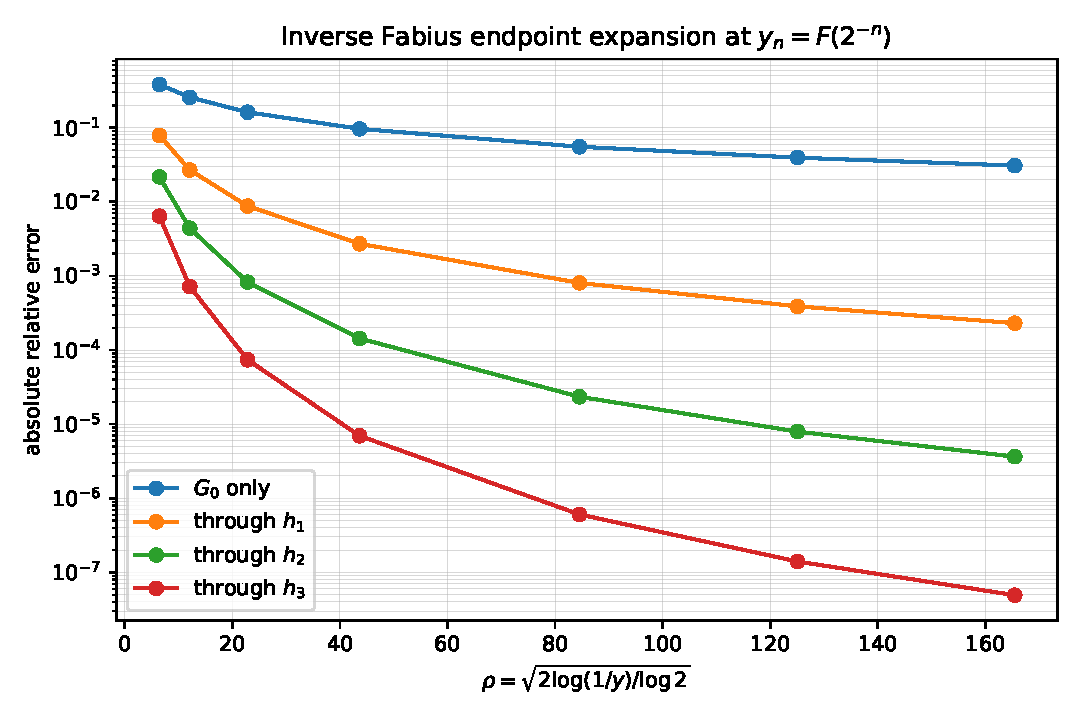
\includegraphics[width=0.78\textwidth]{assets/endpoint/all-orders/figures/endpoint_error_plot.pdf}
\caption{Absolute relative errors on the exact dyadic quantiles;
each added logarithmic correction produces the expected strong
reduction once $\rho$ is moderately large.}
\label{ao:fig:error-plot}
\end{figure}

\begin{figure}[htbp]
\centering
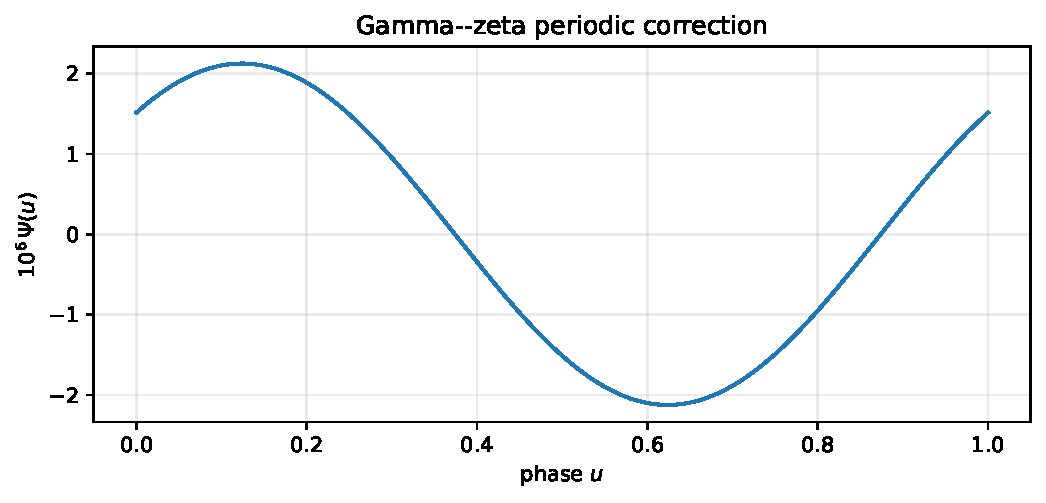
\includegraphics[width=0.72\textwidth]{assets/endpoint/dyadic-completion/figures/psi_periodic.pdf}\\[0.35em]
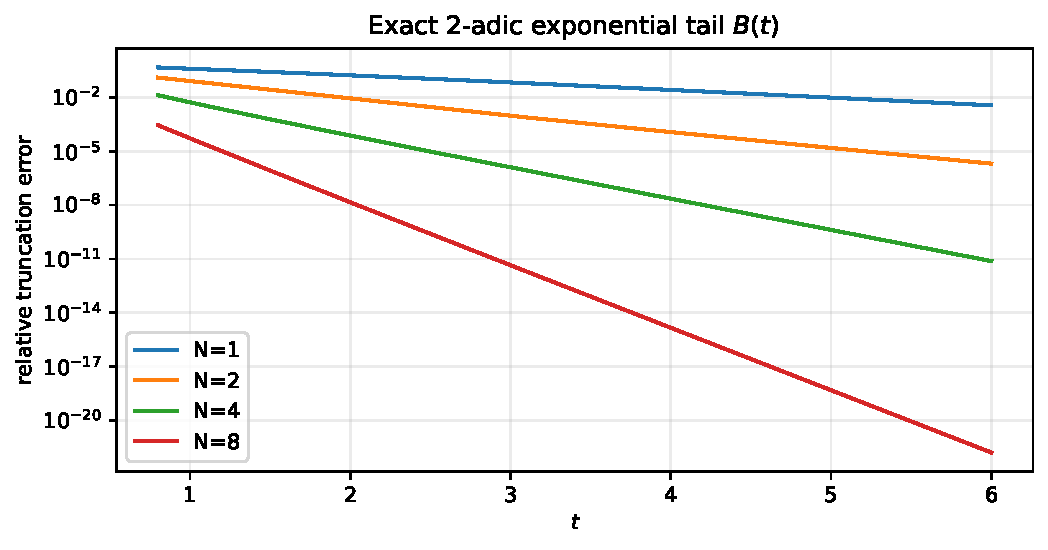
\includegraphics[width=0.72\textwidth]{assets/endpoint/dyadic-completion/figures/dyadic_tail_convergence.pdf}
\caption{Top: the centered Gamma--zeta fluctuation $\Psi$ --- tiny
amplitude, same asymptotic order as the constants.  Bottom: relative
error of $N=1,2,4,8$ terms of the exact $2$-adic series for
$B(t)$, with the elementary enclosure of
\cref{ao:thm:B-2adic}.}
\label{ao:fig:psi-and-tail}
\end{figure}

% Source fragment: All-orders endpoint asymptotics; prefix ao.
\section{Proof details}
\label{ao:app:proof-details}

\emph{Finiteness bookkeeping.}  In \eqref{ao:eq:diagonal-dn} the index-$k$
summand requests $z^{\,n-k}w^{\,k-1}$: no $\Phi$-power beyond
$z^{\,n-k}$, no Taylor jet beyond order $k-1$, and $A_j$ only for
$j\le n-k$; hence $A_{n-1}$ occurs only at $k=1$ --- the key to the
top-jet proof.

\emph{Formal-to-asymptotic transfer.}  Separate the explicit truncated
residual from the value-only error:
\[
 \mathscr F_N(w)=\frac Lz w+\mathcal R_N(w),
 \qquad \mathscr F_N(D)=-E_N(D),
 \qquad |E_N(D)|=O_N(z^N).
\]
Formal cancellation gives
$\mathscr F_N(D^{[N]})=O_N((1+\ell)^Nz^N)$, while
$\inf|\partial_w\mathscr F_N|\ge L/(2z)$ throughout the relevant
$O(\ell z)$ neighborhood.  Applying the mean-value theorem to
$\mathscr F_N$ alone gives
\[
 |D-D^{[N]}|
 \le\frac{2z}{L}
 \bigl(|E_N(D)|+|\mathscr F_N(D^{[N]})|\bigr)
 =O_N((1+\ell)^Nz^{N+1}).
\]
No derivative of $E_N$ is assumed.  This is the gain-of-one-power argument
that lets a forward expansion through $A_{N-1}$ certify an inverse
expansion through $d_N$.  The map
$\lambda\mapsto\lambda\EulerE^{-L\lambda}$ then transfers phase error to
relative inverse error of the same order.

% Source fragment: All-orders endpoint asymptotics; prefix ao.
\section{Conjectures and frontier directions}
\label{ao:sec:conjectures-inv}

\begin{conjecture}[Gevrey-one growth]
\label{ao:conj:gevrey}
For every $0<\sigma'<\pi/(2L)$ there are $C,A>0$ such that
\[
 \|d_n^W\|_{\sigma'}+\|h_n^W\|_{\sigma'}+
 \|g_n^W\|_{\sigma'}\le CA^nn!\qquad(n\ge1).
\]
Writing a $\rho$-coefficient as
$p_n(\ell,\theta)=\sum_rp_{n,r}(\theta)\ell^r$, the same estimate holds
for the coefficient norm $\max_r\|p_{n,r}\|_{\sigma'}$, for each of
$p_n=d_n,h_n,g_n$.  The calculation in the preceding heuristic suggests
$8/\pi^2$ as a candidate exponential constant for one linear contribution,
but this conjecture asserts only Gevrey order one, not that constant and not
Borel summability.
\end{conjecture}

\begin{conjecture}[Optimal truncation]
\label{ao:conj:optimal-truncation}
Fix $u\in\RealNumbers/\IntegerNumbers$ and approach the endpoint along a
W-phase-locked sequence $\vartheta\equiv u\pmod1$.  If the leading
saddle-resurgent multiplier at that phase is nonzero, then the least term of
the W-series occurs at
$N_{\mathrm{opt}}=(\pi^2/8+o(1))w$, and truncation there has relative
remainder $R_u(w)$ satisfying
\[
 \log|R_u(w)|=-\left(\frac{\pi^2}{8}+o(1)\right)w.
\]
The qualification on the multiplier allows exceptional phases at which the
first sector cancels.  No summability assertion is included.
\end{conjecture}

\begin{conjecture}[Sharp strip inheritance]
\label{ao:conj:strip-sharp}
Every nonconstant periodic coefficient occurring in
$d_n,h_n,g_n,d_n^W,h_n^W,g_n^W$ has maximal open strip
$|\Im\theta|<\pi/(2L)$, the maximal strip of $\Psi$, unless its boundary
singularities cancel by an algebraic identity.  In particular the generic
coefficient at each inverse order has Fourier exponential type exactly
$\pi^2/L$ rather than merely at least that type as proved in
\cref{ao:prop:strip}.
\end{conjecture}

\begin{conjecture}[Nonconstant phase at every order]
\label{ao:conj:nonconstant-phase}
For every $n\ge1$, at least one nonzero Fourier coefficient of each
$d_n(\ell,\cdot),h_n(\ell,\cdot),g_n(\ell,\cdot)$ is a nonzero polynomial in
$\ell$; equivalently, none of the three coefficients is phase-blind for all
$\ell$.  Likewise each of $d_n^W,h_n^W,g_n^W$ is nonconstant in its phase.
The formal top-jet law proves that these differential polynomials are not
formally constant; the remaining content is to exclude an identity after
substitution of the particular Gamma--zeta function $\Psi$.
\end{conjecture}

The geometry of the joint phase profiles---immersion, self-intersection, and
possible embeddings after several coefficients are recorded---is a separate
problem and is not part of the preceding nonconstancy conjecture.

\begin{conjecture}[Two-level exponentially improved transseries]
\label{ao:conj:transseries}
After truncating the algebraic W-series at its least term, the relative
remainder decomposes into two asymptotically distinct families.  The first is
a saddle family on scales $e^{-c_jw}$ determined by large-order asymptotics
of the forward coefficients $A_j$.  The second is an ultraflat family on the
exact scales
\[
 \exp(-n2^{q_\star(y)})\qquad(n\ge1),
\]
where $q_\star(y)$ is the exact saddle coordinate of
\eqref{ao:eq:saddle-map}, not the leading phase $\theta$.  At each fixed
ultraflat product order, its arithmetic coefficient sequence belongs to the
finite Dirichlet-convolution algebra generated by
$b_n=(2^{\TwoAdicValuation(n)+1}-1)/n$; equivalently its Dirichlet series is a
finite linear combination of products of shifted copies of
$\zeta(s+1)/(1-2^{-s})$.  The conjecture asserts this scale and coefficient
algebra, but neither Borel summability nor particular Stokes constants.
\end{conjecture}

\begin{conjecture}[Universal diagonal inversion class]
\label{ao:conj:universal-class}
Let $a>0$.  Suppose an endpoint CDF has a strictly monotone exact phase
$\lambda\to\infty$ and a forward expansion
\[
 -a\lambda^2+b\lambda-c\log\lambda+C+P(\lambda)
 +\sum_{j<N}A_j(\lambda)\lambda^{-j}+R_N(\lambda),
\]
where $P,A_j$ are periodic and holomorphic on a common strip, the remainders
and every fixed finite set of their phase derivatives are uniform, and the
phase equation has derivative $2a\lambda+O(1)$ bounded away from zero.  Then
its inverse has a unique diagonal expansion with polynomial logarithms,
phase-locked limits, and Bell conversion; the highest logarithms depend only
on $a$ and $c$.  Any newest-jet conclusion additionally requires a stated
top-jet law for the forward $A_j$.

For the separate base-$b>1$ product of uniform smoothing factors, the exact
digital tail has coefficients
$(b^{\nu_b(n)+1}-1)/((b-1)n)$, Mellin kernel
$\zeta(s+1)/(1-b^{-s})$, and period one in $\log_b$.  The conjectural part is
that the preceding analytic hypotheses and inverse package hold uniformly in
this base-$b$ family; the coefficient regrouping itself is an elementary
finite-valuation calculation.
\end{conjecture}

Concrete projects: generate $A_3,A_4$ compactly through the pipeline
\eqref{ao:eq:pipeline} and make $g_4,g_5$ explicit in $\Psi$ alone;
prove weighted Wiener-algebra bounds uniform in phase; run optimal
truncation experiments to see whether the first visible
beyond-all-orders scale is saddle-resurgent or the far smaller
dyadic one; quantify the uniform-in-$m$ breakdown of the derivative
law \eqref{ao:eq:two-term-derivative}; locate the nearest complex
critical values of $F$ (the analytic continuation radius of $G$ and
the Borel singularities); and build certified few-mode
Fourier-polynomial coefficient tables
$g_n\approx\sum_{r\le n}\sum_{\AbsoluteValue k\le K}c_{n,r,k}\ell^{r}
\EulerE^{2\pi\ImaginaryUnit k\theta}$ that, with one Newton step on the exact
functional equation, give a fast globally certified quantile
algorithm.

\begin{statuspanel}{Lean formalization roadmap}
Four layers, the first three purely formal:
(1) a two-scale coefficient ring (truncated series over
$\RealNumbers[\ell]\otimes C^\infty(\RealNumbers/\IntegerNumbers)$, closure under composition, log,
exp); (2) parameterized Lagrange inversion
$[t^{k}]W=\tfrac1k[w^{k-1}]\Phi^{k}$ and the diagonal specialization
\eqref{ao:eq:diagonal-dn}; (3) the Gaussian contraction
\eqref{ao:eq:Cn-partition} over an algebraic moment functional, and the
$2$-adic regrouping and Dirichlet identities of
\cref{ao:sec:dyadic-completion} (a bijection and two Tonelli
arguments); (4) the analytic transfer
(\cref{ao:app:proof-details}) from formal cancellation to the
fixed-order remainder.  The degree/top-jet filtrations of
\cref{ao:sec:structure} are finite combinatorics on top of (2).
\end{statuspanel}

\appendix

% Editorial bootstrap from the immutable source revision.
% This file is canonical and may be edited independently.

\part{Dyadic Self-Sampling and Alias Superconvergence}


% Source fragment: Inverse and sampling frontiers; prefix is.
\section{Normalization and established structure}
\label{is:p3:sec:background}

\subsection{The up-law, Fabius function, and Fourier convention}

Let $u=\RvachevUp$ be Rvachev's even nonnegative $C^\infty$ function supported on $[-1,1]$, normalized by
\[
 \int_{-1}^{1}u(x)\Differential x=1,
 \qquad u(0)=1.
\]
We use
\begin{equation}
 \FourierTwoPi{f}(\xi)=\int_{\RealNumbers}f(x)\EulerE^{-2\pi\iu x\xi}\Differential x,
 \qquad
 \PhiCyc(\xi)=\FourierTwoPi{u}(\xi)
 =\prod_{j=0}^{\infty}\SincPi\!\left(\frac{\xi}{2^j}\right),
 \label{is:p3:eq:Phi-product}
\end{equation}
where
\[
 \SincPi z=\begin{cases}\dfrac{\sin(\pi z)}{\pi z},&z\ne0,\\[0.4em]1,&z=0.\end{cases}
\]
The product is entire.  If $m\in\IntegerNumbers\setminus\{0\}$, then
\begin{equation}
 \OrderOperator_{\xi=m}\PhiCyc=1+\nu_2(m).
 \label{is:p3:eq:integer-multiplicity}
\end{equation}
Indeed, the factors indexed by $0\le j\le\nu_2(m)$ vanish simply and all later factors are nonzero.

This foundation is now formal rather than merely inherited from the human
corpus.  The standalone product is entire by
\path{Fabius.rvachevFourierProduct_differentiable}; for every nonzero
integer \(m\), Lean proves
\[
 \OrderOperator_{\xi=m}\PhiCyc=1+\nu_2(|m|)
\]
as \path{Fabius.analyticOrderAt_rvachevFourierProduct_int}, together with
all lower derivative vanishings and the exact nonzero leading derivative
in \path{IntegerZeroAnalyticOrder.lean}.

The standard Fabius distribution function $F:[0,1]\to[0,1]$ is related to $u$ by
\begin{equation}
 u(x)=F(1-\AbsoluteValue{x})\quad (\AbsoluteValue{x}\le1),
 \qquad
 F(t)=u(t-1)\quad(0\le t\le1).
 \label{is:p3:eq:F-up-relation}
\end{equation}
If $Y$ has density $u$, then
\begin{equation}
 \Probability(Y\le x)=F\!\left(\frac{x+1}{2}\right),
 \qquad -1\le x\le1.
 \label{is:p3:eq:centered-CDF}
\end{equation}
Thus the centered quantile is
\begin{equation}
 q(t)=2F^{-1}(t)-1.
 \label{is:p3:eq:centered-quantile}
\end{equation}

\subsection{Moments, moment generating function, and cumulants}

Write
\begin{equation}
 \mu_n=\int_{-1}^{1}x^n u(x)\Differential x,
 \qquad c_n=\mu_{2n}.
 \label{is:p3:eq:moments}
\end{equation}
Odd moments vanish.  The even moments are rational and satisfy
\begin{equation}
 (2n+1)(2^{2n}-1)c_n
 =\sum_{k=0}^{n-1}\binom{2n+1}{2k}c_k,
 \qquad c_0=1.
 \label{is:p3:eq:moment-recurrence}
\end{equation}
The moment generating function is
\begin{align}
 M(z)
 &=\int_{-1}^{1}\EulerE^{zx}u(x)\Differential x
 =\PhiCyc\!\left(\frac{\iu z}{2\pi}\right)\notag\\
 &=\prod_{j=0}^{\infty}
 \frac{\sinh(z/2^{j+1})}{z/2^{j+1}}.
 \label{is:p3:eq:mgf-product}
\end{align}
Its logarithm has even cumulants
\begin{equation}
 \log M(z)=\sum_{r=1}^{\infty}\kappa_{2r}\frac{z^{2r}}{(2r)!},
 \qquad
 \boxed{\displaystyle
 \kappa_{2r}=\frac{B_{2r}}{2r}\,
 \frac{2^{2r}}{2^{2r}-1}},
 \label{is:p3:eq:cumulants}
\end{equation}
where $B_n$ are Bernoulli numbers with $B_2=1/6$.  Consequently
\begin{equation}
 \mu_n=Y_n(0,\kappa_2,0,\kappa_4,\ldots,\kappa_n),
 \label{is:p3:eq:moment-Bell}
\end{equation}
with $Y_n$ the complete exponential Bell polynomial.

\subsection{Exact dyadic arithmetic}

For $0\le a\le2^n$, the corpus gives the finite moment--Thue--Morse formula
\begin{equation}
 F\!\left(\frac a{2^n}\right)
 =\frac{2^{-n(n+1)/2}}{n!}
 \sum_{h=0}^{a-1}\eps_h
 \sum_{k=0}^{\Floor{n/2}}
 \binom n{2k}(2a-2h-1)^{n-2k}c_k,
 \label{is:p3:eq:finite-F-moment}
\end{equation}
where $\eps_h=(-1)^{\BinaryDigitSum(h)}$.  In particular every dyadic sample of $F$ and $u$ is rational.  A second exact formula, recalled in \cref{is:p3:sec:qbinomial}, expresses the same value through Gaussian binomial coefficients at $q=1/2$ and finite signed Thue--Morse power sums.

\section{The shifted dyadic self-sampling theorem}
\label{is:p3:sec:self-sampling}

\subsection{Definition of the rules}

For $N\ge0$, $h_N=2^{-N}$, and phase $\theta\in\RealNumbers$, define
\begin{equation}
 Q_{N,\theta}[f]
 :=h_N\sum_{k\in\IntegerNumbers}
 f\bigl(h_N(k+\theta)\bigr)
 u\bigl(h_N(k+\theta)\bigr).
 \label{is:p3:eq:Q-def}
\end{equation}
Because $u$ is supported on $[-1,1]$, this is a finite sum.  The nodes are equally spaced, but the weights
\begin{equation}
 w_{N,\theta,k}=h_Nu\bigl(h_N(k+\theta)\bigr)
 \label{is:p3:eq:self-weights}
\end{equation}
are samples of the target density itself.  They are nonnegative and strictly positive at every interior node.

\begin{theorem}[Shifted self-sampling quadrature]
\label{is:p3:thm:self-sampling}
For every $N\ge0$, every $\theta\in\RealNumbers$, and every polynomial $p$ with $\deg p\le N$,
\begin{equation}
 \boxed{\displaystyle
 \int_{-1}^{1}p(x)u(x)\Differential x
 =2^{-N}\sum_{k\in\IntegerNumbers}
 p\!\left(\frac{k+\theta}{2^N}\right)
 u\!\left(\frac{k+\theta}{2^N}\right).}
 \label{is:p3:eq:self-sampling-main}
\end{equation}
In particular, $\sum_k w_{N,\theta,k}=1$, so the rule is a positive probability measure matching the first $N$ moments of $u$.
\end{theorem}

\begin{proof}
Let $0\le r\le N$ and set $f_r(x)=x^ru(x)$.  Since $u\in C_c^\infty(\RealNumbers)$, Poisson summation applies without regularization.  For the shifted lattice,
\begin{equation}
 h_N\sum_{k\in\IntegerNumbers}f_r\bigl(h_N(k+\theta)\bigr)
 =\sum_{\ell\in\IntegerNumbers}\EulerE^{2\pi\iu\ell\theta}
 \FourierTwoPi{f_r}(2^N\ell).
 \label{is:p3:eq:shifted-Poisson}
\end{equation}
Differentiating \eqref{is:p3:eq:Phi-product},
\begin{equation}
 \FourierTwoPi{f_r}(\xi)=\frac{\PhiCyc^{(r)}(\xi)}{(-2\pi\iu)^r}.
 \label{is:p3:eq:monomial-transform}
\end{equation}
The term $\ell=0$ is $\mu_r$.  If $\ell\ne0$, then \eqref{is:p3:eq:integer-multiplicity} gives
\[
 \OrderOperator_{\xi=2^N\ell}\PhiCyc
 =N+1+\nu_2(\ell)>r,
\]
so $\PhiCyc^{(r)}(2^N\ell)=0$.  Thus every nonzero alias vanishes, proving the identity for monomials and hence for all polynomials of degree at most $N$.
\end{proof}

\begin{remark}[A dyadic Strang--Fix phenomenon]
Classical Strang--Fix conditions turn zeros of a generator's Fourier transform at the dual lattice into polynomial reproduction by shifts.  Here the generator also supplies the quadrature weights.  The result is therefore a self-weighted, positive, shifted Strang--Fix rule rather than a cardinal interpolation formula.  The exact order is read directly from the $2$-adic multiplicities of the sinc product.
\end{remark}

\subsection{Rationality and denominator control}

\begin{corollary}[Positive rational rules]
\label{is:p3:cor:rational-rules}
If $\theta=a/2^s$ is dyadic, every node and every weight in \eqref{is:p3:eq:self-sampling-main} is rational.  More explicitly, with
\[
 D=N+s,
 \qquad n_k=2^sk+a,
 \qquad b_k=2^D-\AbsoluteValue{n_k},
\]
one has, whenever $\AbsoluteValue{n_k}<2^D$,
\begin{equation}
 x_k=\frac{n_k}{2^D},
 \qquad
 w_k=2^{-N}F\!\left(\frac{b_k}{2^D}\right)\in\RationalNumbers_{>0}.
 \label{is:p3:eq:rational-weights}
\end{equation}
A common denominator for all such weights is obtained by multiplying the repository's level-$D$ dyadic denominator bound by $2^N$.
\end{corollary}

\begin{proof}
Use \eqref{is:p3:eq:F-up-relation} at the dyadic node $x_k$.  The denominator assertion follows from the established bound
\[
 D!\,2^{\binom{D+1}{2}}(2\Floor{D/2}+1)!!
 \prod_{j=1}^{\Floor{D/2}}(2^{2j}-1)\,u(n/2^D)\in\NaturalNumbers
\]
for $\AbsoluteValue n<2^D$.
\end{proof}

\subsection{Finite moment identities in Fabius values}

For the centered phase $\theta=0$, symmetry yields particularly transparent formulas.  For $r\ge1$ with $2r\le N$,
\begin{equation}
 \boxed{\displaystyle
 c_r=2^{1-N-2rN}
 \sum_{j=1}^{2^N-1}(2^N-j)^{2r}
 F\!\left(\frac j{2^N}\right).}
 \label{is:p3:eq:centered-moment-F}
\end{equation}
For $r=0$, normalization reads
\begin{equation}
 1=2^{-N}\left(1+2\sum_{j=1}^{2^N-1}F\!\left(\frac j{2^N}\right)\right).
 \label{is:p3:eq:centered-normalization-F}
\end{equation}
These are positive finite identities: the moment on the left is reconstructed from values of the Fabius function with no alternating coefficients.

\begin{proof}
Apply \cref{is:p3:thm:self-sampling} to $p(x)=x^{2r}$.  Pair the nodes $\pm k/2^N$, use $u(k/2^N)=F(1-k/2^N)$, and then put $j=2^N-k$.
\end{proof}

\begin{resultbox}[First frontier bridge]
The exact dyadic values in the corpus were previously used primarily as point evaluations, denominator data, or inputs to signed extrapolation.  Equations \eqref{is:p3:eq:self-sampling-main}--\eqref{is:p3:eq:centered-moment-F} instead organize them as a hierarchy of positive moment designs.  Fourier zero multiplicities, dyadic rationality, and probability positivity become three faces of one formula.
\end{resultbox}

\section{The master alias function and the
\texorpdfstring{$2$}{2}-adic error filtration}
\label{is:p3:sec:alias}

\subsection{An entire generating function for all moment defects}

Define
\begin{equation}
 G_{N,\theta}(z)
 :=Q_{N,\theta}[\EulerE^{zx}]-M(z).
 \label{is:p3:eq:G-def}
\end{equation}
The coefficient of $z^r/r!$ is exactly the $r$th moment defect
\begin{equation}
 E_{N,r}(\theta)
 :=Q_{N,\theta}[x^r]-\mu_r.
 \label{is:p3:eq:ENr-def}
\end{equation}

\begin{theorem}[Master shifted-alias identity]
\label{is:p3:thm:master-alias}
For every $N\ge0$, $\theta\in\RealNumbers$, and $z\in\ComplexNumbers$,
\begin{equation}
 \boxed{\displaystyle
 G_{N,\theta}(z)
 =\sum_{\ell\in\IntegerNumbers\setminus\{0\}}
 \EulerE^{2\pi\iu\ell\theta}
 \PhiCyc\!\left(2^N\ell+\frac{\iu z}{2\pi}\right).}
 \label{is:p3:eq:master-alias}
\end{equation}
The series is locally normally convergent.  Moreover $G_{N,\theta}$ has a zero of order at least $N+1$ at $z=0$.
\end{theorem}

\begin{proof}
Apply shifted Poisson summation to $f_z(x)=\EulerE^{zx}u(x)$.  Its Fourier transform is
\[
 \FourierTwoPi{f_z}(\xi)
 =\PhiCyc\!\left(\xi+\frac{\iu z}{2\pi}\right).
\]
The zero-frequency term is $M(z)$, giving \eqref{is:p3:eq:master-alias}.  Compact support and smoothness imply the local normal convergence needed to differentiate termwise.  At $z=0$, the summand indexed by $\ell\ne0$ has order
$N+1+\nu_2(\ell)$, so the full sum begins at order $N+1$.
\end{proof}

\begin{corollary}[Valuation filtration of polynomial errors]
\label{is:p3:cor:valuation-filtration}
For $r>N$,
\begin{equation}
 E_{N,r}(\theta)
 =\frac1{(-2\pi\iu)^r}
 \sum_{a=0}^{r-N-1}
 \sum_{\substack{q\in\IntegerNumbers\setminus\{0\}\\q\ \mathrm{odd}}}
 \EulerE^{2\pi\iu 2^aq\theta}
 \PhiCyc^{(r)}(2^{N+a}q).
 \label{is:p3:eq:valuation-filtration}
\end{equation}
Thus the excess degree $r-N$ exposes exactly the first $r-N$ layers of the $2$-adic alias tree.
\end{corollary}

\begin{proof}
In the coefficient formula obtained from \eqref{is:p3:eq:master-alias}, an alias $\ell$ can contribute only if
$N+1+\nu_2(\ell)\le r$.  Write $\ell=2^aq$ with $q$ odd.
\end{proof}

\begin{remark}
The first failure, $r=N+1$, sees only odd aliases.  The next failure, $r=N+2$, sees odd aliases and twice-odd aliases.  Higher defects are therefore not arbitrary: they are a triangular sequence of $2$-adic spectral layers.  This observation will be the basis of the next-defect conjectures in \cref{is:p3:sec:frontier}.
\end{remark}

\subsection{An exact local factorization at every integer zero}

The integer zero jets can be organized in a form that makes Bell polynomials appear automatically.

\begin{proposition}[Exact local factorization]
\label{is:p3:prop:local-factorization}
Let $m=2^{d-1}q\ne0$, where $q$ is odd and $d=1+\nu_2(m)$.  Then, for $w$ near $0$,
\begin{equation}
 \boxed{\displaystyle
 \PhiCyc(m+w)
 =-\left(\frac{w}{m+w}\right)^d
 \left(\prod_{j=0}^{d-1}\SincPi\!\left(\frac{w}{2^j}\right)\right)
 \PhiCyc\!\left(\frac q2+\frac{w}{2^d}\right).}
 \label{is:p3:eq:local-factorization}
\end{equation}
In particular,
\begin{equation}
 \PhiCyc(m+w)=C_mw^d
 \exp\!\left(\sum_{j\ge1}\gamma_j(m)\frac{w^j}{j!}\right),
 \qquad
 C_m=-\frac{\PhiCyc(q/2)}{m^d},
 \label{is:p3:eq:local-Bell-form}
\end{equation}
where the logarithmic jet $\gamma_j(m)$ is explicit.
\end{proposition}

\begin{proof}
For $0\le j\le d-1$, $m/2^j$ is an integer and
\[
 \SincPi\!\left(\frac{m+w}{2^j}\right)
 =(-1)^{m/2^j}\frac{w}{m+w}
 \SincPi\!\left(\frac{w}{2^j}\right).
\]
The product of the signs is $-1$ because
\[
 \sum_{j=0}^{d-1}\frac m{2^j}=q(2^d-1)
\]
is odd.  The remaining tail is
\[
 \prod_{j=d}^{\infty}\SincPi\!\left(\frac{m+w}{2^j}\right)
 =\PhiCyc\!\left(\frac q2+\frac{w}{2^d}\right).
\]
This proves \eqref{is:p3:eq:local-factorization}; taking the analytic logarithm after removing $C_mw^d$ gives \eqref{is:p3:eq:local-Bell-form}.
\end{proof}

\begin{statusbox}[Lean status of the local factorization]
Equation \eqref{is:p3:eq:local-factorization} is now formal in a stronger total,
denominator-cleared form valid for every complex \(w\), including the
removable points.  The all-nonzero-integer statement is
\path{Fabius.rvachevFourierProduct_int_add_factorization}; its divided
germ form is
\path{Fabius.rvachevFourierProduct_int_add_eventuallyEq_pow_mul_cofactor}.
The cofactor is analytic and nonzero at the local origin, so Lean proves the exact order, every
lower-jet vanishing, and the leading identity
\eqref{is:p3:eq:first-zero-jet}.  More generally, if that cofactor is denoted by
\(U_m\) and \(d=1+\nu_2(|m|)\), Lean proves every higher jet as
\[
 \PhiCyc^{(d+r)}(m)=\binom{d+r}{d}d!\,U_m^{(r)}(0)
 \qquad(r\in\NaturalNumbers)
\]
in \path{Fabius.iteratedDeriv_rvachevFourierProduct_int_add_order}.
The generic engine in \path{LeadingJet.lean} is vector-valued and computes
every derivative index over an arbitrary nontrivially normed field.  The
explicit normalization in \eqref{is:p3:eq:local-Bell-form}, the logarithmic coefficients
\eqref{is:p3:eq:gamma1}--\eqref{is:p3:eq:gamma-general} and the Bell-polynomial formula
\eqref{is:p3:eq:Bell-zero-jets} for \(s>0\) remain human-readable frontier
results, not named Lean theorems.
\end{statusbox}

The first logarithmic coefficient is especially simple:
\begin{equation}
 \gamma_1(m)=-\frac d m
 +2^{-d}\frac{\PhiCyc'(q/2)}{\PhiCyc(q/2)}.
 \label{is:p3:eq:gamma1}
\end{equation}
For general $j$,
\begin{equation}
 \gamma_j(m)
 =d(-1)^j\frac{(j-1)!}{m^j}
 +\sum_{h=0}^{d-1}2^{-hj}\ell_j
 +2^{-dj}L_j(q/2),
 \label{is:p3:eq:gamma-general}
\end{equation}
where
\[
 \ell_j=\left.\frac{\Differential^j}{\Differential z^j}\log\SincPi z\right|_{z=0},
 \qquad
 L_j(t)=\frac{\Differential^j}{\Differential t^j}\log\PhiCyc(t).
\]
The universal local coefficients satisfy
\begin{equation}
 \ell_{2r}=-\frac{(2r)!}{r}\zeta(2r),
 \qquad \ell_{2r+1}=0,
 \label{is:p3:eq:sinc-log-jet}
\end{equation}
so Bernoulli numbers may be substituted through Euler's formula for $\zeta(2r)$.

\begin{corollary}[Bell-polynomial zero jets]
\label{is:p3:cor:Bell-zero-jets}
With the notation of \cref{is:p3:prop:local-factorization}, for every $s\ge0$,
\begin{equation}
 \boxed{\displaystyle
 \PhiCyc^{(d+s)}(m)
 =C_m\frac{(d+s)!}{s!}
 Y_s\bigl(\gamma_1(m),\ldots,\gamma_s(m)\bigr).}
 \label{is:p3:eq:Bell-zero-jets}
\end{equation}
Here $Y_0=1$.  Consequently every layer of \eqref{is:p3:eq:valuation-filtration} has a finite Bell-polynomial description in half-integer logarithmic derivatives, zeta values, and elementary $2$-adic data.
\end{corollary}

\begin{proof}
Use the defining exponential generating function
\[
 \exp\!\left(\sum_{j\ge1}x_j\frac{w^j}{j!}\right)
 =\sum_{s\ge0}Y_s(x_1,\ldots,x_s)\frac{w^s}{s!}
\]
in \eqref{is:p3:eq:local-Bell-form} and compare coefficients.
\end{proof}

\begin{resultbox}[Second frontier bridge]
The corpus already contains the integer zero multiplicities and several zero-jet formulas.  The new point here is their use as an \emph{error calculus}: the excess polynomial degree selects a finite set of $2$-adic alias layers, and every derivative on those layers is generated by a complete Bell polynomial.  Bernoulli/zeta data enter locally through $\log\SincPi$, while Thue--Morse data enter globally through the half-integer tail.
\end{resultbox}

\section{The first defect: half-integer spectrum and Thue--Morse signs}
\label{is:p3:sec:first-defect}

Put
\begin{equation}
 r=N+1,
 \qquad
 E_N(\theta):=E_{N,N+1}(\theta).
 \label{is:p3:eq:first-defect-def}
\end{equation}
Only odd aliases survive.

\begin{theorem}[Exact first-defect series]
\label{is:p3:thm:first-defect}
For every $N\ge0$ and $\theta\in\RealNumbers$,
\begin{equation}
 \boxed{\displaystyle
 E_N(\theta)
 =-\frac{r!}{(-2\pi\iu)^r2^{Nr}}
 \sum_{\substack{\ell\in\IntegerNumbers\setminus\{0\}\\\ell\ \mathrm{odd}}}
 \frac{\PhiCyc(\ell/2)}{\ell^r}
 \EulerE^{2\pi\iu\ell\theta}.}
 \label{is:p3:eq:first-defect-complex}
\end{equation}
Equivalently, if $r=2s$,
\begin{equation}
 E_N(\theta)
 =\frac{2(-1)^{s+1}r!}{(2\pi)^r2^{Nr}}
 \sum_{\substack{m\ge1\\m\ \mathrm{odd}}}
 \frac{\PhiCyc(m/2)}{m^r}\cos(2\pi m\theta),
 \label{is:p3:eq:first-defect-even}
\end{equation}
and if $r=2s+1$,
\begin{equation}
 E_N(\theta)
 =\frac{2(-1)^sr!}{(2\pi)^r2^{Nr}}
 \sum_{\substack{m\ge1\\m\ \mathrm{odd}}}
 \frac{\PhiCyc(m/2)}{m^r}\sin(2\pi m\theta).
 \label{is:p3:eq:first-defect-odd}
\end{equation}
\end{theorem}

\begin{proof}
For $m=2^N\ell$ with $\ell$ odd, \cref{is:p3:prop:local-factorization} with $d=r$ gives
\begin{equation}
 \PhiCyc^{(r)}(2^N\ell)
 =-\frac{r!\PhiCyc(\ell/2)}{(2^N\ell)^r}.
 \label{is:p3:eq:first-zero-jet}
\end{equation}
Insert this into \eqref{is:p3:eq:valuation-filtration}.  Pair positive and negative odd frequencies to obtain the real forms.
\end{proof}

\subsection{The spectral sign is exactly Thue--Morse}

\begin{proposition}[Half-integer sign law]
\label{is:p3:prop:half-integer-sign}
For $j\ge0$,
\begin{equation}
 \Sign\PhiCyc\!\left(\frac{2j+1}{2}\right)
 =(-1)^{\BinaryDigitSum(j)}=\eps_j.
 \label{is:p3:eq:half-integer-sign}
\end{equation}
Hence the first quadrature defect is a Thue--Morse-signed half-integer spectral Dirichlet series.
\end{proposition}

\begin{proof}
On the positive real axis, $\PhiCyc$ changes sign whenever an integer zero has odd multiplicity.  At the point $(2j+1)/2=j+1/2$, the total number of zero crossings, counted with multiplicity, is
\[
 \sum_{m=1}^{j}\bigl(1+\nu_2(m)\bigr)
 =j+\nu_2(j!)
 =2j-\BinaryDigitSum(j),
\]
where the last equality is Legendre's formula
$\nu_2(j!)=j-\BinaryDigitSum(j)$.  Its parity is therefore
$\BinaryDigitSum(j)$.  Since $\PhiCyc(1/2)>0$, the claimed sign follows.
\end{proof}

Writing
\begin{equation}
 a_j=\AbsoluteValue{\PhiCyc((2j+1)/2)},
 \label{is:p3:eq:half-amplitudes}
\end{equation}
we may rewrite the spectral coefficient as $\PhiCyc((2j+1)/2)=\eps_ja_j$.  Thus the signs are purely digital, while the amplitudes record the sinc-product decay.

\subsection{Symmetries}

\begin{corollary}[Phase symmetries]
\label{is:p3:cor:defect-symmetries}
The first defect is $1$-periodic and satisfies
\begin{equation}
 E_N(-\theta)=(-1)^rE_N(\theta),
 \qquad
 E_N(\theta+1/2)=-E_N(\theta).
 \label{is:p3:eq:defect-symmetries}
\end{equation}
\end{corollary}

\begin{proof}
The first identity follows from the sine/cosine parity.  The second follows because every frequency in \eqref{is:p3:eq:first-defect-complex} is odd.
\end{proof}

\section{A Bernoulli convolution formula for the first defect}
\label{is:p3:sec:bernoulli-kernel}

\subsection{The periodic up-kernel}

Define a $1$-periodic continuous function $\Kcal$ by
\begin{equation}
 \Kcal(t)=2u(2t)-1,
 \qquad -\frac12\le t\le\frac12,
 \label{is:p3:eq:K-kernel}
\end{equation}
with periodic extension.  Its mean is zero.  For $n\ne0$, its Fourier coefficient is
\begin{equation}
 \FourierSeriesCoefficient{\Kcal}{n}
 =\int_{-1/2}^{1/2}\Kcal(t)\EulerE^{-2\pi\iu nt}\Differential t
 =\PhiCyc(n/2).
 \label{is:p3:eq:K-Fourier}
\end{equation}
In particular the even nonzero coefficients vanish, and the odd coefficients carry the Thue--Morse signs of \cref{is:p3:prop:half-integer-sign}.

Let $\Bper_r(t)=B_r(\{t\})$ be the periodic Bernoulli polynomial, understood in the standard Fourier/distributional sense when $r=1$.  For $n\ne0$,
\begin{equation}
 \FourierSeriesCoefficient{\Bper_r}{n}=-\frac{r!}{(2\pi\iu n)^r}.
 \label{is:p3:eq:periodic-Bernoulli-Fourier}
\end{equation}

\begin{theorem}[Bernoulli--Rvachev error kernel]
\label{is:p3:thm:Bernoulli-convolution}
For $r=N+1$,
\begin{equation}
 \boxed{\displaystyle
 E_N(\theta)=(-1)^r2^{-Nr}
 (\Bper_r*\Kcal)(\theta),}
 \label{is:p3:eq:Bernoulli-convolution}
\end{equation}
where convolution is on $\RealNumbers/\IntegerNumbers$.
\end{theorem}

\begin{proof}
Multiply the nonzero Fourier coefficients in \eqref{is:p3:eq:K-Fourier} and \eqref{is:p3:eq:periodic-Bernoulli-Fourier}.  The resulting Fourier series is exactly \eqref{is:p3:eq:first-defect-complex}; the even frequencies vanish automatically.
\end{proof}

\begin{remark}
This formula is not an Euler--Maclaurin expansion with an unspecified remainder.  It is an exact identity.  The universal periodic Bernoulli kernel describes polynomial aliasing, while $\Kcal$ inserts the complete half-integer spectrum of the up-law.  It therefore provides a direct analytical bridge from Bernoulli polynomials to the Rvachev sinc product.
\end{remark}

\subsection{A rigorous first-harmonic bound}

\begin{lemma}[Finite product loss bound]
\label{is:p3:lem:finite-product-loss}
If $0\le a_j\le1$ for $0\le j\le J$, then
\begin{equation}
 \prod_{j=0}^{J}(1-a_j)\ge1-\sum_{j=0}^{J}a_j.
 \label{is:p3:eq:finite-product-loss}
\end{equation}
\end{lemma}

\begin{proof}
The assertion is equality for $J=0$.  If it holds through $J-1$, put
$S=\sum_{j=0}^{J-1}a_j$.  Multiplication by the nonnegative number
$1-a_J$ and the induction hypothesis give
\[
 \prod_{j=0}^{J}(1-a_j)
 \ge(1-S)(1-a_J)
 =1-S-a_J+Sa_J
 \ge1-S-a_J.
\]
This proves the induction step.
\end{proof}

\begin{lemma}[A uniform lower bound at the first half-integer]
\label{is:p3:lem:phi-half-lower}
\begin{equation}
 \PhiCyc(1/2)>1-\frac{\pi^2}{18}>\frac49.
 \label{is:p3:eq:phi-half-lower}
\end{equation}
\end{lemma}

\begin{proof}
For $0\le x\le1/2$, $\SincPi x\ge1-\pi^2x^2/6$.  Set
$a_j=(\pi^2/6)4^{-(j+1)}$.  All $a_j$ lie in $(0,1)$, and
\cref{is:p3:lem:finite-product-loss}, followed by passage to the limit, gives
\[
 \PhiCyc(1/2)\ge\prod_{j=0}^{\infty}(1-a_j).
\]
This product is strictly larger than $1-\sum_ja_j$.  Indeed, if
$S=\sum_{j=2}^{\infty}a_j$, another application of the finite product bound
to the tail and passage to the limit yield
\begin{align*}
 \prod_{j=0}^{\infty}(1-a_j)
 &\ge(1-a_0)(1-a_1)(1-S)\\
 &=1-a_0-a_1-S
   +a_0a_1+S(a_0+a_1-a_0a_1)\\
 &>1-a_0-a_1-S.
\end{align*}
Consequently
\[
 \PhiCyc(1/2)>1-\frac{\pi^2}{6}\sum_{j=0}^{\infty}4^{-(j+1)}
 =1-\frac{\pi^2}{18}.
\]
The final inequality follows from $\pi^2<10$.
\end{proof}

For $r\ge2$,
\begin{equation}
 \sum_{\substack{m\ge3\\m\ \mathrm{odd}}}
 \frac{\AbsoluteValue{\PhiCyc(m/2)}}{m^r}
 \le\sum_{\substack{m\ge3\\m\ \mathrm{odd}}}\frac1{m^r}
 \le\frac{\pi^2}{8}-1<\frac14.
 \label{is:p3:eq:harmonic-tail-bound}
\end{equation}
Thus the first coefficient is larger than the sum of all remaining absolute coefficients for every $r\ge2$.

\begin{theorem}[Uniform sinusoidal asymptotics]
\label{is:p3:thm:sinusoidal-asymptotics}
Let $N\ge1$, put $r=N+1$, and define
\begin{equation}
 A_{N,r}=\frac{2r!\PhiCyc(1/2)}{(2\pi)^r2^{Nr}}.
 \label{is:p3:eq:first-harmonic-amplitude}
\end{equation}
Then, uniformly in $\theta$,
\begin{align}
 E_N(\theta)
 &=(-1)^{r/2+1}A_{N,r}\cos(2\pi\theta)
 +\BigO\!\left(A_{N,r}3^{-r}\right),&&r\ \text{even},
 \label{is:p3:eq:cos-asymptotic}\\
 E_N(\theta)
 &=(-1)^{(r-1)/2}A_{N,r}\sin(2\pi\theta)
 +\BigO\!\left(A_{N,r}3^{-r}\right),&&r\ \text{odd}.
 \label{is:p3:eq:sin-asymptotic}
\end{align}
The implied constant is absolute.
\end{theorem}

\begin{proof}
Separate the frequency $m=1$ in \eqref{is:p3:eq:first-defect-even} or \eqref{is:p3:eq:first-defect-odd}.  Since $\AbsoluteValue{\PhiCyc(m/2)}\le1$ and
$\sum_{m\ge3,\,m\text{ odd}}m^{-r}=\BigO(3^{-r})$, the remaining series has the stated uniform bound.
\end{proof}

The exact numerical ratios are far smaller than the elementary majorant:
\begin{table}[H]
\centering
\caption{Absolute spectral tail divided by the first harmonic.}
\label{is:p3:tab:harmonic-tail}
% Generated by experiments.py
\begin{tabular}{@{}rrr@{}}
\toprule
$r=N+1$ & $N$ & absolute tail / first harmonic\\
\midrule
2 & 1 & $0.0099476026$\\
3 & 2 & $0.0032220116$\\
4 & 3 & $0.001055965$\\
5 & 4 & $0.00034847136$\\
6 & 5 & $0.00011546539$\\
7 & 6 & $3.835166e-5$\\
8 & 7 & $1.2756733e-5$\\
9 & 8 & $4.2468422e-6$\\
10 & 9 & $1.4145376e-6$\\
\bottomrule
\end{tabular}

\end{table}

\section{Parity-selected positive superconvergence}
\label{is:p3:sec:superconvergence}

\subsection{Forced phases}

The real forms immediately show two parity-dependent phase families.

\begin{corollary}[One extra exact degree]
\label{is:p3:cor:forced-superconvergence}
Let $N\ge0$.
\begin{enumerate}
\item If $N$ is even, then $Q_{N,0}$ and $Q_{N,1/2}$ are exact for every polynomial of degree at most $N+1$.
\item If $N$ is odd, then $Q_{N,1/4}$ and $Q_{N,3/4}$ are exact for every polynomial of degree at most $N+1$.
\end{enumerate}
All four phase families are positive; at these dyadic phases they are rational.
\end{corollary}

\begin{proof}
If $N$ is even, $r=N+1$ is odd, and every sine in \eqref{is:p3:eq:first-defect-odd} vanishes at $\theta=0,1/2$.  If $N$ is odd, $r$ is even, and every cosine in \eqref{is:p3:eq:first-defect-even} vanishes at $\theta=1/4,3/4$ because $m$ is odd.
\end{proof}

\begin{statusbox}[Lean status of parity-selected superconvergence]
\Cref{is:p3:cor:forced-superconvergence} now has an exact compiled
counterpart.  The predicate
\path{Fabius.IsRvachevSuperconvergentPhase} records the four selected
phases, and
\path{Fabius.isRvachevSuperconvergentPhase_two_pow_iff} specializes it at
the mesh $M=2^N$ to precisely the even-$N$ endpoint/midpoint pair and the
odd-$N$ quarter-phase pair above.  The physical-coordinate statement
\path{Fabius.integral_polynomial_mul_rvachevUp_eq_normalized_tsum_superconvergent}
then gives the displayed $2^{-N}$-normalized rule for every real polynomial
of degree at most $N+1$.

The positivity and rationality clauses use already compiled kernels rather
than a new classification theorem: \path{Fabius.rvachevUp_nonneg} gives
nonnegative weights,
\path{Fabius.rvachev_pos_iff_mem_Ioo} gives strict positivity at exactly the
interior nodes, and \path{Fabius.rvachevDyadic_cast}, together with the
zero-off-support theorem \path{Fabius.rvachevUp_eq_zero_iff_not_mem_Ioo},
identifies every dyadic sample with a rational value.  This finite family
matches every clause of the corollary.  It does not classify all possible
superconvergent phases or assert sharpness beyond the selected families.
\end{statusbox}

\subsection{Classification of the superconvergent phases}

The first harmonic does more than suggest the correct phases: from level two onward it proves that there are no others.

\begin{lemma}[Odd trigonometric factor bounds]
\label{is:p3:lem:odd-trig-factor}
For odd $m\ge1$ and real $x$,
\begin{equation}
 \AbsoluteValue{\sin(mx)}\le m\AbsoluteValue{\sin x},
 \qquad
 \AbsoluteValue{\cos(mx)}\le m\AbsoluteValue{\cos x}.
 \label{is:p3:eq:odd-trig-factor}
\end{equation}
\end{lemma}

\begin{proof}
The sine inequality is standard.  For the cosine inequality put $x=t+\pi/2$; because $m$ is odd, $\cos(mx)=\pm\sin(mt)$ and $\cos x=-\sin t$.
\end{proof}

\begin{theorem}[Exact phase classification]
\label{is:p3:thm:phase-classification}
For $N\ge2$, the first defect $E_N(\theta)$ vanishes modulo $1$ exactly at
\begin{equation}
 \begin{cases}
 \theta\equiv0,\,1/2\pmod1,&N\ \text{even},\\
 \theta\equiv1/4,\,3/4\pmod1,&N\ \text{odd}.
 \end{cases}
 \label{is:p3:eq:phase-classification}
\end{equation}
Consequently these are precisely the shifted self-sampling rules with degree of exactness at least $N+1$.
\end{theorem}

\begin{proof}
Here $r=N+1\ge3$.  Suppose first that $r$ is odd.  Factor $\sin(2\pi\theta)$ from \eqref{is:p3:eq:first-defect-odd}.  By \cref{is:p3:lem:odd-trig-factor}, the absolute contribution of the remaining frequencies to the bracket is at most
\[
 \sum_{\substack{m\ge3\\m\ \mathrm{odd}}}m^{1-r}
 \le\sum_{\substack{m\ge3\\m\ \mathrm{odd}}}m^{-2}
 =\frac{\pi^2}{8}-1<\frac14.
\]
The first bracket coefficient is $\PhiCyc(1/2)>4/9$, so the bracket never vanishes.  Hence the zero set is exactly $\sin(2\pi\theta)=0$.

If $r$ is even, factor $\cos(2\pi\theta)$ and use the cosine bound in the same way.  The bracket again has a fixed nonzero sign, so its only zeros are those of $\cos(2\pi\theta)$.
\end{proof}

\begin{figure}[H]
\centering
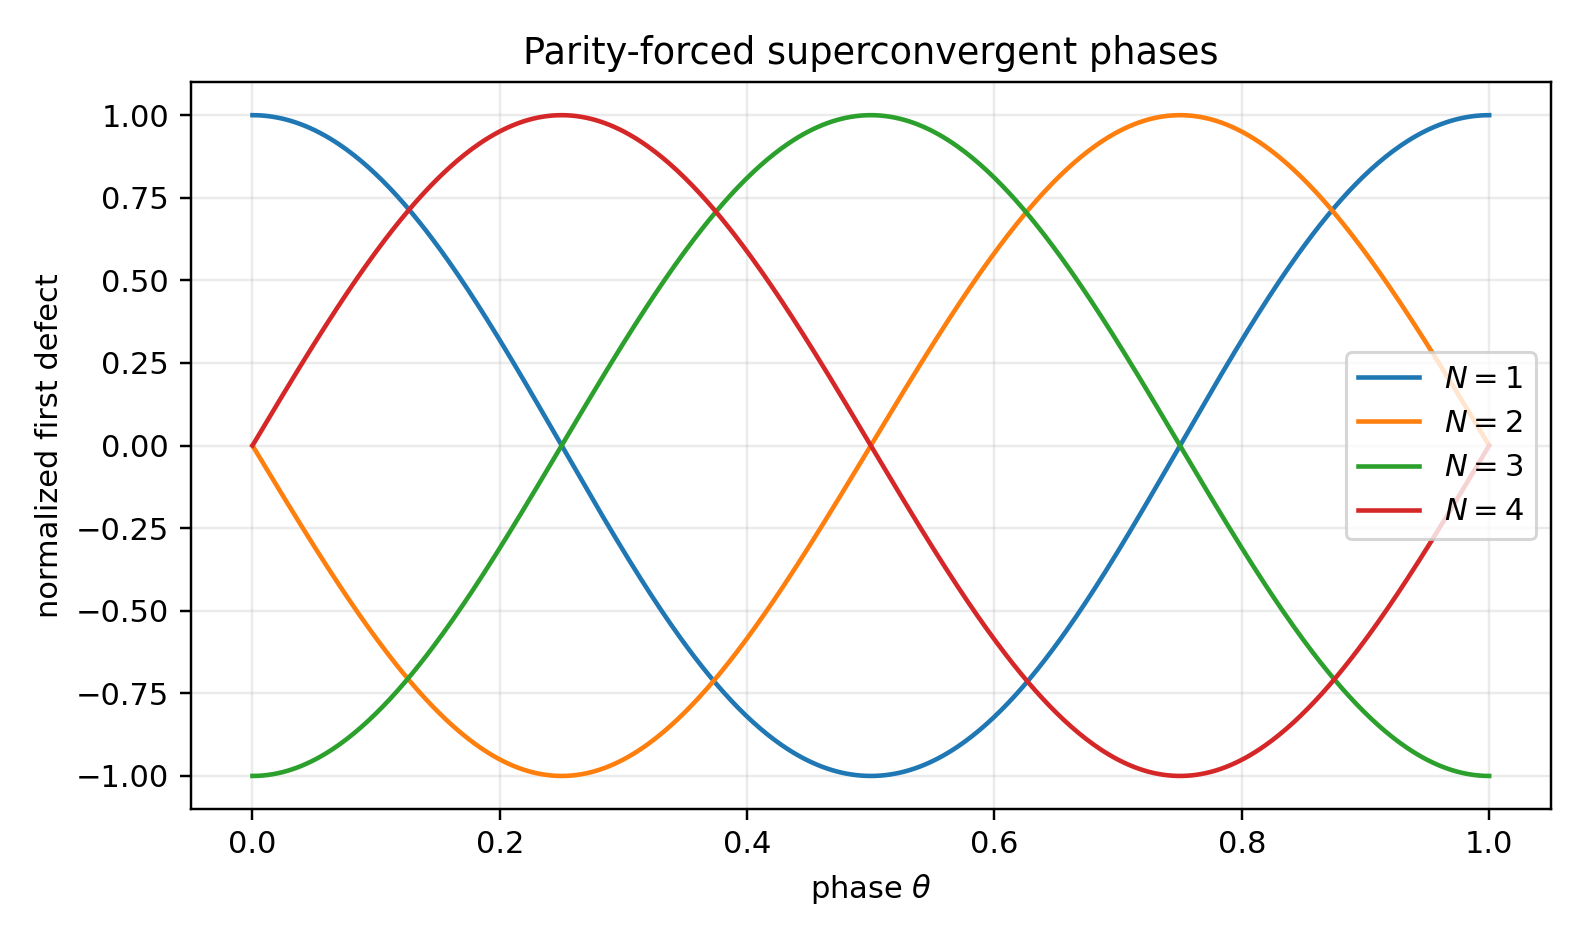
\includegraphics[width=0.88\textwidth]{assets/self-sampling/figures/defect_profiles.png}
\caption{Normalized exact first-defect profiles.  The parity-forced phases are common zeros of every odd harmonic in the corresponding sine or cosine series.}
\label{is:p3:fig:defect-profiles}
\end{figure}

\subsection{A canonical phase schedule and exact experiments}

Choose
\begin{equation}
 \theta_N=
 \begin{cases}
 0,&N\ \text{even},\\
 1/4,&N\ \text{odd}.
 \end{cases}
 \label{is:p3:eq:canonical-phase}
\end{equation}
Then $Q_{N,\theta_N}$ is positive, rational, and exact through degree $N+1$.  Its number of positive nodes is $2^{N+1}-1$ at centered levels and $2^{N+1}$ at quarter-shifted levels.

\begin{table}[H]
\centering
\caption{Exact rational checks of the canonical phase schedule.  ``Proved degree'' is the theorem above.  Each next defect is computed as an exact fraction; a decimal display is used here for legibility, while the full fractions are retained in the CSV and exact TeX table in the archive.}
\label{is:p3:tab:quadrature-exact}
% Generated by experiments.py; exact values are in the CSV
\begin{tabular}{@{}rrrrr@{}}
\toprule
$N$ & phase $\theta_N$ & positive nodes & proved degree & next defect (decimal display)\\
\midrule
0 & $0$ & 1 & 1 & $-0.11111111$\\
1 & $1/4$ & 4 & 2 & $0.011067708$\\
2 & $0$ & 7 & 3 & $0.0002806713$\\
3 & $1/4$ & 16 & 4 & $-2.189698e-6$\\
4 & $0$ & 31 & 5 & $-4.8411566e-9$\\
5 & $1/4$ & 64 & 6 & $3.0609753e-12$\\
6 & $0$ & 127 & 7 & $5.4077218e-16$\\
7 & $1/4$ & 256 & 8 & $-2.6505694e-20$\\
8 & $0$ & 511 & 9 & $-3.5647819e-25$\\
\bottomrule
\end{tabular}

\end{table}

\begin{figure}[H]
\centering
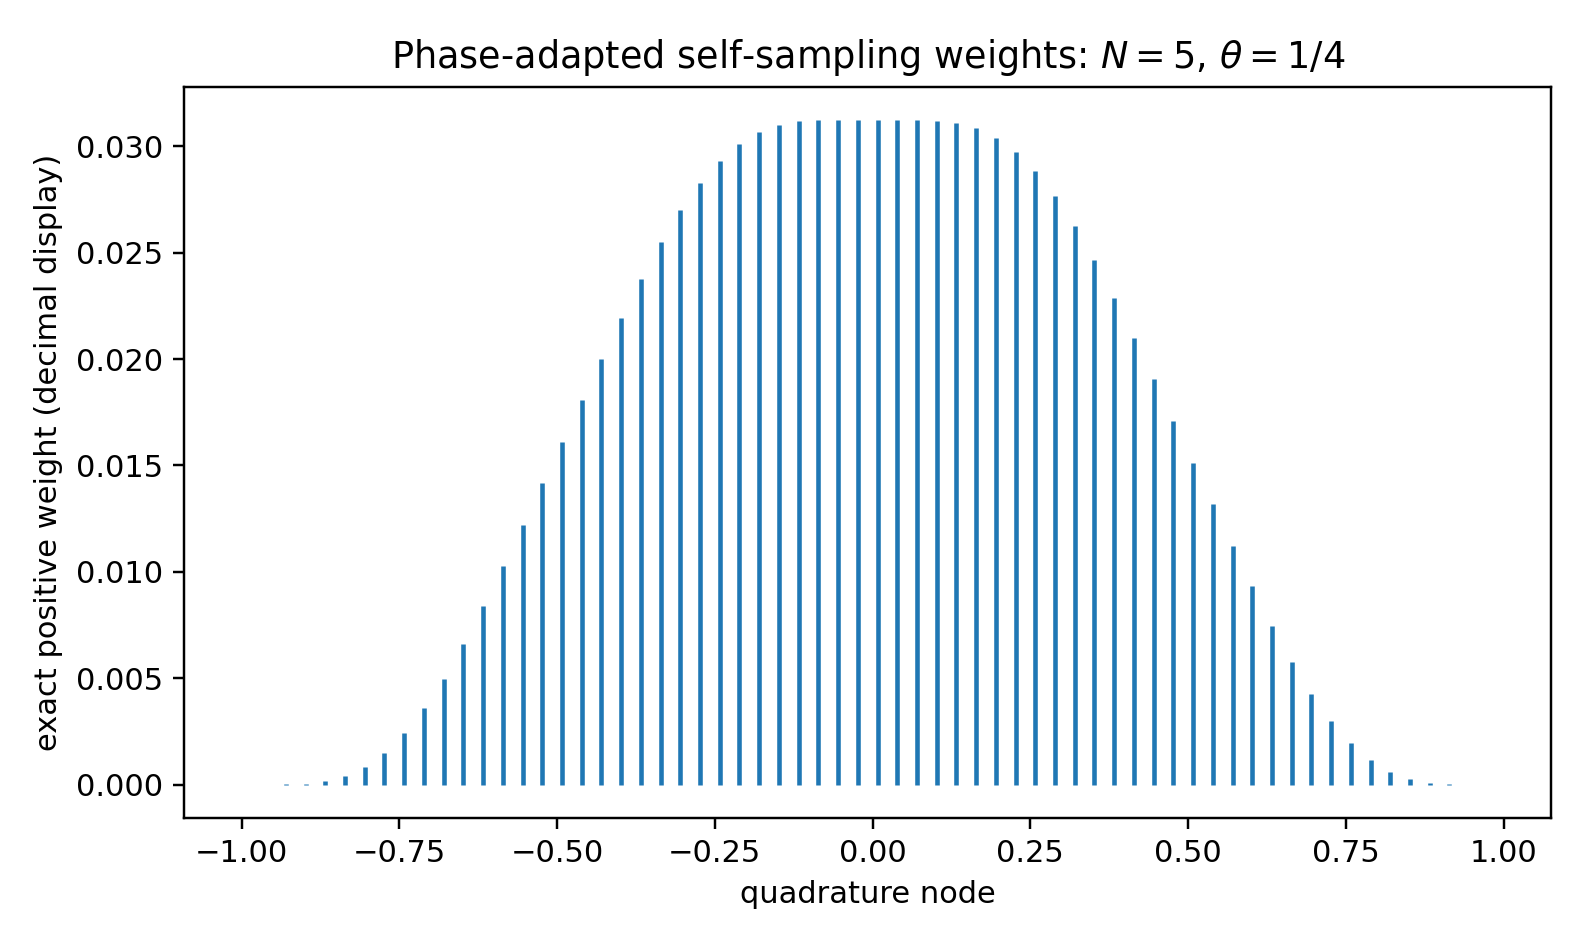
\includegraphics[width=0.88\textwidth]{assets/self-sampling/figures/quadrature_weights.png}
\caption{The positive rational weights at $N=5$, $\theta=1/4$.  The rule integrates every polynomial through degree six exactly.}
\label{is:p3:fig:quadrature-weights}
\end{figure}

The table proves by exact rational arithmetic that the canonical rule has
degree exactly $N+1$ for $0\le N\le8$.  The corresponding assertion for all
$N$, together with its experimentally observed sign refinement, is stated
once as \cref{is:p3:conj:next-defect-sign}; its exact two-layer formula is
derived in \cref{is:p3:app:next-defect}.

\section{Positive alias filters as Richardson extrapolation}
\label{is:p3:sec:positive-richardson}

\subsection{Coset rules}

For $s\ge0$ and $0\le a<2^s$, define the phase-coset rule
\begin{equation}
 Q_{N;s,a}[f]
 :=2^{-N}\sum_{k\in\IntegerNumbers}
 f\!\left(\frac{2^sk+a}{2^{N+s}}\right)
 u\!\left(\frac{2^sk+a}{2^{N+s}}\right).
 \label{is:p3:eq:coset-rule}
\end{equation}
This is simply $Q_{N,a/2^s}$, hence is positive and exact through degree $N$.

\begin{theorem}[Positive phase refinement]
\label{is:p3:thm:positive-phase-refinement}
For every $s\ge0$,
\begin{equation}
 \boxed{\displaystyle
 Q_{N+s,0}[f]
 =2^{-s}\sum_{a=0}^{2^s-1}Q_{N;s,a}[f].}
 \label{is:p3:eq:positive-phase-refinement}
\end{equation}
Thus averaging all $2^s$ positive phase classes gains exactly $s$ guaranteed degrees of polynomial exactness.
\end{theorem}

\begin{proof}
The integers $2^sk+a$, with $k\in\IntegerNumbers$ and $0\le a<2^s$, partition $\IntegerNumbers$.  Multiplying the outer factor $2^{-N}$ by $2^{-s}$ gives $2^{-(N+s)}$, exactly the fine-grid rule.
\end{proof}

For $s=1$, let
\[
 \nu_N=Q_{N,0},
 \qquad
 \rho_N=Q_{N,1/2}.
\]
Then
\begin{equation}
 \nu_{N+1}=\frac12(\nu_N+\rho_N),
 \qquad
 \boxed{\rho_N=2\nu_{N+1}-\nu_N.}
 \label{is:p3:eq:midpoint-Richardson}
\end{equation}
The right side is the familiar signed Richardson difference, yet the left side is manifestly a positive quadrature measure.  The cancellation that is hidden in scale space becomes positivity after resolution into even and odd lattice cosets.

\subsection{Uniqueness in alias space}

Suppose coefficients $c_0,\ldots,c_{2^s-1}$ combine the phase classes.  At Fourier alias $\ell$, the multiplier is
\begin{equation}
 C(\ell)=\sum_{a=0}^{2^s-1}c_a\EulerE^{2\pi\iu a\ell/2^s}.
 \label{is:p3:eq:DFT-filter}
\end{equation}
To gain all $s$ degrees, every residue class $\ell\not\equiv0\pmod{2^s}$ must be annihilated.

\begin{theorem}[Unique full residue-class filter]
\label{is:p3:thm:unique-phase-filter}
Assume
\begin{equation}
 C(0)=1,
 \qquad
 C(\ell)=0\quad(1\le\ell<2^s).
 \label{is:p3:eq:DFT-conditions}
\end{equation}
Then
\begin{equation}
 c_0=c_1=\cdots=c_{2^s-1}=2^{-s}.
 \label{is:p3:eq:unique-uniform-filter}
\end{equation}
Hence the positive average in \eqref{is:p3:eq:positive-phase-refinement} is the unique filter on all dyadic phases that cancels every nonzero residue class modulo $2^s$.
\end{theorem}

\begin{proof}
The vector $(C(0),\ldots,C(2^s-1))$ is the discrete Fourier transform of $(c_0,\ldots,c_{2^s-1})$.  Inverting the DFT of $(1,0,\ldots,0)$ gives the uniform vector.
\end{proof}

\begin{remark}[Comparison with $q$-Richardson]
The repository's geometric Lagrange/Richardson filters cancel powers of a scale parameter and generally use signed Gaussian-$q$-binomial weights.  The filter above cancels Fourier residue classes and uses equal positive weights.  The two mechanisms act in complementary variables: scale depth versus lattice phase.  Their tensor product is a natural candidate for a stable two-parameter accelerator; see \cref{is:p3:prob:hybrid-filter}.
\end{remark}

\begin{resultbox}[Third frontier bridge]
Subdividing a self-sampling rule does not merely refine a Riemann sum.  In Fourier space it applies an exact DFT projector to the alias tree.  The usual Richardson difference $2\nu_{N+1}-\nu_N$ is positive because it isolates the odd lattice coset.  This gives a rare instance in which an extrapolation operator has a hidden positive-measure realization.
\end{resultbox}

\section{Inverse-moment Rvachev--Appell polynomials}
\label{is:p3:sec:appell}

\subsection{The umbral inverse of the moment family}

The frontier volume already uses the forward moment Appell sequence
\begin{equation}
 \Pcal_n(x)=\int_{-1}^{1}(x+y)^n u(y)\Differential y,
 \qquad
 \sum_{n\ge0}\Pcal_n(x)\frac{z^n}{n!}=\EulerE^{xz}M(z).
 \label{is:p3:eq:forward-Appell}
\end{equation}
We now reverse the moment multiplier.

\begin{definition}[Sampling notation for the canonical Rvachev--Appell sequence]
\label{is:p3:def:inverse-Appell}
Set
\[
 \Acal_n(x):=A_n(x),
\]
where $A_n$ is the centered Rvachev--Appell sequence already defined in
\cref{is:p2:def:Appell-polys}.  Equivalently, its canonical generating
function reads
\begin{equation}
 \boxed{\displaystyle
 \frac{\EulerE^{xz}}{M(z)}
 =\sum_{n=0}^{\infty}\Acal_n(x)\frac{z^n}{n!}.}
 \label{is:p3:eq:inverse-Appell-gen}
\end{equation}
\end{definition}

Thus $\Acal_n$ is notation, not a second inverse-moment family.  Because
$M(0)=1$, the displayed series is well-defined formally and analytically near
$z=0$.  Its logarithm is
\begin{equation}
 xz-\sum_{r\ge1}\kappa_{2r}\frac{z^{2r}}{(2r)!}.
 \label{is:p3:eq:inverse-Appell-log}
\end{equation}

\begin{theorem}[Canonical Appell package in sampling notation]
\label{is:p3:thm:Appell-Bell}
Under the identification $\Acal_n=A_n$, the established Appell, Bell, and
operator identities take the following forms.
\begin{enumerate}
\item It is Appell and parity adapted:
\begin{equation}
 \Acal_n'(x)=n\Acal_{n-1}(x),
 \qquad
 \Acal_n(-x)=(-1)^n\Acal_n(x).
 \label{is:p3:eq:Appell-basic}
\end{equation}
\item It is a complete Bell polynomial in the Bernoulli cumulants:
\begin{equation}
 \boxed{\displaystyle
 \Acal_n(x)=Y_n(x,-\kappa_2,0,-\kappa_4,0,\ldots,-\kappa_n).}
 \label{is:p3:eq:Appell-Bell}
\end{equation}
\item It satisfies the triangular recurrence
\begin{equation}
 \Acal_{n+1}(x)
 =x\Acal_n(x)
 -\sum_{j=1}^{\Floor{(n+1)/2}}
 \binom n{2j-1}\kappa_{2j}\Acal_{n-2j+1}(x).
 \label{is:p3:eq:Appell-recurrence}
\end{equation}
\item The forward and inverse families are umbral inverses:
\begin{equation}
 M(D)\Acal_n(x)=x^n,
 \qquad
 M(D)^{-1}\Pcal_n(x)=x^n,
 \qquad D=\frac{\Differential}{\Differential x}.
 \label{is:p3:eq:umbral-inverse}
\end{equation}
\end{enumerate}
\end{theorem}

\begin{proof}
The Appell law is \eqref{is:p2:eq:Appell-derivative}, and parity follows at
once from the evenness of $M$ in the canonical generating function
\eqref{is:p2:eq:A-generating}.  Combining the canonical Bell reconstruction
\eqref{is:p2:eq:alpha-Bell} with the translation formula
\eqref{is:p2:eq:A-from-alpha} gives \eqref{is:p3:eq:Appell-Bell}; equivalently,
it is the defining complete-Bell expansion of
\eqref{is:p3:eq:inverse-Appell-log}.  The only additional displayed formula is
the convenient triangular form.  Differentiating the generating function
with respect to $z$ gives
\[
 \frac{\partial}{\partial z}\frac{\EulerE^{xz}}{M(z)}
 =\left(x-\frac{M'(z)}{M(z)}\right)\frac{\EulerE^{xz}}{M(z)},
\]
and coefficient comparison gives \eqref{is:p3:eq:Appell-recurrence}.  Finally,
the first identity in \eqref{is:p3:eq:umbral-inverse} is the canonical operator
formula \eqref{is:p2:eq:A-operator}.  The generating function
\eqref{is:p3:eq:forward-Appell} says $\Pcal_n=M(D)x^n$; applying
$M(D)^{-1}$ proves the second identity.
\end{proof}

The first polynomials are reproduced in \cref{is:p3:app:Appell-table}.  In compact notation,
\begin{align*}
 \Acal_2(x)&=x^2-\frac19,\\
 \Acal_4(x)&=x^4-\frac23x^2+\frac{31}{675},\\
 \Acal_6(x)&=x^6-\frac53x^4+\frac{31}{45}x^2-\frac{2347}{59535}.
\end{align*}
The constants are the signed complete Bell transforms of the rational cumulants; no transcendental constants remain.

\subsection{Continuous deconvolution}

\begin{theorem}[Exact deconvolution identity]
\label{is:p3:thm:Appell-deconvolution}
For every $n\ge0$ and $x\in\RealNumbers$,
\begin{equation}
 \boxed{\displaystyle
 \int_{-1}^{1}\Acal_n(x-y)u(y)\Differential y=x^n.}
 \label{is:p3:eq:Appell-deconvolution}
\end{equation}
Equivalently, the convolution operator by $u$ maps the inverse-moment Appell basis to the monomial basis.
\end{theorem}

\begin{proof}
This is the centered mean-value inversion
\eqref{is:p2:eq:mean-value-inversion}, with symmetry replacing $Y$ by $-Y$.
For completeness, the generating-function proof that will be discretized
below is as follows.  Multiply generating functions:
\begin{align*}
 \int_{-1}^{1}\frac{\EulerE^{(x-y)z}}{M(z)}u(y)\Differential y
 &=\frac{\EulerE^{xz}}{M(z)}M(-z)\\
 &=\EulerE^{xz},
\end{align*}
using the evenness $M(-z)=M(z)$.  Compare coefficients of $z^n/n!$.
\end{proof}

\begin{corollary}[Mean-zero Appell cancellations]
\label{is:p3:cor:Appell-mean-zero}
For $n\ge1$,
\begin{equation}
 \int_{-1}^{1}\Acal_n(x)u(x)\Differential x=0.
 \label{is:p3:eq:Appell-mean-zero}
\end{equation}
\end{corollary}

\begin{proof}
Set $x=0$ in \eqref{is:p3:eq:Appell-deconvolution} and use parity.
\end{proof}

\subsection{Finite lattice reproduction}

The self-sampling theorem discretizes the deconvolution identity without loss.

\begin{theorem}[Finite Rvachev--Appell translation formula]
\label{is:p3:thm:Appell-lattice-reproduction}
Let $N\ge0$, $\theta\in\RealNumbers$, and $0\le n\le N$.  Then, for every $x\in\RealNumbers$,
\begin{equation}
 \boxed{\displaystyle
 x^n=2^{-N}\sum_{k\in\IntegerNumbers}
 \Acal_n\!\left(x-\frac{k+\theta}{2^N}\right)
 u\!\left(\frac{k+\theta}{2^N}\right).}
 \label{is:p3:eq:Appell-lattice-reproduction}
\end{equation}
The sum is finite.  At a superconvergent phase from \cref{is:p3:cor:forced-superconvergence}, the identity remains valid for $n=N+1$.
\end{theorem}

\begin{proof}
For fixed $x$, the map $y\mapsto\Acal_n(x-y)$ is a polynomial of degree $n$.  Apply \cref{is:p3:thm:self-sampling} to the integral in \eqref{is:p3:eq:Appell-deconvolution}.
\end{proof}

More generally, for a polynomial $p$ define its Rvachev deconvolution
\begin{equation}
 \mathscr D_{\RvachevUp}p
 :=M(D)^{-1}p
 =\exp\!\left(-\sum_{r\ge1}\kappa_{2r}
 \frac{D^{2r}}{(2r)!}\right)p.
 \label{is:p3:eq:polynomial-deconvolution}
\end{equation}
The exponential truncates because $p$ is a polynomial.

\begin{corollary}[Polynomial reproduction by deconvolved translates]
\label{is:p3:cor:polynomial-deconvolution}
If $\deg p\le N$, then
\begin{equation}
 p(x)=2^{-N}\sum_{k\in\IntegerNumbers}
 (\mathscr D_{\RvachevUp}p)\!\left(x-\frac{k+\theta}{2^N}\right)
 u\!\left(\frac{k+\theta}{2^N}\right).
 \label{is:p3:eq:general-deconvolution-reproduction}
\end{equation}
\end{corollary}

\begin{proof}
Write $p(x)=\sum_{n=0}^{N}c_nx^n$.  The defining generating function gives
$M(D)^{-1}x^n=\Acal_n(x)$, hence
$\mathscr D_{\RvachevUp}p=\sum_{n=0}^{N}c_n\Acal_n$.  Apply
\Cref{is:p3:thm:Appell-lattice-reproduction} to each monomial and sum with
coefficients $c_n$.  Every sum is finite because $u$ is compactly supported,
so the interchange is purely finite and yields
\eqref{is:p3:eq:general-deconvolution-reproduction}.
\end{proof}

\begin{statusbox}[Lean status of Appell deconvolution and lattice reproduction]
Three source rows in this section now have exact compiled counterparts.
The centered identity \cref{is:p3:thm:Appell-deconvolution} is
\path{Fabius.integral_eval_rvachevAppellPolynomial_sub_mul_rvachev}; its
general polynomial companion is
\path{Fabius.integral_eval_rvachevDeconvolvedPolynomial_sub_mul_rvachev}.
The mean-zero corollary \cref{is:p3:cor:Appell-mean-zero} is
\path{Fabius.integral_eval_rvachevAppellPolynomial_mul_rvachev_eq_zero}, and
\cref{is:p3:cor:polynomial-deconvolution} is
\path{Fabius.normalized_tsum_shifted_rvachevDeconvolvedPolynomial_mul_rvachevUp}.
Compact support reduces the first two whole-line integrals to the displayed
interval \([-1,1]\).  The last declaration has the same nonzero natural mesh,
degree bound, arbitrary real phase, normalized physical-coordinate nodes, and
conclusion as the paper.

The full finite-lattice theorem is now formalized by an explicit two-part
family.  For arbitrary phase and $0\le n\le N$, specialize
\path{Fabius.normalized_tsum_shifted_rvachevDeconvolvedPolynomial_mul_rvachevUp}
to $M=2^N$ and $P=X^n$.  At a selected phase, including the endpoint and
midpoint pair for even $N$ and the quarter pair for odd $N$,
\path{Fabius.normalized_tsum_shifted_rvachevAppellPolynomial_mul_rvachevUp_superconvergent}
proves the same formula through $n=N+1$; the exact phase dictionary is
\path{Fabius.isRvachevSuperconvergentPhase_two_pow_iff}.  Finally,
\path{Fabius.finite_support_comb} supplies the asserted finiteness.  Thus
\cref{is:p3:thm:Appell-lattice-reproduction} is Lean-proved.  No uniqueness
or sharpness assertion about the selected phases is included in this status.
\end{statusbox}

\begin{resultbox}[Fourth frontier bridge]
The forward moment Appell family packages convolution by the up-law; the reciprocal family $\Acal_n$ packages deconvolution.  The same positive dyadic samples that integrate ordinary polynomials now reproduce ordinary monomials from translates of $\Acal_n$.  This simultaneously connects the Fourier zeros, Bernoulli cumulants, complete Bell polynomials, and finite rational Fabius values.
\end{resultbox}

\subsection{Root geometry: an exact counterexample to real-rootedness}

Numerically, the first seven polynomials have only real zeros.  Degree eight
already supplies an exact counterexample to global real-rootedness; without
exact certificates in degrees one through seven, we do not claim that it is
the first such degree.

\begin{proposition}[Exact degree-eight nonreal-zero certificate]
\label{is:p3:prop:A8-roots}
The exact polynomial
\begin{equation}
 \Acal_8(x)
 =x^8-\frac{28}{9}x^6+\frac{434}{135}x^4
 -\frac{9388}{8505}x^2+\frac{1904369}{32531625}
 \label{is:p3:eq:A8}
\end{equation}
has exactly four real zeros.  Hence its other four zeros are nonreal and form two conjugate pairs.
\end{proposition}

\begin{proof}[Computer-assisted exact proof]
Let $S_0=\Acal_8$, $S_1=S_0'$, and
$S_{j+1}=-\operatorname{rem}(S_{j-1},S_j)$ in $\RationalNumbers[x]$.
Exact Euclidean division produces nine nonzero terms, ending in the positive
constant $1904369/32531625$.  After clearing only positive rational factors,
their degrees and limiting signs are
\[
\begin{array}{c|rrrrrrrrr|c}
j&0&1&2&3&4&5&6&7&8&V\\ \hline
\deg S_j&8&7&6&5&4&3&2&1&0&\\
\Sign S_j(-\infty)&+&-&+&-&+&+&+&-&+&6\\
\Sign S_j(+\infty)&+&+&+&+&+&-&+&+&+&2
\end{array}
\]
The complete primitive integer sequence and its positive scale factors are
recorded in
\path{assets/self-sampling/appell_a8_sturm_certificate.txt}; each row may be
checked by one exact polynomial division.  Sturm's theorem therefore gives
$V(-\infty)-V(+\infty)=6-2=4$ distinct real roots.  Because the sequence
ends in a nonzero constant, $S_0$ is square-free.  Its remaining four roots
are nonreal; real coefficients pair them into two conjugate pairs.  No
floating-point root classification enters the proof.
\end{proof}

\begin{figure}[H]
\centering
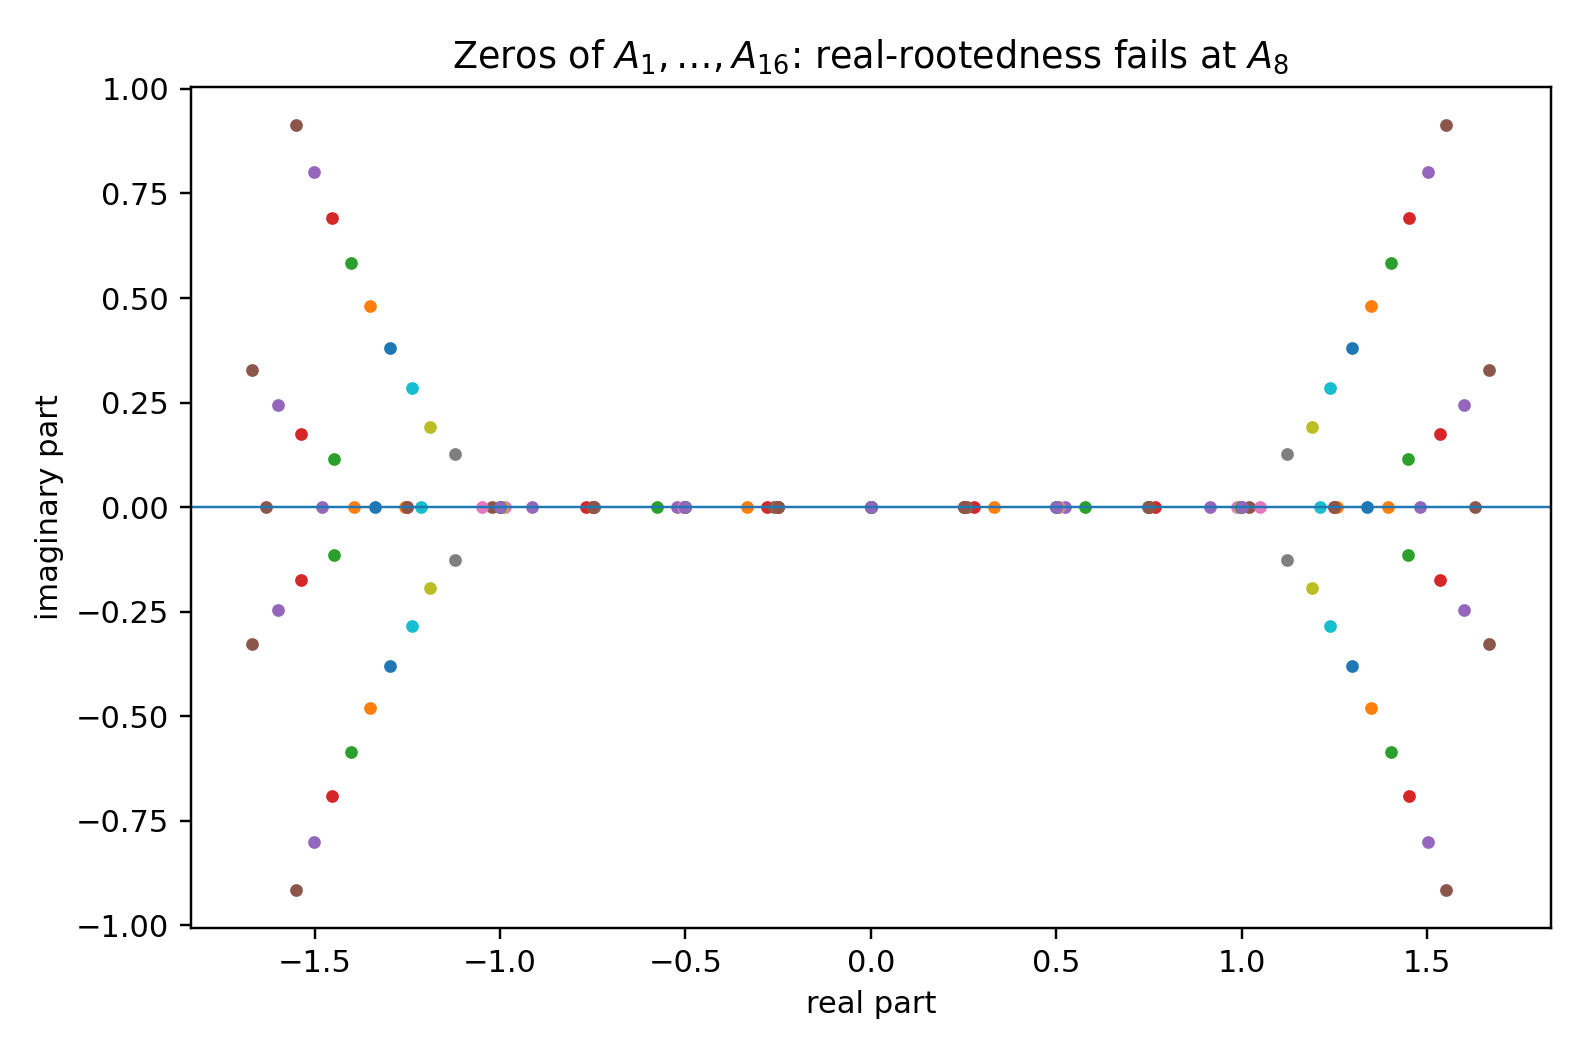
\includegraphics[width=0.86\textwidth]{assets/self-sampling/figures/appell_roots.png}
\caption{Numerical locations of the zeros of $\Acal_1,\ldots,\Acal_{16}$.
The Sturm calculation certifies the degree-eight departure from the real
axis; the apparent absence of earlier departures and the later pattern are
exploratory.}
\label{is:p3:fig:Appell-roots}
\end{figure}

The computed nonreal-root counts through degree $30$ are
\begin{center}
\begin{tabular}{@{}lrrrrrr@{}}
\toprule
Degree range & $1$--$7$ & $8$--$12$ & $13$--$17$ & $18$--$22$ & $23$--$28$ & $29$--$30$\\
\midrule
Nonreal roots & $0$ & $4$ & $8$ & $12$ & $16$ & $20$\\
\bottomrule
\end{tabular}
\end{center}
This staircase is not asserted as a theorem; it motivates \cref{is:p3:conj:Appell-root-staircase}.

\section{Transport through the inverse Fabius function}
\label{is:p3:sec:inverse-transport}

The centered quantile $q(t)=2F^{-1}(t)-1$ pushes Lebesgue measure on $[0,1]$ to the up-law.  Therefore
\begin{equation}
 \int_0^1g(q(t))\Differential t=\int_{-1}^{1}g(x)u(x)\Differential x
 \label{is:p3:eq:quantile-transport}
\end{equation}
for every bounded Borel function $g$.

\begin{theorem}[Rational inverse-Fabius quadrature]
\label{is:p3:thm:inverse-Fabius-quadrature}
Let $\theta=a/2^s$ and retain the dyadic nodes $x_k=n_k/2^D$ and weights $w_k$ from \cref{is:p3:cor:rational-rules}.  Define
\begin{equation}
 t_k=F\!\left(\frac{1+x_k}{2}\right)\in\RationalNumbers.
 \label{is:p3:eq:inverse-Fabius-nodes}
\end{equation}
Then $q(t_k)=x_k$, and for every polynomial $p$ with $\deg p\le N$,
\begin{equation}
 \boxed{\displaystyle
 \int_0^1p\bigl(2F^{-1}(t)-1\bigr)\Differential t
 =\sum_k w_k\,p\bigl(2F^{-1}(t_k)-1\bigr)
 =\sum_k w_kp(x_k).}
 \label{is:p3:eq:inverse-Fabius-quadrature}
\end{equation}
At a phase-superconvergent level the exactness extends to $\deg p\le N+1$.
\end{theorem}

\begin{proof}
Equation \eqref{is:p3:eq:centered-CDF} implies $q(t_k)=x_k$.  Apply \eqref{is:p3:eq:quantile-transport} and then \cref{is:p3:thm:self-sampling}.  Rationality follows because both $(1+x_k)/2$ and the weight arguments are dyadic.
\end{proof}

\begin{remark}[A nonlinear exactness space]
The rule in \eqref{is:p3:eq:inverse-Fabius-quadrature} is not claimed to integrate all ordinary polynomials in $t$.  It integrates exactly the non-elementary space
\begin{equation}
 \mathcal V_N
 =\SpanOperator\{1,q(t),q(t)^2,\ldots,q(t)^N\},
 \qquad q(t)=2F^{-1}(t)-1,
 \label{is:p3:eq:inverse-exactness-space}
\end{equation}
using rational nodes $t_k$, rational weights $w_k$, and no numerical inversion.  This is an exact finite interface between the inverse Fabius function and dyadic arithmetic.
\end{remark}

\subsection{Endpoint nodes and the Lambert coordinate}

For centered rules, the smallest nonzero endpoint distance is $2^{-N}$ and the corresponding extreme weights are
\begin{equation}
 2^{-N}F(2^{-N}).
 \label{is:p3:eq:centered-extreme-weight}
\end{equation}
For quarter-shifted rules, the leftmost distance is $2^{-N-2}$, so one extreme weight is
\begin{equation}
 2^{-N}F(2^{-N-2}).
 \label{is:p3:eq:quarter-extreme-weight}
\end{equation}
The corpus's sharp endpoint theory expresses $F(x)$ through the exact lower-Lambert coordinate
\begin{equation}
 \lambda(x)=-\frac1{\log2}W_{-1}(-x\log2),
 \qquad x=\lambda2^{-\lambda},
 \label{is:p3:eq:Lambert-coordinate}
\end{equation}
with a nonconstant periodic correction in the dyadic phase of $\lambda$.  Thus the new quadrature rules supply exact rational global moment constraints whose smallest weights lie precisely in the Lambert boundary layer.  Turning these constraints into identities for the endpoint periodic factor is an open program formulated in \cref{is:p3:prob:Lambert-sum-rules}.

\section{Finite Gaussian-\texorpdfstring{$q$}{q}-binomial identities forced by quadrature}
\label{is:p3:sec:qbinomial}

\subsection{The exact dyadic evaluator}

Let
\begin{equation}
 (q;q)_n=\prod_{j=1}^{n}(1-q^j),
 \qquad
 \GaussianBinomial{n}{k}{q}=\frac{(q;q)_n}{(q;q)_k(q;q)_{n-k}}.
 \label{is:p3:eq:q-notation-report}
\end{equation}
For integers $m,n\ge0$ and $c\in\RationalNumbers$, define
\begin{equation}
\begin{aligned}
 \mathfrak Q_n(m;c)
 :={}&\frac{1}{2^{n^2}(1/2;1/2)_n}
 \sum_{j=0}^{n}
 \frac{\GaussianBinomial{n}{j}{1/2}}
      {2^{j(j-1)}(n+j)!}\\
 &\qquad\times
 \sum_{r=0}^{m2^j-1}\eps_r
 \bigl(r-m2^j+c\bigr)^{n+j}.
 \label{is:p3:eq:Qfrak-def}
\end{aligned}
\end{equation}
The established arbitrary-numerator theorem states
\begin{equation}
 \mathfrak Q_n(m;c)=F(m/2^n)
 \qquad(0\le m\le2^n),
 \label{is:p3:eq:Qfrak-F}
\end{equation}
and the right side of \eqref{is:p3:eq:Qfrak-def} is independent of $c$.  Its Gaussian coefficients arise from Lagrange interpolation on a geometric grid.

\subsection{A \texorpdfstring{$q$}{q}-binomial--Thue--Morse--Bell identity}

\begin{theorem}[Finite arithmetic moment identity]
\label{is:p3:thm:qbinomial-moment-identity}
Let $\theta=a/2^s$, $D=N+s$, $n_k=2^sk+a$, and $b_k=2^D-\AbsoluteValue{n_k}$.  For every $0\le r\le N$ and every $c\in\RationalNumbers$,
\begin{equation}
 \boxed{\displaystyle
 \mu_r
 =2^{-N-Dr}
 \sum_{\AbsoluteValue{n_k}<2^D}
 n_k^r\,\mathfrak Q_D(b_k;c).}
 \label{is:p3:eq:qbinomial-moment-identity}
\end{equation}
At the superconvergent phases of \cref{is:p3:cor:forced-superconvergence}, the identity also holds for $r=N+1$.  Therefore the finite Gaussian-$q$-binomial--Thue--Morse sum on the right equals
\begin{equation}
 Y_r(0,\kappa_2,0,\kappa_4,\ldots,\kappa_r),
 \label{is:p3:eq:qbinomial-Bell-right}
\end{equation}
where the cumulants are the Bernoulli rationals in \eqref{is:p3:eq:cumulants}.
\end{theorem}

\begin{proof}
At node $x_k=n_k/2^D$, \eqref{is:p3:eq:F-up-relation} and \eqref{is:p3:eq:Qfrak-F} give
\[
 u(x_k)=F(b_k/2^D)=\mathfrak Q_D(b_k;c).
\]
Substitute this into \eqref{is:p3:eq:self-sampling-main}, then use \eqref{is:p3:eq:moment-Bell}.
\end{proof}

\begin{remark}[Why this identity is structurally new]
Each ingredient existed separately: the $q$-binomial evaluator, the Bell moment formula, and the zero multiplicities.  The self-sampling theorem forces them into a single positive finite identity.  The common translation $c$ disappears after a double finite summation, giving a family of nontrivial translation-invariance identities among Thue--Morse power sums.
\end{remark}

\begin{corollary}[Finite Appell cancellation in $q$-arithmetic]
\label{is:p3:cor:q-Appell-cancellation}
For $1\le n\le N$,
\begin{equation}
 \sum_{\AbsoluteValue{n_k}<2^D}
 \Acal_n\!\left(-\frac{n_k}{2^D}\right)
 \mathfrak Q_D(b_k;c)=0.
 \label{is:p3:eq:q-Appell-cancellation}
\end{equation}
After inserting \eqref{is:p3:eq:Qfrak-def}, this is a finite identity containing Gaussian $q$-binomial coefficients, Thue--Morse signs, Bernoulli cumulants, and complete Bell polynomials.
\end{corollary}

\begin{proof}
Set $x=0$ in \eqref{is:p3:eq:Appell-lattice-reproduction} and clear the common factor $2^{-N}$.
\end{proof}

\section{Base-\texorpdfstring{$b$}{b} and multidimensional extensions}
\label{is:p3:sec:extensions}

\subsection{Integer dilation bases}

Let $b\ge2$ be an integer and define
\begin{equation}
 \Phi_b(\xi)=\prod_{j=0}^{\infty}
 \SincPi\!\left(\frac{\xi}{b^j}\right).
 \label{is:p3:eq:Phi-b}
\end{equation}

\begin{proposition}[Construction and regularity of the base-$b$ density]
\label{is:p3:prop:base-b-density}
Let $(U_j)_{j\ge0}$ be independent, with $U_j$ uniform on
\[
 I_j=\left[-\frac1{2b^j},\frac1{2b^j}\right].
\]
Then the series $S_b=\sum_{j\ge0}U_j$ converges absolutely.  Its law has a
nonnegative density $u_b\in C_c^\infty(\RealNumbers)$ satisfying
\begin{equation}
 \FourierTwoPi{u_b}(\xi)=\Phi_b(\xi),
 \qquad
 \int_{\RealNumbers}u_b(x)\Differential x=1,
 \qquad
 \SupportOperator(u_b)=
 \left[-\frac{b}{2(b-1)},\frac{b}{2(b-1)}\right].
 \label{is:p3:eq:base-b-density-properties}
\end{equation}
Thus $u_b$ is precisely the infinite convolution of the centered uniform
density factors.
\end{proposition}

\begin{proof}
The deterministic estimate
\[
 \sum_{j\ge0}\AbsoluteValue{U_j}
 \le\frac12\sum_{j\ge0}b^{-j}=\frac{b}{2(b-1)}
\]
proves absolute convergence.  The $j$th uniform law has Fourier transform
$\SincPi(\xi/b^j)$, so independence and convergence of the partial sums give
$\Expectation\EulerE^{-2\pi\iu\xi S_b}=\Phi_b(\xi)$.

It remains to justify that this probability law is smooth rather than merely
a compactly supported measure.  The elementary estimate
\[
 \AbsoluteValue{\SincPi t}\le
 \min\left(1,\frac1{\pi\AbsoluteValue t}\right)
\]
shows, by retaining any fixed number $K$ of factors in
\eqref{is:p3:eq:Phi-b}, that
\[
 \AbsoluteValue{\Phi_b(\xi)}\le C_K(1+\AbsoluteValue\xi)^{-K}
 \qquad(\xi\in\RealNumbers)
\]
for some constant $C_K$.  Hence $\xi^r\Phi_b(\xi)$ is integrable for every
$r\ge0$.  Fourier inversion therefore supplies a $C^r$ density for every
$r$, and differentiating under the inverse-transform integral identifies all
of its derivatives.  Thus $u_b\in C^\infty$.  Since it represents a
probability law, it is nonnegative and has integral one.

For the exact support, equip $\prod_{j\ge0}I_j$ with the product measure.  It
has full support, and the summation map is continuous because the defining
series converges uniformly.  Its image is the interval
\[
 \sum_{j\ge0}I_j=
 \left[-\frac12\sum_{j\ge0}b^{-j},
        \frac12\sum_{j\ge0}b^{-j}\right]
 =\left[-\frac{b}{2(b-1)},\frac{b}{2(b-1)}\right].
\]
(For example, every point in this interval is obtained by choosing all
coordinates in the same fixed proportion of their respective endpoints.)
The continuous image of this full-support product measure consequently has
exactly that interval as its support.  This proves
\eqref{is:p3:eq:base-b-density-properties}.
\end{proof}

If $m\ne0$ is an integer, then
\begin{equation}
 \OrderOperator_{\xi=m}\Phi_b=1+\nu_b(m),
 \label{is:p3:eq:b-multiplicity}
\end{equation}
where $\nu_b(m)$ is the largest $a$ such that $b^a\mid m$.
Indeed, precisely the factors with $0\le j\le\nu_b(m)$ vanish at $m$; each
has a simple zero there, and every later factor is nonzero.

\begin{theorem}[Base-$b$ self-sampling]
\label{is:p3:thm:base-b}
For every $N\ge0$, phase $\theta$, and polynomial $p$ of degree at most $N$,
\begin{equation}
 \int p(x)u_b(x)\Differential x
 =b^{-N}\sum_{k\in\IntegerNumbers}
 p\!\left(\frac{k+\theta}{b^N}\right)
 u_b\!\left(\frac{k+\theta}{b^N}\right).
 \label{is:p3:eq:base-b-self-sampling}
\end{equation}
Moreover, averaging the $b^s$ phases $a/b^s$ gives the level-$N+s$ rule and is
the unique normalized full DFT filter: among coefficient vectors $(c_a)$ with
$\sum_a c_a=1$, it is the only one annihilating every nonzero residue modulo
$b^s$.
\end{theorem}

\begin{proof}
By \cref{is:p3:prop:base-b-density}, the functions
$x^ru_b(x)$ are smooth and compactly supported, so Poisson summation applies.
For $0\le r\le N$, its nonzero alias at $b^N\ell$ is a constant multiple of
$\Phi_b^{(r)}(b^N\ell)$.  Equation \eqref{is:p3:eq:b-multiplicity} gives
\[
 \OrderOperator_{\xi=b^N\ell}\Phi_b
 =N+1+\nu_b(\ell)>r,
\]
so every such alias vanishes.  The zero alias is the $r$th moment.  This proves
\eqref{is:p3:eq:base-b-self-sampling} for monomials and hence for all stated
polynomials.

For the phase refinement, average the rules with phases $a/b^s$.  Writing
$r=b^sk+a$ identifies their nodes bijectively with $r/b^{N+s}$, and the
averaged coefficient is $b^{-(N+s)}$; the result is exactly the level-$N+s$
rule.  Finally, normalized weights $c_a$ with $\sum_a c_a=1$ annihilate every
nonzero residue precisely when their $b^s$-point discrete Fourier transform is
$(1,0,\ldots,0)$.  Fourier
inversion gives $c_a=b^{-s}$ for every $a$, proving uniqueness.
\end{proof}

The binary case is distinguished arithmetically because half-integer spectral signs reduce to the classical Thue--Morse sequence and dyadic Fabius values are rational.  For general $b$, the same analytic framework suggests generalized digital sign sequences and $q=b^{-1}$ arithmetic.

\subsection{Tensor-product cubature}

Let
\begin{equation}
 U_d(x_1,\ldots,x_d)=\prod_{j=1}^{d}u(x_j).
 \label{is:p3:eq:tensor-density}
\end{equation}
Tensoring \cref{is:p3:thm:self-sampling} gives a positive cubature rule.

\begin{corollary}[Positive tensor cubature]
\label{is:p3:cor:tensor-cubature}
For a polynomial $p$ whose degree in each coordinate is at most $N$,
\begin{equation}
 \int_{[-1,1]^d}p(\bm x)U_d(\bm x)\Differential\bm x
 =2^{-Nd}\sum_{\bm k\in\IntegerNumbers^d}
 p\!\left(\frac{\bm k+\bm\theta}{2^N}\right)
 U_d\!\left(\frac{\bm k+\bm\theta}{2^N}\right).
 \label{is:p3:eq:tensor-cubature}
\end{equation}
The sum is finite and positive.  Coordinatewise phase superconvergence raises the exactness by one in every selected coordinate.
\end{corollary}

\begin{proof}
It is enough by linearity to take
$p(\bm x)=\prod_{j=1}^{d}x_j^{r_j}$ with $0\le r_j\le N$.  Fubini's theorem
factors the integral into $d$ one-dimensional moments.  Apply
\Cref{is:p3:thm:self-sampling} to each factor and multiply the resulting
finite sums; their Cartesian product is exactly
\eqref{is:p3:eq:tensor-cubature}.  Compact support makes the sum finite, and
every weight is nonnegative because $u\ge0$.  If a chosen coordinate phase
satisfies the cancellation condition of
\Cref{is:p3:cor:forced-superconvergence}, the same argument admits
$r_j=N+1$ in that coordinate; applying this independently proves the final
coordinatewise assertion.
\end{proof}

The node count grows exponentially with $d$, so sparse-grid combinations and hyperbolic-cross alias filters are a natural next step; see \cref{is:p3:prob:sparse-grid}.

% Source fragment: Inverse and sampling frontiers; prefix is.
\section{Conjectures and frontier research program}
\label{is:p3:sec:frontier}

\subsection{The next alias layer}

\begin{conjecture}[Exact phase-adapted precision and sign]
\label{is:p3:conj:next-defect-sign}
Let $\theta_N$ be the canonical phase in \eqref{is:p3:eq:canonical-phase}.  Then
\begin{equation}
 E_{N,N+2}(\theta_N)\ne0
 \qquad(N\ge0).
 \label{is:p3:eq:next-defect-nonzero}
\end{equation}
Moreover, for $N\ge1$, the experimental sign law is
\begin{equation}
 \Sign E_{N,N+2}(\theta_N)
 =(-1)^{\Floor{(N-1)/2}}.
 \label{is:p3:eq:next-defect-sign-conj}
\end{equation}
\end{conjecture}

The exact two-layer formula is given in \cref{is:p3:app:next-defect}.  A proof should combine:
\begin{enumerate}
\item the odd-alias contribution with one Bell correction $\gamma_1$;
\item the twice-odd contribution with its leading zero jet;
\item the parity-specific phase factors;
\item a first-frequency dominance estimate sharp enough to control the logarithmic derivative $\PhiCyc'/\PhiCyc$ at half-integers.
\end{enumerate}
A successful argument would determine the exact degree of every positive phase-adapted rule.

\begin{problem}[All higher phase gains]
\label{is:p3:prob:higher-phase-gains}
For fixed excess $s\ge2$, classify all phases $\theta$ for which
\[
 E_{N,N+1}(\theta)=\cdots=E_{N,N+s}(\theta)=0.
\]
The valuation filtration makes this a finite hierarchy of trigonometric equations built from alias layers $0,\ldots,s-1$.  Determine whether any single positive phase can gain more than one degree for infinitely many $N$.
\end{problem}

\subsection{Optimal phase and scale filters}

\begin{problem}[Hybrid DFT--Gaussian-$q$ filter]
\label{is:p3:prob:hybrid-filter}
Combine the positive DFT projector in \eqref{is:p3:eq:positive-phase-refinement} with the repository's geometric Gaussian-$q$-binomial Richardson filters in the scale variable.  For a prescribed exactness order, minimize:
\begin{enumerate}
\item total variation of the combined coefficients;
\item number of distinct dyadic Fabius evaluations;
\item largest denominator of an exact rational coefficient;
\item sensitivity near the flat endpoints.
\end{enumerate}
A two-stage construction may first remove low $2$-adic alias classes by positive phase averaging and then remove the remaining scale modes by a short signed $q$-Richardson filter.
\end{problem}

\begin{problem}[Sparse positive phase design]
\label{is:p3:prob:sparse-positive-phase}
Fix $s\ge2$ and $1\le q<2^s$.  Among probability vectors
$c=(c_0,\ldots,c_{2^s-1})$ with at most $q$ nonzero entries, determine
\[
 \min_c\;\max_{1\le r<2^s}
 \left|\sum_{a=0}^{2^s-1}c_a
       \EulerE^{2\pi\ImaginaryUnit ar/2^s}\right|,
\]
classify the minimizers up to cyclic symmetry, and, among tied minimizers,
minimize $\sum_ac_a^2$.  Determine how the optimal leakage controls the
worst first surviving alias of the associated positive sampling rule.
\end{problem}

The former ``positive extremality'' conjecture imposed all exact DFT
annihilation equations.  By \Cref{is:p3:thm:unique-phase-filter} those
equations admit only the uniform vector, so optimization over that singleton
was vacuous.  The support constraint above creates a genuine tradeoff between
positivity, sparsity, and alias suppression.

\subsection{Denominators and arithmetic geometry}

\begin{problem}[Exact valuations of self-sampling weights]
\label{is:p3:prob:weight-valuations}
For dyadic $\theta=a/2^s$, determine the exact prime valuations of
\[
 w_{N,\theta,k}=2^{-N}F\!\left(1-\frac{\AbsoluteValue{2^sk+a}}{2^{N+s}}\right)
\]
in lowest terms.  Natural targets are:
\begin{enumerate}
\item exact $2$-adic valuations of the extreme weights;
\item odd-prime divisibility controlled by Mersenne factors $2^{2j}-1$;
\item the least common denominator of the complete rule;
\item cancellation in the rational next defect $E_{N,N+2}(\theta_N)$.
\end{enumerate}
The q-binomial identity \eqref{is:p3:eq:qbinomial-moment-identity} supplies a second route to the same valuations and may reveal cancellations invisible in the moment formula.
\end{problem}

The former ``primitive normalized phase rules'' conjecture is also retired.
If $L$ is defined to be the \emph{least} common denominator of a rational
weight vector, then the integers $Lw_k$ automatically have greatest common
divisor one: their gcd divides $L$ because $\sum_kLw_k=L$, and a larger gcd
would produce a smaller common denominator.  The nontrivial arithmetic
question is therefore the exact value and prime factorization of $L$, already
posed in \Cref{is:p3:prob:weight-valuations}.

\subsection{Rvachev--Appell zero geometry}

\begin{conjecture}[Unbounded nonreal root count]
\label{is:p3:conj:Appell-root-staircase}
The number of nonreal zeros of $\Acal_n$ tends to infinity with $n$.
\end{conjecture}

This statement deliberately does not extrapolate the short numerical
staircase.  A stronger, separately testable target is weak convergence of the
empirical measures
\[
 \nu_n:=\frac1n\sum_{\Acal_n(z)=0}\delta_{2\pi z/n}
\]
(zeros counted with multiplicity) to a probability measure with compact
support.  Identifying such a measure and its support belongs to the spectral
problem below; measures converge to measures, not to compact sets.

\begin{problem}[A spectral asymptotic for $\Acal_n$]
\label{is:p3:prob:Appell-spectral-asymptotic}
Use residues of $\EulerE^{xz}/M(z)$ to derive an expansion for $\Acal_n(x)/n!$ that is uniform in the zero-scaling regime.  Determine:
\begin{enumerate}
\item the first curve on which the contributions from $\pm2\pi\iu$ balance;
\item how the next dyadic poles perturb that curve;
\item whether the observed root-count plateaus have an exact spectral explanation;
\item whether a Jensen-polynomial or multiplier-sequence normalization restores real-rootedness.
\end{enumerate}
\end{problem}

\subsection{Lambert endpoint sum rules}

\begin{problem}[Exact quadrature constraints on the periodic endpoint factor]
\label{is:p3:prob:Lambert-sum-rules}
Insert the repository's all-orders endpoint expansion for $F(x)$, written in the lower-Lambert coordinate \eqref{is:p3:eq:Lambert-coordinate}, into the exact identities \eqref{is:p3:eq:centered-moment-F} and \eqref{is:p3:eq:qbinomial-moment-identity}.  After separating the bulk from a shrinking endpoint boundary layer, derive explicit linear or nonlinear sum rules for the periodic coefficient functions.
\end{problem}

The principal difficulty is uniformity: the number of dyadic samples grows with $N$, while the Lambert expansion is strongest only near the endpoints.  A viable strategy is to choose a cutoff $j\le J(N)$, use the endpoint transseries on that range, and control the remaining samples by smooth quadrature estimates.  Exactness of the full moment identity should force cancellation between the two endpoint layers and the bulk.

\begin{problem}[Uniform endpoint/alias matching for extreme quantile nodes]
\label{is:p3:prob:quantile-endpoint-alias}
For the inverse-Fabius quadrature in
\eqref{is:p3:eq:inverse-Fabius-quadrature}, choose an explicit cutoff
$J(N)\to\infty$ with $J(N)=o(2^N)$.  Derive a lower-Lambert expansion,
uniform for the extreme indices $0\le k\le J(N)$ and their reflected partners,
with a stated remainder after each retained inverse-phase order.  Then define
an explicit two-level combination of the phases in
\eqref{is:p3:eq:canonical-phase} and determine whether its normalized
endpoint contribution cancels through one additional inverse-phase order;
bound the complementary bulk uniformly so that the resulting assertion is a
theorem about the complete quadrature error.
\end{problem}

The earlier phase-locking wording did not specify the extreme-index schedule,
the two-level coefficients, the normalization, or the meaning of one
inverse-Lambert order.  Those data are made explicit requirements here rather
than hidden inside an unfalsifiable conjecture.

\subsection{Digital generalizations and higher dimensions}

\begin{problem}[Base-$b$ spectral signs]
\label{is:p3:prob:base-b-signs}
For the product \eqref{is:p3:eq:Phi-b}, determine the sign and phase of $\Phi_b((bk+r)/b)$ on each nonzero residue class $r$.  Identify the resulting automatic sequence and its analogues of Prouhet cancellation, Mahler equations, and $q$-binomial arithmetic.
\end{problem}

\begin{problem}[Sparse-grid Rvachev cubature]
\label{is:p3:prob:sparse-grid}
Construct Smolyak or hyperbolic-cross combinations of the tensor rules \eqref{is:p3:eq:tensor-cubature} that preserve as much positivity as possible.  The alias description suggests indexing components by $2$-adic valuation vectors rather than by total scale alone.  Determine optimal node counts for coordinatewise or total-degree exactness.
\end{problem}

\begin{problem}[Nonproduct Rvachev laws]
\label{is:p3:prob:nonproduct-laws}
Replace the tensor product by compactly supported refinable densities associated with a dilation matrix.  Characterize when Fourier zero multiplicities on the dual lattice make the density's own samples into a positive polynomial cubature rule.
\end{problem}

% Source fragment: Inverse and sampling frontiers; prefix is.
\section{First inverse-moment Appell polynomials}
\label{is:p3:app:Appell-table}

For compactness the generated table writes $A_n$ in place of $\Acal_n$.
% Generated exactly by experiments.py
\begin{align*}
A_{0}(x)&=1\\
A_{1}(x)&=x\\
A_{2}(x)&=x^{2} - \frac{1}{9}\\
A_{3}(x)&=x^{3} - \frac{x}{3}\\
A_{4}(x)&=x^{4} - \frac{2 x^{2}}{3} + \frac{31}{675}\\
A_{5}(x)&=x^{5} - \frac{10 x^{3}}{9} + \frac{31 x}{135}\\
A_{6}(x)&=x^{6} - \frac{5 x^{4}}{3} + \frac{31 x^{2}}{45} - \frac{2347}{59535}\\
A_{7}(x)&=x^{7} - \frac{7 x^{5}}{3} + \frac{217 x^{3}}{135} - \frac{2347 x}{8505}\\
A_{8}(x)&=x^{8} - \frac{28 x^{6}}{9} + \frac{434 x^{4}}{135} - \frac{9388 x^{2}}{8505} + \frac{1904369}{32531625}\\
A_{9}(x)&=x^{9} - 4 x^{7} + \frac{434 x^{5}}{75} - \frac{9388 x^{3}}{2835} + \frac{1904369 x}{3614625}\\
A_{10}(x)&=x^{10} - 5 x^{8} + \frac{434 x^{6}}{45} - \frac{4694 x^{4}}{567} + \frac{1904369 x^{2}}{722925} - \frac{3309760579}{24405225075}
\end{align*}


\section{Exact two-layer formula for the next defect}
\label{is:p3:app:next-defect}

Put $R=N+2$.  The valuation filtration \eqref{is:p3:eq:valuation-filtration} contains only $a=0$ and $a=1$.  For odd $q$, define
\begin{align}
 m_0&=2^Nq,&d_0&=N+1,\\
 m_1&=2^{N+1}q,&d_1&=N+2=R.
\end{align}
Then \cref{is:p3:cor:Bell-zero-jets} gives
\begin{align}
 \PhiCyc^{(R)}(m_0)
 &=-\frac{R!\PhiCyc(q/2)}{m_0^{N+1}}\gamma_1(m_0),
 \label{is:p3:eq:next-defect-layer0}\\
 \PhiCyc^{(R)}(m_1)
 &=-\frac{R!\PhiCyc(q/2)}{m_1^R}.
 \label{is:p3:eq:next-defect-layer1}
\end{align}
Consequently
\begin{equation}
\boxed{
\begin{aligned}
 E_{N,N+2}(\theta)
 =-\frac{R!}{(-2\pi\iu)^R}
 \sum_{\substack{q\in\IntegerNumbers\setminus\{0\}\\q\ \mathrm{odd}}}
 \PhiCyc(q/2)\Bigg[&
 \frac{\gamma_1(2^Nq)}{(2^Nq)^{N+1}}
 \EulerE^{2\pi\iu q\theta}\\
 &+\frac{1}{(2^{N+1}q)^R}
 \EulerE^{4\pi\iu q\theta}\Bigg].
\end{aligned}}
\label{is:p3:eq:next-defect-exact}
\end{equation}
Here
\begin{equation}
 \gamma_1(2^Nq)
 =-\frac{N+1}{2^Nq}
 +2^{-N-1}\frac{\PhiCyc'(q/2)}{\PhiCyc(q/2)}.
 \label{is:p3:eq:next-defect-gamma1}
\end{equation}
This formula is the proposed starting point for \cref{is:p3:conj:next-defect-sign}.  It isolates exactly what is new beyond the first defect: a half-integer logarithmic derivative and one newly activated $2$-adic alias layer.

% Editorial bootstrap from the immutable source revision.
% This file is canonical and may be edited independently.

\part{Exact Inverse Moduli and Computability}


% Source fragment: Inverse computability; prefix co.
\section{Main result and proof architecture}

\subsection{The theorem in one statement}

Throughout the report, $F:\RealNumbers\to[0,1]$ denotes the bounded Fabius function:
it is $0$ on $(-\infty,0]$, $1$ on $[1,\infty)$, and on $[0,1]$ it is the
strictly increasing $C^\infty$ function satisfying
\begin{equation}\label{co:eq:F-basic}
 F(x)+F(1-x)=1,
 \qquad
 F'(x)=2F(2x)\quad(0\le x\le\tfrac12).
\end{equation}
Let $G:[0,1]\to[0,1]$ be its inverse, and define the totalized inverse
\begin{equation}\label{co:eq:totalized-inverse}
 \InvT(y):=G(\Clamp(y)),
 \qquad
 \Clamp(y):=\min(1,\max(0,y)).
\end{equation}
Thus $\InvT(y)=0$ for $y\le0$ and $\InvT(y)=1$ for $y\ge1$.

\begin{theorem}[Computability of the inverse Fabius function]\label{co:thm:main}
The inverse $G:[0,1]\to[0,1]$, in the subset-domain version of the
Grzegorczyk definition, and its totalization $\InvT:\RealNumbers\to\RealNumbers$ are computable
real functions.  More explicitly:
\begin{enumerate}
\item $G$ and $\InvT$ are sequentially computable.  From one algorithm that
      names a computable sequence $(y_i)$, one can uniformly compute dyadic
      approximations to $G(y_i)$ (or $\InvT(y_i)$) of any requested precision.
\item For $r\ge0$, put
      \begin{equation}\label{co:eq:Delta-intro}
       \Delta_r=\frac{1}{2^{r(r+1)/2}(r+1)^{r+1}}.
      \end{equation}
      Then, for all $u,v\in\RealNumbers$,
      \begin{equation}\label{co:eq:explicit-dyadic-modulus-intro}
       \AbsoluteValue{u-v}<\Delta_r
       \quad\Longrightarrow\quad
       \AbsoluteValue{\InvT(u)-\InvT(v)}<2^{-r}.
      \end{equation}
\item For $n\ge1$, let
      \begin{equation}\label{co:eq:r-of-n}
       r(n):=\min\SetOf{r\ge1:2^r>n},
      \end{equation}
      and define
      \begin{equation}\label{co:eq:d-of-n-intro}
       d(n):=2^{r(n)(r(n)+1)/2}\bigl(r(n)+1\bigr)^{r(n)+1},
       \qquad d(0):=1.
      \end{equation}
      The integer function $d$ is recursive (indeed primitive recursive after
      a standard bounded-search coding), and
      \begin{equation}\label{co:eq:wikipedia-modulus-intro}
       \AbsoluteValue{u-v}<\frac1{d(n)}
       \quad\Longrightarrow\quad
       \AbsoluteValue{\InvT(u)-\InvT(v)}<\frac1n
       \qquad(n\ge1).
      \end{equation}
\end{enumerate}
\end{theorem}

\begin{proof}
The claims are assembled below from independently certified ingredients; we
record the dependency chain here so that the headline theorem has a proof at
the point where it is stated.  The tolerant-bisection realizer proved in
\cref{co:thm:bisection-correct} uniformly transforms a fast name of a sequence
$(y_i)$ in $[0,1]$ into a fast name of $(G(y_i))$.  This is
\cref{co:cor:G-sequential}.  Applying the computable, $1$-Lipschitz clamp first
gives the same uniform transformation for $\InvT$ by
\cref{co:lem:clamp-computable,co:cor:GT-sequential}, proving item~1.

For item~2, \cref{co:lem:box-event} gives
$\Delta_r\le F(2^{-r})$.  The exact inverse-modulus theorem, in the
effective-injectivity form \cref{co:cor:effective-injectivity}, therefore gives
\[
 |u-v|<\Delta_r\quad\Longrightarrow\quad
 |\InvT(u)-\InvT(v)|<2^{-r};
\]
this is \cref{co:thm:closed-dyadic-modulus}.  For $n\ge1$, the least integer
$r(n)\ge1$ with $2^{r(n)}>n$ is computable by bounded search, and the displayed
formula for $d(n)$ is a computable composition of integer operations.  Moreover
$d(n)^{-1}=\Delta_{r(n)}$ and $2^{-r(n)}<1/n$.  Chaining these two strict
inequalities with item~2 proves item~3, as detailed in
\cref{co:thm:reciprocal-modulus}.  Thus $G$ (on its subset domain) and $\InvT$
satisfy both clauses of \cref{co:def:computable-function}.
\end{proof}

The theorem is stronger than a nonconstructive assertion that a continuous
inverse on a compact interval is uniformly continuous.  It gives a concrete
integer modulus, a finite algorithm on names, and a sharp structural identity
for the best possible modulus.

\subsection{Four proof layers}

The argument is organized so that every hidden effectiveness issue is exposed.

\begin{enumerate}
\item \textbf{Forward oracle.}  A centered finite convolution has an exact
Thue--Morse truncated-power formula.  At rational inputs it is rational, and
its error from $F$ is at most $2^{-N}$.
\item \textbf{Effective injectivity.}  Symmetric unimodality shows that an
interval of geometric length $h$ has probability mass at least $F(h)$;
strict radial unimodality shows that equality occurs only for a degenerate
interval or an endpoint interval.
A direct event gives the computable lower bound $F(2^{-r})\ge\Delta_r$.
\item \textbf{Uniform continuity.}  Effective injectivity of $F$ becomes an
effective modulus for $G$.  In fact the ordinary modulus of $G$ is exactly
$G$ itself.
\item \textbf{Name transformation.}  Tolerant bisection combines the forward
oracle and the inverse modulus.  A midpoint is used for a left/right update
only when the sign is certified; otherwise it is already a certified output.
\end{enumerate}

The fourth layer matters.  Naive bisection that waits until it decides whether
$F(c)<y$, $F(c)=y$, or $F(c)>y$ is not an algorithm on arbitrary computable
reals: equality of computable reals is undecidable in general.  The tolerance
branch is what removes that obstruction.

% Source fragment: Inverse computability; prefix co.
\section{Computable-analysis definitions}

\subsection{Fast names and computable sequences}

Following standard computable analysis \cite{co:G1957,co:Weihrauch2000,co:PourElRichards1989}, a convenient representation of a real number $x$ is a fast dyadic Cauchy
name: an algorithm returns a dyadic rational $q_p$ such that
\begin{equation}\label{co:eq:fast-name}
 \AbsoluteValue{x-q_p}\le2^{-p}.
\end{equation}
A real sequence $(x_i)_{i\in\NaturalNumbers}$ is computable when one algorithm returns
$q_{i,p}$ satisfying \eqref{co:eq:fast-name} uniformly in both $i$ and $p$.
The repository uses an equivalent signed-natural code for the dyadic
numerator, avoiding an opaque integer encoding.

\begin{definition}[Sequential computability]\label{co:def:sequential}
A function $f$ is \emph{sequentially computable} if there is one effective
realizer transformer with the following property.  Given as a subroutine any
algorithm $Q(i,p)$ returning a dyadic rational with
$|Q(i,p)-x_i|\le2^{-p}$ for a sequence $(x_i)$ in the domain, the transformer
produces an algorithm $R(i,p)$ returning a dyadic rational with
$|R(i,p)-f(x_i)|\le2^{-p}$.  The same transformer works for every input name,
uniformly in the sequence index $i$ and requested precision $p$.
\end{definition}

Thus this is a realizability assertion, not merely the extensional statement
that each computable input sequence happens to have a computable image.  The
construction in \cref{co:sec:sequential} supplies the single uniform
transformer explicitly.

\subsection{The reciprocal uniform-continuity convention}

\begin{definition}[Effective uniform continuity]\label{co:def:euc}
A function $f:\RealNumbers\to\RealNumbers$ is \emph{effectively uniformly continuous} if there
is a recursive $d:\NaturalNumbers\to\NaturalNumbers$ with $d(n)>0$ for $n>0$ such that
\begin{equation}\label{co:eq:euc-def}
 \AbsoluteValue{x-y}<\frac1{d(n)}
 \quad\Longrightarrow\quad
 \AbsoluteValue{f(x)-f(y)}<\frac1n
 \qquad(n>0).
\end{equation}
\end{definition}

This is the reciprocal convention used in the cited Wikipedia article
\cite{co:WikipediaCRF}.  The repository implements it in
\path{FabiusComputability.lean}.  It is equivalent to the more common binary
modulus convention
\begin{equation}\label{co:eq:binary-modulus-convention}
 \AbsoluteValue{x-y}<2^{-m(p)}
 \quad\Longrightarrow\quad
 \AbsoluteValue{f(x)-f(y)}<2^{-p},
\end{equation}
provided $m$ is recursive.  We give both forms because the binary version
reveals the endpoint conditioning much more clearly.

\begin{definition}[Computable real function]\label{co:def:computable-function}
In the Grzegorczyk formulation used here, a real function is computable if it
is sequentially computable and effectively uniformly continuous.
\end{definition}

For $G$ defined only on $[0,1]$, the same definitions are restricted to
sequences and pairs of points in that computable compact domain.  The totalized
$\InvT$ lets one use the literal type $\RealNumbers\to\RealNumbers$ without changing the
mathematics.

\section{Probability, Fourier structure, and the forward function}
\label{co:sec:forward}

\subsection{The random-series model}

The classical probability model may be written as follows\ \cite{is:p1:Fabius1966,is:p1:Arias1982,is:p1:ProveItPrimary}.  Recall that $V_1,V_2,\ldots$ are independent uniform random variables on $[0,1]$ and
put
\begin{equation}\label{co:eq:random-series}
 X:=\sum_{k=1}^{\infty}2^{-k}V_k.
\end{equation}
The series converges absolutely, $0\le X\le1$, and
\begin{equation}\label{co:eq:F-cdf}
 F(x)=\Probability[X\le x].
\end{equation}
Reflection $V_k\mapsto1-V_k$ sends $X$ to $1-X$ and proves the symmetry in
\eqref{co:eq:F-basic}.

The centered random variable
\begin{equation}\label{co:eq:centered-random}
 Y:=2X-1=\sum_{k=1}^{\infty}2^{-k}(2V_k-1)
\end{equation}
has density $\RvachevUp$.  With $\SincRad z=\sin z/z$,
\begin{equation}\label{co:eq:sinc-product}
 \Expectation\EulerE^{\ImaginaryUnit tY}
 =\prod_{k=1}^{\infty}\SincRad\!\left(\frac{t}{2^k}\right).
\end{equation}
Thus the probability model, the Rvachev bump, and the infinite sinc product
are three representations of the same object.  The computability proof uses
the probability representation in physical space; the Fourier and polynomial
alternatives are developed in the shared platform and the deconvolution and
self-sampling parts of this volume.

\subsection{Finite sums and their exact CDFs}

For $N\ge1$, define
\begin{equation}\label{co:eq:finite-random-sum}
 X_N:=\sum_{k=1}^{N}2^{-k}V_k,
 \qquad
 R_N:=X-X_N.
\end{equation}
Then
\begin{equation}\label{co:eq:tail-bound}
 0\le R_N\le2^{-N}.
\end{equation}
Let $F_N(x)=\Probability[X_N\le x]$.  The general inclusion--exclusion formula for a
sum of independent, nonidentically scaled uniforms becomes especially rigid
for dyadic scales.

\begin{proposition}[Finite Thue--Morse CDF]\label{co:prop:finite-cdf}
For $N\ge1$ and $x\in\RealNumbers$,
\begin{equation}\label{co:eq:finite-cdf-formula}
 F_N(x)=
 \frac{2^{N(N+1)/2}}{N!}
 \sum_{j=0}^{2^N-1}(-1)^{\BinaryDigitSum(j)}
 \PositivePart{x-\frac{j}{2^N}}^{N},
\end{equation}
where $\BinaryDigitSum(j)$ is the sum of the binary digits of $j$.
\end{proposition}

\begin{proof}
For positive lengths $a_1,\ldots,a_N$, the CDF of
$\sum a_kV_k$ is
\[
 \frac{1}{N!\prod_{k=1}^N a_k}
 \sum_{A\subseteq\{1,\ldots,N\}}(-1)^{|A|}
 \PositivePart{x-\sum_{k\in A}a_k}^{N}.
\]
This follows by integrating the box indicator over the half-space
$\sum a_ku_k\le x$, or inductively by finite differences of truncated powers.
Here $a_k=2^{-k}$ and
$\prod a_k=2^{-N(N+1)/2}$.  The map
\[
 A\longmapsto j(A):=\sum_{k\in A}2^{N-k}
\]
is a bijection from subsets to $\{0,\ldots,2^N-1\}$, with
$\sum_{k\in A}2^{-k}=j(A)/2^N$ and
$|A|\equiv \BinaryDigitSum(j(A))\pmod2$.  Substitution gives
\eqref{co:eq:finite-cdf-formula}.
\end{proof}

The alternating signs are exactly the Thue--Morse signs.  No limiting
argument is hidden in \eqref{co:eq:finite-cdf-formula}: at rational $x$ it is an
exact rational obtained by finitely many integer operations.

\subsection{Centered finite splines and a uniform certificate}

The deterministic midpoint of the omitted tail is $2^{-N-1}$.  Define
\begin{equation}\label{co:eq:centered-truncation}
 Q_N:=X_N+2^{-N-1},
 \qquad
 S_N(x):=\Probability[Q_N\le x]=F_N(x-2^{-N-1}).
\end{equation}
Then \cref{co:prop:finite-cdf} gives
\begin{equation}\label{co:eq:centered-spline-formula}
 S_N(x)=
 \frac{2^{N(N+1)/2}}{N!}
 \sum_{j=0}^{2^N-1}(-1)^{\BinaryDigitSum(j)}
 \PositivePart{x-\frac{2j+1}{2^{N+1}}}^{N}.
\end{equation}
This is the centered uniform spline used by the repository's primitive-
recursive evaluator.

\begin{lemma}[Uniform density bound]\label{co:lem:density-bound}
The finite CDFs $F_N$ and $S_N$ are globally $2$-Lipschitz.
\end{lemma}

\begin{proof}
The density of $2^{-1}U_1$ is $2\IndicatorOf{[0,1/2]}$.  Convolution with any
probability measure cannot increase the $L^\infty$ norm of a density.  Hence
the density of $X_N$ is bounded by $2$.  Translating by $2^{-N-1}$ does not
change this bound.  Integrating the density over an interval proves the
Lipschitz estimate.
\end{proof}

\begin{theorem}[Certified centered approximation]\label{co:thm:centered-error}
For every $N\ge1$ and every real $x$,
\begin{equation}\label{co:eq:centered-error}
 \AbsoluteValue{S_N(x)-F(x)}\le2^{-N}.
\end{equation}
\end{theorem}

\begin{proof}
Write
\[
 X=Q_N+E_N,
 \qquad
 E_N=R_N-2^{-N-1}.
\]
By \eqref{co:eq:tail-bound}, $|E_N|\le2^{-N-1}$.  Therefore
\[
 S_N(x-2^{-N-1})\le F(x)\le S_N(x+2^{-N-1}).
\]
By \cref{co:lem:density-bound}, moving the argument by $2^{-N-1}$ changes $S_N$
by at most $2\cdot2^{-N-1}=2^{-N}$.  This gives both sides of
\eqref{co:eq:centered-error}.
\end{proof}

\begin{corollary}[Self-contained computability of $F$]\label{co:cor:F-computable}
There is an explicit uniform algorithm which, given a rational $x$ and a
precision $p$, returns a rational $q$ with
$|q-F(x)|\le2^{-p}$.  One may take $q=S_N(x)$ with $N\ge p$.
Consequently $F$ is sequentially computable; together with its global
$2$-Lipschitz bound, it is a computable real function.
\end{corollary}

\begin{proof}
Formula \eqref{co:eq:centered-spline-formula} is a finite rational computation,
and \cref{co:thm:centered-error} supplies its error certificate.  At an arbitrary
computable input, first replace the input by a sufficiently accurate dyadic;
the $2$-Lipschitz bound controls this replacement.  The construction is
uniform in a sequence index.  Effective uniform continuity follows from
$|F(x)-F(y)|\le2|x-y|$; for example the reciprocal modulus $d(n)=2n$ works.
\end{proof}

\begin{remark}[Efficiency versus computability]
The direct sum has $2^N$ terms and is not intended as an efficient evaluator.
The repository's exact dyadic recurrence, highest-bit reduction, and
primitive-recursive natural-number implementation are substantially better.
For the theorem here, only termination and a proved error bound are required.
\end{remark}

\section{Effective positivity, strict increase, and the density shape}

\subsection{A closed positive lower bound at dyadic points}

The existence of an inverse requires strict increase; effective inversion
requires a quantitative version.  Both begin with an elementary positive
probability event.

\begin{lemma}[Dyadic endpoint box event]\label{co:lem:box-event}
For every $r\ge0$,
\begin{equation}\label{co:eq:Delta-def}
 F(2^{-r})\ge
 \Delta_r:=2^{-r(r+1)/2}(r+1)^{-(r+1)}.
\end{equation}
In particular, $F(x)>0$ for every $x>0$.
\end{lemma}

\begin{proof}
Put $m=r+1$.  For $1\le k\le m$, impose the independent restrictions
\begin{equation}\label{co:eq:box-restrictions}
 V_k\le a_k:=\frac{2^{k-r-1}}{m}.
\end{equation}
The largest $a_k$ is $a_m=1/m\le1$, so these are valid events.  On their
intersection,
\[
 2^{-k}V_k\le\frac{2^{-r-1}}m
 \quad(1\le k\le m).
\]
After summation the first $m$ terms contribute at most $2^{-r-1}$.  The
unrestricted tail contributes at most
\[
 \sum_{k=m+1}^{\infty}2^{-k}=2^{-m}=2^{-r-1}.
\]
Thus the event in \eqref{co:eq:box-restrictions} implies $X\le2^{-r}$.  Its
probability is
\begin{align*}
 \prod_{k=1}^{m}a_k
 &=m^{-m}2^{\sum_{k=1}^m(k-r-1)}\\
 &=m^{-m}2^{m(m+1)/2-m(r+1)}\\
 &=2^{-r(r+1)/2}(r+1)^{-(r+1)}=\Delta_r.
\end{align*}
This proves \eqref{co:eq:Delta-def}.  Given $x>0$, choose $r$ with
$2^{-r}\le x$ and use monotonicity of a CDF.
\end{proof}

The bound is deliberately elementary: it uses only independence, the support
of the tail, and integer arithmetic.  It is not numerically sharp, but
\cref{co:sec:binary-conditioning} shows that its logarithm has the correct two
largest orders for computability purposes.

The numerical conclusion of \cref{co:lem:box-event} is now Lean-formalized, but
by a different and stronger route.  Here is the complete recurrence argument.
Let $a_0=1$ and use the repository's exact inverse-dyadic identities
\[
 a_r=
 \frac{\displaystyle\sum_{0\le k<r}a_k/(r-k+1)!}{2^r-1}
 \quad(r\ge1),
 \qquad
 F(2^{-r})=2^{-\binom r2}a_r.
\]
Every $a_k$ is positive.  Retaining only the $k=0$ summand therefore gives
\[
 a_r\ge\frac{1}{(r+1)!(2^r-1)},
 \qquad
 F(2^{-r})\ge
 \frac{1}{2^{\binom r2}(r+1)!(2^r-1)}
 \quad(r\ge1).
\]
Since $2^r-1\le2^r$ and
$\binom r2+r=\binom{r+1}{2}$, taking the larger denominator yields the
first inequality below; the exceptional index $r=0$ is simply $F(1)=1$.
Thus for every $r\ge0$,
\begin{equation}\label{co:eq:factorial-endpoint-lower}
 F(2^{-r})\ge
 \frac{1}{2^{\binom{r+1}{2}}(r+1)!}
 \ge
 \frac{1}{2^{\binom{r+1}{2}}(r+1)^{r+1}}
 =\Delta_r.
\end{equation}
Indeed, $(r+1)!\le(r+1)^{r+1}$ proves the second inequality after
multiplication by the positive power of two and reversal under reciprocation.

For the executable arithmetic, write
\[
 d_{\mathrm{fac}}(r):=2^{\binom{r+1}{2}}(r+1)!,
 \qquad
 d_{\Delta}(r):=2^{\binom{r+1}{2}}(r+1)^{r+1}=\Delta_r^{-1}.
\]
Lean defines the first denominator by primitive recursion,
\[
 d_{\mathrm{fac}}(0)=1,
 \qquad
 d_{\mathrm{fac}}(r+1)
 =d_{\mathrm{fac}}(r)\,2^{r+1}(r+2).
\]
Induction, using
$\binom{r+2}{2}=\binom{r+1}{2}+r+1$, proves the displayed closed form.
The recursive clause uses only successor, multiplication, and exponentiation,
so $d_{\mathrm{fac}}$ is primitive recursive.  Likewise
$\binom{r+1}{2}=r(r+1)/2$, and primitive-recursive closure under successor,
multiplication, natural-number division, and exponentiation proves that
$d_{\Delta}$ is primitive recursive.  Finally
$d_{\mathrm{fac}}(r)\le d_{\Delta}(r)$ is exactly the factorial--power
inequality above, and positivity reverses this comparison between their
reciprocals.

The declarations
\path{Fabius.fabiusReal_inverse_two_pow_one_term_lower_bound},
\path{Fabius.inv_inverseFabiusFactorialDenominator_le_fabiusReal}, and
\path{Fabius.inv_inverseFabiusDeltaDenominator_le_fabiusReal} certify this
chain.  They do not formalize the event in
\eqref{co:eq:box-restrictions}, its containment, or its product probability;
that probabilistic proof remains report-level.  The argument in this paragraph
uses only the already formalized dyadic recurrence and therefore preserves the
distinction between the two proof routes.

\subsection{Strict monotonicity from the random series}

\begin{proposition}[Strict increase]\label{co:prop:strict-increase}
For $0\le a<b\le1$,
\begin{equation}\label{co:eq:strict-increase}
 F(a)<F(b).
\end{equation}
Hence $F:[0,1]\to[0,1]$ is a homeomorphism and $G=F^{-1}$ exists.
\end{proposition}

\begin{proof}
The density of $X_N$ is strictly positive on the interior of its support
$(0,1-2^{-N})$.  This follows inductively: a convolution of two densities
that are positive on the interiors of compact intervals is positive on the
interior of their Minkowski-sum interval, because the convolution integral
contains a nonempty open region on which both factors are positive.

Choose $N$ so large that $2^{-N}<b-a$.  Then the open interval
$(a,b-2^{-N})$ is nonempty and lies below the right endpoint of the support of
$X_N$.  Choose a nonempty open subinterval $J$ of it.  The preceding positivity
gives $\Probability[X_N\in J]>0$.  For $X_N\in J$ and every possible
$0\le R_N\le2^{-N}$, one has $a<X_N+R_N<b$.  Consequently
\[
 F(b)-F(a)=\Probability[a<X\le b]\ge\Probability[X_N\in J]>0.
\]
Continuity and the endpoint values $F(0)=0$, $F(1)=1$ then give the
homeomorphism statement.
\end{proof}

\subsection{Symmetric strict unimodality}

Let
\begin{equation}\label{co:eq:density-p}
 p(x):=F'(x),\qquad 0\le x\le1.
\end{equation}
The repository proves that $F$ is $C^\infty$, so $p$ is continuous.  The
functional and reflection equations completely determine its qualitative
shape.

\begin{proposition}[Shape of the Fabius density]\label{co:prop:density-shape}
The density $p$ satisfies
\begin{equation}\label{co:eq:density-symmetry}
 p(x)=p(1-x),
\end{equation}
is strictly increasing on $[0,1/2]$, and is strictly decreasing on
$[1/2,1]$.  Equivalently, $p(x)$ is a strictly decreasing function of
$|x-1/2|$.
\end{proposition}

\begin{proof}
On $[0,1/2]$, \eqref{co:eq:F-basic} gives
\[
 p(x)=2F(2x).
\]
By \cref{co:prop:strict-increase}, this is strictly increasing.  Differentiating
$F(x)+F(1-x)=1$ gives $p(x)=p(1-x)$, which reflects the first-half behavior
to the second half.
\end{proof}

This simple observation is the geometric heart of the inverse modulus.  It is
also a point where Rvachev's function enters directly: by
\eqref{ii:eq:up-F},
\begin{equation}\label{co:eq:p-up}
 p(x)=2\RvachevUp(2x-1).
\end{equation}
Thus \cref{co:prop:density-shape} is the standard single-peaked shape of the
compactly supported atomic bump.

\section{The least-mass interval and the exact inverse modulus}
\label{co:sec:exact-modulus}

\subsection{Intervals of a prescribed geometric length}

For $0\le h\le1$ and $0\le x\le1-h$, define the fixed-length CDF increment
\begin{equation}\label{co:eq:interval-mass}
 M_h(x):=F(x+h)-F(x).
\end{equation}
If $\mu$ is the Fabius probability law with CDF $F$, then the canonical
measure-theoretic interpretation is
\[
 M_h(x)=\mu\bigl((x,x+h]\bigr).
\]
The law is atomless---indeed it has the continuous density $p=F'$---so the
value is unchanged if either or both endpoints are included.  In particular,
\[
 \mu\bigl((x,x+h]\bigr)
 =\mu\bigl([x,x+h]\bigr)
 =\mu\bigl((x,x+h)\bigr)
 =\mu\bigl([x,x+h)\bigr).
\]
We therefore continue to call $M_h(x)$ an interval mass, while
\eqref{co:eq:interval-mass} fixes the canonical CDF convention.

\begin{theorem}[Strict interval-mass shape and exact minimizers]
\label{co:thm:least-mass}
For every $0\le h\le1$,
\begin{equation}\label{co:eq:least-mass}
 \min_{0\le x\le1-h}\bigl(F(x+h)-F(x)\bigr)=F(h).
\end{equation}
If $0<h\le1$ and $m=(1-h)/2$, then the globally extended increment $M_h$ is
strictly increasing on $[-h,m]$, symmetric about $m$, and strictly decreasing
on $[m,1]$; outside $[-h,1]$ it is identically zero.  On the admissible-start
interval $0\le x\le1-h$ one has the boundary-safe equality law
\begin{equation}\label{co:eq:least-mass-equality}
 M_h(x)=F(h)
 \quad\Longleftrightarrow\quad
 h=0\ \text{or}\ x=0\ \text{or}\ x=1-h.
\end{equation}
Equivalently, whenever $0\le a\le b\le1$,
\begin{equation}\label{co:eq:least-mass-equality-ab}
 F(b-a)=F(b)-F(a)
 \quad\Longleftrightarrow\quad
 a=b\ \text{or}\ a=0\ \text{or}\ b=1.
\end{equation}
Thus every genuinely interior interval $0<a<b<1$ has strictly more Fabius
mass than an endpoint interval of the same length.  At $h=1$ the two endpoint
formulas coincide at the single admissible start $x=0$.
\end{theorem}

\begin{proof}
The case $h=0$ gives $M_0\equiv0$, so suppose $0<h\le1$ and put
$m=(1-h)/2$.  Reflection gives
\begin{align*}
 M_h(1-h-x)
 &=F(1-x)-F(1-h-x)\\
 &=(1-F(x))-(1-F(x+h))=M_h(x),
\end{align*}
so $M_h$ is symmetric about $m$.

Consider $-h<x<m$.  Then $0<x+h<1$.  If $x\le0$, the constant left tail gives
$p(x)=0$, whereas strict positivity on the open support gives $p(x+h)>0$.
If $x>0$, compute
\begin{equation}\label{co:eq:distance-comparison}
 \left(x+h-\frac12\right)^2-
 \left(x-\frac12\right)^2
 =h(2x+h-1)<0.
\end{equation}
Thus $x+h$ is strictly closer to $1/2$ than $x$ is.  The strict radial
unimodality in \cref{co:prop:density-shape} again gives $p(x+h)>p(x)$.  Hence
\begin{equation}\label{co:eq:M-derivative}
 M_h'(x)=p(x+h)-p(x)>0
 \qquad(-h<x<m).
\end{equation}
The mean-value theorem makes $M_h$ strictly increasing on the closed interval
$[-h,m]$.  Reflection makes it strictly decreasing on $[m,1]$.  The clamped
tails of $F$ give $M_h=0$ to the left of $-h$ and to the right of $1$; this is
why the global half-line shape is only non-strict, whereas the two finite
branches above are maximally strict.

Finally,
\[
 M_h(0)=F(h)-F(0)=F(h)
 \quad\text{and}\quad
 M_h(1-h)=F(1)-F(1-h)=F(h).
\]
If $0<x<1-h$, compare $x$ strictly with $0$ on the left branch when $x\le m$,
and compare it strictly with $1-h$ on the right branch when $m<x$.  In either
case $M_h(x)>F(h)$.  This proves the minimum and the complete equality locus
\eqref{co:eq:least-mass-equality}.  Substituting $h=b-a$ and $x=a$ gives
\eqref{co:eq:least-mass-equality-ab}; its diagonal alternative $a=b$ is exactly
the degenerate case $h=0$.
\end{proof}

\begin{corollary}[Global increment shape and constrained superadditivity]
\label{co:cor:global-increment-shape}
For every $h\ge0$, the globally extended increment $M_h$ is nondecreasing on
the half-line
\[
 x\le\frac{1-h}{2}
\]
and nonincreasing on the complementary half-line.  Consequently, whenever
$a,b\ge0$ and $a+b\le1$,
\begin{equation}\label{co:eq:fabius-superadditive}
 F(a)+F(b)\le F(a+b).
\end{equation}
Its complete equality locus is
\begin{equation}\label{co:eq:fabius-superadditive-equality}
 F(a)+F(b)=F(a+b)
 \quad\Longleftrightarrow\quad
 a=0\ \text{or}\ b=0\ \text{or}\ a+b=1.
\end{equation}
\end{corollary}

\begin{proof}
The derivative argument above never used $x\ge0$: from
$x\le(1-h)/2$ and $h\ge0$, either $x+h\le1/2$ and the monotonicity of $p$ on
the left half gives $p(x)\le p(x+h)$, or $x+h>1/2$ and reflection replaces
$p(x+h)$ by $p(1-x-h)$, where
\[
 x\le1-x-h\le\frac12.
\]
Thus $M_h'\ge0$ on the entire left half-line.  Reflection
$M_h(1-h-x)=M_h(x)$ gives the right-half statement.  For
\eqref{co:eq:fabius-superadditive}, apply \cref{co:thm:least-mass} to the interval
from $a$ to $a+b$: its length is $b$, so
\[
 F(b)\le F(a+b)-F(a).
\]
 Rearranging proves the inequality.  Equality is exactly the equality case of
 \cref{co:thm:least-mass} for the interval $[a,a+b]$: its three alternatives are
 $a=a+b$, $a=0$, and $a+b=1$, and the first is equivalent to $b=0$.
\end{proof}

\begin{remark}[A general principle]\label{co:rem:general-principle}
The lower bound used only that a probability density on $[0,1]$ is symmetric
and unimodal.  Hence the minimum-value part of \cref{co:thm:least-mass} holds for
every continuous symmetric unimodal distribution.  The endpoint-only equality
locus uses the genuinely stronger hypothesis that the density decreases
strictly with distance from the midpoint; plateaus can create additional
minimizers.  The Fabius system is special not because the geometric lemma is
exotic, but because $F(h)$ has unusually rich exact arithmetic and endpoint
asymptotics.
\end{remark}

\subsection{The inverse's modulus is the inverse itself}

For a bounded function $H$ define its ordinary modulus of continuity by
\begin{equation}\label{co:eq:ordinary-modulus}
 \omega_H(\eta):=
 \sup\SetOf{\AbsoluteValue{H(u)-H(v)}:\AbsoluteValue{u-v}\le\eta}.
\end{equation}
For $G$ the variables are restricted to $[0,1]$; for $\InvT$ they range over
$\RealNumbers$.

\begin{theorem}[Exact modulus of the inverse]\label{co:thm:exact-inverse-modulus}
For every $\eta\ge0$, with the inputs in the definition of $\omega_G$
restricted to $[0,1]$,
\begin{equation}\label{co:eq:exact-inverse-modulus}
 \omega_G(\eta)=G(\min(\eta,1)).
\end{equation}
In particular this is $G(\eta)$ for $0\le\eta\le1$ and is $1$ thereafter.
For the totalized inverse and every $\eta\ge0$,
\begin{equation}\label{co:eq:exact-total-modulus}
 \omega_{\InvT}(\eta)=G(\min(\eta,1)).
\end{equation}
More strongly, for all real $u,v$,
\begin{equation}\label{co:eq:absolute-inverse-gap-bound}
 \AbsoluteValue{\InvT(u)-\InvT(v)}
 \le \InvT(\AbsoluteValue{u-v})
 =G\bigl(\min(\AbsoluteValue{u-v},1)\bigr).
\end{equation}
The associated ordered-gap and subadditivity laws are
\begin{equation}\label{co:eq:inverse-gap-bound}
 \InvT(v)-\InvT(u)\le \InvT(v-u)
 \qquad(u,v\in\RealNumbers)
\end{equation}
and
\begin{equation}\label{co:eq:inverse-subadditive}
 \InvT(x+y)\le\InvT(x)+\InvT(y)
 \qquad(x,y\in\RealNumbers).
\end{equation}
On the unit interval the ordered-gap equality cases are exactly
\begin{equation}\label{co:eq:inverse-gap-equality}
 G(v)-G(u)=G(v-u)
 \quad\Longleftrightarrow\quad
 u=v\ \text{or}\ u=0\ \text{or}\ v=1
 \qquad(0\le u\le v\le1).
\end{equation}
Equivalently, without ordering the inputs,
\begin{equation}\label{co:eq:absolute-inverse-gap-equality}
 \AbsoluteValue{G(u)-G(v)}=G(\AbsoluteValue{u-v})
 \quad\Longleftrightarrow\quad
 u=v\ \text{or}\ u\in\{0,1\}\ \text{or}\ v\in\{0,1\}
 \qquad(u,v\in[0,1]).
\end{equation}
These two equality classifications are intentionally unit-domain statements:
the constant tails of $\InvT$ create additional configurations on $\RealNumbers$.
\end{theorem}

\begin{proof}
First let $c,d\in[0,1]$.  Interchanging them if necessary, assume $c\le d$,
and put
\[
 a=G(c),\qquad b=G(d).
\]
Monotonicity of $G$ gives $a\le b$.  The inverse identities and
\cref{co:thm:least-mass} give
\begin{equation}\label{co:eq:mass-gap-proof}
 F(b-a)\le F(b)-F(a)=d-c.
\end{equation}
Both $b-a$ and $d-c$ lie in $[0,1]$.  Applying the increasing inverse and
using $G(F(b-a))=b-a$ yields
\[
 b-a\le G(d-c).
\]
Removing the temporary ordering assumption gives
\begin{equation}\label{co:eq:unit-absolute-gap}
 \AbsoluteValue{G(c)-G(d)}\le G(\AbsoluteValue{c-d})
 \qquad(c,d\in[0,1]).
\end{equation}
The same argument records equality.  Under $c\le d$, equality in the inverse
gap is equivalent, after applying the strictly increasing $F$, to equality in
\eqref{co:eq:mass-gap-proof}.  By \eqref{co:eq:least-mass-equality-ab}, this says
\[
 a=b,\qquad a=0,\qquad\text{or}\qquad b=1.
\]
Because $a=G(c)$ and $b=G(d)$ and $F,G$ are inverse order isomorphisms, these
alternatives are respectively $c=d$, $c=0$, and $d=1$.  This proves
\eqref{co:eq:inverse-gap-equality}.  Applying it after ordering $c,d$ proves
\eqref{co:eq:absolute-inverse-gap-equality}; reversing the order exchanges the
left and right endpoint alternatives.

Now put $c=\Clamp(u)$ and $d=\Clamp(v)$.  Projection onto $[0,1]$ is
nonexpansive and has diameter one, so
\[
 \AbsoluteValue{c-d}\le\min(\AbsoluteValue{u-v},1).
\]
Combining this with \eqref{co:eq:unit-absolute-gap} proves
\eqref{co:eq:absolute-inverse-gap-bound}.  If $\AbsoluteValue{u-v}\le\eta$, monotonicity
then gives the upper bound $G(\min(\eta,1))$ for both moduli.  Let
$\theta=\min(\eta,1)$.  The pair $(0,\theta)$ belongs to $[0,1]^2$, has input
separation $\theta\le\eta$, and has output separation
\[
 \AbsoluteValue{G(\theta)-G(0)}=G(\theta).
\]
Thus the displayed upper bound is attained, not merely approached, proving
both exact supremum identities.

For \eqref{co:eq:inverse-gap-bound}, if $u\le v$, remove the absolute value from
\eqref{co:eq:absolute-inverse-gap-bound}; then $v-u=\AbsoluteValue{v-u}$.  If $v<u$, the
left side is nonpositive by monotonicity, whereas $\InvT(v-u)\ge0$.
Finally apply \eqref{co:eq:inverse-gap-bound} with $u=x$ and $v=x+y$:
\[
 \InvT(x+y)-\InvT(x)\le\InvT(y),
\]
which rearranges to \eqref{co:eq:inverse-subadditive}.
\end{proof}

\begin{corollary}[Effective-injectivity form]\label{co:cor:effective-injectivity}
For $0\le h\le1$ and $u,v\in\RealNumbers$,
\begin{equation}\label{co:eq:effective-injectivity}
 \AbsoluteValue{u-v}<F(h)
 \quad\Longrightarrow\quad
 \AbsoluteValue{\InvT(u)-\InvT(v)}<h.
\end{equation}
The closed-threshold and contrapositive forms are
\begin{align}
 \AbsoluteValue{u-v}\le F(h)
 &\Longrightarrow \AbsoluteValue{\InvT(u)-\InvT(v)}\le h,
 \label{co:eq:closed-effective-injectivity}\\
 h\le\AbsoluteValue{\InvT(u)-\InvT(v)}
 &\Longrightarrow F(h)\le\AbsoluteValue{u-v}.
 \label{co:eq:contrapositive-effective-injectivity}
\end{align}
The same statements hold for $G$ on $[0,1]$.
\end{corollary}

\begin{proof}
The strict hypothesis gives
$\AbsoluteValue{u-v}<F(h)\le1$, so the saturation in the exact modulus disappears.
Strict monotonicity of $G$ on $[0,1]$ therefore gives
\[
 \AbsoluteValue{\InvT(u)-\InvT(v)}
 \le G(\AbsoluteValue{u-v})<G(F(h))=h.
\]
The same chain with non-strict inequalities proves
\eqref{co:eq:closed-effective-injectivity}; its contrapositive is
\eqref{co:eq:contrapositive-effective-injectivity}.
\end{proof}

\begin{theorem}[Exact strict threshold]\label{co:thm:exact-strict-threshold}
For $0\le h\le1$ and every real $\delta$,
\begin{equation}\label{co:eq:exact-strict-threshold}
 \left[
   \forall u,v\in\RealNumbers,
   \ \AbsoluteValue{u-v}<\delta
   \Longrightarrow
   \AbsoluteValue{\InvT(u)-\InvT(v)}<h
 \right]
 \quad\Longleftrightarrow\quad
 \delta\le F(h).
\end{equation}
Thus $F(h)$ is exactly the largest strict universal input threshold for output
error below $h$.
\end{theorem}

\begin{proof}
If $\delta\le F(h)$, then
$\AbsoluteValue{u-v}<\delta$ implies $\AbsoluteValue{u-v}<F(h)$, and
\cref{co:cor:effective-injectivity} applies.  Conversely, suppose the universal
implication holds but $F(h)<\delta$.  Take
\[
 u=0,\qquad v=F(h).
\]
Their input separation is $F(h)<\delta$, whereas the inverse identities give
\[
 \AbsoluteValue{\InvT(0)-\InvT(F(h))}=\AbsoluteValue{0-h}=h,
\]
contradicting the asserted strict output bound.  Notice that no sign
hypothesis on $\delta$ is needed: for $\delta\le0$ the left implication is
vacuous and the right inequality follows from $F(h)\ge0$.
\end{proof}

\section{Effective uniform continuity}

\subsection{A closed primitive-recursive modulus}

Combining the exact inverse modulus with the box event gives the promised
fully explicit implication.

\begin{theorem}[Closed dyadic modulus]\label{co:thm:closed-dyadic-modulus}
For every $r\ge0$ and all $u,v\in\RealNumbers$,
\begin{equation}\label{co:eq:closed-dyadic-modulus}
 \AbsoluteValue{u-v}<\Delta_r
 \quad\Longrightarrow\quad
 \AbsoluteValue{\InvT(u)-\InvT(v)}<2^{-r},
\end{equation}
where $\Delta_r$ is given by \eqref{co:eq:Delta-def}.
\end{theorem}

\begin{proof}
By \cref{co:lem:box-event}, $\Delta_r\le F(2^{-r})$.  Apply
\cref{co:cor:effective-injectivity} with $h=2^{-r}$.
\end{proof}

The exact statement \eqref{co:eq:closed-dyadic-modulus} is also formalized as
\path{Fabius.abs_fabiusInv_sub_lt_inverse_two_pow_of_lt_deltaDenominator}.
The stronger factorial-denominator version is
\path{Fabius.abs_fabiusInv_sub_lt_inverse_two_pow_of_lt_factorialDenominator}.
The formal API also closes both endpoints:
\[
 \AbsoluteValue{u-v}\le\Delta_r
 \quad\Longrightarrow\quad
 \AbsoluteValue{\InvT(u)-\InvT(v)}\le2^{-r},
\]
with declaration
\path{Fabius.abs_fabiusInv_sub_le_inverse_two_pow_of_le_deltaDenominator};
\path{Fabius.abs_fabiusInv_sub_le_inverse_two_pow_of_le_factorialDenominator}
is its stronger factorial-denominator companion.  Thus the strict and closed
input/output boundaries are separately available rather than recovered by an
unstated limiting argument.  Their common proof is direct.  Let $d$ be either
$d_{\mathrm{fac}}(r)$ or $d_{\Delta}(r)$.  The recurrence argument above gives
$d^{-1}\le F(2^{-r})$.  Hence
\[
 \AbsoluteValue{u-v}<d^{-1}
 \quad\Longrightarrow\quad
 \AbsoluteValue{u-v}<F(2^{-r})
 \quad\Longrightarrow\quad
 \AbsoluteValue{\InvT(u)-\InvT(v)}<2^{-r}
\]
by strict effective injectivity.  Replacing both strict inequalities by weak
ones and using its closed-threshold companion proves the two closed versions.
This proves all four formal dyadic implications without a limiting argument;
only the choice of denominator distinguishes the factorial and Delta forms.

\begin{theorem}[Reciprocal modulus required by the definition]\label{co:thm:reciprocal-modulus}
For $n\ge1$, let $r(n)$ be the least positive integer with $2^{r(n)}>n$ and
put
\begin{equation}\label{co:eq:d-explicit}
 d(n)=2^{r(n)(r(n)+1)/2}\bigl(r(n)+1\bigr)^{r(n)+1},
 \qquad d(0)=1.
\end{equation}
Then $d$ is recursive and satisfies \eqref{co:eq:euc-def} for $\InvT$.
Thus $\InvT$ and the restricted inverse $G$ are effectively uniformly
continuous.
\end{theorem}

\begin{proof}
The function $r(n)$ can be found by bounded integer search, or equivalently by
computing the binary length of $n$; hence it is recursive.  Exponentiation,
multiplication, and composition preserve recursiveness, so $d$ is recursive.
By construction,
\[
 \frac1{d(n)}=\Delta_{r(n)}
 \quad\text{and}\quad
 2^{-r(n)}<\frac1n.
\]
If $|u-v|<1/d(n)$, \cref{co:thm:closed-dyadic-modulus} gives
$|\InvT(u)-\InvT(v)|<2^{-r(n)}<1/n$.
\end{proof}

\begin{remark}[An even simpler, much larger modulus]
Taking $r=n$ gives the one-line primitive-recursive choice
\[
 d_0(n)=2^{n(n+1)/2}(n+1)^{n+1}\qquad(n\ge1),
\]
because $2^{-n}<1/n$.  The logarithmic choice $r(n)$ in
\cref{co:thm:reciprocal-modulus} is far smaller and has the correct leading
complexity scale.

The Lean development uses the stronger one-line witness
\[
 d_{\mathrm{fac}}(n)=2^{\binom{n+1}{2}}(n+1)!,
\]
which is no larger than $d_0(n)$.  The theorem
\path{Fabius.fabiusInv_effectivelyUniformContinuous} proves
\texttt{EffectivelyUniformContinuous} for the totalized inverse as follows.
The recurrence above makes $d_{\mathrm{fac}}$ primitive recursive and positive.
For $n\ge1$, the strict factorial implication gives
\[
 \AbsoluteValue{u-v}<\frac1{d_{\mathrm{fac}}(n)}
 \quad\Longrightarrow\quad
 \AbsoluteValue{\InvT(u)-\InvT(v)}<2^{-n}.
\]
The elementary inequality $n<2^n$ between positive integers reverses under
reciprocation, so $2^{-n}<1/n$.  Chaining these inequalities is precisely the
reciprocal convention in \cref{co:def:euc}; $d_{\mathrm{fac}}(0)=1$ supplies the
harmless zeroth value.  Thus effective uniform continuity itself is
formalized.  The downstream
\path{FabiusInverseLogarithmicModulus.lean} now also formalizes the smaller
choice $r(n)$ in \cref{co:thm:reciprocal-modulus}.  Its declaration
\path{Fabius.inverseFabiusLogarithmicOrder_isLeast} identifies the least order,
\path{Fabius.inverseFabiusLogarithmicOrder_primrec} proves primitive
recursiveness, and
\path{Fabius.fabiusInv_effectivelyUniformContinuous_logarithmicDelta} packages
the report-exact denominator $d(n)$.  The same module supplies the stronger
logarithmic factorial witness.
\end{remark}

\subsection{The exact-dyadic repository modulus}

Put $h_n:=2^{-r(n)}$.  The corpus proves that every $F(h_n)$ is an exactly
computable positive rational.  Therefore one can replace the elementary lower
bound $\Delta_{r(n)}$ by the exact endpoint mass while retaining an exact
dyadic output proxy.

\begin{proposition}[Repository-native exact-dyadic modulus]\label{co:prop:exact-dyadic-modulus}
Let
\begin{equation}\label{co:eq:d-star}
 d_*(n):=
 \Ceiling{\frac{1}{F(h_n)}}
 \qquad(n\ge1),
 \qquad h_n=2^{-r(n)},
 \quad d_*(0):=1.
\end{equation}
Then $d_*$ is recursive and
\begin{equation}\label{co:eq:d-star-strong}
 \AbsoluteValue{u-v}<\frac1{d_*(n)}
 \quad\Longrightarrow\quad
 \AbsoluteValue{\InvT(u)-\InvT(v)}<h_n<\frac1n.
\end{equation}
Moreover, $d_*(n)$ is the least positive integer $d$ satisfying
\[
 \frac1d\le F(h_n).
\]
Equivalently, it is the least reciprocal denominator certified by the exact
inverse-modulus law for the fixed dyadic output target $h_n$.  It is not
claimed to be the least integer modulus for the weaker target $1/n$.
\end{proposition}

\begin{proof}
The exact dyadic evaluator computes the positive rational $F(h_n)$, and
rational reciprocal and ceiling are computable integer operations.  By the
defining property of the ceiling,
\[
 \frac1{d_*(n)}\le F(h_n).
\]
The strict input hypothesis and \cref{co:cor:effective-injectivity} therefore
give output separation strictly below $h_n$, while the definition of $r(n)$
gives $h_n<1/n$.

For the qualified minimality statement, let $1\le d<d_*(n)$.  Then
\[
 d<\frac1{F(h_n)},
 \qquad\text{hence}\qquad
 \frac1d>F(h_n).
\]
The endpoint pair $u=0$, $v=F(h_n)$ has input separation strictly below
$1/d$ and output separation exactly $h_n$.  Thus $d$ cannot certify the
stricter conclusion $\AbsoluteValue{\InvT(u)-\InvT(v)}<h_n$.
\end{proof}

\begin{remark}[The genuine integer optimum for the $1/n$ target]
The exact inverse-modulus law shows that a positive integer $d$ has the
universal property
\[
 \AbsoluteValue{u-v}<\frac1d
 \quad\Longrightarrow\quad
 \AbsoluteValue{\InvT(u)-\InvT(v)}<\frac1n
\]
if and only if
\[
 \frac1d\le F(1/n).
\]
Consequently the mathematically least such denominator is
\[
 d_{\mathrm{opt}}(n)=\Ceiling{\frac1{F(1/n)}}.
\]
The present report does not prove that $n\mapsto d_{\mathrm{opt}}(n)$ is
recursive: computability of the real number $F(1/n)$ alone does not make the
discontinuous ceiling operation effective at an unknown integer boundary.
The dyadic quantity $d_*$ avoids that issue because $F(h_n)$ is an exact
rational.

The distinction is already visible at $n=1$.  Here $r(1)=1$,
$F(1/2)=1/2$, and hence $d_*(1)=2$, whereas $d=1$ already satisfies the
required implication with output tolerance $1$.
\end{remark}

The exact-ceiling construction $d_*$, including its recursion and qualified
denominator minimality, has not yet been translated into Lean.  The current
logarithmic effective-continuity layer deliberately avoids the ceiling by
using the explicit Delta or stronger factorial denominator at the formalized
least order $r(n)$.

\subsection{Binary conditioning is quadratic}
\label{co:sec:binary-conditioning}

The exact modulus permits a sharp, representation-independent measurement of
how many input bits are intrinsically needed near the flat endpoint.

\begin{definition}[Optimal binary modulus index]\label{co:def:mu}
For $p\ge1$, define
\begin{equation}\label{co:eq:mu-def}
 \mu(p):=\min\SetOf{m\in\NaturalNumbers:2^{-m}\le F(2^{-p})}
 =\Ceiling{\log_2\frac1{F(2^{-p})}}.
\end{equation}
Then
\begin{equation}\label{co:eq:mu-property}
 \AbsoluteValue{u-v}<2^{-\mu(p)}
 \quad\Longrightarrow\quad
 \AbsoluteValue{\InvT(u)-\InvT(v)}<2^{-p},
\end{equation}
and no smaller $m$ has this universal property.
\end{definition}

The lower event bound already gives an upper bound for $\mu(p)$.  A matching
lower bound follows from endpoint flatness.

\begin{lemma}[Elementary flatness upper bound]\label{co:lem:flatness-upper}
For every integer $q\ge1$ and $0\le x\le2^{-q}$,
\begin{equation}\label{co:eq:flatness-upper}
 F(x)\le\frac{2^{q(q+1)/2}}{q!}\,x^q.
\end{equation}
In particular,
\begin{equation}\label{co:eq:dyadic-flatness-upper}
 F(2^{-p})\le\frac{2^{-p(p-1)/2}}{p!}.
\end{equation}
\end{lemma}

\begin{proof}
Repeated differentiation of $F'(x)=2F(2x)$ gives
\begin{equation}\label{co:eq:iterated-derivative}
 F^{(q)}(x)=2^{q(q+1)/2}F(2^qx)
 \qquad(0\le x\le2^{-q}).
\end{equation}
All derivatives of $F$ vanish at $0$, and $0\le F\le1$.  Taylor's formula in
integral form therefore gives
\begin{align*}
 F(x)
 &=\frac1{(q-1)!}\int_0^x(x-t)^{q-1}F^{(q)}(t)\Differential t\\
 &\le\frac{2^{q(q+1)/2}}{(q-1)!}
      \int_0^x(x-t)^{q-1}\Differential t
 =\frac{2^{q(q+1)/2}}{q!}x^q.
\end{align*}
Set $q=p$ and $x=2^{-p}$ to obtain
\eqref{co:eq:dyadic-flatness-upper}.
\end{proof}

\begin{theorem}[Asymptotically sharp input-bit requirement]\label{co:thm:mu-asymptotic}
For every $p\ge1$,
\begin{align}
 \Ceiling{\frac{p(p-1)}2+\log_2(p!)}
 \;&\le\;\mu(p)\label{co:eq:mu-lower}\\
 &\le\;
 \Ceiling{\frac{p(p+1)}2+(p+1)\log_2(p+1)}.
 \label{co:eq:mu-upper}
\end{align}
Consequently
\begin{equation}\label{co:eq:mu-asymptotic}
 \boxed{\displaystyle
 \mu(p)=\frac{p^2}{2}+p\log_2p+\BigO(p).}
\end{equation}
\end{theorem}

\begin{proof}
The flatness bound \eqref{co:eq:dyadic-flatness-upper} yields
\[
 \log_2\frac1{F(2^{-p})}
 \ge\frac{p(p-1)}2+\log_2(p!),
\]
while \cref{co:lem:box-event} yields
\[
 \log_2\frac1{F(2^{-p})}
 \le\frac{p(p+1)}2+(p+1)\log_2(p+1).
\]
Take ceilings and use \eqref{co:eq:mu-def}.  Stirling's formula
$\log_2(p!)=p\log_2p-(\log_2\EulerE)p+\BigO(\log p)$ makes both bounds equal to
$p^2/2+p\log_2p+\BigO(p)$.
\end{proof}

\begin{remark}[Intrinsic endpoint cost]
The quadratic precision loss is not an artifact of the spline evaluator or of
bisection.  The two admissible inputs $0$ and $F(2^{-p})$ have outputs separated
by $2^{-p}$.  Any uniform oracle algorithm that promises $p$ output bits must,
in the worst endpoint case, obtain enough input information to distinguish
those values.  The exact modulus quantifies that information barrier.
\end{remark}

\begin{corollary}[Growth of exact and explicit reciprocal moduli]\label{co:cor:d-growth}
Let
\[
 d_{\mathrm{opt}}(n)=\Ceiling{1/F(1/n)},\qquad
 d_*(n)=\Ceiling{1/F(2^{-r(n)})},
\]
and let $d_\Delta(n)$ denote the explicit denominator $d(n)$ of
\cref{co:thm:reciprocal-modulus}.  Then each of
$d_{\mathrm{opt}},d_*$, and $d_\Delta$ has
\begin{equation}\label{co:eq:d-growth}
 \log_2 d_\bullet(n)
 =\frac12(\log_2 n)^2
  +(\log_2n)\log_2\log_2n
  +\BigO(\log n).
\end{equation}
Equivalently,
\begin{equation}\label{co:eq:d-quasipoly}
 d_\bullet(n)=n^{\frac12\log_2n+\log_2\log_2n+\BigO(1)}.
\end{equation}
Here $d_{\mathrm{opt}}$ is the mathematically least denominator for the
$1/n$ target, $d_*$ is recursive and exact-dyadic, and $d_\Delta$ is the
closed elementary witness; no computability claim is made here for
$d_{\mathrm{opt}}$.
\end{corollary}

\begin{proof}
Put $p=r(n)$.  Minimality of $p$ gives
\[
 2^{-p}<\frac1n\le2^{-(p-1)},
 \qquad p=\log_2n+\BigO(1).
\]
Since $F$ is increasing, with
$\Lambda(q)=\log_2(1/F(2^{-q}))$ this implies
\[
 \Lambda(p-1)\le \log_2\frac1{F(1/n)}<\Lambda(p).
\]
By \cref{co:thm:mu-asymptotic}, and because
$\mu(q)=\Ceiling{\Lambda(q)}$,
\[
 \Lambda(q)=\frac{q^2}{2}+q\log_2q+\BigO(q).
\]
The preceding sandwich therefore gives the same formula with $q=p$ for
$\log_2(1/F(1/n))$.  For every $x\ge1$,
$x\le\Ceiling{x}<2x$, so applying the outer ceiling changes its base-$2$
logarithm by at most one.  This proves \eqref{co:eq:d-growth} for
$d_{\mathrm{opt}}$.

The same ceiling observation applied directly to $F(2^{-p})$ proves it for
$d_*$.  Finally the closed formula for $d_\Delta$ gives
\[
 \log_2d_\Delta(n)
 =\frac{p(p+1)}2+(p+1)\log_2(p+1)
 =\frac{p^2}{2}+p\log_2p+\BigO(p).
\]
Substitute $p=\log_2n+O(1)$ in all three cases.  Exponentiating the resulting
identity proves \eqref{co:eq:d-quasipoly}.
\end{proof}

\section{Sequential computability by tolerant bisection}
\label{co:sec:sequential}

\subsection{Why ordinary bisection is insufficient}

Suppose $y$ is given only by a computable name.  At a dyadic midpoint $c$,
one can approximate both $F(c)$ and $y$, but in general no algorithm can
decide whether the two represented reals are exactly equal.  An implementation
that loops until it proves either $F(c)<y$ or $F(c)>y$ can therefore fail to
terminate when $y=F(c)$.

The inverse modulus provides the missing third branch.  If the approximations
are too close to certify a sign, then $F(c)$ is close to $y$; effective
injectivity says that $c$ is close to $G(y)$, so the algorithm may return it.

\subsection{The algorithm on a computable sequence}

Let $(y_i)$ be a computable sequence in $[0,1]$.  Fix a naming algorithm
$q(i,s)\in\RationalNumbers$ with
\begin{equation}\label{co:eq:input-name}
 \AbsoluteValue{q(i,s)-y_i}\le2^{-s}.
\end{equation}
We describe an algorithm which, from $(i,p)$, returns a dyadic $z(i,p)$ with
\begin{equation}\label{co:eq:output-name-goal}
 \AbsoluteValue{z(i,p)-G(y_i)}<2^{-p}.
\end{equation}

\begin{algorithm}[Tolerant certified bisection]\label{co:alg:tolerant-bisection}
Given an index $i$ and output precision $p$:
\begin{enumerate}
\item Set
\[
 r=p+2,
 \qquad h=2^{-r},
 \qquad \delta=\Delta_r.
\]
Choose integers $s,N$ effectively so that
\begin{equation}\label{co:eq:oracle-precisions}
 2^{-s}\le\delta/8,
 \qquad 2^{-N}\le\delta/8.
\end{equation}
Compute the rational $\widetilde y=q(i,s)$.
\item Initialize the certified bracket $[a,b]=[0,1]$.
\item Repeat at most $p+2$ times:
  \begin{enumerate}
  \item Put $c=(a+b)/2$ and evaluate the exact rational $S_N(c)$ by
        \eqref{co:eq:centered-spline-formula}.
  \item Form the rational approximate difference
        \begin{equation}\label{co:eq:D-tilde}
         \widetilde D=S_N(c)-\widetilde y.
        \end{equation}
  \item If $\widetilde D>\delta/2$, replace $b$ by $c$.
  \item If $\widetilde D<-\delta/2$, replace $a$ by $c$.
  \item Otherwise return $c$.
  \end{enumerate}
\item If no midpoint was returned, return $(a+b)/2$ after the final update.
\end{enumerate}
\end{algorithm}

Every comparison in \cref{co:alg:tolerant-bisection} is between exact rationals.
The order $N$ can be extremely large, but it is obtained by a finite integer
calculation and the spline sum is finite.  Hence the procedure is an algorithm
in the computability-theoretic sense.

\subsection{Correctness of every branch}

\begin{lemma}[Difference certificate]\label{co:lem:difference-certificate}
At every midpoint $c$ in \cref{co:alg:tolerant-bisection},
\begin{equation}\label{co:eq:difference-certificate}
 \AbsoluteValue{\widetilde D-(F(c)-y_i)}\le\delta/4.
\end{equation}
\end{lemma}

\begin{proof}
By \cref{co:thm:centered-error} and \eqref{co:eq:oracle-precisions},
$|S_N(c)-F(c)|\le\delta/8$.  By \eqref{co:eq:input-name} and the same choice of
$s$, $|\widetilde y-y_i|\le\delta/8$.  The triangle inequality gives
\eqref{co:eq:difference-certificate}.
\end{proof}

\begin{lemma}[Safe left/right updates]\label{co:lem:safe-updates}
If $\widetilde D>\delta/2$, then $G(y_i)<c$.  If
$\widetilde D<-\delta/2$, then $c<G(y_i)$.
\end{lemma}

\begin{proof}
In the first case, \cref{co:lem:difference-certificate} gives
\[
 F(c)-y_i\ge\widetilde D-\delta/4>\delta/4>0.
\]
Since $F$ is strictly increasing, $c>G(y_i)$.  The second case is symmetric.
Thus every update preserves the invariant
\begin{equation}\label{co:eq:bracket-invariant}
 G(y_i)\in[a,b].
\end{equation}
\end{proof}

\begin{lemma}[The inconclusive branch is a success branch]\label{co:lem:near-branch}
If $|\widetilde D|\le\delta/2$, then
\begin{equation}\label{co:eq:near-output}
 \AbsoluteValue{c-G(y_i)}<h=2^{-r}<2^{-p}.
\end{equation}
\end{lemma}

\begin{proof}
By \cref{co:lem:difference-certificate},
\[
 |F(c)-y_i|\le|\widetilde D|+\delta/4
 \le3\delta/4<\delta.
\]
The choice $\delta=\Delta_r$ and \cref{co:thm:closed-dyadic-modulus}, applied to
the input pair $F(c),y_i$, give
\[
 |G(F(c))-G(y_i)|<2^{-r}.
\]
Because $c\in[0,1]$, $G(F(c))=c$.  Finally, $r=p+2$.
\end{proof}

\begin{theorem}[Correctness and uniformity of tolerant bisection]
\label{co:thm:bisection-correct}
Algorithm \ref{co:alg:tolerant-bisection} terminates and returns a dyadic
$z(i,p)$ satisfying \eqref{co:eq:output-name-goal}.  The map $(i,p)\mapsto z(i,p)$
is computable whenever the name $(i,s)\mapsto q(i,s)$ is computable.
\end{theorem}

\begin{proof}
The loop has a fixed finite bound.  If it returns through the inconclusive
branch, \cref{co:lem:near-branch} proves the error estimate.  Otherwise
\cref{co:lem:safe-updates} preserves the bracket invariant through $p+2$
bisections.  Its final width is $2^{-(p+2)}$, so the final midpoint is at
distance at most $2^{-(p+3)}<2^{-p}$ from $G(y_i)$.

All quantities $r,h,\delta,s,N$ are computable from $p$.  Midpoints are
dyadic; $S_N(c)$ is an exact finite rational expression; and every branch is
a rational comparison.  The only access to the sequence is the single call to
its naming algorithm.  Therefore the construction is uniform in $i$ and $p$.
\end{proof}

\begin{corollary}[Sequential computability on the unit interval]
\label{co:cor:G-sequential}
The inverse $G:[0,1]\to[0,1]$ is sequentially computable.
\end{corollary}

\begin{proof}
Given any computable sequence $(y_i)$ in $[0,1]$, the output of
\cref{co:alg:tolerant-bisection} is a computable fast dyadic name for the sequence
$(G(y_i))$.
\end{proof}

\subsection{Clamping and the totalized inverse}

\begin{lemma}[Computability of clamping]\label{co:lem:clamp-computable}
If $(y_i)$ is a computable real sequence, then
$(\Clamp(y_i))$ is a computable sequence.
\end{lemma}

\begin{proof}
Clamping is $1$-Lipschitz.  If $q(i,p)$ approximates $y_i$ within $2^{-p}$,
then the exactly rational quantity $\Clamp(q(i,p))$ approximates
$\Clamp(y_i)$ within the same error.  The rational min/max operations are
decidable and computable.
\end{proof}

\begin{corollary}[Sequential computability of the totalized inverse]
\label{co:cor:GT-sequential}
The totalized inverse $\InvT:\RealNumbers\to\RealNumbers$ is sequentially computable.
\end{corollary}

\begin{proof}
Given a computable sequence $(y_i)$, first compute the clamped sequence by
\cref{co:lem:clamp-computable}, then apply \cref{co:cor:G-sequential}.  By
\eqref{co:eq:totalized-inverse}, the result is $(\InvT(y_i))$.
\end{proof}

\subsection{Main-theorem dependency checkpoint}

At this point every result cited in the proof of \cref{co:thm:main} has been
established: tolerant bisection supplies one uniform realizer transformer,
clamping totalizes it, and the closed dyadic threshold supplies the recursive
reciprocal modulus.  Thus the early proof is now entirely discharged rather
than relying on a compactness or choice argument.

\subsection{An abstract inverse-computability principle}

The Fabius proof illustrates a reusable theorem.  Stating it clarifies which
properties are genuinely needed and which belong only to this example.

\begin{theorem}[Effective inversion on a computable compact interval]
\label{co:thm:abstract-inversion}
Let $f:[0,1]\to[0,1]$ be a strictly increasing homeomorphism.  Suppose:
\begin{enumerate}
\item there is one algorithm which, given a dyadic rational $c\in[0,1]$ and
      $s\in\NaturalNumbers$, returns a rational within $2^{-s}$ of $f(c)$;
\item there is a computable positive rational sequence $(\alpha_p)$ such that
      for all $0\le x\le1-2^{-p}$,
      \begin{equation}\label{co:eq:abstract-gap}
       f(x+2^{-p})-f(x)\ge\alpha_p.
      \end{equation}
\end{enumerate}
Then $f^{-1}$ is sequentially computable and effectively uniformly continuous.
A tolerant-bisection algorithm is obtained by replacing $\Delta_r$ with
$\alpha_r$ in \cref{co:alg:tolerant-bisection}.
\end{theorem}

\begin{proof}
Condition \eqref{co:eq:abstract-gap} implies
$|u-v|<\alpha_p\Rightarrow|f^{-1}(u)-f^{-1}(v)|<2^{-p}$ by the same
contrapositive argument as \cref{co:cor:effective-injectivity}: if two inverse
values were at least $2^{-p}$ apart, monotonicity and
\eqref{co:eq:abstract-gap} would force their inputs to be at least
$\alpha_p$ apart.

This implication gives the uniform realizer.  On input precision $p$, run the
tolerant bisection of \cref{co:alg:tolerant-bisection} for $p+2$ steps, replacing
$\Delta_{p+2}$ by the positive rational $\alpha_{p+2}$.  Use hypothesis~1 and
the input name to approximate both sides within $\alpha_{p+2}/8$.  A certified
sign preserves the inverse bracket; in the inconclusive branch their true
difference is below $3\alpha_{p+2}/4$, so the preceding implication certifies
output error below $2^{-(p+2)}$.  If that branch never occurs, the final
bracket has width $2^{-(p+2)}$.  All loop bounds, precisions, and comparisons
are effective, so this is one uniform name transformer and proves sequential
computability.

For the reciprocal convention, set $d(0)=1$.  For $n\ge1$, compute any
$p(n)\ge1$ with $2^{-p(n)}<1/n$ and define
\[
 d(n):=\Floor{\frac1{\alpha_{p(n)}}}+1.
\]
Because $\alpha_{p(n)}$ is a positive computable rational, $d$ is a positive
recursive integer function and $d(n)>1/\alpha_{p(n)}$, hence
$1/d(n)<\alpha_{p(n)}$.  Therefore
\[
 |u-v|<\frac1{d(n)}
 \Longrightarrow |f^{-1}(u)-f^{-1}(v)|<2^{-p(n)}<\frac1n.
\]
This is effective uniform continuity in the subset-domain sense.
\end{proof}

For the Fabius function, \cref{co:thm:least-mass} identifies the best possible
choice $\alpha_p=F(2^{-p})$; its minimizing intervals are exactly the left and
right endpoint intervals.  The box event in \cref{co:lem:box-event} supplies a
closed lower substitute requiring no invocation of the exact dyadic evaluator.

\section{Analytic consequences of the exact modulus}

\subsection{Uniform continuity without any H\"older exponent}

Effective uniform continuity is sometimes mentally associated with a power-law
modulus.  The inverse Fabius function is a clean counterexample to that
intuition.

\begin{theorem}[No positive H\"older exponent at the endpoints]
\label{co:thm:no-holder}
For every $\alpha>0$ and every $C>0$, there are arbitrarily small $y>0$ such
that
\begin{equation}\label{co:eq:no-holder-zero}
 G(y)>Cy^\alpha.
\end{equation}
By reflection, there are arbitrarily small $1-y>0$ such that
\begin{equation}\label{co:eq:no-holder-one}
 1-G(y)>C(1-y)^\alpha.
\end{equation}
Thus neither $G$ nor $\InvT$ is H\"older continuous of any positive order at
$0$ or $1$, despite being effectively uniformly continuous.
\end{theorem}

\begin{proof}
Choose an integer $q$ with $q\alpha>1$.  By
\cref{co:lem:flatness-upper}, for all sufficiently small $x>0$,
$F(x)\le C_qx^q$ with a fixed $C_q$.  If $G(y)\le Cy^\alpha$ held near zero,
substitution $y=F(x)$ would give
\[
 x=G(F(x))\le C F(x)^\alpha
 \le C C_q^\alpha x^{q\alpha}.
\]
After division by $x$, the right side tends to zero, a contradiction.  The
right endpoint follows from $G(1-y)=1-G(y)$.
\end{proof}

\begin{corollary}[The exact modulus is sub-H\"older]\label{co:cor:sub-holder}
For every $\alpha>0$,
\begin{equation}\label{co:eq:sub-holder}
 \frac{\omega_G(\eta)}{\eta^\alpha}
 =\frac{G(\eta)}{\eta^\alpha}\longrightarrow+\infty
 \qquad(\eta\downarrow0).
\end{equation}
\end{corollary}

\begin{proof}
Choose an integer $q$ with $q\alpha>1$ and write $x=G(\eta)$, so that
$\eta=F(x)$ and $x\downarrow0$ with $\eta\downarrow0$.  By
\cref{co:lem:flatness-upper}, for all sufficiently small $x$,
$F(x)\le C_qx^q$.  Hence
\[
 \frac{G(\eta)}{\eta^\alpha}
 =\frac{x}{F(x)^\alpha}
 \ge C_q^{-\alpha}x^{1-q\alpha}\longrightarrow+\infty.
\]
The equality with $\omega_G$ is \cref{co:thm:exact-inverse-modulus}.
\end{proof}

The endpoint growth used here is also formalized, independently of the new
exact-modulus module, in \path{FabiusInverseAsymptotic.lean}.  The declarations
\path{Fabius.rpow_isLittleO_fabiusInv_at_zero_right} and
\path{Fabius.tendsto_fabiusInv_div_rpow_atTop_at_zero_right} give the
sub-H\"older divergence, while
\path{Fabius.fabiusInv_not_isBigO_rpow_at_zero_right} and
\path{Fabius.not_exists_fabiusInv_le_const_mul_rpow_near_zero} give the
corresponding impossibility of a positive power-law upper bound.  These are
analytic inputs already present in the repository, not consequences claimed
to have been newly proved by \path{InverseModulus.lean}.

\subsection{Endpoint asymptotics become modulus asymptotics}

The live formal corpus proves the leading inverse equivalent through
\lean{fabiusInv_isEquivalent_fabiusInverseAsymptoticMain} in
\path{FabiusInverseAsymptotic.lean}.  The companion frontier reports give
stronger paper-level inverse expansions\ \cite{is:p1:ProveItPrimary}.
Let
\begin{equation}\label{co:eq:T-L-rho}
 T=\log(1/\eta),
 \qquad L=\log2,
 \qquad \rho=\sqrt{\frac{2T}{L}}.
\end{equation}
Suppressing the paper-level first log-periodic correction, the formalized leading
equivalent is
\begin{equation}\label{co:eq:G-leading}
 G(\eta)\sim
 G_0(\eta):=
 \frac{\sqrt T}{\EulerE\sqrt L}
 \exp\!\bigl(-\sqrt{2LT}\bigr)
 \qquad(\eta\downarrow0).
\end{equation}
More precisely, the all-orders inversion theorem
\cref{ao:thm:all-orders} gives the relative expansion
\begin{equation}\label{co:eq:G-periodic-correction}
 \frac{G(\eta)}{G_0(\eta)}
 =1+
 \frac{\frac12\log\rho+\kappa_0-\Psi(\theta)}{\rho}
 +\BigO\!\left(\frac{(\log\rho)^2}{\rho^2}\right),
\end{equation}
where $\Psi$ is a nonconstant smooth one-periodic Gamma--zeta fluctuation and
$\theta:=\rho+\beta$ is the leading saddle phase.  It is not the exact
lower-Lambert phase: the latter is
\[
 \lambda(G(\eta))=-\frac1L\LambertW_{-1}(-LG(\eta))
 =\theta+\BigO\!\left(\frac{\log\rho}{\rho}\right).
\]
Thus replacing the exact phase by $\theta$ is justified at the displayed
algebraic order, but the distinction matters for exponentially small terms.

\begin{corollary}[Paper-level transfer of the frontier inverse expansion]
\label{co:cor:sharp-asymptotic-modulus}
At the paper level, the expressions \eqref{co:eq:G-leading} and
\eqref{co:eq:G-periodic-correction} transfer, without any further inversion, to
the leading and first-correction asymptotics of the exact continuity modulus
of $G$ and $\InvT$:
\begin{equation}\label{co:eq:asymptotic-modulus}
 \omega_G(\eta)=\omega_{\InvT}(\eta)=G(\eta)
 \qquad(0\le\eta\le1).
\end{equation}
Likewise, every valid all-orders endpoint expansion for the inverse transfers
verbatim to an all-orders modulus-of-continuity expansion.  Lean currently
proves the leading equivalent and an implicit expansion pulled back to exact
inverse coordinates, but not the displayed explicit periodic correction or
an explicit all-orders reversion.
\end{corollary}

\begin{proof}
This is exactly \cref{co:thm:exact-inverse-modulus}.
\end{proof}

This observation closes a conceptual loop in the corpus.  The lower-Lambert
phase and Bell-polynomial inverse transfer were developed to approximate
quantiles.  The geometric theorem shows that the same quantiles are the
optimal global sensitivity profile of the inverse map.

\subsection{Derivative blow-up versus computability}

On $0<y<1$, the repository proves
\begin{equation}\label{co:eq:inverse-derivative}
 G'(y)=\frac{1}{F'(G(y))}
 =\frac{1}{2\RvachevUp(2G(y)-1)}>0.
\end{equation}
The derivative tends to $+\infty$ at both endpoints.  There is therefore no
global Lipschitz constant and no endpoint condition number bounded in the
ordinary differential sense.  Nonetheless the exact nonlinear modulus
$G(\eta)$ is computable, and tolerant bisection uses precisely that nonlinear
conditioning.  This is why derivative-based numerical intuition alone is not
a substitute for a computable-analysis proof.

% Source fragment: Inverse computability; prefix co.
\section{Further deductions, conjectures, and research directions}
\label{co:sec:frontiers}

\subsection{A certified practical inverse evaluator}

The proof algorithm is intentionally elementary rather than efficient.  A
practical certified implementation should retain its logical shell while
replacing the forward oracle by a portfolio of enclosures:

\begin{itemize}
\item exact dyadic evaluation and terminating local Taylor formulae near
      dyadic anchors;
\item centered Thue--Morse splines at moderate depth;
\item quarter-base $q$-Richardson acceleration of finite-prefix errors;
\item Fourier/sinc evaluation in regions where frequency-space decay is
      favorable;
\item lower-Lambert endpoint enclosures when the requested target is extremely
      close to $0$ or $1$.
\end{itemize}

Each backend must return a rational interval containing $F(c)$, not merely a
floating-point approximation.  The bisection controller only asks whether
that interval lies wholly above or below the target interval; overlapping
intervals trigger refinement or the modulus-based acceptance branch.  Thus
backend selection is a performance concern, not part of the correctness
argument.

\begin{problem}[Near-optimal certified evaluation]
\label{comp:prob:near-optimal-evaluation}
Construct and formally verify an inverse evaluator whose oracle-bit
consumption is $\mu(p)+\BigO(\log p)$ for $p$ output bits at the worst endpoint,
and whose arithmetic running time is quasi-linear or softly quadratic in the
size of the exact integers produced.  Separate information-theoretic oracle
precision from the cost of evaluating $F$ to that precision.
\end{problem}

\subsection{Sharp integer moduli and the log-periodic phase}

The real-valued optimal input-bit threshold is
\[
 \Lambda(p):=\log_2\frac1{F(2^{-p})},
 \qquad \mu(p)=\Ceiling{\Lambda(p)}.
\]
The all-orders endpoint theory expresses $\Lambda(p)$ in a lower-Lambert
phase with a nonconstant one-periodic Gamma--zeta contribution and a hierarchy
of inverse powers.  Passing to the integer ceiling introduces a second,
sawtooth nonlinearity.  It is therefore natural to study the arithmetic
interaction between the smooth periodic saddle phase and fractional parts of
its growing nonperiodic carrier.

For $p\ge1$ define the exact lower-Lambert phase
\[
 \lambda_p:=-\frac1L\LambertW_{-1}(-L2^{-p}),
 \qquad 2^{-p}=\lambda_p e^{-L\lambda_p}.
\]
The first valid forward remainder gives the precise reduction
\begin{equation}\label{co:eq:Lambda-lower-Lambert}
 \Lambda(p)=\frac{\lambda_p^2}{2}-\beta\lambda_p
 +\frac{\log\lambda_p}{2L}-\frac{\Csharp}{L}
 -\frac{\Psi(\lambda_p)}{L}+\BigO(\lambda_p^{-1}).
\end{equation}
Indeed, substitute $x=2^{-p}$ and its exact phase $\lambda_p$ into
\eqref{ao:eq:forward-all-orders} with $N=1$, negate, and divide by
$L=\log2$; this is exactly the definition of $\Lambda(p)$.
Put
\[
 A(p):=\frac{\lambda_p^2}{2}-\beta\lambda_p
 +\frac{\log\lambda_p}{2L}-\frac{\Csharp}{L},
 \qquad R(p):=\mu(p)-A(p).
\]
Equation \eqref{co:eq:Lambda-lower-Lambert} and
$0\le\Ceiling{\Lambda(p)}-\Lambda(p)<1$ show that $R(p)$ is bounded.

\begin{conjecture}[Nontrivial fluctuation of the optimal integer modulus]
\label{co:conj:integer-modulus}
The bounded sequence $(R(p))_{p\ge1}$ has at least two accumulation points and
is not eventually periodic.
\end{conjecture}

The conjecture isolates a definite sequence and makes no unsupported claim
that its accumulation set is a simple sum of two independent sets.  A stronger
description or equidistribution theorem would require joint information about
$\lambda_p\bmod1$ and the fractional parts of $\Lambda(p)$, which the present
corpus does not supply.  Exact values $F(2^{-p})\in\RationalNumbers$ make the
sequence amenable to arbitrary-precision experimentation without numerical
ambiguity.

\subsection{Base-\texorpdfstring{$b$}{b} atomic distributions}

Replace the dyadic random series by
\[
 X_b=\sum_{k\ge1}b^{-k}V_k,
 \qquad b\ge2,
\]
with independent uniform coordinates.  The finite convolution is still
computable, but binary Thue--Morse signs are replaced by base-$b$ subset or
digit combinatorics, and the support is $[0,1/(b-1)]$ before normalization.
The least-interval-mass theorem continues to follow whenever the normalized
density is symmetric and unimodal.  The same proof would then identify the
optimal inverse modulus with the quantile itself.

\begin{problem}[Uniform computability across the base]
\label{comp:prob:uniform-base}
Develop a theorem uniform in the integer parameter $b$: construct a single
algorithm that, given $b$, a name of $y$, and a precision $p$, computes the
normalized quantile of $X_b$.  Determine the leading dependence of the
optimal input-bit modulus on both $b$ and $p$, and identify the corresponding
base-$b$ log-periodic correction.
\end{problem}

\subsection{Certified spectral and polynomial representations}

The Legendre, Lagrange, and shifted-$\RvachevUp$ representations in the corpus are
mathematically exact, but a representation becomes an algorithm only after a
recursive uniform tail bound is attached.  This suggests three concrete
projects:

\begin{enumerate}
\item derive explicit Legendre coefficient envelopes strong enough to certify
      pointwise and uniform evaluation of $\RvachevUp$;
\item combine the finite shifted-$\RvachevUp$ representation of polynomials with
      interval arithmetic to obtain certified local surrogates for $F$;
\item compare physical-space spline, Legendre, and sinc-product evaluators by
      bit complexity, not merely by observed decimal convergence.
\end{enumerate}

A cross-certified implementation could evaluate the same point by two
independent representations and intersect the resulting enclosures.  This is
particularly attractive near transition regions where one representation's
natural error bound is pessimistic.

\subsection{Higher-dimensional monotone transport}

The one-dimensional theorem
\[
 \min_x \Probability\{X\in(x,x+h]\}=\Probability\{X\in(0,h]\}
\]
is a sharp anti-concentration lower bound tailored to a symmetric unimodal
law.  Because the law is atomless, the same identity holds with any choice of
open or closed endpoints.  In higher dimensions, inverse CDFs are replaced by
triangular Rosenblatt maps or optimal-transport maps.  Effective invertibility
would require computable lower bounds on masses of suitable boxes or sections.

\begin{problem}[Atomic transport computability]
\label{comp:prob:atomic-transport}
For products or coupled variants of Fabius-type laws, determine conditions
under which the triangular transport from Lebesgue measure has a computable
inverse with an explicit multivariate modulus.  Investigate whether total
positivity or variation-diminishing properties supply the needed lower
section-mass estimates.
\end{problem}

\subsection{Branchwise inversion of the signed global extension}

The signed global Fabius extension is not globally injective, so it has no
single inverse.  On every maximal monotonicity interval, however, it has a
branch inverse.  Local finiteness of its Thue--Morse translate expansion makes
forward evaluation computable.  The remaining issue is effective branch
separation near critical values.

\begin{problem}[Computable branch atlas]
\label{comp:prob:branch-atlas}
Construct an effective enumeration of monotonicity intervals of the signed
global extension, together with certified branch ranges and recursive inverse
moduli.  Determine whether the self-similar translation law permits one finite
branch template plus a Thue--Morse address.
\end{problem}

\part{Certification, Formalization, and Provenance}

\section{Status discipline}
\label{sec:status-discipline}

This synthesis uses three noninterchangeable kinds of mathematical evidence.

\begin{enumerate}
\item A result is \emph{Lean-proved} only when every clause of the
      human-readable statement has the same hypotheses and conclusion as a
      named Lean declaration.  A paper theorem assembled from several Lean
      declarations qualifies only when the finite family is explicitly
      identified; the presence of all the right ingredients is not enough.
\item A \emph{human-proved frontier result} has a complete proof in this volume
      but no exact Lean counterpart yet.
\item A \emph{conjecture} or \emph{research problem} retains an explicit,
      mathematically substantive unresolved obligation.
\end{enumerate}

Executable symbolic or numerical checks are useful regression evidence, but
they do not upgrade a manuscript claim into a theorem.  Conversely, a theorem
whose special case is formalized is not labelled Lean-proved unless the
specialization and all of its hypotheses match exactly.

At the source snapshot recorded in the concordance, the resulting
classification is \(37\) Lean-proved rows, \(108\) human-proved frontier
rows, \(10\) conjectures, \(15\) open problems, and \(24\) nonassertoric
rows, for \(194\) rows in all.  These are source-result counts, not counts of
distinct canonical theorem environments: deduplication may send several
source rows to one stronger surviving result.

\subsection{Partial formalizations are recorded as partial}

Four results in the self-sampling chapter have substantial formal kernels
but nonidentical or stronger canonical conclusions.  The whole labelled
results are therefore human-proved frontier results, with the precise Lean
boundary as follows.

\begin{description}
\item[\cref{is:p3:prop:local-factorization}.]
Lean proves the denominator-cleared integer-zero factorization and the
analytic-cofactor derivative engine.  The proposition also asserts the
normalized local exponential form and its explicit logarithmic jet; those
extra clauses, and hence the whole proposition, are not a single exact Lean
result.

\item[\cref{is:p3:thm:first-defect}.]
Lean proves the odd-alias representation, and a companion theorem evaluates
the surviving derivative coefficient.  No named declaration assembles these
pieces into the displayed complex series together with both trigonometric
forms, so the canonical theorem remains human-proved.

\item[\cref{is:p3:thm:Appell-deconvolution}.]
Lean proves the smoothing identity with the polynomial evaluated at \(x+y\).
The canonical theorem uses \(x-y\).  Evenness makes the two statements
mathematically equivalent, as the human proof shows, but the crosswalk found
no named formal change-of-variables/evenness bridge with the canonical
conclusion.

\item[\cref{is:p3:cor:polynomial-deconvolution}.]
Lean proves phase-free synthesis by shifted up-atoms.  The canonical
corollary is the different, arbitrarily phased self-sampling formula with
\(\theta\in\RealNumbers\).  The former is a valuable formal companion, not an
exact formalization of the latter.
\end{description}

\section{Deduplication and result provenance}
\label{sec:result-provenance}

The machine-readable theorem concordance records every theorem-style source
environment at the immutable pre-retirement revision.  Several source rows may
map to one canonical theorem when one statement is a specialization or a
later duplicate of a stronger result.  Such a many-to-one mapping is
deduplication, not loss: the source statement, source line, surviving label,
logical status, and reason for the disposition remain explicit.

The companion asset ledger performs the analogous job for scripts, exact
output, figures, generated fragments, checksum ledgers, and historical PDFs.
Only unique reproducibility material is migrated into the canonical
\path{assets/} tree.  Superseded layouts remain recoverable at the revision
recorded in \path{audit/SOURCE_REVISION} and throughout Git history.

\section{Reproducibility boundary}
\label{sec:reproducibility-boundary}

The publication gate has four independent layers: a structural source audit,
replay of retained exact computations, three serial \LaTeX{} passes, and
visual inspection of the rendered PDF.  Lean validation, when required by a
source change, is serialized separately; no PDF or source-level claim is
treated as compiler evidence.

\clearpage
\begin{thebibliography}{99}

\bibitem{ii:Fabius1966}
J.~Fabius,
\newblock A probabilistic example of a nowhere analytic $C^\infty$-function,
\newblock \emph{Z. Wahrscheinlichkeitstheorie verw. Geb.} \textbf{5} (1966),
173--174.

\bibitem{ii:Arias1982}
J.~Arias de Reyna,
\newblock An infinitely differentiable function with compact support: definition and
properties,
\newblock English translation of \emph{Rev. Real Acad. Ciencias Madrid} \textbf{76}
(1982), 21--38, arXiv:1702.05442.

\bibitem{ii:AriasArithmetic}
J.~Arias de Reyna,
\newblock Arithmetic of the Fabius function,
\newblock arXiv:1702.06487v3, 2017.

\bibitem{ii:Comtet}
L.~Comtet,
\newblock \emph{Advanced Combinatorics: The Art of Finite and Infinite Expansions},
\newblock revised and enlarged edition, D. Reidel, 1974.

\bibitem{ii:Johnson2002}
W.~P. Johnson,
\newblock The curious history of Fa\`a di Bruno's formula,
\newblock \emph{American Mathematical Monthly} \textbf{109} (2002), 217--234.

\bibitem{ii:KrantzParks}
S.~G. Krantz and H.~R. Parks,
\newblock \emph{A Primer of Real Analytic Functions},
\newblock second edition, Birkh\"auser, 2002.

\bibitem{ii:Henrici}
P.~Henrici,
\newblock \emph{Applied and Computational Complex Analysis, Vol.~1},
\newblock Wiley, 1974; see the chapters on power-series reversion and the analytic
inverse-function theorem.

\bibitem{ii:ProveItPrimary}
V.~Reshetnikov,
\newblock \emph{The Fabius Function and Rvachev's Up Function},
\newblock proof-backed primary exposition in the ProveIt repository,
\newblock \url{https://github.com/VladimirReshetnikov/ProveIt/tree/main/Analysis/FabiusFunction},
accessed 30 August 2026.

\bibitem{is:p1:Fabius1966}
J.~Fabius,
\newblock A probabilistic example of a nowhere analytic $C^\infty$-function,
\newblock \emph{Zeitschrift f\"ur Wahrscheinlichkeitstheorie und Verwandte
Gebiete} \textbf{5} (1966), 173--174.

\bibitem{is:p1:Rvachev1990}
V.~A.~Rvachev,
\newblock Compactly supported solutions of functional-differential equations and their
applications,
\newblock \emph{Russian Mathematical Surveys} \textbf{45} (1990), no.~1, 87--120.

\bibitem{is:p1:Arias1982}
J.~Arias de Reyna,
\newblock Definici\'on y estudio de una funci\'on indefinidamente diferenciable de soporte
compacto,
\newblock \emph{Revista de la Real Academia de Ciencias Exactas, F\'isicas y Naturales de
Madrid} \textbf{76} (1982), no.~1, 21--38;
English translation, arXiv:1702.05442 (2017).

\bibitem{is:p1:AriasArithmetic}
J.~Arias de Reyna,
\newblock Arithmetic of the Fabius function,
\newblock \emph{INTEGERS} \textbf{18} (2018), Article A51;
arXiv:1702.06487.

\bibitem{is:p1:Haugland2016}
J.~K.~Haugland,
\newblock Evaluating the Fabius function,
\newblock arXiv:1609.07999 (2016).

\bibitem{is:p1:AlloucheShallit}
J.-P.~Allouche and J.~Shallit,
\newblock \emph{Automatic Sequences: Theory, Applications, Generalizations},
\newblock Cambridge University Press, 2003.

\bibitem{is:p1:GasperRahman}
G.~Gasper and M.~Rahman,
\newblock \emph{Basic Hypergeometric Series}, second edition,
\newblock Cambridge University Press, 2004.

\bibitem{is:p1:AndrewsPartitions}
G.~E.~Andrews,
\newblock \emph{The Theory of Partitions},
\newblock Addison--Wesley, 1976.

\bibitem{is:p1:CorlessLambertW}
R.~M.~Corless, G.~H.~Gonnet, D.~E.~G.~Hare, D.~J.~Jeffrey, and D.~E.~Knuth,
\newblock On the Lambert $W$ function,
\newblock \emph{Advances in Computational Mathematics} \textbf{5} (1996), 329--359.

\bibitem{is:p1:Comtet}
L.~Comtet,
\newblock \emph{Advanced Combinatorics: The Art of Finite and Infinite Expansions},
\newblock D.~Reidel, 1974.

\bibitem{is:p1:deBoorSplines}
C.~de Boor, K.~H\"ollig, and S.~Riemenschneider,
\newblock \emph{Box Splines},
\newblock Springer, 1993.

\bibitem{is:p1:TitchmarshZeta}
E.~C.~Titchmarsh,
\newblock \emph{The Theory of the Riemann Zeta-Function}, second edition, revised by
D.~R.~Heath-Brown,
\newblock Oxford University Press, 1986.

\bibitem{is:p1:DLMF}
NIST Digital Library of Mathematical Functions,
\newblock Chapters 4, 17, 24, and 26: Lambert $W$, $q$-hypergeometric functions,
Bernoulli polynomials, and combinatorial analysis,
\newblock \url{https://dlmf.nist.gov/}.

\bibitem{is:p1:ProveItPrimary}
V.~Reshetnikov,
\newblock \emph{The Fabius Function and Rvachev's Up Function: Self-similarity,
probability, exact dyadic arithmetic, and the corrected small-argument asymptotic},
\newblock living manuscript in the \texttt{ProveIt} repository, 2026,
\newblock \url{https://github.com/VladimirReshetnikov/ProveIt/blob/main/Analysis/FabiusFunction/docs/Fabius_Function_and_Rvachev_Up/Fabius_Function_and_Rvachev_Up.tex}.

\bibitem{is:p1:ProveItMissing}
V.~Reshetnikov,
\newblock \emph{Fabius Function---Missing Parts},
\newblock repository manuscript, 2026.

\bibitem{is:p1:ProveItAtlas}
V.~Reshetnikov,
\newblock \emph{A Unified Formula Atlas for the Thue--Morse Sequence},
\newblock repository manuscript, 2026.

\bibitem{is:p1:ProveItFrontiers}
V.~Reshetnikov,
\newblock \emph{Non-Formalized Research Frontiers for the Fabius Function},
\newblock repository manuscript, 2026.

\bibitem{is:p1:ProveItFourier}
V.~Reshetnikov,
\newblock \emph{The Fourier Decay of Rvachev's Up-Function: Final Resolution},
\newblock repository manuscript, 2026.

\bibitem{is:p2:Fabius1966}
J.~Fabius,
\newblock A probabilistic example of a nowhere analytic $C^\infty$-function,
\newblock \emph{Zeitschrift f\"ur Wahrscheinlichkeitstheorie und Verwandte Gebiete}
\textbf{5} (1966), 173--174.

\bibitem{is:p2:Rvachev1990}
V.~A.~Rvachev,
\newblock Compactly supported solutions of functional-differential equations and their applications,
\newblock \emph{Russian Mathematical Surveys} \textbf{45} (1990), no.~1, 87--120.

\bibitem{is:p2:Arias1982}
J.~Arias de Reyna,
\newblock An infinitely differentiable function with compact support: definition and properties,
\newblock English translation of a 1982 paper, arXiv:1702.05442, 2017.

\bibitem{is:p2:Arias2018}
J.~Arias de Reyna,
\newblock Arithmetic of the Fabius function,
\newblock \emph{INTEGERS} \textbf{18} (2018), Article A51; arXiv:1702.06487.

\bibitem{is:p2:Haugland2016}
J.~K.~Haugland,
\newblock Evaluating the Fabius function,
\newblock arXiv:1609.07999, 2016.

\bibitem{is:p2:AlloucheShallit}
J.-P.~Allouche and J.~Shallit,
\newblock \emph{Automatic Sequences: Theory, Applications, Generalizations},
\newblock Cambridge University Press, 2003.

\bibitem{is:p2:Lee2009}
S.~L.~Lee,
\newblock Approximation of Gaussian by scaling functions and biorthogonal scaling polynomials,
\newblock \emph{Bulletin of the Malaysian Mathematical Sciences Society} (2)
\textbf{32} (2009), no.~3, 261--282.

\bibitem{is:p2:Ta2015}
B.~Q.~Ta,
\newblock Probabilistic approach to Appell polynomials,
\newblock \emph{Expositiones Mathematicae} \textbf{33} (2015), no.~3, 269--294,
DOI: \nolinkurl{10.1016/j.exmath.2014.07.003}.

\bibitem{is:p2:Roman}
S.~Roman,
\newblock \emph{The Umbral Calculus},
\newblock Pure and Applied Mathematics 111, Academic Press, 1984.

\bibitem{is:p2:Comtet}
L.~Comtet,
\newblock \emph{Advanced Combinatorics: The Art of Finite and Infinite Expansions},
\newblock Reidel, 1974.

\bibitem{is:p2:KimKimKomatsu}
D.~S.~Kim, T.~Kim, and T.~Komatsu,
\newblock Barnes' multiple Bernoulli and poly-Bernoulli mixed-type polynomials,
\newblock arXiv:1312.7171, 2013.

\bibitem{is:p2:Corless1996}
R.~M.~Corless, G.~H.~Gonnet, D.~E.~G.~Hare, D.~J.~Jeffrey, and D.~E.~Knuth,
\newblock On the Lambert $W$ function,
\newblock \emph{Advances in Computational Mathematics} \textbf{5} (1996), 329--359.

\bibitem{is:p2:FlajoletSedgewick}
P.~Flajolet and R.~Sedgewick,
\newblock \emph{Analytic Combinatorics},
\newblock Cambridge University Press, 2009.

\bibitem{is:p2:ProveIt}
V.~Reshetnikov,
\newblock \emph{ProveIt: Analysis/FabiusFunction},
\newblock Lean~4 formal development and research corpus, repository snapshot accessed
27 August 2026,
\newblock \url{https://github.com/VladimirReshetnikov/ProveIt/tree/main/Analysis/FabiusFunction}.

\bibitem{is:p2:PrimaryExposition}
V.~Reshetnikov,
\newblock \emph{The Fabius Function and Rvachev's Up-Function: Self-similarity, probability,
exact dyadic arithmetic, and the corrected small-argument asymptotic},
\newblock manuscript in \texttt{Analysis/FabiusFunction/docs}, 2026.

\bibitem{is:p2:FrontierVolume}
V.~Reshetnikov,
\newblock \emph{Non-formalized research frontiers for the Fabius--Rvachev development},
\newblock consolidated manuscript in \texttt{Analysis/FabiusFunction/docs}, 2026.

\bibitem{is:p2:QSpecial}
V.~Reshetnikov,
\newblock \emph{Dyadic Dilation and $q$-Special Functions in the Theory of the Fabius Function},
\newblock repository manuscript, 2026.

\bibitem{is:p2:MissingParts}
V.~Reshetnikov,
\newblock \emph{Fabius Function---Missing Parts: The totalized inverse and the hidden machinery of
the all-orders endpoint expansion},
\newblock repository manuscript, 2026.

\bibitem{is:p2:FrontierNew}
V.~Reshetnikov,
\newblock \emph{Geometric Extrapolation in the Fabius--Rvachev System: logarithmic sinc
acceleration and phase-locked Lambert extraction},
\newblock repository frontier manuscript, 2026.

\bibitem{is:p2:SpectralHierarchy}
V.~Reshetnikov,
\newblock \emph{Spectral Arithmetic and the Pascal--Rvachev Hierarchy},
\newblock repository frontier manuscript, 2026.

\bibitem{is:p3:ProveItPrimary}
V.~Reshetnikov,
\emph{The Fabius Function and Rvachev's Up-Function: Exact arithmetic, probability, Fourier analysis, and corrected sharp asymptotics},
living repository manuscript, 2026.
\url{https://github.com/VladimirReshetnikov/ProveIt/blob/main/Analysis/FabiusFunction/docs/Fabius_Function_and_Rvachev_Up/Fabius_Function_and_Rvachev_Up.tex}

\bibitem{is:p3:ProveItFrontiers}
V.~Reshetnikov,
\emph{Non-Formalized Research Frontiers for the Fabius Function},
living repository manuscript, 2026.
\url{https://github.com/VladimirReshetnikov/ProveIt/blob/main/Analysis/FabiusFunction/docs/semi-formalized-research-frontiers/semi-formalized-research-frontiers.tex}

\bibitem{is:p3:ProveItAtlas}
V.~Reshetnikov,
\emph{A Unified Formula Atlas for the Thue--Morse Sequence},
living repository manuscript, 2026.
\url{https://github.com/VladimirReshetnikov/ProveIt/blob/main/Analysis/FabiusFunction/docs/semi-formalized-research-frontiers/drafts/Thue_Morse_Formula_Atlas/Thue_Morse_Formula_Atlas.tex}

\bibitem{is:p3:AriasUp}
J.~Arias de Reyna,
\emph{An infinitely differentiable function with compact support: definition and properties},
Revista de la Real Academia de Ciencias Exactas, F\'isicas y Naturales de Madrid
\textbf{76} (1982), 21--38; English translation, arXiv:1702.05442.

\bibitem{is:p3:AriasArithmetic}
J.~Arias de Reyna,
\emph{Arithmetic of the Fabius function},
Integers \textbf{18} (2018), Article A51; arXiv:1702.06487.

\bibitem{is:p3:Fabius1966}
J.~Fabius,
\emph{A probabilistic example of a nowhere analytic $C^\infty$-function},
Zeitschrift f\"ur Wahrscheinlichkeitstheorie und Verwandte Gebiete
\textbf{5} (1966), 173--174.

\bibitem{is:p3:Rvachev1990}
V.~A.~Rvach\"ev,
\emph{Compactly-supported solutions of functional-differential equations and their applications},
Uspekhi Matematicheskikh Nauk \textbf{45}, no.~1(271) (1990), 77--103, 222 (in Russian).

\bibitem{is:p3:StrangFix1973}
G.~Strang and G.~Fix,
\emph{A Fourier analysis of the finite element variational method},
in \emph{Constructive Aspects of Functional Analysis}, Edizioni Cremonese, Rome, 1973, pp.~793--840.

\bibitem{is:p3:AlloucheShallit}
J.-P.~Allouche and J.~Shallit,
\emph{Automatic Sequences: Theory, Applications, Generalizations},
Cambridge University Press, 2003.

\bibitem{is:p3:RomanUmbral}
S.~Roman,
\emph{The Umbral Calculus},
Academic Press, 1984.

\bibitem{is:p3:Comtet}
L.~Comtet,
\emph{Advanced Combinatorics: The Art of Finite and Infinite Expansions},
Reidel, 1974.

\bibitem{is:p3:CorlessLambertW}
R.~M.~Corless, G.~H.~Gonnet, D.~E.~G.~Hare, D.~J.~Jeffrey, and D.~E.~Knuth,
\emph{On the Lambert $W$ function},
Advances in Computational Mathematics \textbf{5} (1996), 329--359.

\bibitem{is:p3:FlajoletMellin}
P.~Flajolet, X.~Gourdon, and P.~Dumas,
\emph{Mellin transforms and asymptotics: harmonic sums},
Theoretical Computer Science \textbf{144} (1995), 3--58.

\bibitem{ao:Fabius1966}
J.~Fabius,
\newblock A probabilistic example of a nowhere analytic
$C^\infty$-function,
\newblock \emph{Z.\ Wahrscheinlichkeitstheorie Verw.\ Geb.}
\textbf{5} (1966), 173--174.

\bibitem{ao:Rvachev1990}
V.~A.~Rvachev,
\newblock Compactly supported solutions of functional-differential
equations and their applications,
\newblock \emph{Russian Math.\ Surveys} \textbf{45} (1990), no.~1,
87--120.

\bibitem{ao:Corless1996}
R.~M.~Corless, G.~H.~Gonnet, D.~E.~G.~Hare, D.~J.~Jeffrey, and
D.~E.~Knuth,
\newblock On the Lambert $W$ function,
\newblock \emph{Adv.\ Comput.\ Math.} \textbf{5} (1996), 329--359.

\bibitem{ao:Comtet1974}
L.~Comtet,
\newblock \emph{Advanced Combinatorics},
\newblock Reidel, 1974.

\bibitem{ao:GouldenJackson1983}
I.~P.~Goulden and D.~M.~Jackson,
\newblock \emph{Combinatorial Enumeration},
\newblock Wiley, 1983.

\bibitem{ao:FlajoletSedgewick2009}
P.~Flajolet and R.~Sedgewick,
\newblock \emph{Analytic Combinatorics},
\newblock Cambridge University Press, 2009.

\bibitem{ao:deBruijn1981}
N.~G.~de~Bruijn,
\newblock \emph{Asymptotic Methods in Analysis},
\newblock Dover, 1981.

\bibitem{ao:Olver1997}
F.~W.~J.~Olver,
\newblock \emph{Asymptotics and Special Functions},
\newblock A K Peters, 1997.

\bibitem{ao:Wong2001}
R.~Wong,
\newblock \emph{Asymptotic Approximations of Integrals},
\newblock SIAM, 2001.

\bibitem{ao:ParisKaminski2001}
R.~B.~Paris and D.~Kaminski,
\newblock \emph{Asymptotics and Mellin--Barnes Integrals},
\newblock Cambridge University Press, 2001.

\bibitem{ao:Titchmarsh1986}
E.~C.~Titchmarsh,
\newblock \emph{The Theory of the Riemann Zeta-Function}, 2nd ed.,
\newblock Oxford University Press, 1986.

\bibitem{ao:AlloucheShallit2003}
J.-P.~Allouche and J.~Shallit,
\newblock \emph{Automatic Sequences},
\newblock Cambridge University Press, 2003.

\bibitem{ao:ProveItPrimary}
V.~Reshetnikov,
\newblock \emph{The Fabius Function and Rvachev's Up-Function},
\newblock primary exposition in the \texttt{ProveIt} repository,
\repo, snapshot 28 August 2026.

\bibitem{ao:ProveItFrontier}
V.~Reshetnikov,
\newblock \emph{Non-Formalized Research Frontiers for the Fabius
Function},
\newblock \texttt{ProveIt} repository, 2026.

\bibitem{ao:ProveItInverse}
V.~Reshetnikov,
\newblock \emph{Inverse and Sampling Frontiers for the
Fabius--Rvachev System},
\newblock consolidated frontier volume,
\nolinkurl{drafts/inverse-and-sampling/inverse-asymptotics-and-computability/Inverse_and_Sampling_Frontiers/},
2026.

\bibitem{ao:ProveItDyadicComb}
V.~Reshetnikov,
\newblock \emph{Dyadic-Comb Frontiers for the Fabius--Rvachev
System},
\newblock consolidated frontier volume,
\nolinkurl{drafts/inverse-and-sampling/comb-interpolation/Dyadic_Comb_Frontiers/},
28 August 2026.

\bibitem{co:G1957}
A.~Grzegorczyk,
\newblock On the definitions of computable real continuous functions,
\newblock \emph{Fundamenta Mathematicae} \textbf{44} (1957), 61--71.

\bibitem{co:Weihrauch2000}
K.~Weihrauch,
\newblock \emph{Computable Analysis: An Introduction},
\newblock Springer, Berlin, 2000.

\bibitem{co:PourElRichards1989}
M.~B.~Pour-El and J.~I.~Richards,
\newblock \emph{Computability in Analysis and Physics},
\newblock Springer, Berlin, 1989.

\bibitem{co:Fabius1966}
J.~Fabius,
\newblock A probabilistic example of a nowhere analytic $C^\infty$-function,
\newblock \emph{Zeitschrift f\"ur Wahrscheinlichkeitstheorie und Verwandte
Gebiete} \textbf{5} (1966), no.~2, 173--174,
\newblock \url{https://doi.org/10.1007/BF00536652}.

\bibitem{co:JessenWintner1935}
B.~Jessen and A.~Wintner,
\newblock Distribution functions and the Riemann zeta function,
\newblock \emph{Transactions of the American Mathematical Society}
\textbf{38} (1935), no.~1, 48--88,
\newblock \url{https://doi.org/10.1090/S0002-9947-1935-1501802-5}.

\bibitem{co:Arias05442}
J.~Arias de Reyna,
\newblock An infinitely differentiable function with compact support:
definition and properties,
\newblock English translation of the 1982 paper,
\newblock \url{https://arxiv.org/abs/1702.05442}.

\bibitem{co:Arias06487}
J.~Arias de Reyna,
\newblock Arithmetic of the Fabius function,
\newblock \url{https://arxiv.org/abs/1702.06487}.

\bibitem{co:ProveIt}
V.~Reshetnikov,
\newblock \texttt{ProveIt}, Fabius-function development and documentation,
\newblock arrival repository snapshot \arrivalcommit,
\newblock \url{https://github.com/VladimirReshetnikov/ProveIt}.

\bibitem{co:WikipediaCRF}
Wikipedia contributors,
\newblock Computable real function,
\newblock accessed 30 August 2026,
\newblock \url{https://en.wikipedia.org/wiki/Computable_real_function}.

\end{thebibliography}


\end{document}
